% SPDX-License-Identifier: CC-BY-4.0
%
% Copyright (c) 2023 Nelson Vieira
%
% @author Nelson Vieira <2080511@student.uma.pt>
% @contributor Mary Barreto <mary.barreto@staff.uma.pt>
% @license CC-BY-4.0 <https://creativecommons.org/licenses/by/4.0/legalcode.txt>
%
%% Workaround to avoid error:
%%    ! LaTeX Error: Option clash for package xcolor.
%%
%%    The package xcolor has already been loaded with options:
%%    []
%%    There has now been an attempt to load it with options
%%    [divpsnames]
\PassOptionsToPackage{dvipsnames}{xcolor}
\documentclass[runningheads]{llncs}

\RequirePackage{amsmath} % Fixes warning
\RequirePackage{adjustbox}
\RequirePackage{colortbl}
\RequirePackage{tikz}

% SPDX-License-Identifier: CC-BY-4.0
%
% Copyright (c) 2023 Nelson Vieira
%
% @author Nelson Vieira <2080511@student.uma.pt>
% @license CC-BY-4.0 <https://creativecommons.org/licenses/by/4.0/legalcode.txt>
\setcounter{secnumdepth}{5}
\setcounter{tocdepth}{5}

\usepackage[document]{ragged2e}
\usepackage[nottoc]{tocbibind}
\usepackage[utf8]{inputenc}
\usepackage[T1]{fontenc}
\usepackage[portuguese, english]{babel}
\usepackage[shortlabels]{enumitem}
% \usepackage{a4wide}
\usepackage[hidelinks]{hyperref}
\usepackage{nomencl}
\usepackage{float}
\usepackage{graphicx}
\usepackage{array}
\usepackage{tablefootnote} % table footnotes
\usepackage{url}
% \usepackage[hyphenbreaks]{breakurl} % disabled to fix warning
% \usepackage{lineno}
\usepackage{setspace}
\usepackage[version=4]{mhchem}
\usepackage[flushleft]{threeparttable}
\usepackage{multirow}
\usepackage{import}
\usepackage{eurosym}
\usepackage{parskip}
\usepackage{cite}
\usepackage{pgfgantt}
\usepackage{amsmath,amssymb,amsfonts}
\usepackage{textcomp}
\usepackage{tabularx} % in the preamble
\usepackage{algorithm}
\usepackage{algpseudocode}
\usepackage{datatool}
\usepackage{datetime}
\usepackage{subcaption}
\usepackage[dvipsnames]{xcolor}
\usepackage{pgfplots}
% Fix for pgfplots error: running in backwards compatibility mode
% (unsuitable tick labels; missing features)
\pgfplotsset{compat=1.18}
\usepackage{pgf-pie}
\usepackage{tcolorbox}
\usepackage{hhline,colortbl}
\usepackage{longtable}
\usepackage{pdfpages}
\usepackage{pdflscape}
\usepackage{tikz}
\usepackage{nameref}
\usepackage{cleveref}
\usepackage{xparse}
\usepgfplotslibrary{groupplots}
\usepgfplotslibrary{statistics}
\usepgfplotslibrary{fillbetween}

\usepackage[a4paper, total={15cm, 24cm}]{geometry}

\graphicspath{ {figures/} }
\def\UrlBreaks{\do\/\do-}

\onehalfspacing

% Column types used in 7 point scale tabular
\newcolumntype{P}{>{\centering\arraybackslash}p{0.50cm}}
\newcolumntype{L}{>{\raggedright\arraybackslash}m{0.25\textwidth}}
\newcolumntype{R}{>{\raggedleft\arraybackslash}m{0.25\textwidth}}

% Tabular used as 7 point scale
\newcommand{\usetbl}{%
    \begin{tabular}{@{}|*7{P|}@{}}
        \hline
        1 & 2 & 3 & 4 & 5 & 6 & 7 \\
        \hline
    \end{tabular}
}

% Command used for question, as input (#1), then representing a table as 7 point scale,
% defined in the previous command, displayed as:
%                 _ _ _ _ _ _ _
% Question 1?    |_|_|_|_|_|_|_|
\newcommand\prop[1]{%
    \item
    \parbox[t]{0.5\textwidth}{#1}%
    \qquad
    \parbox[t]{0.5\textwidth}{\usetbl}%
}

%% Fix for the sub sub section
\makeatletter
\renewcommand\subsubsection{\@startsection{subsubsection}{3}{\z@}%
    {-18\p@ \@plus -4\p@ \@minus -4\p@}%
    {4\p@ \@plus 2\p@ \@minus 2\p@}%
    {\normalfont\normalsize\bfseries\boldmath
\rightskip=\z@ \@plus 8em\pretolerance=10000 }}
\renewcommand\paragraph{\@startsection{paragraph}{4}{\z@}%
    {-12\p@ \@plus -4\p@ \@minus -4\p@}%
    {2\p@ \@plus 1\p@ \@minus 1\p@}%
    {\normalfont\normalsize\bfseries\boldmath
\rightskip=\z@ \@plus 8em\pretolerance=10000 }}
\makeatother

\makenomenclature

%% Fix to add more space in ToC on subsubsection and paragraph between name and dotted lines
\makeatletter
% \renewcommand*\l@section{\@dottedtocline{1}{1.5em}{2.3em}}
% \renewcommand*\l@subsection{\@dottedtocline{2}{3.8em}{3.2em}}
\renewcommand*\l@subsubsection{\@dottedtocline{3}{3.4em}{3.0em}}
\renewcommand*\l@paragraph{\@dottedtocline{4}{5.8em}{3.7em}}
% \renewcommand*\l@subparagraph{\@dottedtocline{5}{12em}{6em}}
\makeatother


% makeindex thesis.nlo -s nomencl.ist -o thesis.nls
\begin{document}
    \pagenumbering{roman}
    \selectlanguage{english}

    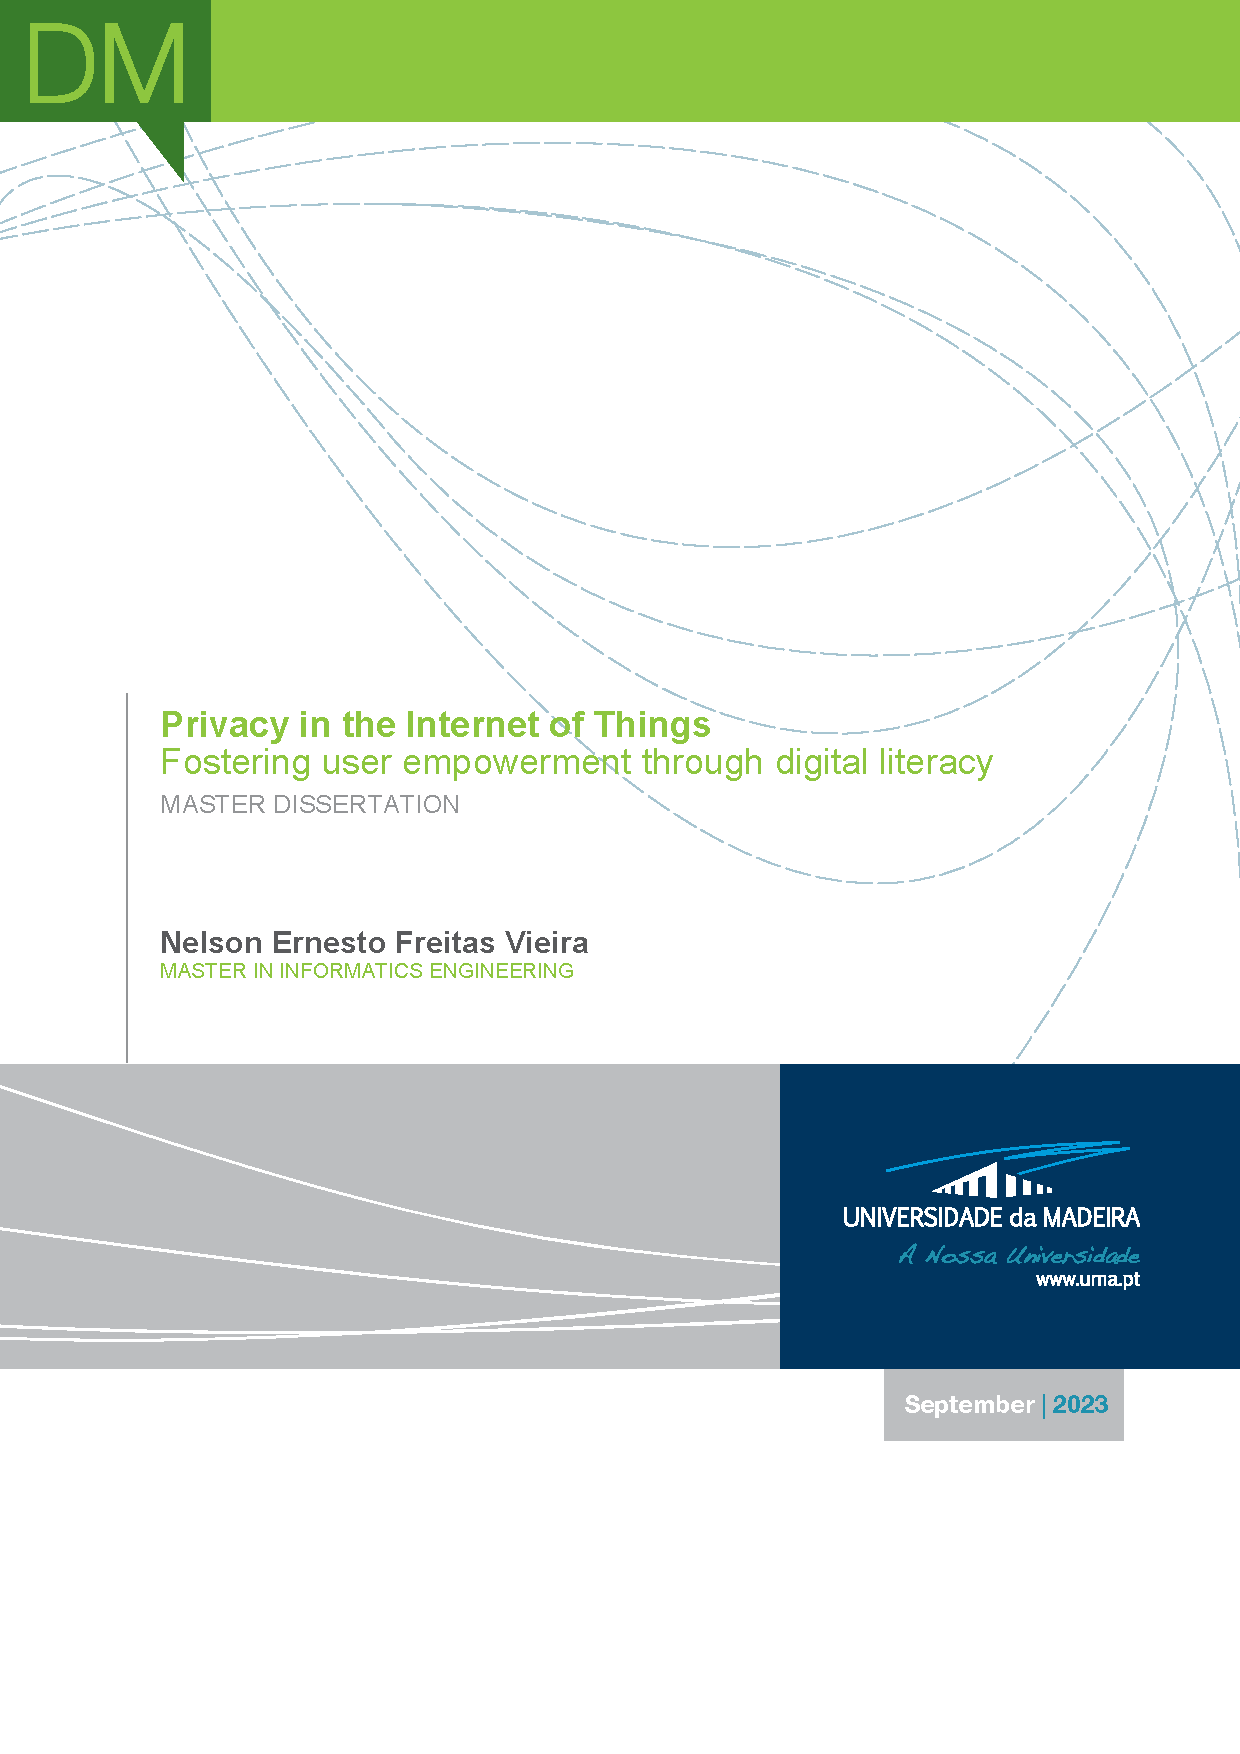
\includepdf[pages=-]{chapters/0_front_cover.pdf}
    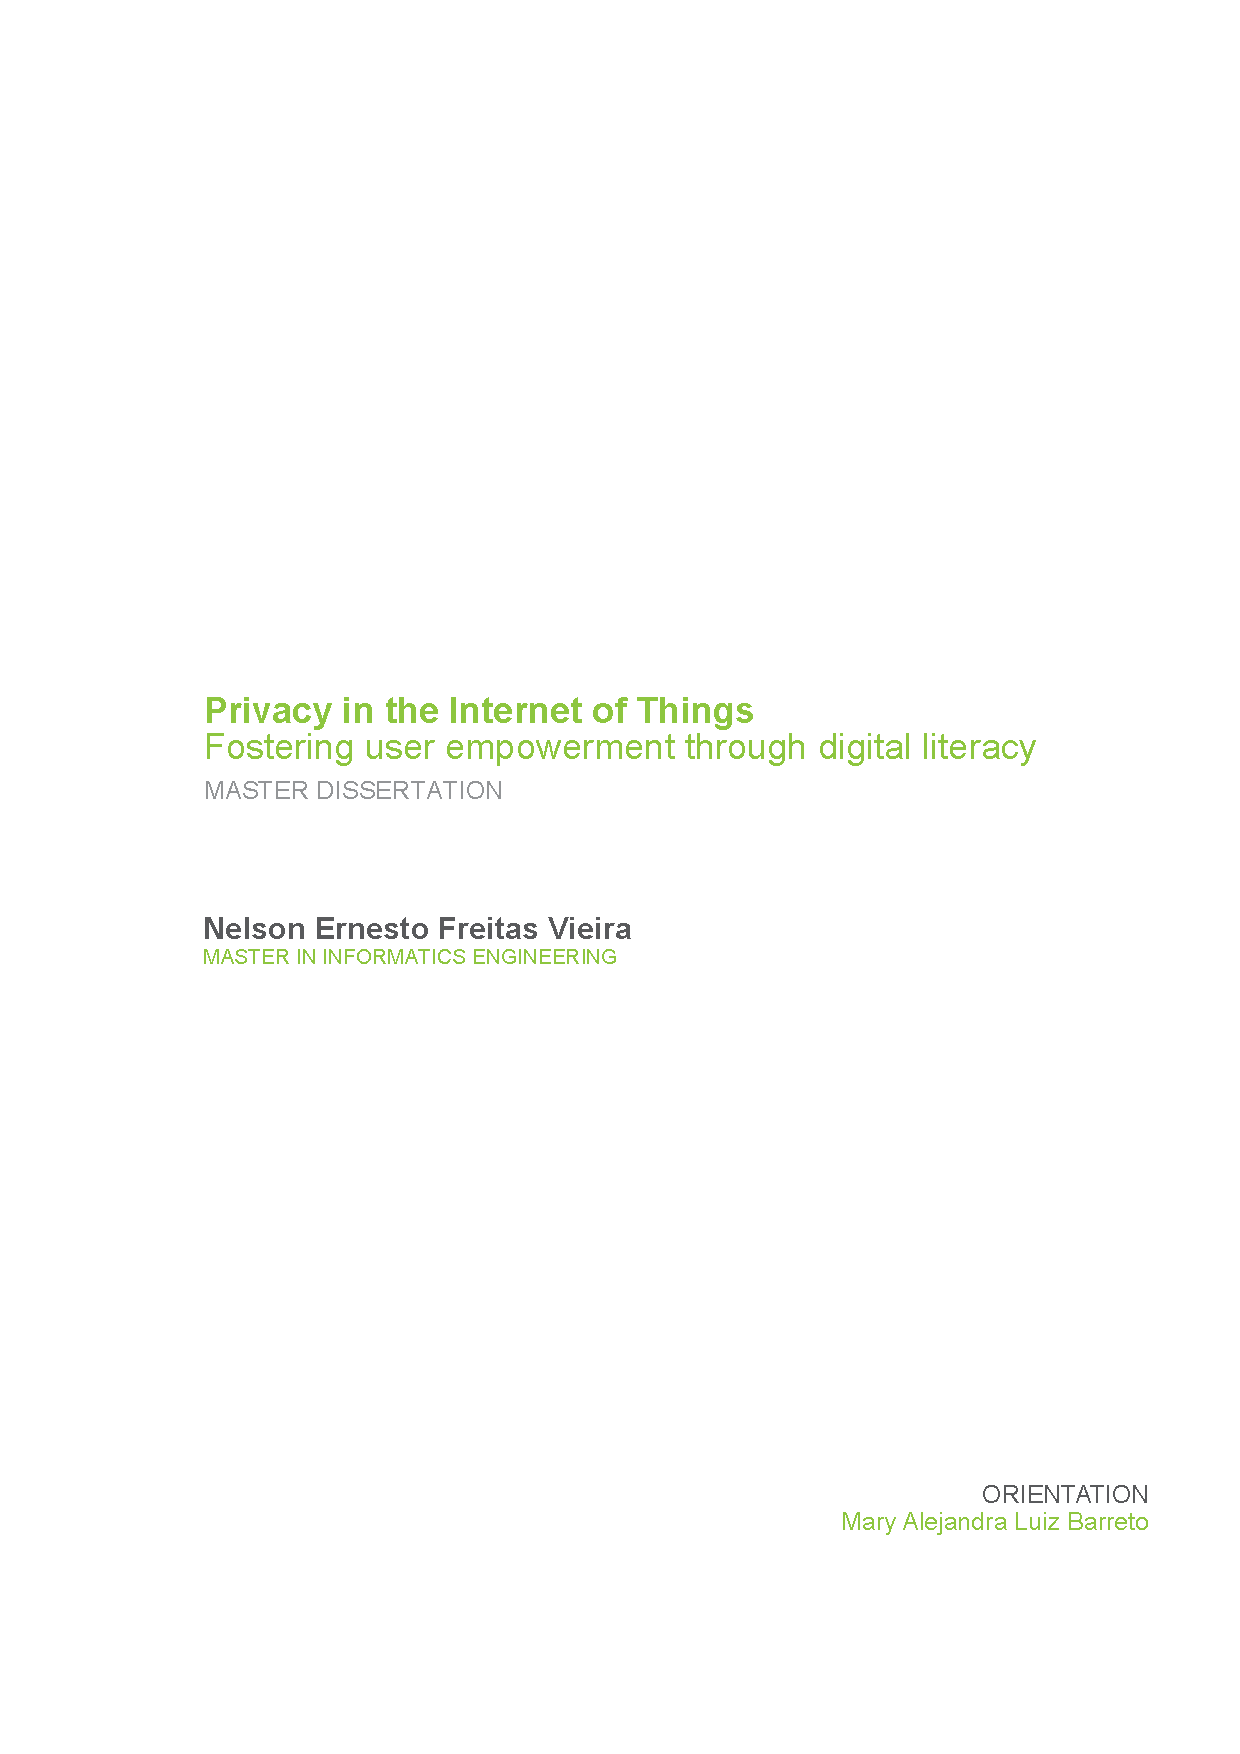
\includepdf[pages=-]{chapters/0_inner_cover.pdf}
    % SPDX-License-Identifier: CC-BY-4.0
%
% Copyright (c) 2023 Nelson Vieira
%
% @author Nelson Vieira <nelson0.vieira@gmail.com>
% @license CC-BY-4.0 <https://creativecommons.org/licenses/by/4.0/legalcode.txt>
\begin{titlepage}
    \centering
    \addtolength{\hoffset}{0.5cm}
    \centering
    
\includegraphics[width=0.50\textwidth]{assets/images/uma_logo.png}\par\vspace{0.5cm}
    {\scshape\LARGE \selectlanguage{portuguese} Faculdade de Ciências Exatas e da Engenharia \par}
    \vspace{1cm}
    {\scshape\Large Mestrado em Engenharia Informática \par}
    \vspace{1.5cm}
    {\huge\bfseries Privacy in the Internet of Things: Fostering User Empowerment through Digital Literacy \par}
    \vspace{2cm}
    {\Large Nelson Ernesto Freitas Vieira\par}
    \vfill
    {\large Orientado por: \par}
        Mary Alejandra Luiz Barreto\par
    \vfill
    {\large Constituição do júri de provas públicas: \par}
        Nome completo (categoria), Presidente \par
        Nome completo (categoria), Vogal \par
        Nome completo (categoria), Vogal \par
    \vfill
    % Bottom of the page
    {\large \bfseries \today \par}
\end{titlepage}

    % SPDX-License-Identifier: CC-BY-4.0
%
% Copyright (c) 2023 Nelson Vieira
%
% @author Nelson Vieira <2080511@student.uma.pt>
% @license CC-BY-4.0 <https://creativecommons.org/licenses/by/4.0/legalcode.txt>
\chapter*{Resumo}
\justify

Os dispositivos da Internet das Coisas estão por todo o lado, desde
o nascimento da computação ubíqua que se prevê que a vida quotidiana
do ser humano contenha milhões de dispositivos que controlam todos os
aspectos da nossa vida. Hoje em dia, temos veículos inteligentes, casas
inteligentes, cidades inteligentes, dispositivos vestíveis, entre
outros, que utilizam vários tipos de dispositivos e vários tipos de
redes para comunicar. Estes dispositivos criam novas formas de recolha
e tratamento de dados pessoais de utilizadores e não utilizadores.
A maioria dos utilizadores finais nem sequer tem conhecimento ou tem
pouco controlo sobre a informação que está a ser recolhida por
estes sistemas. Este trabalho adopta uma abordagem holística a este
problema, começando por realizar uma revisão da literatura para
compilar as soluções actuais, os desafios e as oportunidades de
investigação futura. Realizando, em seguida, um inquérito para saber mais
sobre o conhecimento geral dos indivíduos sobre privacidade, IoC e
hábitos \textit{online} e, finalmente, com base na informação recolhida,
é proposta uma aplicação móvel que fornece aos utilizadores informações
sobre os dispositivos que estão próximos e como proteger os dados
que não querem partilhar com esses dispositivos.
Os testes com utilizadores revelaram que os participantes valorizam
ter acesso a mais informações sobre termos relacionados com a privacidade.
Esta aplicação é capaz de detetar que tipo de dispositivos estão próximos,
que tipo de dados são recolhidos por esses dispositivos
e apresentar opções de privacidade ao utilizador, quando possível,
com o objetivo de fornecer aos indivíduos uma ferramenta para tomarem
decisões informadas sobre os seus dados privados.

\keywords{privacidade \and Internet das Coisas \and computação ubíqua \and desafios na IoC \and literacia digital}

    % SPDX-License-Identifier: CC-BY-4.0
%
% Copyright (c) 2023 Nelson Vieira
%
% @author Nelson Vieira <nelson0.vieira@gmail.com>
% @license CC-BY-4.0 <https://creativecommons.org/licenses/by/4.0/legalcode.txt>
\chapter*{Abstract}
\justify

Internet of Things devices are everywhere, since the birth of ubiquitous
computing, human everyday life is expected to contain millions of
devices that control every aspect of our lives. Today we have smart vehicles,
smart houses, smart cities, wearables among other things that use various
types of devices, and various types of networks to communicate. These devices
create new ways of collecting and processing personal data from users, and
non-users. Most end users are not even aware or have little control over
the information that is being collected by these systems. This work takes
a holistic approach to this problem by first conducting a literature review
to compile current solutions, challenges and future research opportunities.
Then conducting a survey to learn more about the general knowledge of
individuals about privacy, IoT and online habits, and finally, based on the
information gathered, a mobile application is proposed that gives users
information about nearby devices, and how
to protect the data that they do not want to share with them.
User testing revealed that participants valued having access to more
information about privacy related terms. This
application is capable of detecting what type of devices are nearby, what kind
of data is collected by these devices, and displaying privacy options to the user,
when it is possible to do so, with the goal of providing individuals a tool to make
informed decisions about their private data.

\keywords{privacy \and Internet of Things \and ubiquitous computing \and challenges in IoT \and digital literacy}

    % SPDX-License-Identifier: CC-BY-SA-4.0
%
% Copyright (c) 2023 Nelson Vieira
%
% @author Nelson Vieira <nelson0.vieira@gmail.com>
% @license CC-BY-SA-4.0 <https://creativecommons.org/licenses/by-sa/4.0/legalcode.txt>

\chapter*{Acknowledgment}

Agradeço ...




    \bfseries
    \tableofcontents
    \normalfont

    \listoffigures

    \listoftables

    % SPDX-License-Identifier: CC-BY-4.0
%
% Copyright (c) 2023 Nelson Vieira
%
% @author Nelson Vieira <nelson0.vieira@gmail.com>
% @license CC-BY-4.0 <https://creativecommons.org/licenses/by/4.0/legalcode.txt>
\chapter*{List of Acronyms}

% Source: https://latex.org/forum/viewtopic.php?t=16419

% Define a convenient command to add a line
% to the database
\newcommand*{\addacronym}[2]{%
    \DTLnewrow{acronyms}%
    \DTLnewdbentry{acronyms}{Acronym}{#1}%
    \DTLnewdbentry{acronyms}{Description}{#2}%
}

% Create the database
\DTLnewdb{acronyms}
\addacronym{IoT}{Internet of Things}
\addacronym{RFID}{Radio-frequency identification}
\addacronym{MIT}{Massachusetts Institute of Technology}
\addacronym{M2M}{Machine-to-machine}
\addacronym{IP}{Internet Protocol}
\addacronym{GDPR}{General data protection regulation}
\addacronym{CCPA}{California consumer privacy act}
\addacronym{SLR}{Systematic literature review}
\addacronym{PA}{Privacy assistant}
\addacronym{PPA}{Personalized privacy assistant}
\addacronym{SaaS}{Software as a service}
\addacronym{VPN}{Virtual private network}
\addacronym{IT}{Information technology}
\addacronym{VM}{Virtual Machine}
\addacronym{NIST}{National Institute of Standards and Technology}
\addacronym{ISO}{International Organization for Standardization}
\addacronym{RQ}{Research question}
\addacronym{DP}{Differential privacy}
\addacronym{BASE}{Bielefeld Academic Search Engine}
\addacronym{PbD}{Privacy-by-Design}

% Sort the database
\DTLsort{Acronym}{acronyms}

% Display the contents of the database
\begin{itemize}
\DTLforeach*{acronyms}{\thisAcronym=Acronym,\thisDesc=Description}%
    {\item[] \textbf{\thisAcronym} \thisDesc}%
\end{itemize}


    %% Fix for the nomenclature spacing
    \newlength{\nomitemorigsep}
    \setlength{\nomitemorigsep}{\nomitemsep}
    \setlength{\nomitemsep}{-\parsep}
    \newcommand\bparagraph[1]{\vspace{1.0mm}\noindent\textbf{#1.}}
    \hypertarget{abbr}{\printnomenclature{}}
    \clearpage

    \setcounter{page}{1}
    \pagenumbering{arabic}
    % \linenumbers
    % SPDX-License-Identifier: CC-BY-SA-4.0
%
% Copyright (c) 2023 Nelson Vieira
%
% @author Nelson Vieira <nelson0.vieira@gmail.com>
% @license CC-BY-SA-4.0 <https://creativecommons.org/licenses/by-sa/4.0/legalcode.txt>

%%% CHAPTER 1/Capitulo 1
%
\section{Introduction}

Privacy as we know it is a somewhat recent concept \cite{vincent2016privacy, moore2017privacy},
before the digital age there was barely any notion of privacy for most
people. For many centuries most people used to reside in small communities
where they were continuously involved in one another's lives. Even more
recent is the idea that privacy is a crucial component of personal security,
in contrast to the undeniable necessity of public security, including the
requirement for guarded walls and closed doors. Long seen as a luxury, privacy
is still usually regarded as a good to have rather than an essential
requirement, even though it is acknowledged as a human right, as present
in article 12 of the Universal Declaration of Human Rights \cite{RooseveltUniversal}:
``No one shall be subjected to arbitrary interference with his privacy,
family, home or correspondence, nor to attacks upon his honour and reputation.
Everyone has the right to the protection of the law against such interference
or attacks''. Privacy can be defined \cite{InternationalWhat, SpiekermannEngineering}
as the right to govern how personal information and data is collected, stored,
and used, it frequently involves handling sensitive information with care,
and as such, organizations must be open and honest about the kind of data
they plan to gather, why they need it, and where and with whom they plan
to share it. Users should have the right to control their shared information.

This definition can cause some confusion with the idea of security \cite{HIVDifference}
and although privacy and security are interconnected, security involves
measures taken to safeguard data from risk, threat or danger, it frequently
alludes to safety. It is the practice of keeping users' personal information
and data safe and preventing unauthorized access to it. The primary contrast
between privacy and security is that the former deals with personal information
to individuals and how they want their data used and maintained, whilst
the latter deals with its protection from possible threats. Security can
exist without privacy, but the opposite is not true. For managing sensitive
and personal data, privacy and computer security are equally crucial. Users
should be aware of the internal procedures regarding the collection, processing,
retention, and sharing of personal information.

Concerns about digital privacy have been growing \cite{emami2019exploring, park2022personal, zhang2022peer}
in the last few years, especially after the Anonymous decentralized hacker
group cyber attacks, WikiLeaks and Snowden's leaked top secret documents
from United State's National Security Agency. These concerns can be noted
with the increase of written literature on the subject, when searching for
terms like ``privacy'', ``online privacy'', ``digital privacy'' in Google
Scholar, ACM Digital Library or Science Direct it can be seen that, in the
last 5 years, it returns about 5000000, 650000 and 80000 documents respectively,
including articles, books, conference papers etc.

Most research has focused on the web, while privacy in IoT systems has not
been explored as much. Because IoT devices are becoming more prevalent,
new methods of communicating, gathering, and analyzing data emerge.
Because there is already a substantial quantity of research focusing on
web privacy rather than IoT privacy, it is a lot more fertile ground to
explore the issue of privacy in the context of the IoT.

\textit{Internet of Things} is a term that first appeared in the 1990s,
and it may be linked to Mark Weiser's paper on ubiquitous computing \cite{weiser1991computer}
and the growth of devices of all sizes that communicate with one another
to do various tasks, making Weiser's dream a reality. The first use of the
term \textit{Internet of Things} was in 1999 by British technology pioneer
Kevin Ashton \cite{KevinThat}, executive director of the Auto-ID Center
at Massachusetts Institute of Technology (MIT), to describe a system in
which items may be connected to the internet by sensors. He came up with
the phrase while giving a presentation for Procter \& Gamble to highlight
the value of linking Radio-Frequency Identification (RFID) tags used in
corporate supply chains to the internet in order to count and track goods
without the need for human assistance. These devices are used in various
applications, starting at home \cite{marikyan2019systematic} with thermostats,
fridges, microwaves, etc, moving on to smart cars \cite{arena2020overview},
the educational system \cite{al2020survey}, our clothes and our watches \cite{niknejad2020comprehensive}
and even into outer space \cite{AkyildizInternet}. IoT resources may include
IoT equipment (like smart home assistants and autonomous vehicles), IoT
services (like video analytics services linked to smart cameras and indoor
position tracking systems), or IoT apps (like smart TV remote apps) that
track and use information about us. Internet of Things is now widely used
to describe situations in which a range of objects, gadgets, sensors, and
ordinary items are connected to the internet and have computational capabilities.

The idea of using computers and networks in order to monitor and manage
devices is nothing new, despite the term \textit{Internet of Things} being
relatively recent.
% By the late 1970s, technologies for remotely monitoring electricity
% grid meters through telephone lines were already in use in the corporate
% sector \cite{}.
Wireless technology improvements in the 1990s permitted the widespread
adoption of corporate and industrial machine-to-machine (M2M) solutions
for equipment monitoring and operation. Many early M2M solutions, on the
other hand, relied on proprietary purpose-built networks or industry-specific
standards rather than internet standards. To connect devices other than
computers to the internet is not a new concept. A Coke machine at Carnegie
Mellon University's Computer Science Department \cite{EverhartInteresting}
was the first ubiquitous device to be linked to the internet. The system,
which was created in 1982, remotely observed the out of stock lights on
the pressing buttons of the vending machine and broadcast the state of each
row of the vending machine on the network so that it could be accessed using
the Name/Finger protocol through a terminal. In 1990, a toaster that could
be turned on and off over the internet that was created by John Romkey \cite{RomkeyToast},
was demonstrated at the Interop Internet Networking show.

% \cite{rose2015internet}
% The term "Internet of Things" (IoT) was first used in 1999 by British technology
% pioneer Kevin Ashton to describe a system in which objects in the physical world
% could be connected to the Internet by sensors.12 Ashton coined the term to
% illustrate the power of connecting Radio-Frequency Identification (RFID) tags13
% used in corporate supply chains to the Internet in order to count and track goods
% without the need for human intervention. Today, the Internet of Things has become
% a popular term for describing scenarios in which Internet connectivity and computing
% capability extend to a variety of objects, devices, sensors, and everyday items.

% While the term "Internet of Things" is relatively new, the concept of combining
% computers and networks to monitor and control devices has been around for decades.
% By the late 1970s, for example, systems for remotely monitoring meters on the
% electrical grid via telephone lines were already in commercial use. In the
% 1990s, advances in wireless technology allowed "machine-to-machine" (M2M)
% enterprise and industrial solutions for equipment monitoring and operation to
% become widespread. Many of these early M2M solutions, however, were based on closed
% purpose-built networks and proprietary or industry-specific standards, rather than
% on Internet Protocol (IP)-based networks and Internet standards. Using IP to connect
% devices other than computers to the Internet is not a new idea. The first Internet
% "device"—an IP-enabled toaster that could be turned on and off over the Internet—was
% featured at an Internet conference in 1990. Over the next several years, other
% "things" were IP-enabled, including a soda machine at Carnegie Mellon University in
% the US and a coffee pot in the Trojan Room at the University of Cambridge in the UK
% (which remained Internet-connected until 2001). From these whimsical beginnings, a
% robust field of research and development into "smart object networking" helped
% create the foundation for today's Internet of Things.

The Internet of Things can be defined as: ``An open and comprehensive network
of intelligent objects that have the capacity to auto-organize, share information,
data and resources, reacting and acting in face of situations and changes
in the environment'' \cite{madakam2015internet}.

IoT is one of the fastest growing technologies \cite{MohammadState}, it
is predicted that it will grow into the trillions of devices by 2030 \cite{SarawiInternet},
and with this expansion new security vulnerabilities and data gathering
dangers appear, the lack of security in these devices makes them ideal targets
for privacy violations and inadequate customer disclosure of device capabilities
and data practices aggravates privacy and security issues.

Privacy in IoT systems in not seen as a crucial factor in development \cite{alhirabi2021security}.
Specific standards for privacy options have been imposed by data privacy
regulations including the General Data Protection Regulation (GDPR) and
California Consumer Privacy Act (CCPA), but even these regulations have
been criticized \cite{peloquin2020disruptive, gladis2022weaponizing, gentile2022deficient, green2022flaws, byun2019privacy}.

\subsection{Título subsecção}

ABC

\subsection{Título subsecção}

ABC

\subsection{Estrutura do Documento}

    \clearpage
    % SPDX-License-Identifier: CC-BY-4.0
%
% Copyright (c) 2023 Nelson Vieira
%
% @author Nelson Vieira <nelson0.vieira@gmail.com>
% @license CC-BY-4.0 <https://creativecommons.org/licenses/by/4.0/legalcode.txt>
\section{State of the Art}

\par
This section provides an overview of the recent literature with the themes
that were found to be more relevant for this work.

\subsection{Privacy Paradox}

The use of a variety of digital devices have numerous advantages, but they
also bring with them the ubiquity of data capturing equipment, therefore,
it is understandable why the majority of online users have serious concerns
about the privacy of their personal data. However, the opinions expressed
are starkly at odds with the reality, according to Thomson et al. \cite{DarrenState}
report on the state of privacy, that just one in four European users read
the terms and conditions in their entirety prior to making an online purchase
or subscribing to a service, 59\% admitted to only quickly scanning the
terms and conditions before completing a purchase, while 14\% admitted to
never reading them at all, 30\% of the respondents would even swap their
email address to win a reward, or entry into a raffle, while 17\% would do
so to get an app and 30\% would do it for money.

This is what is called a privacy paradox, there have been multiple papers
written on this subject \cite{solove2021myth, WilliamsPrivacy, lee2021investigating, goad2021privacy, gerber2018explaining},
some papers attempt a theoretical explanation while others attempt an empirical
one. There has been very different interpretations or explanations of this
paradox, a few papers \cite{wilson2012unpacking, warshaw2015can, lee2015privacy}
apply the theoretical concept of the \textit{homo economicus} \cite{zak2008moral},
which is the representation of people as beings who constantly act in a
way that is logical and self-interested, not worrying about morality or
ethics, and who do so to the best of their ability, to the context of privacy.
Individuals' decision-making processes can be greatly influenced by a variety
of cognitive biases and heuristics, and these decisions can vary greatly from
individual to individual, according to several studies on individual choice behaviour \cite{acquisti2007can, knijnenburg2013dimensionality, wakefield2013influence, flender2012type}.
According to several articles \cite{dienlin2015privacy, baek2014solving},
this paradox might be explained by the fact that some people have genuinely
experienced online privacy assaults and that most privacy views are therefore
based on heuristics or second-hand accounts. Taddicken's study \cite{taddicken2014privacy}
argues that peer pressure is the reason people have this contradictory behaviour,
Norberg et al. \cite{norberg2007privacy} explains this paradox by suggesting
that while perceived risk affects reported attitudes and behavioural intentions,
trust has a direct impact on privacy behaviour, while others \cite{flender2012type, kokolakis2017privacy}
rely on quantum theory, meaning there is indeterminacy in the decision making,
in other words, it means that an individual's decision's result can be determined
at the time of the decision and not before. Brandimarte et al. \cite{brandimarte2013misplaced}
have explored the idea that when it comes to their data privacy, users have
an \textit{illusion of control}.

This paradox has been proven to be vitiated by a number of empirical studies \cite{dienlin2015privacy, xie2019consumers, SCHWAIG20131, sannon2018privacy},
online privacy practices are founded on separate privacy mindsets and so
they are not inherently paradoxical.

\subsection{Privacy in IoT: Approaches}

There have been a number of systematic literature reviews (SLRs) \cite{Gupta2022Privacy, Kuhtreiber2022survey, sicari2015security, LinSurvey, yang2022overview, zubaydi2023leveraging}
and systematic mapping reviews \cite{porras2018security, ahmed2019aspects}
done to study privacy and security issues in IoT.

In Gupta and Ghanavati's \cite{Gupta2022Privacy} SLR, the authors review
papers with methodologies and techniques that identify privacy risks or
notify users about these risks. They divide the literature into the following
categories: `Ontological Modeling and Semantic-based Approaches', `Data-Driven
Approaches', `Source Code Analysis-based Approaches', `User Studies and
Survey-based Approaches', `Blockchain-based Approaches' and `Architectural
and Framework-based Approaches'. They then examine current literature on
these three prerequisites. The findings show that: most works concentrate
on single IoT devices when addressing privacy threats; When analysing privacy
issues, key privacy factors such as data reduction and data aggregation
are overlooked; existing studies ignored the sensitivity of the obtained
information; most useful studies did not include a diverse range of users
when assessing privacy problems; no work has been done to discover compliance
difficulties between an IoT application and different privacy rules; and
current research does not place a premium on providing individuals with real-time
privacy notices. However, this SLR has the following limitations: the authors
only chose articles and not thesis or books and from the selected papers,
only the ones written in english were considered.

Kühtreiber et al. \cite{Kuhtreiber2022survey} evaluate the frameworks and
tools established for developers, specifically in the case of IoT, and find
that current solutions are difficult to use, only successful in limited
scenarios, and insufficient to handle the privacy problems inherent in IoT
development. This study lacks a comprehensive gap review of the chosen
literature, along with research questions (RQs) establishing the significance
of the articles chosen.

Sicari et al. \cite{sicari2015security} examine current research and ongoing
activities that focus on IoT privacy and security solutions. The authors
start by describing the requirements for IoT privacy and security, such
as access control, confidentiality, and authentication. The authors then
conduct a literature study in connection to these three needs. The authors
came to the conclusion that IoT privacy issues have only been partially
examined and that further attention is required. The study does, however, have
some shortcomings: the prior research analysis focuses primarily on security
requirements while ignoring privacy considerations; the authors do not conduct
a thorough gap analysis on the publications examined; and they do not provide
a comprehensive summary of future research topics in the area of IoT privacy
that require more attention.

Lin et al. \cite{LinSurvey} undertake a literature review to identify security
and privacy vulnerabilities in the three IoT architecture layers: network,
perception, and application. The authors describe the first six fundamental
security properties for these tiers as confidentiality, integrity, availability,
identification and authentication, privacy, and trust. Then, the authors
look at a variety of security threats for each of the three stages. The
authors wrap up by giving a succinct summary of many privacy-preserving
data techniques, including the stages of data collection, data aggregation,
and data analysis. The authors do, however, largely focus on the IoT's security
components and consider privacy to be one of the most crucial security aspects,
rather than viewing privacy as a distinct concern. Despite this, the authors
devote a portion of the paper to privacy and the majority of what they address
concerns security.

Yang's study \cite{yang2022overview} examines the literature from the perspective
of IoT phases, such as data collection, transmission, and storage, or in other
words, perception, network and application layers. In these phases the author explores
security protocols at the physical layer, network solutions, and data storage and
sharing approaches. There is a balance of security approaches or solutions and
non-security related approaches discussed, besides the mentioned security protocols,
the author proposes a software-defined network, for the network layer, that enables
a global view of the network which helps to identify malicious traffic patterns. The
author also suggest the use of differential privacy, privacy-preserving data mining,
blockchain or holochain for the application layer. The author presents a high-level
overview of privacy issues and as a result does not offer a comprehensive analysis of
the various approaches or make many suggestions for future study directions.

In Zubaydi et al. \cite{zubaydi2023leveraging}, different works that address the
integration of blockchain technology that aim to tackle various aspects of privacy
are analysed. This SLR has an overview of the IoT architecture, the various blockchain
types and algorithms and IoT challenges. The authors provide an overview of the
chosen papers and present a detailed comparison between them before analysing
the papers using several categories which include generic approaches, healthcare,
smart environments, IoT device gateway, IoT information systems, management systems
and other approaches. The authors also present a considerable number of open issues
that future works should focus on. Because this SLR is about blockchain technology,
the focus is on privacy through security. Overall this is a very in-depth SLR on the
use of blockchain technology to address privacy issues.

Khanna and Kaur \cite{khanna2020internet} make a literature overview...
% ! to expand

Based on Ziegeldorf's \cite{ziegeldorf2014privacy} analysis of the literature,
the following are the most prominent privacy concerns in IoT:

\begin{enumerate}
    \item
    The most prominent concern is \textit{identification}, which binds an
    identifier, such as a name and location, with an individual's identity,
    this also enables and aggravates other threats;
    \item
    \textit{Localization and tracking} is the threat of detecting an individual's
    locations through numerous techniques, such as GPS, internet traffic,
    or smartphone location. This threat requires \textit{identification}
    of some kind;
    \item
    In e-commerce, \textit{profiling} is often used for personalization.
    Organizations collect information about individuals in order to deduce
    their interests via association with other profiles and data sources.
    \item
    \textit{Interaction and presentation} allude to the sharing of private
    information with an unintended audience while doing so through a public
    medium. IoT applications often need extensive user interaction, it is
    expected that users of these systems will obtain information via smart
    devices in their immediate surroundings and that users will interface
    with systems in creative, natural ways. However, many of those modes
    of communication and presentation are already available to the broader
    public, making them apparent to anybody around. When personal information
    is transferred between a system and its user, privacy is breached.
    \item
    \textit{Lifecycle transitions} occur when an IoT device is sold, utilized
    by its owner and eventually disposed of. There may be an expectation
    that the object deletes all information, yet smart devices frequently
    keep massive volumes of data about their own past throughout their entire
    existence. This might contain personal images and videos, which are
    not always erased following ownership transfer.
    \item
    \textit{Inventory attacks} involve unauthorized entry and the acquisition
    of information about the presence and characteristics of personal things.
    Malicious users might use inventory data to profile the property and
    break in.
    \item
    \textit{Linkage} is the process of connecting disparate systems, when
    systems are connecting different data sources, there is a higher danger
    of unauthorized access and data leakage.
\end{enumerate}

Another concept worth analysing is differential privacy (DP) which relates more
closely to the survey that will be conducted but also to the general
collection and analysis of user data by applications and systems.

\subsection{Differential Privacy}

The notion of differential privacy, according to Michael Kearns \cite{kearns2019ethical},
is based on three important principles. The first being that ``differential
privacy requires that adding or removing the data record of a single individual
not change the probability of any outcome by much''. The second principle
being that ``no outside observer can learn very much about any individual
because of that person's specific data''. And the third important principle
being that ``for every individual in the dataset, and for any observer no
matter what their initial beliefs about the world were, after observing
the output of a differentially private computation, their posterior belief
about anything is close to what it would have been had they observed the
output of the same computation run without the individual's data''.

DP has the potential to significantly increase individual
privacy protection, by purposefully adding noise into a dataset, it gives
plausible deniability to any individual who may have had their data exploited
while still being able to calculate statistics with relatively high precision.
Although algorithms that deal with notions of fairness, ethics, and privacy
are hard to implement because of the subjectivity of these concepts, and
DP algorithms are no exception, they can still help in
regards to tackling technology's intrinsic ethical and moral issues.

Zhao and Chen \cite{ZhaoSurvey} conduct a SLR on DP for
unstructured data. The authors present DP methods for
sensitive content in image, audio, video, and text data. They compare the
various methods and perform utility analyses for each method, highlighting
the benefits and drawbacks of each, the utility loss is measured in experimental
evaluations between the actual data and its obfuscated variant. They come
to the conclusion that DP as well as its variations give
stringent privacy protections for unstructured data against attackers with
unpredictable background knowledge. They also suggest potential future study
subjects that have yet to be investigated.

Integrating federated learning and local differential privacy is proposed
by Zhao et al. \cite{zhao2020local} to facilitate crowdsourcing applications to
achieve the machine learning model while avoiding privacy threats and reducing
communication costs. The authors provide four mechanisms depending on the
privacy budget that is wanted. Based on experimental results of real-world
datasets, the suggested mechanisms provide stronger privacy protection when
compared to other comparable mechanisms; nevertheless, further testing is
required to establish the validity of these mechanisms on production systems.
No future research subjects are provided, only the intention of applying
these mechanisms to deep neural networks.

Similar to differential privacy, there exists different algorithms that aim to
preserve privacy such as Google's box blurring algorithm \cite{FromeLarge}
that is used in the Google Map's street view, Microsoft's Visor \cite{poddar2020visor}
which is a video-analytics-as-a-service tool and Shokri and Shmatikov's
\cite{ShokriPrivacy} system for collaborative deep learning, however, in
general, these algorithms struggle with high computational cost, internal
attacks, or non-provable privacy.

\subsection{Proposed Solutions}

\par This section presents a variety of solutions separated by themes that arose
from the structured literature research in order to address the disconnect
between privacy ideas across systems and users.

\subsubsection{User Awareness}

Although individuals have a certain expectation of privacy when using IoT
devices, privacy preferences are complex, as noted by \cite{naeini2017privacy},
some individuals value some aspects more than others. There are multiple studies
on privacy in IoT but not many focus on user privacy awareness or
privacy literacy.

Koohang et al. \cite{koohang2022internet} propose a research model with
the goal to examine the relationship between IoT awareness and IoT privacy,
security, and trust, and how this influences IoT continuing usage. To validate
the model, they conducted a study with 299 participants and discovered that
as users increase their awareness of IoT security and privacy threats, their
privacy and privacy knowledge increases, and as users become savvier about
IoT privacy and security, they place more trust in IoT devices, which affects
their continued intention to use these IoT devices. Previous publications
provide support for the proposed model like \cite{tsourela2020internet, knijnenburg2022modern}.
The authors acknowledged the method's shortcomings due to use of a traditional
statement-based method survey in the study and proposed a scenario-based
method approach and a random sample to validate the results, but they did
not elaborate any further on future research directions.

An interactive theatre experience was developed by Skirpan et al. \cite{SkirpanPrivacy}
as a case study of an innovative approach to gather user awareness about their
online behaviour with regard to privacy. This was created to try to prove
that a simulated experience with a credible privacy problem may encourage
people to take action before actually encountering a catastrophe. The plot
of the play consist in a fledgling tech company that unveiled its revolutionary
artificial intelligence (AI) technology while dealing with a company whistleblower and an untimely
zero-day hack on their system. The public is able to interact with the actors
and influence how the story plays out. Audiences and actors were given the
chance to try on roles, behaviors, and opinions that they would not normally
have access to in ordinary life. The authors had interviews and surveys
done after the plays with audience members however they only did interviews
halfway through production and only a small fraction of the audience actually
participated in this data collection, they also noted that after contacting
people months after the interviews that they did not really changed their
behaviour regarding their privacy rights.

\subsubsection{Legislation}

Some papers seek to improve legislation \cite{WEBER2015618, FabianoInternet}
because otherwise, in their view, privacy rights won't be respected if they
are not enforceable legally, they defend that without the express agreement
of the individual concerned, private information obtained by IoT devices
must not be retained or processed in any form, and necessary procedures
must be taken to guarantee that the data collected is not that of an unrelated
individual. But better protection laws for the user would also create opposition
from most companies that want to extract as much private data from their
users without (m)any restrictions in order to increase their profit margins.

The research conducted by Hadzovic et al. \cite{hadzovic2023path} focuses on
present initiatives aimed at establishing an IoT and AI regulatory and legislative
framework in the European Union (EU), as well as its pertinence in developing nations, the authors
choice to focus on EU is due to EU's claim for becoming a global leader \cite{european2021europe}. The authors
identify three steps toward the development of an IoT and AI regulatory and
legislative framework. The first step is to develop a national AI strategy, which
is an important blueprint for increasing AI adoption and should be developed
in accordance with a country's strategic priorities. To that end, a proactive
information and communications technology (ICT) regulator could initiate and encourage
national AI strategy development. The second step in developing a regulatory
framework for IoT and AI involves the consideration of various aspects of IoT
and AI and navigating through many overlapping policy areas to determine the rules.
The legislation must be designed to be future-proof and not restrict technological
development. The ICT regulator, which plays a central role in improving innovation
and developing the electronic communications market, could also play a central role
in the context of IoT and AI. It could serve as a coordinating authority within
an advisory committee before the establishment of a national supervisory authority
for AI. The new regulatory framework should be prepared and assessed using the regulatory
impact assessment (RIA) method to select the best option for the country. And the
third step in the development of a regulatory framework for IoT and AI involves
redefining the role of regulatory authorities. The state must establish a national
supervisory authority, but it is also important to involve civil society, the private
sector, and academia in the process to ensure success. This approach is known as
multistakeholder governance development.

\subsubsection{Privacy through Security}

Sun et al. \cite{SunSecure} design a lightweight communication strategy
for a remote-control system, employing two types of Virtual-Spaces to achieve
the aim of identity announcement and data exchange. They constructed a prototype
system of the scheme and tested it on the Freenet, demonstrating that the
method can effectively resist the influence of flow analysis on communication
anonymity while preserving communication data security.

% ! to expand

\subsubsection{Architecture / Frameworks}

Antunes et al. \cite{AntunesFederated} do a SLR on federated learning in
the area of healthcare and make an architecture proposal. The procedure
known as federated learning allows for the distributed training of machine
learning models using remotely hosted datasets without the requirement to
gather and hence jeopardize data. The fundamental goal of the proposed architecture is
to allow healthcare institutions that have access to sensitive medical information
to use it in distributed data analysis and machine learning research while
ensuring patient confidentiality. Because information transmitted among
institutions need confidentiality guarantees for learning model parameters
and analysis results, the architecture can adopt a number of ways based on
a zero-trust security paradigm \cite{ChenSecurity}. Furthermore, the institutions
develop a learning algorithm verification system that can store and disseminate
manifestos, as well as engage in distributed analytic procedures that need
unanimous agreement from all participants. This study also demonstrates
that previous literature implies that homomorphic encryption and differential
privacy are effective approaches for preventing data breaches without incurring
prohibitively high computing costs.

Opara et al. \cite{opara2022framework} present a system for spotting possible
problems with privacy or security regulations in the early stages of development,
this approach is intended at developers. The paper proposes a domain-specific
ontology for modelling IoT security and privacy policies, a notation for
representing and validating IoT security and privacy policies, a set of
guidelines and rules for detecting IoT policy errors, and a tool for visually
modelling and capturing IoT security policies and discovering policy problems.
Although the framework that is presented is theoretically promising it has
not been tested in a real environment so the effectiveness can't yet be
measured. The authors also do not compare their proposal with others already
available.

A Privacy by Design (PbD) framework is proposed by Perera et al. \cite{perera2020designing}
to assist software developers in incorporating concerns about data privacy
into the design of IoT applications. The proposed framework consists in
a set of guidelines. The authors conducted two studies, one interview based
in person and the other online, the first study was done with software engineers with
various levels of experience and the second was done with master's students.
The authors note that developers do not have a privacy mindset, meaning
they do not regard privacy as an primary aspect of the application design,
giving more importance to other aspects like functionality or security.
They also mentioned that using this framework must be context-based, since
it may be difficult and prone to over-analysis by engineers. When citing
related works, they state that various PbD frameworks exist but none are dedicated
to IoT, which is incorrect as evidenced by other works \cite{o2017privacy, cavoukian2016embedding},
with \cite{alkhariji2023semantics, aljeraisy2021privacy} being more recent
examples. It is true, however, that there are relatively few IoT PbD frameworks.

\cite{zhang2017privacy} proposes a model for...
% ! to expand

There exists frameworks like the NIST Cybersecurity Framework \cite{barrett2018framework},
published by the National Institute of Standards and Technology (NIST),
which includes a number of recommendations for reducing organizational
cybersecurity risks. Although this framework is primarily focused on
security, it can also be used to reduce privacy threats.
ISO/IEC 27400:2022 \cite{iso2022cybersecurity}, developed by the International
Organization for Standardization (ISO), is a standard that provides
guidelines on risks, principles and safeguards for the security and
privacy of IoT systems. In addition, ISO has produced about 208 privacy-related
standards \cite{iso2023privacysearch}, some of which have been published
and others of which are currently in development. This is a small number
when compared to the roughly 1305 security-related standards \cite{iso2023securitysearch},
but there may be some overlap between these standards. Even those ISO privacy
based standards have a good amount of intersection with security related
guidelines.

\subsubsection{Blockchain}

Blockchain is an option to guarantee privacy in IoT because of zero-knowledge
proofs\cite{sun2021survey}, ring signatures \cite{mercer2016privacy} and mixing \cite{stone2021trustless}
among other techniques \cite{zhang2019security}.

A zero-knowledge proof is a cryptographic technique that enables one party
to demonstrate to another that a certain statement is true without disclosing
any information other than the validity of that statement. Completeness, soundness,
and zero-knowledge are the three requirements that must be satisfied by a
zero-knowledge proof method. Completeness states that if a
statement is genuine, an honest party will be convinced of it by another honest
party. Soundness indicates that a nefarious party should only have a small chance
of convincing an honest party that a statement is true. Zero-knowledge states
that the method must only tell one party whether or not the other party is
disclosing the truth.

Ring signatures create a single, recognizable signature that is used to sign
a transaction by combining a number of partial digital signatures from diverse
users. This group, known as the ring, can be chosen at random from the outputs
that other users have made to the blockchain. A ring signature has the security
property that it should be computationally expensive to determine which
of the group's members' keys was used to produce the signature, this is because
it obfuscates the input side of a transaction. A user's anonymity cannot
be taken away from their signature, and any group of users can act as a signing
group automatically.

Mixing is the process of blending possibly traceable digital assets
with others to obscure the original assets' sources. This is frequently done
by pooling source assets from different inputs for a long period and at random
intervals, then spitting them back out to destination addresses. Since they
are all packed together and then delivered at random intervals, it is very
difficult to pinpoint particular assets. Due to the fact that cryptocurrencies
provide a public record of every transaction, mixers have been developed
to improve cryptocurrency privacy. Because of their emphasis on secrecy,
mixers have been used to launder money using cryptocurrency.

Zhang et al. \cite{zhang2019security} outline some disadvantages concerning
these techniques. For example, the authors assert that zero-knowledge proofs
are less efficient than other techniques, that ring signatures cannot reveal
the identity of the signer in the event of a dispute, and that centralized
services run an increased risk of leaking users' personal information when
it comes to mixing.

Yu et al. \cite{yu2018blockchain} discuss various implementations of blockchain
that provide privacy through security, based on different categories like
data integrity, data sharing and authentication and access control, most
implementations proposed use a peer-to-peer network based on the Ethereum
platform, with the exception being using any consortium or private blockchain,
consortium meaning a blockchain where consensus is managed by a pre-selected set
of nodes and private meaning access permission and read/write authority are
tightly controlled. The authors use privacy as a proxy for security, they also
do not discuss the weak and strong points of each implementation or make any
comparison, they also do not provide further research questions.

Ali et al. \cite{AliIoT} suggest a software stack that combines peer-to-peer
file sharing with blockchain smart contracts to offer IoT users control
over their data and do away with the necessity for centralized IoT data
management. Blockchain smart contracts are used in the proposed `modular
consortium' architecture to regulate access while establishing responsibility
for both data owners and other parties that users grant access to.

\subsubsection{Privacy Assistants}

There exists a number of privacy assistants in the market. Privacy assistants
have the objective of giving the user flexibility in choosing the preferred
privacy options in available applications, most are used in smartphones,
very few are made for devices in the IoT.

The Carnegie Mellon University CyLab, which is the university's security
and privacy research institute, started developing in 2019 an IoT Infrastructure
that intended to be free of privacy leaks and software covered by their
Secure and Private IoT Initiative 2019, this project would fall under
their main research theme of Trust. In this project they started the design
of a Personalized Privacy Assistant (PPA) \cite{ColnagoInforming}, this
would involve the use of semi-structured interviews with 17 participants
to examine user perceptions of three hypothetical PPA implementations,
each of which is potentially more autonomous, while outlining the advantages
and disadvantages of each implementation. The interviews were divided into
three sections: exploratory, anchoring and the PPA; While the exploratory
phase's purpose was to learn about participants' attitudes and understanding
of IoT, the anchoring phase aimed to normalize participants' basic understanding
of how IoT functions. In order to get people to think about potential privacy
concerns towards the end of the anchoring section, the authors asked participants
about their opinions on data privacy. In the PPA section, it was proposed
the idea of a PPA for IoT as a potential future project. The authors clarified
that the PPA could distinguish between active data requests such as a gadget
asking biometric information from the user's health tracker and passive
data collection such as a smart device with a microphone that could record
people's utterances while they were nearby. The Notification, Recommendation,
and Auto implementations of an IoT PPA were the three that the authors and
attendees discussed. Notification PPAs can determine which adjacent devices
are requesting data and alert users to those devices' presence and requests
so that users can approve or reject each request. Building on notification
PPAs, recommendation PPAs offer advice to individuals on how to share their data
based on their preferences. The user's data sharing decisions would be made
by auto PPAs. This would lessen the cognitive load on individuals but also
take away their ability to influence the process. They found that the participants'
attitudes regarding the various implementations were generally favourable,
although they also voiced worries, which varied depending on the degree
of automation. Given the divergent motivations of participants some desired
increased control, while others wished to avoid being overtaken by notifications
and the lack of agreement regarding the optimal PPA implementation.

After the design phase, the institute implemented a privacy assistant (PA) \cite{FengDesign},
the authors called it IoT Assistant. Because the predominant approach of
"notice and choice" for data privacy protection, they decided the PA would
also fall into this approach, but because many systems implement notice
as a form of consent, without sometimes offering choices to the end user,
they also wanted this work to provide a conceptual framework that views
user-centred privacy choice as well as a taxonomy for practitioners to
use when designing meaningful privacy choices for their systems. The authors
define meaningful privacy choices as ``the capabilities provided by digital
systems for users to control different data practices over their personal
data'', They extend the notion of privacy choices with five facets: effectiveness
(the opportunity to establish privacy preferences that precisely and completely
match the data collection and use methods that a user is okay with), efficiency
(the capacity to specify these options with the least amount of effort and
time), user awareness (where significant privacy options should be prominently
and clearly communicated to users), comprehensiveness (users should understand
their options, how they affect the gathering and potential use of their
data, as well as what conclusions might be drawn from this data and the
potential repercussions of these conclusions) and neutrality (meaningful
privacy decisions should not be subject to manipulation or bias). The IoT
Assistant offers four privacy settings, giving end users a variety of alternatives
to better suit their varied privacy preferences and as a result, privacy
options are more effective in the IoT environment. The IoT Assistant acts
as a centralized privacy choice platform by implementing various privacy
options, allowing individuals to more effectively govern their data privacy
in IoT. The three IoT system discovery modes that the IoT Assistant supports
are QR codes, push notifications, and location-based map interfaces. These
discovery tools are probably going to make users more aware of the installed
IoT devices and the privacy options they have. Additionally, the united
viewpoint of the integrated notification and option in the the IoT Assistant
gives succinct yet thorough information regarding IoT data practices to
help users better understand the implications of their privacy choices.
Additionally, the authors work to implement the integrated notice and option
in the IoT Assistant without bias or framing, attempting to offer individuals
a neutral space to execute their privacy choices. Although the authors view
the IoT Assistant as a significant step towards ``meaningful privacy options''
in IoT, this assistant still has many problems, such as the fact that it
is still in its early stages of development and that there hasn't been much
growth given that it was created in 2020 and we are in 2023. Maybe the main
reason this application was not able to be developed further is that the
application itself serves to show the user the data that is already in the
IoT infrastructure that was created before, and as such it is not capable
of identifying new IoT devices without the end users themselves create on
the infrastructure's main webpage \cite{DasPersonalized} a new entry for
the device in question that the user wants to interact with. Another reason
that cripples this application as well as others that seek to provide better
privacy in IoT systems is that many systems do not offer any type of privacy
choices to the end user or to other users that are not the intended end
users but the devices are still collecting data about.

The IoT infrastructure that was developed \cite{DasPersonalized} is built
on an open, distributed design that allows for the deployment and management
of IoT resources to be carried out by any number of actors. Part of this
infrastructure is the Internet of Things Resource Registry, it is a web
platform that enables resource owners to declare not only the place where
a resource is deployed but also data practices like the reason(s) for a
particular data collecting process, the level of detail in the data being
gathered, retention, the recipients of the data, and more. Additionally,
it discloses any user-configurable privacy settings that might be connected
to a particular resource.

\subsubsection{Other Proposals}

Zhu et al. \cite{ZhuIntegrating} present a hybrid sensor system that safeguards
privacy while also monitoring parking availability. The authors merged IoT
sensing with crowdsensing and enhanced it with privacy-preserving methods.
The authors employed physical hazy filters to mask IoT sensors
and a cryptographic technique based on cryptographic commitments, zero-knowledge
proofs, and anonymous credentials in crowdsensing. In addition, they used
crowdsourcing to create a machine learning model for parking recognition
in the presence of foggy filters. Their paper included proof-of-concept
prototypes such as a Raspberry Pi system and a mobile app, as well as an
evaluation study of the machine learning model and the effects of crowdsourcing.

Lola et al. \cite{electronics12122589} propose a system that manages IoT
device network communication by having manufacturers declare their device's
data collection intentions while simultaneously allowing IoT users control
over their data privacy and security, and thus providing transparency to
IoT systems. The system's design includes tools for analysing packets sent
by IoT devices and executing network traffic control rules. The goal is
to enable the declaration and verification of IoT device communication
intentions, as well as to govern such communication in order to detect
potential security and privacy violations. This system's limitations include
the fact that it can only handle non-encrypted network traffic, only working
in TCP/IP networks, and end-users' inability to adequately establish
their user policies due to lack of technical knowledge. The authors
suggest using machine learning to improve this system, homomorphic encryption
and/or federated learning could also be used.

IoT sniffers are usually used to detect problems in the networks, they rarely
are used to provide privacy for the users.

The LTEye project \cite{KumarLTE} is an open platform that provides granular
temporal and spatial analytics on the performance of LTE radios without access
to private user data or provider assistance. Despite the presence of multipath,
LTEye uses a revolutionary extension of synthetic aperture radar to communication
signals in order to precisely pinpoint mobile users.

\subsection{Assessment of Findings}

% \begin{table}[H]
%     \begin{center}
%         \begin{tabular}{r *{4}{ p{5cm} }}
%             \hline
%             Ref $\#$ & Type of approach & Pros & Cons \\
%             \hline
%             1\hspace{0.5cm} & General knowledge and attitudes towards privacy & This
%             section's goal is to ask generic questions regarding the participants awareness
%             of information privacy. \\
%             \hline
%             2\hspace{0.5cm} & Disposition for sharing personal information & This
%             section is designed to elicit generic inquiries about the participants
%             willingness to provide personal information. \\
%             \hline
%             3\hspace{0.5cm} & Privacy concerns & This section strives to
%             elicit questions about potential concerns about disclosing
%             personal information. \\
%             \hline
%             4\hspace{0.5cm} & Current online habits and practices & This
%             section includes general questions with regard to working with
%             the internet in everyday activities. \\
%             \hline
%             5\hspace{0.5cm} & Profile identification & This section gathers
%             more particular questions concerning employing profiles to make
%             it more straightforward to generate tailor-made interactions. \\
%             \hline
%             6\hspace{0.5cm} & Knowledge and habits regarding the Internet
%             of Things & This section contains questions about participants'
%             usage patterns for IoT devices as well as questions that aim to
%             understand their level of literacy. \\
%             \hline
%             7\hspace{0.5cm} & Demographic data & This section is for
%             gathering broad demographic information that allows
%             to characterize the participants in statistical terms. \\
%             \hline
%             8\hspace{0.5cm} & Demographic data & This section is for
%             gathering broad demographic information that allows
%             to characterize the participants in statistical terms. \\
%             \hline
%         \end{tabular}
%     \end{center}
%     \vspace{1em}
%     \caption{Summary of literature}
%     \label{table:literature_by_topics}
% \end{table}

\begin{footnotesize}
    \begin{longtable}{p{1.2cm} p{1cm} p{1.5cm} p{3.2cm} p{5cm} p{3cm}}
        \hline
        \textbf{Ref $\#$} & \textbf{Year} & \textbf{Country} & \textbf{Publication Type} & \textbf{Publisher} & \textbf{Domain(s)} \\
        \hline
        \endfirsthead
        \multicolumn{6}{@{}l}{\dots continued}\\\hline
        \textbf{Ref $\#$} & \textbf{Year} & \textbf{Country} & \textbf{Publication Type} & \textbf{Publisher} & \textbf{Domain(s)} \\
        \hline
        \endhead
        \multicolumn{6}{r@{}}{continues \ldots}\\
        \endfoot
        \endlastfoot
        % \cite{DarrenState} & 2015 & USA & Tech Report & \textbf{Norton} NortonLifeLock & Statistical analisys \\
        % \hline
        % \cite{solove2021myth} & 2021 & USA & Journal & \textbf{George Washington University} George Washington Law Review & Privacy paradox \\
        % \hline
        % \cite{WilliamsPrivacy} & 2017 & UK & Conference & \textbf{IEEE} 15th Annual Conference on Privacy, Security and Trust (PST) & Privacy paradox \\
        % \hline
        % \cite{lee2021investigating} & 2021 & South Korea & Journal & \textbf{MDPI} Sustainability & Privacy paradox \\
        % \hline
        % \cite{goad2021privacy} & 2021 & Australia & Journal & \textbf{Elsevier} Information \& Management & Privacy paradox \\
        % \hline
        % \cite{gerber2018explaining} & 2018 & USA & Journal & \textbf{Elsevier} Computers \& security & Privacy paradox \\
        % \hline
        % \cite{wilson2012unpacking} & 2012 & USA & Conference & \textbf{AIS} 33rd International Conference on Information Systems & Privacy paradox \\
        % \hline
        % \cite{warshaw2015can} & 2015 & USA & Conference & \textbf{ACM} Proceedings of the 33rd Annual ACM Conference on Human Factors in Computing Systems & Privacy paradox \\
        % \hline
        % \cite{lee2015privacy} & 2015 & South Korea & Journal & \textbf{Elsevier} Expert Systems with Applications & Privacy paradox and healthcare \\
        % \hline
        % \cite{zak2008moral} & 2008 & USA & Book & \textbf{Princeton University Press} & Morality in economy \\
        % \hline
        % \cite{acquisti2007can} & 2007 & USA & Book & \textbf{Auerbach Publications} & Digital Privacy \\
        % \hline
        % \cite{knijnenburg2013dimensionality} & 2013 & USA & Journal & \textbf{Elsevier} International Journal of Human-Computer Studies & Privacy paradox \\
        % \hline
        % \cite{wakefield2013influence} & 2013 & USA & Journal & \textbf{Elsevier} The Journal of Strategic Information Systems & Privacy paradox \\
        % \hline
        % \cite{flender2012type} & 2012 & Germany & Conference & \textbf{Springer} International Symposium on Quantum Interaction & Privacy paradox \\
        % \hline
        \cite{dienlin2015privacy} & 2015 & Germany & Journal & \textbf{Wiley} European Journal of Social Psychology & Privacy paradox \\
        \hline
        \cite{baek2014solving} & 2014 & South Korea & Journal & \textbf{Elsevier} Computers in Human Behavior & Privacy paradox \\
        \hline
        \cite{taddicken2014privacy} & 2014 & Germany & Journal & \textbf{Oxford University Press} Journal of Computer-Mediated Communication & Privacy paradox \\
        \hline
        \cite{norberg2007privacy} & 2007 & USA & Journal & \textbf{Wiley} Journal of Consumer Affairs & Privacy paradox \\
        \hline
        \cite{kokolakis2017privacy} & 2017 & Greece & Journal & \textbf{Elsevier} Computers \& security & Privacy paradox \\
        \hline
        \cite{brandimarte2013misplaced} & 2013 & USA & Journal & \textbf{SAGE Publications} Social Psychological and Personality Science & Privacy paradox \\
        \hline
        \cite{xie2019consumers} & 2019 & USA & Journal & \textbf{Taylor \& Francis} Journal of Interactive Advertising & Privacy paradox \\
        \hline
        \cite{SCHWAIG20131} & 2013 & USA & Journal & \textbf{Elsevier} Information \& Management & Individual's online behaviour \\
        \hline
        \cite{sannon2018privacy} & 2018 & USA & Conference & \textbf{ACM} Proceedings of the 2018 CHI Conference on Human Factors in Computing Systems & Privacy paradox \\
        \hline
        \cite{Gupta2022Privacy} & 2022 & USA & Journal & \textbf{IEEE} Internet of Things Journal & Systematic Literature Review \\
        \hline
        \cite{Kuhtreiber2022survey} & 2022 & Germany & Journal & \textbf{Elsevier} Pervasive and Mobile Computing & Systematic Literature Review \\
        \hline
        \cite{sicari2015security} & 2015 & Italy & Journal & \textbf{Elsevier} Computer Networks & Systematic Literature Review \\
        \hline
        \cite{LinSurvey} & 2017 & China & Journal & \textbf{IEEE} Internet of Things Journal & Systematic Literature Review \\
        \hline
        % \cite{porras2018security} & 2018 & Finland & Conference & \textbf{AIS} Proceedings of the 51st Hawaii International Conference on System Sciences & Systematic Mapping Review \\
        % \hline
        % \cite{ahmed2019aspects} & 2019 & Czech Republic & Journal & \textbf{IEEE} Access & Systematic Mapping Review \\
        % \hline
        \cite{yang2022overview} & 2022 & Norway & Journal & \textbf{Frontiers} Frontiers in Artificial Intelligence & Systematic Literature Review \\
        \hline
        \cite{zubaydi2023leveraging} & 2022 & Hungary & Journal & \textbf{MDPI} Sensors & Systematic Literature Review \\
        \hline
        \cite{ziegeldorf2014privacy} & 2014 & Germany & Journal & \textbf{Wiley} Security and Communication Networks & Systematic Literature Review \\
        \hline
        % \cite{kearns2019ethical} & 2019 & UK & Book & \textbf{Oxford University Press} & Privacy algorithms \\
        % \hline
        % \cite{FromeLarge} & 2009 & USA & Conference & \textbf{IEEE} International Conference on Computer Vision & Image Protection \\
        % \hline
        % \cite{poddar2020visor} & 2020 & USA & Conference & \textbf{USENIX} Proceedings of the 29th USENIX Security Symposium & Video Analytics \\
        % \hline
        % \cite{ShokriPrivacy} & 2015 & USA & Conference & \textbf{ACM} Proceedings of the 22nd ACM SIGSAC Conference on Computer and Communications Security & Machine learning \\
        % \hline
        \cite{ZhaoSurvey} & 2022 & Australia & Journal & \textbf{ACM} Computing Surveys & Differential Privacy \\
        \hline
        \cite{zhao2020local} & 2020 & Singapore & Journal & \textbf{IEEE} Internet of Things Journal & Differential Privacy, Federated Learning \\
        \hline
        \cite{SkirpanPrivacy} & 2022 & USA & Magazine & \textbf{ACM} Communications of the ACM & New ways for user awareness \\
        \hline
        \cite{WEBER2015618} & 2015 & Switzerland & Journal & \textbf{Elsevier} Computer Law \& Security Review & Legislation \\
        \hline
        \cite{FabianoInternet} & 2017 & Italy & Conference & \textbf{IEEE} International Conference on Internet of Things (iThings) and IEEE Green Computing and Communications (GreenCom) and IEEE Cyber, Physical and Social Computing (CPSCom) and IEEE Smart Data (SmartData) & Legislation \\
        \hline
        \cite{SunSecure} & 2022 & China & Journal & \textbf{ACM} Transactions on Sensor Networks & Peer to peer network \\
        \hline
        \cite{AntunesFederated} & 2022 & Brazil & Journal & \textbf{ACM} Transactions on Intelligent Systems and Technology & Healthcare \\
        \hline
        % \cite{ChenSecurity} & 2021 & China & Journal & \textbf{IEEE} Internet of Things Journal & Healthcare \\
        % \hline
        \cite{opara2022framework} & 2022 & USA & Conference & \textbf{ACM} Proceedings of the 37th ACM/SIGAPP Symposium on Applied Computing & Framework \\
        \hline
        \cite{perera2020designing} & 2019 & UK & Journal & \textbf{Elsevier} Information Sciences & Framework \\
        \hline
        \cite{barrett2018framework} & 2018 & USA & Tech Report & \textbf{NIST} Cybersecurity Framework & Framework \\
        \hline
        \cite{iso2022cybersecurity} & 2022 & USA & Tech Report & \textbf{ISO} IT Security & IT Standards \\
        \hline
        % \cite{mercer2016privacy} & 2016 & UK & Master's Report & \textbf{University College London} & Blockchain \\
        % \hline
        \cite{zhang2019security} & 2019 & China & Journal & \textbf{ACM} Computing Surveys & Blockchain \\
        \hline
        \cite{yu2018blockchain} & 2018 & China & Journal & \textbf{IEEE} Wireless Communications & Blockchain \\
        \hline
        \cite{AliIoT} & 2017 & Italy & Conference & \textbf{ACM} Proceedings of the Seventh International Conference on the Internet of Things & Blockchain \\
        \hline
        \cite{ColnagoInforming} & 2020 & USA & Conference & \textbf{ACM} Proceedings of the 2020 CHI Conference on Human Factors in Computing Systems & Privacy Assistant \\
        \hline
        \cite{FengDesign} & 2021 & USA & Conference & \textbf{ACM} Proceedings of the 2021 CHI Conference on Human Factors in Computing Systems & Privacy Assistant \\
        \hline
        \cite{DasPersonalized} & 2018 & USA & Journal & \textbf{IEEE} Pervasive Computing & Privacy Assistant \\
        \hline
        \cite{KumarLTE} & 2014 & USA & Conference & \textbf{ACM} Proceedings of the 2014 ACM Conference on SIGCOMM & Sniffer \\
        \hline
        \cite{ZhuIntegrating} & 2022 & Australia & Journal & \textbf{ACM} Transactions on Internet of Things & Smart City \\
        \hline
        \caption{Information of papers}
        \label{table:literature_overview}
    \end{longtable}
\end{footnotesize}

\begin{table}[H]
    \begin{center}
        \begin{tabular}{p{1.2cm} p{4cm} p{5cm} p{5cm}}
            \hline
            \textbf{Ref $\#$} & \textbf{Type of Approach} & \textbf{Pros} & \textbf{Cons} \\
            \hline
            \cite{dienlin2015privacy} & Privacy paradox & Pros & Cons \\
            \hline
            \cite{baek2014solving} & Privacy paradox & Pros & Cons \\
            \hline
            \cite{taddicken2014privacy} & Privacy paradox & Pros & Cons \\
            \hline
            \cite{norberg2007privacy} & Privacy paradox & Pros & Cons \\
            \hline
            \cite{kokolakis2017privacy} & Privacy paradox & Pros & Cons \\
            \hline
            \cite{brandimarte2013misplaced} & Privacy paradox & Pros & Cons \\
            \hline
            \cite{xie2019consumers} & Privacy paradox & Pros & Cons \\
            \hline
            \cite{SCHWAIG20131} & Individual's online behaviour & Pros & Cons \\
            \hline
            \cite{sannon2018privacy} & Privacy paradox & Pros & Cons \\
            \hline
            \cite{Gupta2022Privacy} & Systematic Literature Review & Pros & Cons \\
            \hline
            \cite{Kuhtreiber2022survey} & Systematic Literature Review & Pros & Cons \\
            \hline
            \cite{sicari2015security} & Systematic Literature Review & Pros & Cons \\
            \hline
            \cite{LinSurvey} & Systematic Literature Review & Pros & Cons \\
            \hline
            \cite{yang2022overview} & Systematic Literature Review & Pros & Cons \\
            \hline
            \cite{zubaydi2023leveraging} & Systematic Literature Review & Pros & Cons \\
            \hline
            \cite{ziegeldorf2014privacy} & Systematic Literature Review & Pros & Cons \\
            \hline
            \cite{ZhaoSurvey} & Differential Privacy & Pros & Cons \\
            \hline
            \cite{zhao2020local} & Differential Privacy, Federated Learning & Pros & Cons \\
            \hline
            \cite{SkirpanPrivacy} & New ways for user awareness & Pros & Cons \\
            \hline
            \cite{WEBER2015618} & Legislation & Pros & Cons \\
            \hline
            \cite{FabianoInternet} & Legislation & Pros & Cons \\
            \hline
            \cite{SunSecure} & Peer to peer network & Pros & Cons \\
            \hline
            \cite{AntunesFederated} & Healthcare & Pros & Cons \\
            \hline
            \cite{opara2022framework} & Framework & Pros & Cons \\
            \hline
            \cite{perera2020designing} & Framework & Pros & Cons \\
            \hline
            \cite{zhang2019security} & Blockchain & Pros & Cons \\
            \hline
            \cite{yu2018blockchain} & Blockchain & Pros & Cons \\
            \hline
            \cite{AliIoT} & Blockchain & Pros & Cons \\
            \hline
            \cite{ColnagoInforming} & Privacy Assistant & Pros & Cons \\
            \hline
            \cite{FengDesign} & Privacy Assistant & Pros & Cons \\
            \hline
            \cite{DasPersonalized} & Privacy Assistant & Pros & Cons \\
            \hline
            \cite{KumarLTE} & Sniffer & Pros & Cons \\
            \hline
            \cite{ZhuIntegrating} & Smart City & Pros & Cons \\
            \hline
        \end{tabular}
    \end{center}
    \vspace{1em}
    \caption{Summary of literature}
    \label{table:literature}
\end{table}

% A summary of the literature with the pros and cons can be seen on Table \ref{table:literature}.
There are two main ways to provide privacy in IoT systems, through security
or using privacy notices, other ways like through legislation or with the
creation/usage of a framework that provides privacy fall into these two
categories. Most of the literature assumes that security and privacy are
synonyms, for example \cite{opara2022framework, FabianoInternet, SunSecure},
and so most of the proposed solutions fall under privacy through security.
The proposed solutions that use privacy notices, like \cite{FengDesign},
are implemented in a way that use other devices like smartphones that provide
the notices themselves, it is hard to provide privacy notices on the IoT
devices themselves because many of these devices do not have a screen or
the screen is too small to provide the necessary information to the user.
Because there are still no standards for implementing privacy notices, and
best practices are scattered throughout the literature, they are mostly
implemented haphazardly, little guidance is given to designers and developers
on how to make a privacy notice design that is sufficient and acceptable
for their particular system and its features. Designers may be unaware of
the numerous possibilities for creating acceptable privacy notifications
and, as a result, do not systematically explore them.

Aleisa and Renaud \cite{aleisa2016privacy} also identify security and privacy
awareness as potential solutions to privacy issues in IoT, but also identify
data minimization, hitchhiking and introspection. Data minimization entails
limiting the collecting of personal information to what is absolutely central
and retaining the data just for as long as is required to satisfy the goal
of the technology's services \cite{ojDirective281}. Hitchhiking \cite{tang2006putting}
is a method of protecting the privacy of users who divulge their location,
applications regard locations as the object of their attention. The fidelity
trade-off is removed as it is not important to know who is in a certain
location. The introspection \cite{kang2015protection} method examines Virtual
Machine (VM) actions to adequately safeguard users' private information.
Every VM's CPU status, memory contents, network information provided by the
hypervisor, and any malicious software that may be present on the VM are
all collected and analysed. The privacy of individuals is jeopardized if
an IoT device loses integrity due to a hostile assault.

\begin{figure}
    \begin{center}
        \begin{tikzpicture}
            \begin{axis}[
                xbar,
                symbolic y coords={Privacy internet of things,Privacy paradox internet of things,Differential privacy internet of things},
                bar width=8pt,
                ytick=data,
                axis x line=bottom,
                axis y line=left,
                enlarge y limits=0.2,
                nodes near coords={\pgfmathprintnumber[fixed]\pgfplotspointmeta},
                legend style={at={(0.5,-0.1)},anchor=north}
            ]
                \addplot coordinates {(518000,Privacy internet of things) (38200,Privacy paradox internet of things) (56200,Differential privacy internet of things)};
                \addlegendentry{Google Scholar}
                \addplot coordinates {(13247,Privacy internet of things) (62,Privacy paradox internet of things) (458,Differential privacy internet of things)};
                \addlegendentry{BASE}
                \addplot coordinates {(14300000,Privacy internet of things) (292000,Privacy paradox internet of things) (528000,Differential privacy internet of things)};
                \addlegendentry{RefSeek}
                \addplot coordinates {(226715,Privacy internet of things) (41760,Privacy paradox internet of things) (46891,Differential privacy internet of things)};
                \addlegendentry{CORE}
            \end{axis}
        \end{tikzpicture}
        \caption{Distribution of papers on privacy in IoT, since 2020, by keywords searches on Google Scholar, BASE, RefSeek and CORE databases.}
        \label{fig:privacy_papers}
    \end{center}
\end{figure}

There is a big focus on blockchain and security in recent literature, specially from
2020 onward, these finding are in accordance with other similar studies \cite{dadkhah2020publications}.

\subsection{Privacy Challenges}

IoT is a composed of a complex web of architectures, applications and technologies.
In terms of architectures, it can be decomposed in three layers: the perception
layer, the network layer and the application layer.

The perception layer, also known as the sensor layer, interacts with physical
objects and components via smart devices (RFID, sensors, actuators, and
so on). Its key objectives are to connect objects to the IoT network and
to monitor, collect, and analyze status information about these things using
deployed smart devices. This layer can often be unreliable, for instance
with autonomous vehicles where they find it hard to read road signs or to
predict if certain objects are inanimate or not, but this unreliability
also brings privacy even though some of the data might be unusable. Noise
can also be added in this layer to provide extra privacy.

In the network layer there are many competing networks like ZigBee, Z-Wave,
Bluetooth Low Energy, LoRa, Wi-fi, etc., this layer is fragmented specially
in regards to wireless networks and that makes it very difficult to create
an IoT architecture that can use various networks and have the various
devices communicate with each other, even though interoperability is seen
as a very important factor in IoT. Some of these networks are open standard
protocols while others are proprietary and use different protocols of communication,
use different frequencies, different ranges and different data rates. When
creating an IoT architecture the designers often think of how to solve
specific problems and use what is best for the current needs, and the way
that IoT is fragmented doesn't help in providing progress.

The application layer receives data from the network layer and uses it to
execute essential services or operations. This layer, for example, can provide
the storage service to backup incoming data into a database or the analysis
service to analyze received data in order to predict the future state of
physical devices. This layer encompasses a wide range of applications, each
with its own set of requirements. A few examples are smart grids, smart
transportation, and smart cities.

Several major challenges that need to be addressed have been identified by
Qu et al. \cite{Qu2018Privacy}, including the absence of a theoretical foundation,
the need to balance privacy and data utility, and the over-complexity of system
isomerism. Isomerism is a concept borrowed from chemistry, which refers to
molecules that have the same molecular formula, but distinct arrangements of
atoms in space \cite{petrucci2023general}. The design of IoT structures lacks
mathematical foundations and is based on empirical methods, which hinders
the development of IoT. Optimizing IoT performance based solely on human experience
is difficult, as is implementing privacy protection mechanisms without theoretical
guidance. Adversaries can take advantage of this to increase the success rates
of their attacks. Trade-off optimization must be based on scientific theory
and quantitative analysis, but this is complicated by the presence of multiple
parties with dynamic characteristics and diverse requirements. The lack of a
theoretical foundation leads to non-uniform quantitative measurements and introduces
uncertainty into trade-off optimization. The large number of standards and protocols
contributes to the over-complication of system isomerism, which hinders communication
and system integration. Ensuring effective IoT applications without wasting resources
leaves less for privacy protection, but lightweight privacy protection cannot
meet all requirements. Adversaries can also exploit structural information to
launch various attacks.

In the context of big data privacy, Ranjan et al. \cite{perera2015big} point
out several challenges, such as obtaining user consent, giving users absolute
freedom to control their data, full transparency of the data life cycle, anonymity
technology, security throughout the dataflow and stakeholder responsibility.
It's challenging to create technologies that efficiently and effectively solicit
consent from users, given that each user has limited time and technical expertise
to participate in the process, to resolve this the authors suggest
integrating the principles and methods from both human-computer interaction and
cognitive sciences. Data owners should have complete control over their data,
yet current solutions provide restricted user access. Users should be able to
select hardware and software, choose the sort of data they share and grant access
privileges to, as well as be allowed to revoke or modify previous consents.
Service providers should not disable functionality or change membership fees,
to encourage consent. Regarding transparency of the data life cycle, without
clear user approval, service providers shall not use previously gathered data
for any other purpose. Given that technology should offer users anonymity, a
comprehensive architecture for anonymization is necessary to facilitate complete
anonymity in the IoT. This anonymity needs to be guaranteed at various stages,
such as data modelling, storage, routing, communication, analytics, and aggregation.
It is the duty of all stakeholders to secure the infrastructure, the data collecting
and transfer process, and the individuals who use the devices. Security upgrades
should require as little user intervention as possible.
This paper is one of the few that outlines stakeholder responsibility. The
authors identify five major stakeholders: device manufacturers, IoT cloud services
and platform providers, third-party application developers, government and regulatory
bodies, and individual users and non-users. Device manufacturers must be responsible
for including privacy-preserving techniques into their devices, informing users
on the types of data collected by their devices, explain the data processing
processes used, and specify when and how data will be extracted, they must also
provide users with the option to disable hardware components and third-party
developers with programming interfaces. IoT cloud services and platform providers
must be responsible to use common standards so it allows users to have a choice
of providers and to easily move data between them. Local software and hardware
gateways, such as mobile phones, can encrypt, process, and filter data locally,
minimizing the quantity of data transferred to the cloud and the risk of user
privacy violations. Application developers are responsibility for making sure
their programs are free of malware and for giving users accurate information.
Users must expressly consent before using any features of the app, and they must
have the choice of which features to enable as well as the flexibility to withdraw,
grant, or change their consent at any time. Users should also have full access
to the data collected by IoT devices. Government and regulatory bodies should be
responsible for the enforcement of standardization and legal efforts, while also
allowing interoperability among different IoT solutions, a fair marketplace,
and competition. The authors suggest a governing body similar to the World Wide
Web Consortium for the IoT to oversee standardization and certification processes
and that the IoT certification model should be much broader because it might need
to certify both hardware products and software services.
The majority of IoT systems currently in use are primarily geared toward users,
although some IoT system types can also have an impact on non-users. The authors
suggest using notifications that are similar to CCTV surveillance in public spaces,
but because monitoring and actuation tasks are difficult, it may be required to use
interactive and digital tools to educate non-users.

The receptiveness of private organizations to embrace better privacy procedures
can also be a challenge, due to the capitalistic nature of the majority of the
world's companies. Many organizations in the IT area make most of their profits
from advertising, or otherwise from user's private data, as such they are incentivized
to keep harvesting data, and even with regulations in place and privacy frameworks
that safeguard personal data it might make financial sense for most organizations
to not invest in privacy or security, as paying fines for data breaches does not
disrupt their operations. Public organizations might behave differently.

Except for the papers focusing on the privacy paradox, very few papers discussed
stakeholder responsibility. The ethical side of privacy is also not often examined.
Privacy literacy is, however, somewhat more widely studied, though primarily
outside the context of IoT, similar to the studies on the privacy paradox.

    \clearpage
    % SPDX-License-Identifier: CC-BY-4.0
%
% Copyright (c) 2023 Nelson Vieira
%
% @author Nelson Vieira <2080511@student.uma.pt>
% @contributor Mary Barreto <mary.barreto@staff.uma.pt>
% @license CC-BY-4.0 <https://creativecommons.org/licenses/by/4.0/legalcode.txt>
\section{Methodology}\label{section:methodology}

The overall work is comprised of two phases which will be described
in the following paragraphs. The first phase, which is primarily described
on Chapter \ref{section:state_of_the_art}, focuses on gathering the state
of the art in terms of the most relevant topics, from which the main privacy
concepts were selected to be explored in the first stage of phase two with
the creation of a questionnaire with the aim to collect user perceptions
of privacy. The second stage of phase 2 consisted in developing an
application, partially based on the information generated by the survey,
that can identify what sort of devices are around, what kind of data is
gathered by these devices, present privacy options to the user when available,
and what can be done to prevent undesirable data from being collected.
\par
The first phase involved conducting a systematic literature review to gather
the most relevant papers discussing methodologies and techniques for the
protection of user privacy data with a focus on \DTLassign{acronyms}{14}{\acronym=Acronym}\hyperlink{\acronym}{\acronym} systems. This \DTLassign{acronyms}{26}{\acronym=Acronym}\hyperlink{\acronym}{\acronym} focused
on papers from the last 13 years, from 2010 until 2023, since papers
published prior to 2010 become out of date with the evolution of technology.
Although certain aspects of privacy have remained constant throughout the years,
this historical perspective on privacy is primarily discussed in the
introduction to this work.

The \DTLassign{acronyms}{26}{\acronym=Acronym}\hyperlink{\acronym}{\acronym} followed Keshav's three-pass approach \cite{KeshavHow} and
PRISMA 2020 \cite{pagen2021prisma} guidelines when selecting the papers
for review, the principles suggested by Kitchenham and Charters \cite{kitchenham2007guidelines}
were also taken into account in order to ensure the transparency and
reliability of the review. On Keshav's approach, first the title would
be read, then the abstract, the introduction and conclusion and briefly
skim the rest of the paper and then decide if it was worth reading any
further. If the document passed the inclusion criteria, which will be
discussed further ahead, then the document would be read in its entirety
while ignoring any tables, figures, images or graphs. If the paper failed
to present any interesting idea, approach, or technique it would be discarded,
but if not, it would be read carefully from the beginning again in order
to fully understand what it presents.
% Figure \ref{} represents this process.

It is challenging to curate the literature and
gain an in-depth understanding of its different aspects due to the vast
array of approaches that address the topic \DTLassign{acronyms}{14}{\acronym=Acronym}\hyperlink{\acronym}{\acronym} privacy. As a result, specific
databases were used because of the sheer quantity of papers contained within
them makes research easier. The following were the primary databases of the \DTLassign{acronyms}{26}{\acronym=Acronym}\hyperlink{\acronym}{\acronym}:

\begin{itemize}
    \item[$\bullet$]
    Google Scholar;
    \item[$\bullet$]
    ScienceDirect;
    \item[$\bullet$]
    IEEE Explore Digital Library;
    \item[$\bullet$]
    ResearchGate;
    \item[$\bullet$]
    Elicit;
    \item[$\bullet$]
    Bielefeld Academic Search Engine \DTLassign{acronyms}{2}{\acronym=Acronym}(\hyperlink{\acronym}{\acronym}).
\end{itemize}

Other supplementary databases used, during the course of the research, include
CORE, AIS, ACM Digital Library, Semantic Scholar, Baidu Scholar, RefSeek and
Science.gov. These databases were used in to search certain works that
would have not been found otherwise.

The papers were collected by searching the databases with keywords, a broad
spectrum of results were obtained using generic terms like. The primary search
terms were used between quotation marks, e.g., ``Internet of Things'', so that
results include all words in sequence, operators AND and OR were also used
as was a minus sign before a keyword to remove said keyword from the search
results. Many search terms were utilized, however the most often
used ones, based on their frequency, include: ``Digital literacy'',
``Differential privacy'', ``Privacy paradox'', ``Machine learning'',
``Blockchain'', ``User awareness'', ``User knowledge'', ``Blockchain'',
``Privacy concerns'', ``Privacy perceptions'', ``Regulation'',
``Framework'', ``Security'', ``Deep learning'', ``Approach''.
Most of these search terms also included the terms ``Privacy'' and/or
``Internet of Things'' or any variants like ``\DTLassign{acronyms}{14}{\acronym=Acronym}\hyperlink{\acronym}{\acronym}'' or ``\DTLassign{acronyms}{14}{\acronym=Acronym}\hyperlink{\acronym}{\acronym} privacy''.

The \DTLassign{acronyms}{26}{\acronym=Acronym}\hyperlink{\acronym}{\acronym} attempts to summarize and evaluate \DTLassign{acronyms}{14}{\acronym=Acronym}\hyperlink{\acronym}{\acronym} privacy concerns, as well
as ideas, techniques, or methodologies to overcome those challenges.
The focal point in this phase was answering the following question: Does
the paper present a new methodology or interesting angle to tackle users'
privacy concerns?
% A better restatement of inclusion criteria is formulated
% in the following research questions:\\

% \vspace{5mm}
% \textbf{Phase 1 (Literature review):} \\

% \textbf{RQ1:} What approaches are currently being considered to address privacy
% issues in IoT?

% \textbf{RQ2:} What issues are prevalent in IoT that make it challenging to
% protect individuals privacy? \\

As referenced before, only papers published from 2010 until 2023 are considered,
these works must also be published in journals, conference proceedings, dissertations,
thesis or technical reports. Exclusion criteria include presentations, editorials,
abstracts or commentaries. Works can cover any area as long as they deal with
privacy in the Internet of Things, if the paper does not cover \DTLassign{acronyms}{14}{\acronym=Acronym}\hyperlink{\acronym}{\acronym} then at least
it must cover privacy aspects that can be applied to \DTLassign{acronyms}{14}{\acronym=Acronym}\hyperlink{\acronym}{\acronym}, as is the case of the
privacy paradox.

From database searches, a total of 229 papers were found. Applying the inclusion
and exclusion criteria to these papers bring the total number of papers down to
95, excluding 134 papers. After reading the full texts of the remaining 95 papers,
47 were excluded, making the number of total papers in the SRL be 48.

Having collected the major findings of the \DTLassign{acronyms}{26}{\acronym=Acronym}\hyperlink{\acronym}{\acronym}, this work then aimed to conduct a
throughout study split into two stages, which will compose phase 2 of this work.
% The following research questions will be made for this phase:\\

% \vspace{5mm}
% \textbf{Phase 2 (Survey and application):} \\

% \textbf{RQ3:} What are the perceptions of individuals on online privacy?

% \textbf{RQ4:} How can users be empowered to protect their privacy in IoT systems?\\
% \vspace{5mm}

The second phase was evaluated on two stages, the first one consisted
in doing a questionnaire on people's general privacy concerns, while using and interacting
with \DTLassign{acronyms}{14}{\acronym=Acronym}\hyperlink{\acronym}{\acronym} devices. The \DTLassign{acronyms}{26}{\acronym=Acronym}\hyperlink{\acronym}{\acronym} helped on the creation of the questionnaire to
assess general user's knowledge on privacy concepts, their habits and concerns,
their understanding of privacy rights, and what they do to safeguard those
rights. The goal of this study was to both understand the privacy paradox
and collect insights on how to address privacy issues in \DTLassign{acronyms}{14}{\acronym=Acronym}\hyperlink{\acronym}{\acronym} devices.

% Having collected the major findings, this work then aims to conduct a throughout
% study split in several stages and around the following research questions:

% \textbf{RQ1:} What approaches are being considered for privacy issues in
% IoT in the currently available literature?

% \textbf{RQ2:} What IoT-related tools are available that empower users to
% protect their privacy rights? OR How to empower users to protect their privacy
% rights?

% \textbf{RQ3:} What issues are prevalent in IoT that make it difficult to
% address privacy and security problems?

% The proposed methodology is composed of two phases, the first phase consists
% on doing a study on people's general privacy concerns while using and interacting
% with IoT devices. This study will consist on preparing a questionnaire to
% assess general user's knowledge on privacy concepts, their habits and concerns,
% their understanding of privacy rights, and what they do to safeguard those
% rights. The goal of this study is to both understand the privacy paradox
% and collect data on their proposal to address privacy issues with regard
% to IoT devices. The second phase consists in developing an application, partially
% based on the information generated by the survey, that can identify what sort
% of devices are around, what kind of data is gathered by these devices, present
% privacy options to the user where available, and what can be done to prevent
% undesirable data from being collected.

% The second phase consists
% in doing an application that can detect IoT devices nearby the user with.
% The application should do the following when
% detecting a device:
% 1. it should show some information about the device;
% 2. it should categorize the device;
% 3. it should provide the user with privacy options, if the device allows the
% user to decline data harvesting.
% This application at first sight might appear to be a mere privacy assistant
% but it is not, because IoT assistants merely choose what privacy options the
% user first sets and maintains it for every other application that the user
% might use. The proposed app does not have the objective to conform to the user's
% preferred privacy choices, it merely informs the user about nearby IoT devices
% and can provide the user with privacy options. But the main objective is creating
% awareness in individuals about the various devices that are around and make
% the user questions their choices.

\subsection{User perceptions}\label{subsection:user_perceptions}

This questionnaire aims to understand people's perception of \DTLassign{acronyms}{14}{\acronym=Acronym}\hyperlink{\acronym}{\acronym} and their privacy
practices online. It also serves to better understand and demystify the privacy
paradox and to help provide a solution to the privacy issue in \DTLassign{acronyms}{14}{\acronym=Acronym}\hyperlink{\acronym}{\acronym}, which will be
discussed on Chapter \ref{section:application}.

The questionnaire consisted of 86 questions divided into 7 sections to
gauge users' digital literacy, the first section being about general privacy
questions, then about the predisposition to data sharing, to concerns with
privacy then about daily digital routines, then about profile identification,
subsequently about \DTLassign{acronyms}{14}{\acronym=Acronym}\hyperlink{\acronym}{\acronym} general knowledge before a final part about
non-identifiable demographic data. The questionnaire's structure is shown
in more detail in Table \ref{table:questionnaire}, the full questionnaire
is presented on \nameref{appendix:survey}.

\begin{table}[H]
    \begin{center}
        \caption{Structure of the questionnaire.}
        \label{table:questionnaire}
        \vspace{1em}
        \begin{tabular}{r *{3}{ p{6cm} }}
            \hline
            \textbf{\#}\hspace{0.5cm} & \textbf{Section} & \textbf{Details} \\
            \hline
            1\hspace{0.5cm} & General knowledge and attitudes towards privacy & This
            section's goal is to ask generic questions regarding the participants awareness
            of information privacy. \\
            \hline
            2\hspace{0.5cm} & Disposition for sharing personal information & This
            section is designed to elicit generic inquiries about the participants
            willingness to provide personal information. \\
            \hline
            3\hspace{0.5cm} & Privacy concerns & This section strives to
            elicit questions about potential concerns about disclosing
            personal information. \\
            \hline
            4\hspace{0.5cm} & Current online habits and practices & This
            section includes general questions with regard to working with
            the internet in everyday activities. \\
            \hline
            5\hspace{0.5cm} & Profile identification & This section gathers
            more particular questions concerning employing profiles to make
            it more straightforward to generate tailor-made interactions. \\
            \hline
            6\hspace{0.5cm} & Knowledge and habits regarding the Internet
            of Things & This section contains questions about participants'
            usage patterns for \DTLassign{acronyms}{14}{\acronym=Acronym}\hyperlink{\acronym}{\acronym} devices as well as questions that aim to
            understand their level of literacy. \\
            \hline
            7\hspace{0.5cm} & Demographic data & This section is for
            gathering broad demographic information that allows
            to characterize the participants in statistical terms. \\
            \hline
        \end{tabular}
    \end{center}
\end{table}

Great care was taken when it comes to this questionnaire's data collection, in
order to not identify any individual or group of individuals, for
instance, when it comes to differential privacy, any data that might
identify someone will not be disclosed, even though the data might suffer
from some inaccuracy because of this.

The scale that was used in the questionnaire, which is from one to seven,
is based on the work of Philip K. Masur \cite{masur2018situational}, it
was chosen because it provides a more nuanced understanding
of the knowledge of participants. This scale was developed as an
online privacy concerns scale so it fits perfectly on this questionnaire,
another scale, also developed by Masur with Teutsch and Trepte,
that could be used but was ultimately not chosen is the Online Privacy
Literacy Scale \cite{masur2017entwicklung}, although the questionnaire does
contain some of the main aspects of this scale like knowledge of data collection and
analysis practices by institutions and online service providers
knowledge of data protection law, knowledge of technical aspects of data
protection and knowledge of data protection strategies.
This survey was partially based in a study done in the Philippines by the
government in the context of their privacy act of 2012 \cite{Philippine2022Conduct},
this was the second survey done on the country's population. It was also
inspired by Alves's master thesis \cite{alves2021}, which was about citizen's
perception about privacy in the wake of \DTLassign{acronyms}{9}{\acronym=Acronym}\hyperlink{\acronym}{\acronym}.

This survey was constructed in Google Forms and distributed through the internet,
the intent would be that this would reach as many individuals as possible,
besides Google Forms itself, it was used other online venues for distribution
like social media, forum websites, through in person discussions and
some participants responded when also doing the application usability tests.

The questionnaire was available for completion until August 30, 2023,
and during the time that it was open 45 participants responded.
Several online survey dissemination services were used to acquire participants,
all the services used were based on the goodwill of the participants, there
was no financial incentive for completing the survey. Most of the services
used were \DTLassign{acronyms}{28}{\acronym=Acronym}\hyperlink{\acronym}{\acronym} (Software as a Service), these platforms are based
on credits for filling in other questionnaires available, this makes the process
of acquiring participants very tedious as many questionnaires need to be
filled in to get a reasonable number of participants, which ideally would be
at least around 150 to 200 participants. Disseminating the questionnaire in this way does not
entail any additional cost, but it may mean that the results obtained
may not be as accurate as they could have been, as some participants may
be completing this questionnaire quickly just to get the number of participants
for their own questionnaires, although there is no way to guarantee that
participants would answer the questionnaire as genuinely as possible if there
was some sort of financial incentive. In addition to
dissemination by the various services, social networks were used, and it was
directly disseminated to relatives and close acquaintances.
An in-person dissemination strategy could have been used, it was not adopted
because it would be a very sluggish approach to obtain responses,
additionally, people could have felt compelled to respond haphazardly.

From the respondents, 47\% are male and 51\% are female, while 2\% identify
as neither, see Figure \ref{fig:genre}. 40\% of the participants are younger
than 25 years old, 31.11\% are aged between 26 and 35, 9\% are between
36 and 45 years old, 18\% are older than 46 but younger than 65 and 2\%
have more than 65 years, as shown in Figure \ref{fig:age}.

\begin{figure}[H]
    \begin{center}
        \begin{tikzpicture}
            \begin{axis}[
                height=7.5cm,
                width=9cm,
                ybar,
                bar width=25pt,
                ymin=0,
                ymax=60,
                symbolic x coords={Male,Female,Other},
                xtick=data,
                axis x line=bottom,
                axis y line=left,
                enlarge x limits=0.2,
                nodes near coords={\pgfmathprintnumber\pgfplotspointmeta\%}
            ]
                \addplot[blue!20!black,fill=blue!60!white] coordinates {(Male,47) (Female,51) (Other,2)};
            \end{axis}
        \end{tikzpicture}
        \caption{Genre distribution of participants.}
        \label{fig:genre}
    \end{center}
\end{figure}

\begin{figure}[H]
    \begin{center}
        \begin{tikzpicture}
            \begin{axis}[
                height=7.5cm,
                width=12cm,
                ybar,
                bar width=20pt,
                ymin=0,
                ymax=50,
                symbolic x coords={18-25,26-35,36-45,46-65,65+},
                xtick=data,
                axis x line=bottom,
                axis y line=left,
                enlarge x limits=0.2,
                nodes near coords={\pgfmathprintnumber\pgfplotspointmeta\%}
            ]
                \addplot[BlueViolet!30!black,fill=BlueViolet!60!white] coordinates {(18-25,40) (26-35,31.11) (36-45,8.89) (46-65,17.78) (65+,2.22)};
            \end{axis}
        \end{tikzpicture}
        \caption{Age ranges of participants.}
        \label{fig:age}
    \end{center}
\end{figure}

Most of the respondents have a bachelor's degree, 66.67\% to be exact, 17.78\% have
only finished high school, 2.22\% only have a basic education, 11.11\%
have a master's degree and 2.22\% have a doctorate, as pictured in Figure \ref{fig:education}.

\begin{figure}[H]
    \begin{center}
        \begin{tikzpicture}
            \begin{axis}[
                height=7.5cm,
                width=16cm,
                ybar,
                bar width=23pt,
                ymin=0,
                ymax=70,
                symbolic x coords={Basic education,High school,Bachelor's degree,Master's degree,Doctorate},
                xtick=data,
                axis x line=bottom,
                axis y line=left,
                enlarge x limits=0.1,
                nodes near coords={\pgfmathprintnumber\pgfplotspointmeta\%}
            ]
                \addplot[RoyalBlue!30!black,fill=RoyalBlue!60!white] coordinates {(Basic education,2.22) (High school,17.78) (Bachelor's degree,66.67) (Master's degree,11.11) (Doctorate,2.22)};
            \end{axis}
        \end{tikzpicture}
        \caption{Education qualifications distribution of participants.}
        \label{fig:education}
    \end{center}
\end{figure}

Most survey participants, 60\%, are from Portugal, 20\% are from the United States of America \DTLassign{acronyms}{31}{\acronym=Acronym}(\hyperlink{\acronym}{\acronym}),
4.44\% from the United Kingdom \DTLassign{acronyms}{30}{\acronym=Acronym}(\hyperlink{\acronym}{\acronym}) while 15.66\% are divided between the following countries:
Germany, Australia, Sweden, Netherlands, China, Indonesia and Canada as shown
in Figure \ref{fig:country}.

\begin{figure}[H]
    \begin{center}
        \begin{tikzpicture}
            \begin{axis}[
                height=7.5cm,
                width=17cm,
                ybar,
                bar width=20pt,
                ymin=0,
                ymax=70,
                symbolic x coords={Portugal,USA,UK,Germany,Australia,Sweden,Netherlands,China,Indonesia,Canada},
                xtick=data,
                xticklabel style={rotate=45},
                axis x line=bottom,
                axis y line=left,
                enlarge x limits=0.1,
                nodes near coords={\pgfmathprintnumber\pgfplotspointmeta\%}
            ]
                \addplot[MidnightBlue!30!black,fill=MidnightBlue!60!white] coordinates {(Portugal,60) (USA,20) (UK,4.44) (Germany,2.22) (Australia,2.22) (Sweden,2.22) (Netherlands,2.22) (China,2.22) (Indonesia,2.22) (Canada,2.22)};
            \end{axis}
        \end{tikzpicture}
        \caption{Distribution of participants by country of residence.}
        \label{fig:country}
    \end{center}
\end{figure}

Figure \ref{fig:annual_income} depicts the annual income, by range, of participants. 35.56\%
of participants get an annual income below 10 000\textup{\euro} while 17.78\% received
between 10 000\textup{\euro} and 20 000\textup{\euro}, 17.78\% between 20 000\textup{\euro}
and 50 000\textup{\euro}, 6.67\% 50 000\textup{\euro} and 100 000\textup{\euro},
and 22.22\% of participants preferred not to disclose.

\begin{figure}[H]
    \begin{center}
        \begin{tikzpicture}
            \begin{axis}[
                height=7cm,
                width=15cm,
                ybar,
                bar width=20pt,
                ymin=0,
                ymax=40,
                symbolic x coords={<10 000€,10 000€ - 20 000€,20 000€ - 50 000€,50 000€ - 100 000€,Prefer not to answer},
                xtick=data,
                xticklabel style={rotate=45},
                axis x line=bottom,
                axis y line=left,
                enlarge x limits=0.1,
                nodes near coords={\pgfmathprintnumber\pgfplotspointmeta\%}
            ]
                \addplot[Turquoise!30!black,fill=Turquoise!60!white] coordinates {(<10 000€,35.56) (10 000€ - 20 000€,17.78) (20 000€ - 50 000€,17.78) (50 000€ - 100 000€,6.67) (Prefer not to answer,22.22)};
            \end{axis}
        \end{tikzpicture}
        \caption{Distribution of participants per annual income.}
        \label{fig:annual_income}
    \end{center}
\end{figure}

    \clearpage
    % SPDX-License-Identifier: CC-BY-4.0
%
% Copyright (c) 2023 Nelson Vieira
%
% @author Nelson Vieira <nelson0.vieira@gmail.com>
% @license CC-BY-4.0 <https://creativecommons.org/licenses/by/4.0/legalcode.txt>
\section{An Application of the Theory}
\label{section:stage2}

This work proposes an application that gives users information about IoT
devices that inhabit their surroundings, like the type of information these devices
collect and what privacy options are available. This application is developed
for mobile phones due to the fact that these are the most used devices
and people take them everywhere they go, this is important because the application
uses georeferencing to show the location of the IoT devices. This application
has two main objectives, the first is to inform and educate users in order improve
their digital literacy on this particular field (privacy on IoT systems, and
IoT in general) and the other being to give users a way to make informed decisions
to protect their private data, in a concise and convenient place. Generally
the application will show the geolocation of the IoT devices, what type of
device it is, what type of data is being collect by the device. The application
will not detect the devices by itself, this will be done by the users themselves,
in the first iterations of the application it was discussed that the application
itself would automatically detect the devices by using some kind of sniffer
and would categorize what type of device it was and what type of data it
was collecting but it was discovered that this approach was too complex and
so it was not feasible to do with the constraints of this thesis. The application
is developed with Flutter, other options considered were React Native or a
progressive web application, but Flutter uses ahead of time and just in time
compilation, with Dart as it is programming language, while React Native uses
the Javascript programming language that was never created for mobile programming,
so it uses a bridge to convert Javascript to native components for Android
or iOS. Flutter has better performance and as such it was the chosen framework
for this application.

The first step before creating any prototypes or starting the development was
the creation of a software requirements specification
delineating the scope and vision for the application; the involved stakeholders;
containing contextual, data-flow and swimlane diagrams; software requirements, including
business, technology, functional and non-functional requirements; use cases
and requirements prioritisation.

% Types of data:
% Health
% Visual
% Audio
% Presence (if user is nearby)
% Location (precise location of user)
% Biometrics
% Environment
% Unique identification (with the help of other means)

% Information to be added to the app:
% What is the purpose of the data collection
% Who can access the data
% For how long is it stored
% Can the data identify anyone
% What is done with this data

% \section{Current Stage of the Work}

% The preliminary results of the study, based on 10 responses, show that everyone
% agrees that privacy is important to them and some people know that they
% should not share their personal information with anyone they do not trust
% (like clicking on random urls or using unprotected websites/software), but
% most of them think that privacy and security are the same concept, most
% respondents also do not read privacy notices but accept them to access the
% information they want to get to, most respondents use their devices mostly
% to access social networks and for work, when it comes to IoT, there is a
% dissonance between knowing the term and using devices like smart watches
% or RFID enabled devices, from the respondents that answered yes to using
% IoT devices most use because of work. It is also noted that most respondent
% have a background in engineering, so the responses are skewed. As a result,
% the survey will remain open to gather a larger number of responses and participants
% for more significant results and generalizations.

% \begin{table}[ht]
% \centering
% \begin{adjustbox}{width=0.5\textwidth}
% \small
% \noindent\begin{tabular}{p{0.17\textwidth}*{20}{|p{0.01\textwidth}}|}
% \hline
% \multicolumn{0}{|c|}{Work plan}
%     & \multicolumn{4}{c|}{January}
%     & \multicolumn{4}{c|}{February}
%     & \multicolumn{4}{c|}{March}
%     & \multicolumn{4}{c|}{April}
%     & \multicolumn{4}{c|}{May}
%     \\
% \hline
% \hline
% \multicolumn{0}{|l|}{Week}
%     & 1 & 2 & 3 & 4 & 1 & 2 & 3 & 4& 1 & 2 & 3 & 4& 1 & 2 & 3 & 4& 1 & 2 & 3 & 4 \\
% \hline
% % using the on macro to fill in twenty cells as `on'
% \multicolumn{0}{|l|}{Discovery and planning}
%     & \cellcolor[cmyk]{1,1,0,0}&&&& &&&& &&&& &&&&&&& \\
% \hline
% \multicolumn{0}{|l|}{Research enquiry}
%     & \cellcolor[cmyk]{1,1,0,0} & \cellcolor[cmyk]{1,1,0,0} & \cellcolor[cmyk]{1,1,0,0} & \cellcolor[cmyk]{1,1,0,0} & \cellcolor[cmyk]{1,1,0,0} & \cellcolor[cmyk]{1,1,0,0} & \cellcolor[cmyk]{1,1,0,0} & \cellcolor[cmyk]{1,1,0,0} & \cellcolor[cmyk]{1,1,0,0} & \cellcolor[cmyk]{1,1,0,0} & \cellcolor[cmyk]{1,1,0,0} & \cellcolor[cmyk]{1,1,0,0} &&&& &&&& \\
% \hline
% \multicolumn{0}{|l|}{State of the art}
%     & \cellcolor[cmyk]{1,1,0,0} & \cellcolor[cmyk]{1,1,0,0} & \cellcolor[cmyk]{1,1,0,0} & \cellcolor[cmyk]{1,1,0,0} & \cellcolor[cmyk]{1,1,0,0} & \cellcolor[cmyk]{1,1,0,0} & \cellcolor[cmyk]{1,1,0,0} & \cellcolor[cmyk]{1,1,0,0} &&&& &&&& &&&& \\
% \hline
% \multicolumn{0}{|l|}{Project requirements}
%     & \cellcolor[cmyk]{1,1,0,0} & \cellcolor[cmyk]{1,1,0,0} & \cellcolor[cmyk]{1,1,0,0} & \cellcolor[cmyk]{1,1,0,0} &&&& &&&& &&&& &&&& \\
% \hline
% \multicolumn{0}{|l|}{Wireframes and user stories}
%     &&&& & \cellcolor[cmyk]{1,1,0,0} & \cellcolor[cmyk]{1,1,0,0} & \cellcolor[cmyk]{1,1,0,0} & \cellcolor[cmyk]{1,1,0,0} &&&& &&&& &&&& \\
% \hline
% \multicolumn{0}{|l|}{Prototyping and refinement}
%     &&&&&& && \cellcolor[cmyk]{1,1,0,0} & \cellcolor[cmyk]{1,1,0,0} & \cellcolor[cmyk]{1,1,0,0} & \cellcolor[cmyk]{1,1,0,0} &&&& &&&& &  \\
% \hline
% \multicolumn{0}{|l|}{Development}
%     &&&& &&&& & \cellcolor[cmyk]{1,1,0,0} & \cellcolor[cmyk]{1,1,0,0} & \cellcolor[cmyk]{1,1,0,0} & \cellcolor[cmyk]{1,1,0,0} & \cellcolor[cmyk]{1,1,0,0} & \cellcolor[cmyk]{1,1,0,0} & \cellcolor[cmyk]{1,1,0,0} & \cellcolor[cmyk]{1,1,0,0} & \cellcolor[cmyk]{1,1,0,0} & \cellcolor[cmyk]{1,1,0,0} & \cellcolor[cmyk]{1,1,0,0} & \cellcolor[cmyk]{1,1,0,0} \\
% \hline
% \multicolumn{0}{|l|}{Tests and iterations}
%     &&&& &&&& &&& & \cellcolor[cmyk]{1,1,0,0} & \cellcolor[cmyk]{1,1,0,0} & \cellcolor[cmyk]{1,1,0,0} & \cellcolor[cmyk]{1,1,0,0} & \cellcolor[cmyk]{1,1,0,0} &&&&  \\
% \hline
% \multicolumn{0}{|l|}{Release and documentation}
%     &&&& &&&& &&&& &&&& & \cellcolor[cmyk]{1,1,0,0} & \cellcolor[cmyk]{1,1,0,0} & \cellcolor[cmyk]{1,1,0,0} & \cellcolor[cmyk]{1,1,0,0} \\
% \hline
% \end{tabular}
% \end{adjustbox}
% \vspace{1em}
% \caption{Work plan timeline}
% \label{workchart}
% \end{table}

% As can be seen in Table \ref{workchart}, the first months will involve the
% design of the application and the enquiry of the study followed by the development
% of the application and the synthesis of the study, and finally testing and
% refinement of the application. Because of the exploratory nature of this
% work the application might suffer alterations to the design, specially in
% the testing stage, and also depending on the results of the study.

\subsection{Software Requirements Specification}
\label{subsection:software_requirements}

A software requirements specification aims to define the details and principles
of the privacy assisting
IoT application with the ultimate goal of assisting in the development
of the application. It is a fundamental aspect of software development as it
helps developers understand what the project entails, from the tools that will be
used to knowing what features to implement, without this important first step projects
may fail due to incomplete or undefined requirements or succumb to feature creep.
Defining the scope of the project helps to understand
how to better implement the application.
Stakeholders tell us who communicates
with the system directly or indirectly. Business requirements are
defined in order to know in detail the possibilities of value for both sides.
The contextual diagram gives a general understanding of all actions between the
system and the active parties, the swimlane diagram provides a detailed
view of each step by the intervening parties in a specific scenario. The data
flow diagram explains in detail the outcomes of the specific actions. Finally,
the technology requirements enable an understanding of the project's budget and
the system's final design.

\subsubsection{Scope and Vision}

This application provides information about IoT devices in the users'
surroundings like the type of information
these devices collect and what privacy options are available. The main objective
of this application is to provide users with another option in order to protect
their private data. The application will show the geolocation of the IoT
devices, what type of device it is, what type of data is being collect by
the device. As for competition there are other similar
online systems with the same scope as this project. The application offers
an easier way to search for information about the IoT devices that are around users'
location.

\subsubsection{Stakeholders}

A stakeholder can be a person, group, or organisation that is involved in
the project, is affected by its process and outcome or can influence its
process and outcome. Stakeholders can be internal or external to the project
team and the organisation.

It is important to identify the stakeholders to make sure to get all the
right requirements for the project and to develop a system that can match
the proposed problem well.

The following stakeholders have been identified for this application:

\begin{itemize}
    \item[$\bullet$] \textbf{Software developer/Application administrator}: The programmers are the ones who create the application and even if they do not use it they are directly related to it.
    \item[$\bullet$] \textbf{IoT Device Owners}: These device owners are be priority stakeholders being that the application in good part will be directed to them, device owners have an indirect influence.
    \item[$\bullet$] \textbf{Application Users}: The users are be the main focus of this project, they are the ones that provide the information that will be inserted in the application, since they can change the course of the project they have a direct influence.
    \item[$\bullet$] \textbf{Thesis advisor}: Because this application is implemented in the context of a master's thesis, the advisor has an indirect influence during the implementation and the final product.
    \item[$\bullet$] \textbf{University of Madeira}: Because this application is implemented in the context of a master's thesis, the university as an organization has an indirect influence on the final product.
    \item[$\bullet$] \textbf{Legislation}: The legislation in relation to the privacy of the collected data allows to impose rules on the use of the data. It has an indirect influence.
\end{itemize}

\subsubsection{Contextual Diagram}

The contextual diagram aims to establish links between the system
and the other actors that interact with the application.

Identifies the identities external to the application that interact with
the system by exchanging data and control.
Figure \ref{fig:contextual diagram} represents the interaction between users, the
application administrator and the application itself.

\begin{figure}[H]
    \centering
    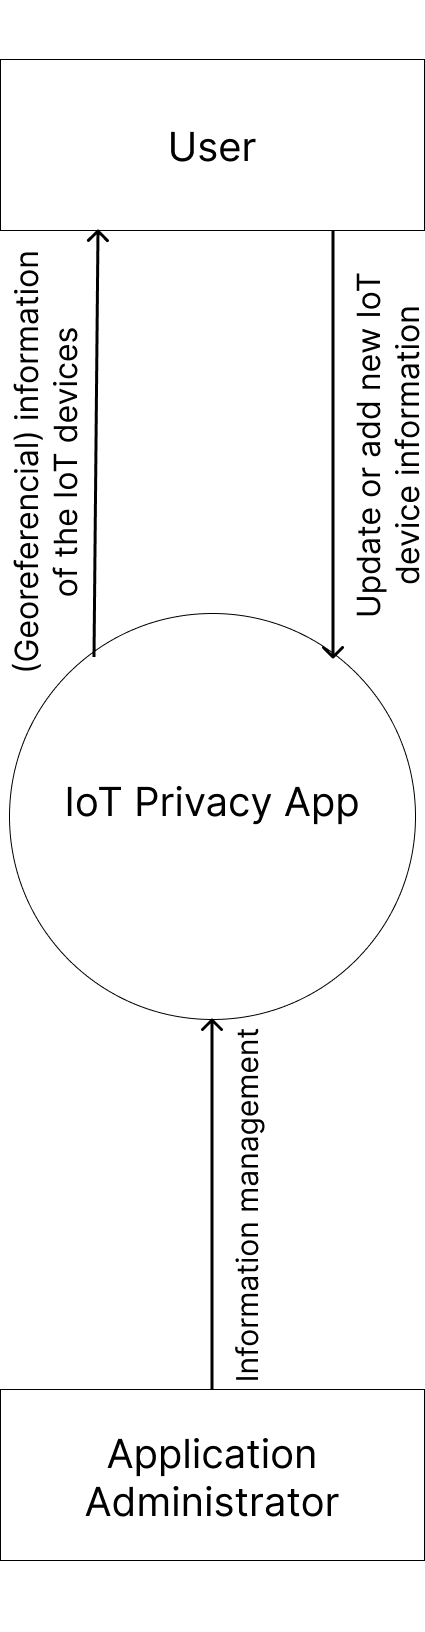
\includegraphics[width=3.5cm]{../app/docs/software_requirements/assets/images/contextual_diagram.png}
    \caption{Contextual diagram depicting the interaction between two stakeholders, the user and the administrator, and the application.}
    \label{fig:contextual diagram}
\end{figure}

The interaction links between the stakeholders and the application as represented
on the contextual diagram can be dissected as follows:\\
\newline
User: \\
\newline
→ Receives:

$\bullet$ (Georeferencial) information of the IoT devices\\
\newline
→ Sends:

$\bullet$ Update or addition of IoT device information\\
\newline
Application Administrator (Programmer): \\
\newline
→ Receives:

$\bullet$ All information related to the application\\
\newline
→ Sends:

$\bullet$ Information management

\subsubsection{Data Flow Diagram}

A data flow diagram shows how information flows between the various entities
in the system and their relationships.

\begin{figure}[H]
    \centering
    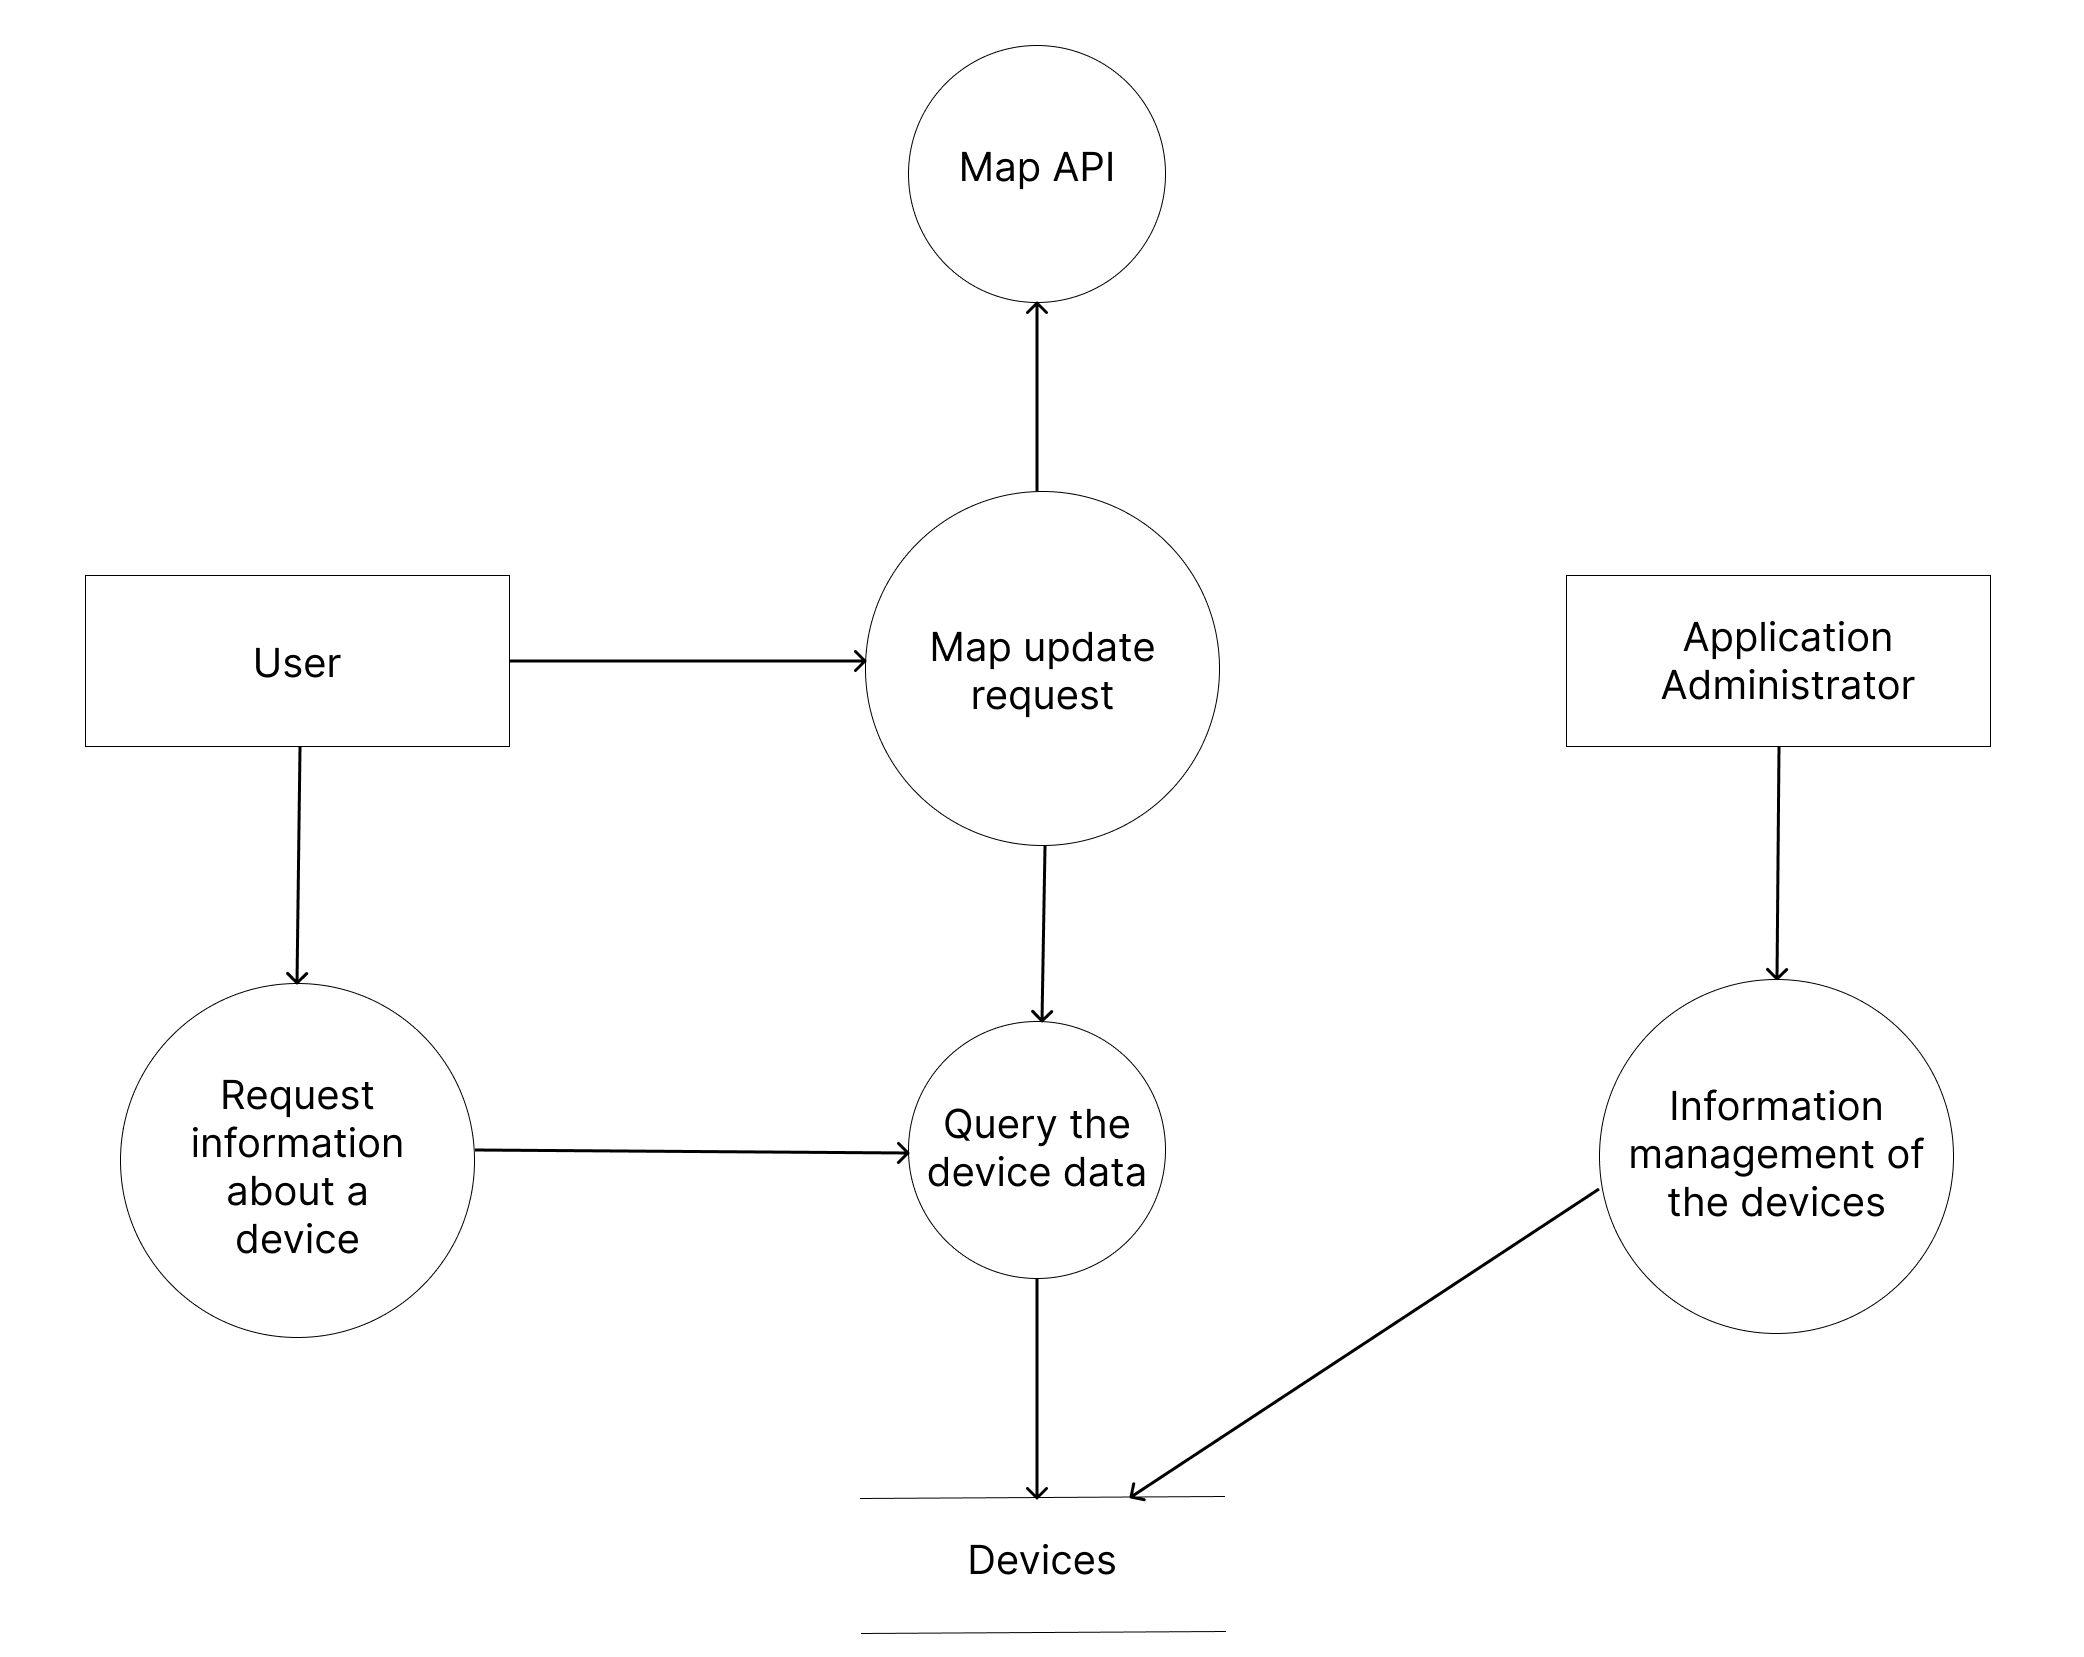
\includegraphics[width=15cm]{../app/docs/software_requirements/assets/images/data_flow_diagram.png}
    \caption{Data flow diagram.}
    \label{fig:data flow diagram}
\end{figure}

As shown on Figure \ref{fig:data flow diagram}, the user can browse the application
map, which will be interacted through an API,
and see the location of the IoT devices, the user can also look up information
about the devices by clicking on a device on the map or by searching for
the device in the application. The administrator of the application is responsible for
its maintenance by correcting or deleting incorrect data, implementing security
measures and for the stability and reliability of the system.

\subsubsection{Swimlane Diagram}

A swimlane diagram is a type of flowchart in which processes and decisions
are grouped into lanes. Parallel lines divide the diagram into lanes, each
lane being assigned to a stakeholder and the application.

\begin{figure}[H]
    \centering
    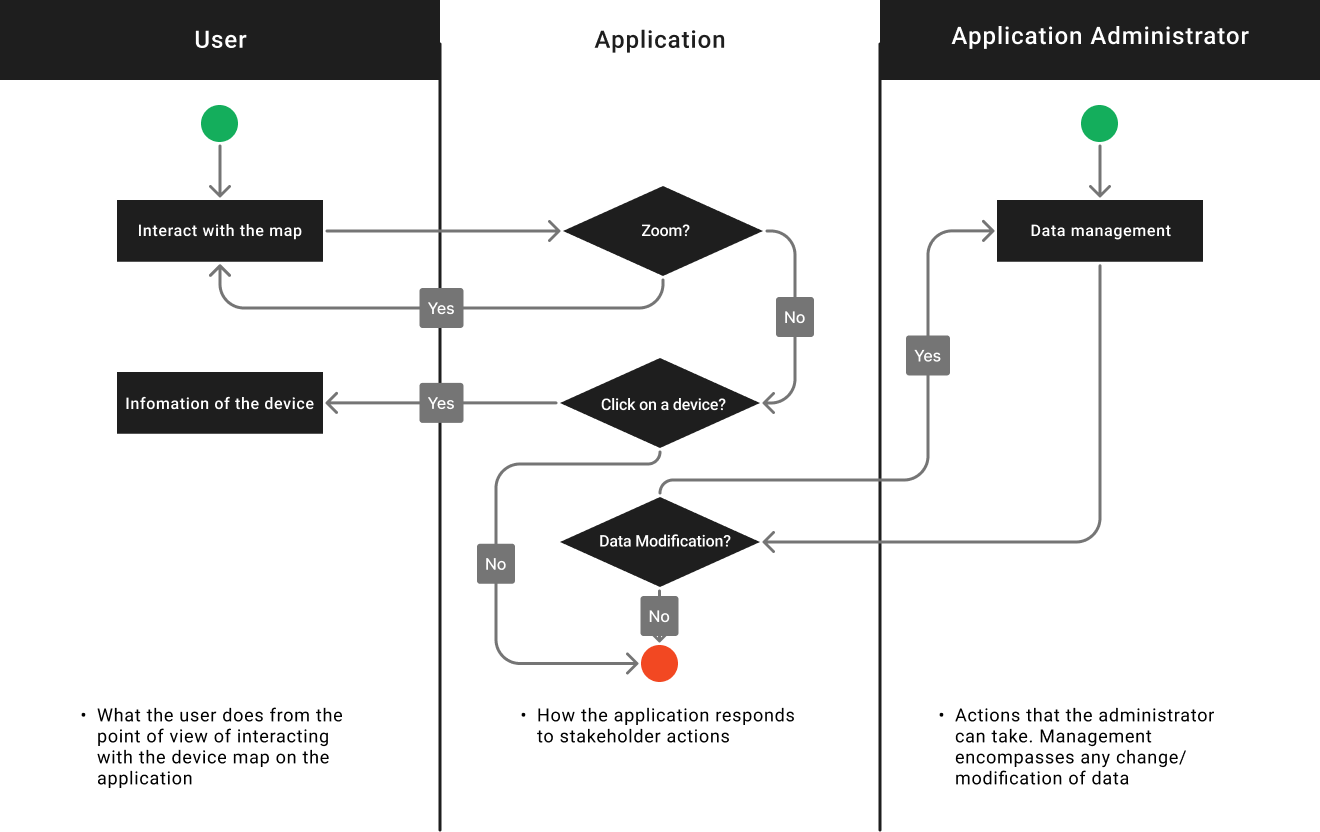
\includegraphics[width=15cm]{../app/docs/software_requirements/assets/images/swimlane_diagram.png}
    \caption{Swimlane diagram.}
    \label{fig:diagram swimlane}
\end{figure}

This swimlane diagram represents a high level view of a possible user interaction
from the application's map, on Figure \ref{fig:diagram swimlane} the user can view the location of
IoT devices and can see more information about a particular device by selecting
it on the map. The application administrator, as mentioned above, can modify the
devices' data.

\subsubsection{Business Requirements}

Business requirements describe in business terms what must be delivered
or achieved to deliver value. It is what defines the way of doing business,
reflecting the internal policy, the defined process and/or the basic rules
of conduct.  In other words, it is a set of instructions that users already
follow and that the system to be developed must contemplate. Restrictions,
validations, conditions and process exceptions are classic examples of business
rules. A business rule will not necessarily be reflected in the system as
a functionality, but it will certainly determine the behaviour of one or
more functionalities of the system.
\newline
No business requirements have been identified for this project.

\subsubsection{Technology Requirements}

Technology requirements describe what both hardware and software must be
used in order for a system to be realizable. In terms of hardware, it describes
what kind of physical components are needed for the software to work. The
software to be chosen must take into account the hardware that has been
chosen and what is intended by the stakeholders. This has implications for
how the system is implemented.
\newline
The technology requirements that have been identified for this project are as follows:
\begin{itemize}
    \item[$\bullet$] Firestore or similar database server
    \item[$\bullet$] Flutter framework with Dart being the main programming language
    \item[$\bullet$] Accessible on any smartphone (iOS or Android) \newline \textbf{Note}: No web based version is to be available.
\end{itemize}
These requirements have been chosen so that the system is available to as
many users as possible regardless of the hardware they use. The database
will allow to store the information that the users provide about the IoT
devices. The application will be developed with Flutter since it uses ahead
of time and just in time compilation with Dart as its programming language.
Flutter has better performance than React Native or a PWA stack and as such it is the chosen framework for
this application.

\subsubsection{Requirements Table}

The requirements table identifies each feature and links each feature to an origin
which can come from brainstorming sessions or interviews for example.
This is important as it makes to managing requirements in the future easier.
Knowing where the requirements came from makes it simpler to clarify any questions
and refer back to the original source.
\newline
Table \ref{table:table1} lists all the features that have been identified, for
each feature it was identified the stakeholders to which it applies, a description
of the feature and its source. There have been identified 10 features that will
compose the backbone of the application.

\begin{table}[H]
    \centering
    \begin{adjustbox}{width=1\textwidth,center=\textwidth}
    \begin{tabular}{|l|p{0.2\textwidth}|p{0.2\textwidth}|p{0.4\textwidth}|p{0.15\textwidth}|}
        \hline
        \rowcolor{blue!5}
        \textbf{R\#} & \textbf{Feature} & \textbf{Applicable stakeholders} & \textbf{Description} & \textbf{Source} \\
        \hline
        \textbf{1} & Navigate the map & User & \textbf{User}: The system should allow the user to scroll through the map of devices & Dissertation preparation \\
        \hline
        \textbf{2} & Select device on the map & User & \textbf{User}: The system should allow the user to select a device on the map to view more information & Dissertation preparation \\
        \hline
        \textbf{3} & Query devices through parameters & User & \textbf{User}: The system should allow the user to consult devices of only a certain type, data collected, general location & Dissertation preparation \\
        \hline
        \textbf{4} & Query statistics of the devices & User & \textbf{User}: The system should allow consulting statistics of devices & Dissertation preparation \\
        \hline
        \textbf{5} & Add a device & User & \textbf{User}: The system should allow the user to add a new device with name, category, data collected, location, etc. & Dissertation preparation \\
        \hline
        \textbf{6} & Edit a device & User & \textbf{User}: The system should allow the user to change some data of a device & Dissertation preparation \\
        \hline
        \textbf{7} & Delete a device & App Administrator & \textbf{App Administrator}: The system should allow the administrator to delete a device & Dissertation preparation \\
        \hline
        \textbf{8} & Create account & User & \textbf{User}: The system shall allow a user to create an account. & Dissertation preparation \\
        \hline
        \textbf{9} & Select privacy choices & User & \textbf{User}: The system shall allow the user to select their privacy choices for a certain device if the device allows for it. & Dissertation preparation \\
        \hline
        \textbf{10} & See more information about privacy in IoT & User & \textbf{User}: The system shall allow the user to check what the terms used in the application mean. & Survey results \\
        \hline
    \end{tabular}
    \end{adjustbox}
    \vspace{1em}
    \caption{Requirements table.}
    \label{table:table1}
\end{table}

\subsubsection{Functional Requirements}

Functional requirements \cite{fulton2017chapter} define the functions of a system or its components,
where functions are specifications or behaviours between system outputs and
inputs. These outline what developers must implement in order for users to
accomplish tasks, which then fulfil business requirements. Functional requirements are
essential to the success of a project.
After building the tracing table, the functional requirements that were needed
were extracted for each feature and grouped appropriately according to the
following groups:

\paragraph{User Requirements}

\textbf{UR1} - The system shall allow the user to navigate through the devices georeferences;
\newline
\textbf{UR2} - The system shall allow the user to select a device on the map to view more information;
\newline
\textbf{UR4} - The system shall allow the user to consult devices of only a certain category, data collected, etc.;
\newline
\textbf{UR5} - The system shall allow consulting statistics of the devices;
\newline
\textbf{UR6} - The system shall allow the user to create an account;
\newline
\textbf{UR7} - The system shall allow a logged in user to add a new device with name, category, data collected, location, etc.;
\newline
\textbf{UR8} - The system shall allow a logged in user to change associated data of a device;

\paragraph{Administrator Requirements}

\textbf{AR1} - The system shall allow a logged in administrator to add a new device with name, category, data collected, location, etc.;
\newline
\textbf{AR2} - The system shall allow a logged in administrator to change associated data of a device;
\newline
\textbf{AR3} - The system shall allow a logged in administrator to delete a device;

\paragraph{System Requirements}

\textbf{SR1} - The system shall generate statistics related to the IoT devices that reside in the database;

\subsubsection{Non-Functional Requirements}

\textbf{NFR1} - The system shall behave the same in different platforms (Android and iOS);

\subsubsection{Use Cases Diagram}

The use cases diagram \cite{wiegers2013software} provides a high level visualisation of the user
requirements. The box represents the system boundary. An actor's arrow
for a use case indicates that he is the primary actor for it.
The primary actor initiates the use case and derives the primary value
from it.

In Figure \ref{fig:use_cases_diagram}, it is possible to determine the use cases
that have been identified, based on the previously specified system requirements.
The use cases related to the user are: browsing the map, create an account, search for
a device, check device statistics, add and edit a device and consult information
about a specific device. Meanwhile the use cases for the application administrator are:
adding editing or deleting a device, although the administrator can do all other
tasks as a regular user.

\begin{figure}[H]
    \centering
    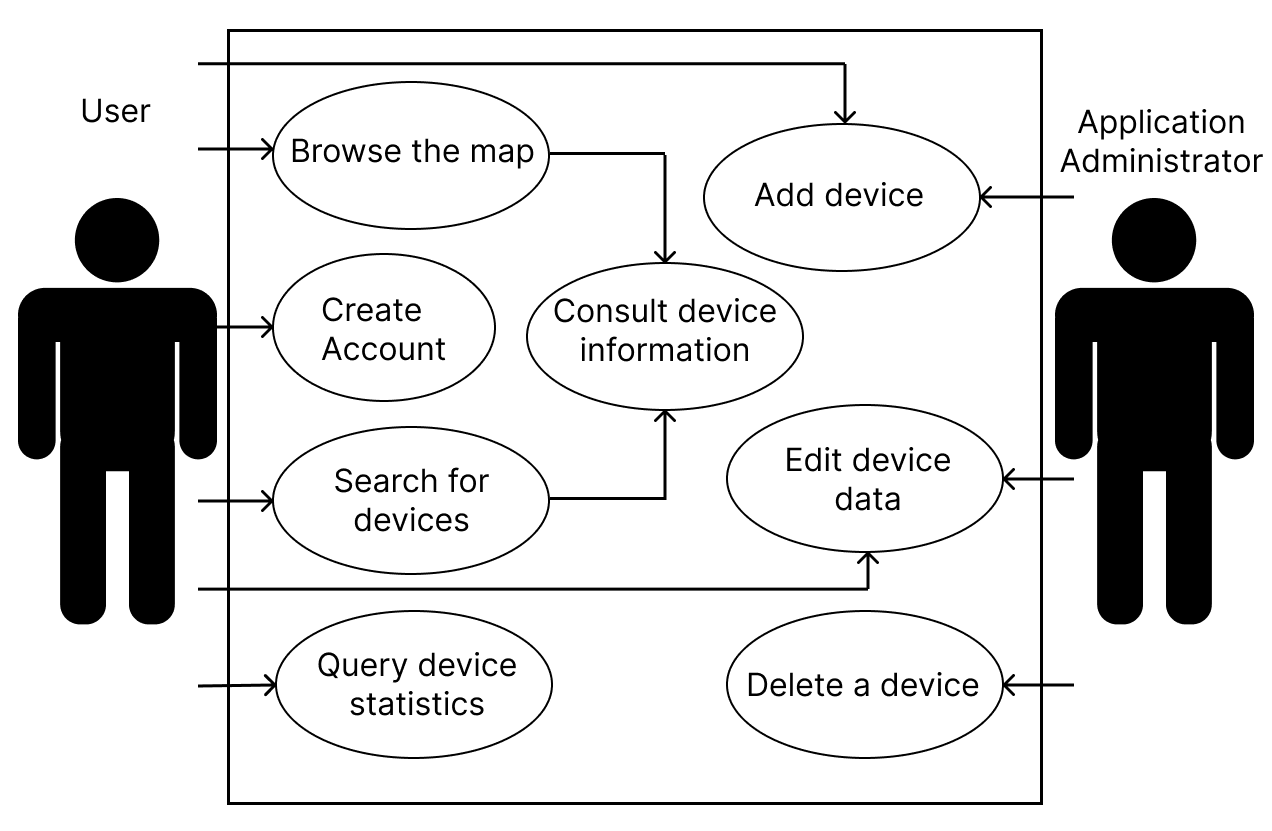
\includegraphics[width=15cm]{../app/docs/software_requirements/assets/images/use_cases_diagram.png}
    \caption{Use cases diagram.}
    \label{fig:use_cases_diagram}
\end{figure}

\subsubsection{Use Cases}

A use case is a type of classifier representing a
coherent functional unit provided by the system, subsystem, or class manifested
by sequences of interchangeable messages between systems and one or more
actors.

This technique describes the tasks that users need to perform with
the system or the user-system interaction that may be important to some
stakeholders. They also help in testing by checking that the functionality
has been implemented correctly. The use cases uses an Unified Modeling
Language (UML) notation.

Based on the use cases represented on Figure \ref{fig:use_cases_diagram},
use case ``Query devices through certain parameters'' has been detailed on Table \ref{table:use_case1};
use case ``Query device statistics'' has been detailed on Table \ref{table:use_case2};
use case ``Add a device'' has been detailed on Table \ref{table:use_case3};
use case ``Edit a device's data'' has been detailed on Table \ref{table:use_case4};
use case ``Delete a device'' has been detailed on Table \ref{table:use_case5};
and use case ``Create an account'' has been detailed on Table \ref{table:use_case6};

\begin{table}[H]
    \centering
    \begin{adjustbox}{width=1.2\textwidth,center=\textwidth}
        \begin{tabular}{|m{4cm}|m{12cm}|}
            \hline
            \textbf{ID and Name}: & UC-01 Query devices through certain parameters \\
            \hline
            \textbf{Created By}: & Nelson Vieira 20/02/2023 \\
            \hline
            \textbf{Primary Actor}: & End User \\
            \hline
            \textbf{Description}: & The user makes a device information query \\
            \hline
            \textbf{Trigger}: & The user wants to search device information \\
            \hline
            \textbf{Pre-conditions}: & N/A \\
            \hline
            \textbf{Post-conditions}: & POST-1. The user finds device information \\
            \hline
            \textbf{Normal Flow}: & \textbf{1.0 Query information of a device on the map}
            \begin{enumerate}
                \item The user browses the map
                \item The user clicks on the icon to show some information about the device
                \item The user clicks on the device pop-up
            \end{enumerate} \\
            \hline
            \textbf{Alternative Flow}: & \textbf{1.1 Device information search}
            \begin{enumerate}
                \item User enters device name
                \item The user chooses the device he wants from a list generated from the search performed
            \end{enumerate} \\
            \hline
            \textbf{Alternative Flow}: & \textbf{1.2 Alternative search for information from a device}
            \begin{enumerate}
                \item The user selects one of the parameters:
                \begin{enumerate}
                    \item Category
                    \item Name
                \end{enumerate}
                \item The user chooses the device he wants from a list generated from the search carried out
            \end{enumerate} \\
            \hline
            \textbf{Exceptions}: & \textbf{1.0.E1  The API is not working}
            \begin{enumerate}
                \item The system displays an alert message: ``We are having connection problems, please wait for a while''
            \end{enumerate} \\
            \hline
            \textbf{Priority}: & High \\
            \hline
            \textbf{Business Requirements}: & N/A \\
            \hline
            \textbf{Assumptions}: & N/A \\
            \hline
        \end{tabular}
    \end{adjustbox}
    \vspace{1em}
    \caption{Use case 1 - device information query.}
    \label{table:use_case1}
\end{table}

\begin{table}[H]
    \centering
    \begin{adjustbox}{width=1.2\textwidth,center=\textwidth}
        \begin{tabular}{|m{4cm}|m{12cm}|}
            \hline
            \textbf{ID and Name}: & UC-02 Device statistics query \\
            \hline
            \textbf{Created By}: & Nelson Vieira 20/02/2023 \\
            \hline
            \textbf{Primary Actor}: & End User \\
            \hline
            \textbf{Description}: & The user queries the statistics of the devices \\
            \hline
            \textbf{Trigger}: & The user wants to find statistics of devices \\
            \hline
            \textbf{Pre-conditions}: & N/A \\
            \hline
            \textbf{Post-conditions}: & POST-1. The system displays the statistics of the devices \\
            \hline
            \textbf{Normal Flow}: & \textbf{2.0 Device statistics query}
            \begin{enumerate}
                \item User selects statistics tab
                \item The user can only select certain parameters, such as:
                \begin{enumerate}
                    \item Category
                    \item Location
                \end{enumerate}
            \end{enumerate} \\
            \hline
            \textbf{Alternative Flow}: & N/A \\
            \hline
            \textbf{Exceptions}: & \textbf{2.0.E1  The API is not working}
            \begin{enumerate}
                \item The system displays an alert message: ``We are having connection problems, please wait for a while''
            \end{enumerate} \\
            \hline
            \textbf{Priority}: & Medium \\
            \hline
            \textbf{Business Requirements}: & N/A \\
            \hline
            \textbf{Assumptions}: & N/A \\
            \hline
        \end{tabular}
    \end{adjustbox}
    \vspace{1em}
    \caption{Use case 2 - statistics query.}
    \label{table:use_case2}
\end{table}

\begin{table}[H]
    \centering
    \begin{adjustbox}{width=1.15\textwidth,center=\textwidth}
        \begin{tabular}{|m{4cm}|m{12cm}|}
            \hline
            \textbf{ID and Name}: & UC-03 Add a device \\
            \hline
            \textbf{Created By}: & Nelson Vieira 22/02/2023 \\
            \hline
            \textbf{Primary Actor}: & End User \\
            \hline
            \textbf{Description}: & Addition of a new IoT device in the application \\
            \hline
            \textbf{Trigger}: & The user wants to add a new IoT device \\
            \hline
            \textbf{Pre-conditions}: & N/A \\
            \hline
            \textbf{Post-conditions}: & POST-1. A new IoT device is added to the application \\
            \hline
            \textbf{Normal Flow}: & \textbf{3.0 Add a device}
            \begin{enumerate}
                \item The user enters the following data of a new IoT device:
                \begin{enumerate}
                    \item Name
                    \item Type of data collected
                    \item Category
                    \item Photos
                \end{enumerate}
                \item The user clicks submit
                \item The user adds the location of the IoT device on the map
            \end{enumerate} \\
            \hline
            \textbf{Alternative Flow}: & N/A \\
            \hline
            \textbf{Exceptions}: & \textbf{3.0.E1  The device is already in the database}
            \begin{enumerate}
                \item The system displays an error message
            \end{enumerate} \\
            \hline
            \textbf{Priority}: & High \\
            \hline
            \textbf{Business Requirements}: & N/A \\
            \hline
            \textbf{Assumptions}: & N/A \\
            \hline
        \end{tabular}
    \end{adjustbox}
    \vspace{1em}
    \caption{Use case 3 - add a device.}
    \label{table:use_case3}
\end{table}

\begin{table}[H]
    \centering
    \begin{adjustbox}{width=1.1\textwidth,center=\textwidth}
        \begin{tabular}{|m{4cm}|m{12cm}|}
            \hline
            \textbf{ID and Name}: & UC-04 Edit a device's data \\
            \hline
            \textbf{Created By}: & Nelson Vieira 22/02/2023 \\
            \hline
            \textbf{Primary Actor}: & End User \\
            \hline
            \textbf{Description}: & Editing the data of an IoT device in the application \\
            \hline
            \textbf{Trigger}: & The user wants to edit an IoT device's data \\
            \hline
            \textbf{Pre-conditions}: & N/A \\
            \hline
            \textbf{Post-conditions}: & POST-1. The data that has been changed appears in the application \\
            \hline
            \textbf{Normal Flow}: & \textbf{4.0 Edit a device's data}
            \begin{enumerate}
                \item The user can change any of the following device data:
                \begin{enumerate}
                    \item Name
                    \item Category
                    \item Photos
                \end{enumerate}
                \item The user clicks on submit
            \end{enumerate} \\
            \hline
            \textbf{Alternative Flow}: & N/A \\
            \hline
            \textbf{Exceptions}: &
            % Exceptions: & \textbf{4.0.E1  Unique data already registered}
            % \begin{enumerate}
            %     \item The system displays an error message
            %     \item The system asks the user to enter different data
            % \end{enumerate}
            \textbf{4.0.E1  The device to be edited has been deleted in the meantime}
            \begin{enumerate}
                \item The system displays an error message
                \item The system prohibits editing
            \end{enumerate} \\
            \hline
            \textbf{Priority}: & High \\
            \hline
            \textbf{Business Requirements}: & N/A \\
            \hline
            \textbf{Assumptions}: & N/A \\
            \hline
        \end{tabular}
    \end{adjustbox}
    \vspace{1em}
    \caption{Use case 4 - edit a device's data.}
    \label{table:use_case4}
\end{table}

\begin{table}[H]
    \centering
    \begin{adjustbox}{width=1.2\textwidth,center=\textwidth}
        \begin{tabular}{|m{4cm}|m{12cm}|}
            \hline
            \textbf{ID and Name}: & UC-05 Delete a device \\
            \hline
            \textbf{Created By}: & Nelson Vieira 22/02/2023 \\
            \hline
            \textbf{Primary Actor}: & App Administrator \\
            \hline
            \textbf{Description}: & Deleting a device in the application \\
            \hline
            \textbf{Trigger}: & The administrator wants to delete a device \\
            \hline
            \textbf{Pre-conditions}: & PRE-1. The device to be deleted must be in the application's database \\
            \hline
            \textbf{Post-conditions}: & POST-1. The device is deleted from the application \\
            \hline
            \textbf{Normal Flow}: & \textbf{5.0 Delete a device}
            \begin{enumerate}
                \item The administrator deletes a device, through:
                \begin{enumerate}
                    \item ID of device
                    \item Name of device
                \end{enumerate}
                \item The administrator confirms the deletion
                \item The system deletes the device
            \end{enumerate} \\
            \hline
            \textbf{Alternative Flow}: & N/A \\
            \hline
            \textbf{Exceptions}: & \textbf{5.0.E1  The device to be deleted no longer exists in the database}
            \begin{enumerate}
                \item The system displays an error message
                \item The system prohibits deletion
            \end{enumerate} \\
            \hline
            \textbf{Priority}: & High \\
            \hline
            \textbf{Business Requirements}: & N/A \\
            \hline
            \textbf{Assumptions}: & It is assumed that the administrator has database access \\
            \hline
        \end{tabular}
    \end{adjustbox}
    \vspace{1em}
    \caption{Use case 5 - delete a device.}
    \label{table:use_case5}
\end{table}

\begin{table}[H]
    \centering
    \begin{adjustbox}{width=1.2\textwidth,center=\textwidth}
        \begin{tabular}{|m{4cm}|m{12cm}|}
            \hline
            \textbf{ID and Name}: & UC-06 Create an account \\
            \hline
            \textbf{Created By}: & Nelson Vieira 22/02/2023 \\
            \hline
            \textbf{Primary Actor}: & End User \\
            \hline
            \textbf{Description}: & Create a new end user account \\
            \hline
            \textbf{Trigger}: & The user wants to create an account \\
            \hline
            \textbf{Pre-conditions}: & PRE-1. The user wants to add a new device \\
            \hline
            \textbf{Post-conditions}: & POST-1. The account is created in the application \\
            \hline
            \textbf{Normal Flow}: & \textbf{6.0 Account creation process}
            \begin{enumerate}
                \item The user enter the following data in the register screen:
                \begin{enumerate}
                    \item Username
                    \item Email
                    \item Password
                \end{enumerate}
                \item The system adds the account data to the database
                \item An account confirmation email is sent to the email provided by the user
                \item The user confirms the account
            \end{enumerate} \\
            \hline
            \textbf{Alternative Flow}: & N/A \\
            \hline
            \textbf{Exceptions}: & \textbf{6.0.E1  The username already exists in the database}
            \begin{enumerate}
                \item The system displays an error message
                \item The system allows the user to recover the account
            \end{enumerate}
            \textbf{6.0.E2 The email already exists in the database}
            \begin{enumerate}
                \item The system displays an error message
                \item The system allows the user to recover the account
            \end{enumerate} \\
            \hline
            \textbf{Priority}: & High \\
            \hline
            \textbf{Business Requirements}: & N/A \\
            \hline
            \textbf{Assumptions}: & N/A \\
            \hline
        \end{tabular}
    \end{adjustbox}
    \vspace{1em}
    \caption{Use case 6 - create an account.}
    \label{table:use_case6}
\end{table}

\subsubsection{Requirements Prioritisation}

Regarding the prioritization of requirements, the Quality Function Deployment technique
proposed by Cohen in 1995 \cite{cohen1995quality} is used to estimate the priority of a group of requirements.
This is based on the benefit of including a feature/requirement, the penalty of not including
it, and also the cost and risks associated with implementation. By using the MoSCoW method \cite{clegg1994case} the
initial features are reduced to facilitate the use of the Quality Function Deployment table.

In this approach, Table \ref{table:tabela moscow}, the values 0 and 1 are used. In case of 1 it means that the column requirement/feature
is a higher priority than the row one and if it is 0 the opposite is true.

\begin{table}[H]
    \centering
    \begin{adjustbox}{width=0.8\textwidth,center=\textwidth}
        \begin{tabular}{|>{\columncolor{gray!5!white}}r|r|r|r|r|r|r|r|r|r|r|}
            \hline
            \rowcolor{gray!5!white}
            & \textbf{R\#1} & \textbf{R\#2} & \textbf{R\#3} & \textbf{R\#4} & \textbf{R\#5} & \textbf{R\#6} & \textbf{R\#7} & \textbf{R\#8} & \textbf{R\#9} & \textbf{R\#10} \\
            \hline
            \textbf{R\#1} && 0 & 0 & 0 & 1 & 0 & 0 & 0 & 0 & 0 \\
            \hline
            \textbf{R\#2} & 1 && 0 & 0 & 1 & 0 & 0 & 0 & 0 & 0 \\
            \hline
            \textbf{R\#3} & 1 & 1 && 0 & 1 & 0 & 0 & 0 & 0 & 0 \\
            \hline
            \textbf{R\#4} & 1 & 1 & 1 && 1 & 0 & 0 & 0 & 1 & 1 \\
            \hline
            \textbf{R\#5} & 0 & 0 & 0 & 0 && 0 & 0 & 1 & 1 & 1 \\
            \hline
            \textbf{R\#6} & 1 & 1 & 1 & 1 & 1 && 0 & 0 & 1 & 1 \\
            \hline
            \textbf{R\#7} & 1 & 1 & 1 & 1 & 1 & 1 && 1 & 1 & 1 \\
            \hline
            \textbf{R\#8} & 1 & 1 & 1 & 1 & 0 & 1 & 0 && 1 & 1 \\
            \hline
            \textbf{R\#9} & 1 & 1 & 1 & 0 & 0 & 0 & 0 & 0 && 1 \\
            \hline
            \textbf{R\#10} & 1 & 1 & 1 & 0 & 0 & 0 & 0 & 0 & 0 & \\
            \hline
            \rowcolor{gray!20}
            \textbf{Total} & 8 & 7 & 6 & 3 & 6 & 2 & 0 & 2 & 5 & 6 \\
            \hline
        \end{tabular}
    \end{adjustbox}
    \vspace{1em}
    \caption{Prioritisation table using the MoSCoW technique.}
    \label{table:tabela moscow}
\end{table}

After this initial selection, the prioritisation of requirements was estimated, as shown on Table \ref{table:prioritisation table},
where it is ranked, on a scale of 1 to 9, the benefit and penalty
of each requirement. The cost and implementation risk associated to each feature is
also estimated.

\begin{table}[H]
    \centering
    \begin{adjustbox}{width=1.2\textwidth,center=\textwidth}
    \begin{tabular}{|>{\columncolor{gray!10!white}}r|r|r|r|r|r|r|r|r|r|r|}
        \hline
        \rowcolor{gray!10!white}
        \multicolumn{2}{|c|}{\textbf{Feature}} & \textbf{Relative benefit} & \textbf{Relative penalty} & \textbf{Total value} & \textbf{Value \%} & \textbf{Relative cost} & \textbf{Cost \%} & \textbf{Relative risk} & \textbf{Risk \%} & \textbf{Priority} \\
        \hline
        Navigate the map & 1 & 9 & 9 & 27 & 13,24 & 5 & 10,42 & 5 & 10,00 & 0,65 \\
        \hline
        Select device on the map & 2 & 9 & 9 & 27 & 13,24 & 5 & 10,42 & 5 & 10,00 & 0,65 \\
        \hline
        Add a device & 5 & 9 & 9 & 27 & 13,24 & 3 & 6,25 & 4 & 8,00 & 0,93 \\
        \hline
        See more information about privacy in IoT & 10 & 5 & 6 & 24 & 11,76 & 6 & 12,50 & 2 & 4,00 & 0,71 \\
        \hline
        Query devices through parameters & 3 & 6 & 8 & 20 & 9,80 & 7 & 14,58 & 6 & 12,00 & 0,37 \\
        \hline
        Select privacy choices & 9 & 5 & 7 & 19 & 9,31 & 6 & 12,50 & 8 & 16,00 & 0,33 \\
        \hline
        Query statistics of the devices & 4 & 3 & 5 & 11 & 5,39 & 5 & 10,42 & 7 & 14,00 & 0,22 \\
        \hline
        Create account & 8 & 8 & 9 & 15 & 7,35 & 5 & 10,42 & 5 & 10,00 & 0,36 \\
        \hline
        Edit a device & 6 & 7 & 8 & 22 & 10,78 & 3 & 6,25 & 4 & 8,00 & 0,76 \\
        \hline
        Delete a device & 7 & 4 & 4 & 12 & 5,88 & 3 & 6,25 & 4 & 8,00 & 0,41 \\
        \hline
        \rowcolor{gray!50}
        \multicolumn{2}{|c|}{\textbf{Total}} & 67 & 62 & \textbf{198} & 100,00 & \textbf{39} & 100,00 & \textbf{37} & 100,00 & \\
        \hline
    \end{tabular}
    \end{adjustbox}
    \vspace{1em}
    \caption{Features prioritisation table.}
    \label{table:prioritisation table}
\end{table}

Using this method it is possible to get the requirements sorted by priority,
as seen on Table \ref{table:sorted requirements}.

\begin{table}[H]
    \centering
    \begin{adjustbox}{width=0.8\textwidth,center=\textwidth}
        \begin{tabular}{|c|c|c|c|}
            \hline
            \rowcolor{gray!5}
            \textbf{Rank} & \textbf{Feature} & \textbf{\# Feature} & \textbf{Priority} \\
            \hline
            1 & Add a device & 5 & 0,93 \\
            \hline
            2 & Edit a device & 6 & 0,76 \\
            \hline
            3 & See more information about privacy in IoT & 10 & 0,71 \\
            \hline
            4 & Navigate the map & 1 & 0,65 \\
            \hline
            5 & Select device on the map & 2 & 0,65 \\
            \hline
            6 & Delete a device & 7 & 0,41 \\
            \hline
            7 & Query devices through parameters & 3 & 0,37 \\
            \hline
            8 & Create an account & 8 & 0,36 \\
            \hline
            9 & Select privacy choices & 9 & 0,33 \\
            \hline
            10 & Query statistics of the devices & 4 & 0,22 \\
            \hline
        \end{tabular}
    \end{adjustbox}
    \vspace{1em}
    \caption{Highest priority requirements ordered.}
    \label{table:sorted requirements}
\end{table}

\subsubsection{Acceptance Criteria}

To make it easier to test whether the highest priority features that were chosen
previously were well implemented, these acceptance criteria were created for each
of them. These criteria help us understand the minimum conditions for this
application to be considered an MVP, i.e., for this project to have the minimum
possible requirements in order for it to be considered production ready.
\newline
For these acceptance criteria, the following was considered:

\begin{itemize}
    \item[$\bullet$] High-level functionality that must be present for the system to be usable
    \item[$\bullet$] Non-functional criteria and quality metrics that have to be satisfied
    \item[$\bullet$] Possibility of open problems or defects (we can guarantee that no defects or TBD is present for the system to be accepted)
    \item[$\bullet$] Legal or contractual restrictions (that have to be met for the system to be accepted)
\end{itemize}

\paragraph{Features}

\begin{itemize}
    \item[$\bullet$] Add a device
        \begin{itemize}
            \item[$\circ$] The system allows the user to add a new device that is not yet present in the database
        \end{itemize}
    \item[$\bullet$] Edit a device
    \begin{itemize}
        \item[$\circ$] The system allows the editing of an existing device
        \item[$\circ$] The system saves in the database the changes that have been made
    \end{itemize}
    \item[$\bullet$] Delete a device
    \begin{itemize}
        \item[$\circ$] The system allows the deletion of an existing device
        \item[$\circ$] The system deletes the device from its database
    \end{itemize}
    \item[$\bullet$] Navigate the map
    \begin{itemize}
        \item[$\circ$] The system can represent the devices on the map
        \item[$\circ$] The system allows the user to navigate throughout the map and view the devices
    \end{itemize}
    \item[$\bullet$] Query devices through parameters
    \begin{itemize}
        \item[$\circ$] The system allows searching devices by the certain parameters like the category, the type of data collected
    \end{itemize}
    \item[$\bullet$] Select device on map
    \begin{itemize}
        \item[$\circ$] The system allows the user to select a device on the map
    \end{itemize}
    \item[$\bullet$] See more information about privacy in IoT
    \begin{itemize}
        \item[$\circ$] The system allows the user to see more information about privacy in IoT
    \end{itemize}
    \item[$\bullet$] Select privacy choices
    \begin{itemize}
        \item[$\circ$] The system allows the user to select a device and view its details
        \item[$\circ$] The system allows the user to select privacy choices for that device (if that option is available)
    \end{itemize}
    \item[$\bullet$] Consult devices' statistics
    \begin{itemize}
        \item[$\circ$] The system allows the user to consult statistics concerning the devices
    \end{itemize}
    \item[$\bullet$] Create account
    \begin{itemize}
        \item[$\circ$] The system allows the creation of an account
        \item[$\circ$] The user has to enter its username, email and a password
        \item[$\circ$] The system can detect whether the email is already in use
        \item[$\circ$] The system can send a profile creation confirmation email
        \item[$\circ$] The user can confirm the profile creation
        \item[$\circ$] The system allows the user to sign in
    \end{itemize}
\end{itemize}

\subsection{Prototype}

After creating the software requirements specification, the prototypes were
created. For the creation of the prototypes the following tools were used: Figma
and GIMP. Figma was the primary tool for the design while GIMP was mostly used
for image manipulation as it is a more specialized software tool.

At first a low level prototype was made in order to understand the
general design and user interaction of the application. Figure \ref{fig:lowlevelprototype}
shows tree pages of the low level prototype, these being the homepage, about
and faq pages. This is a rough sketch, there are barely any details added to each page,
this only serves to get a general idea of where icons and other items
will be placed and how the navigation between screens will work.

\begin{figure}
    \centering
    \begin{subfigure}{0.33\textwidth}
        \centering
        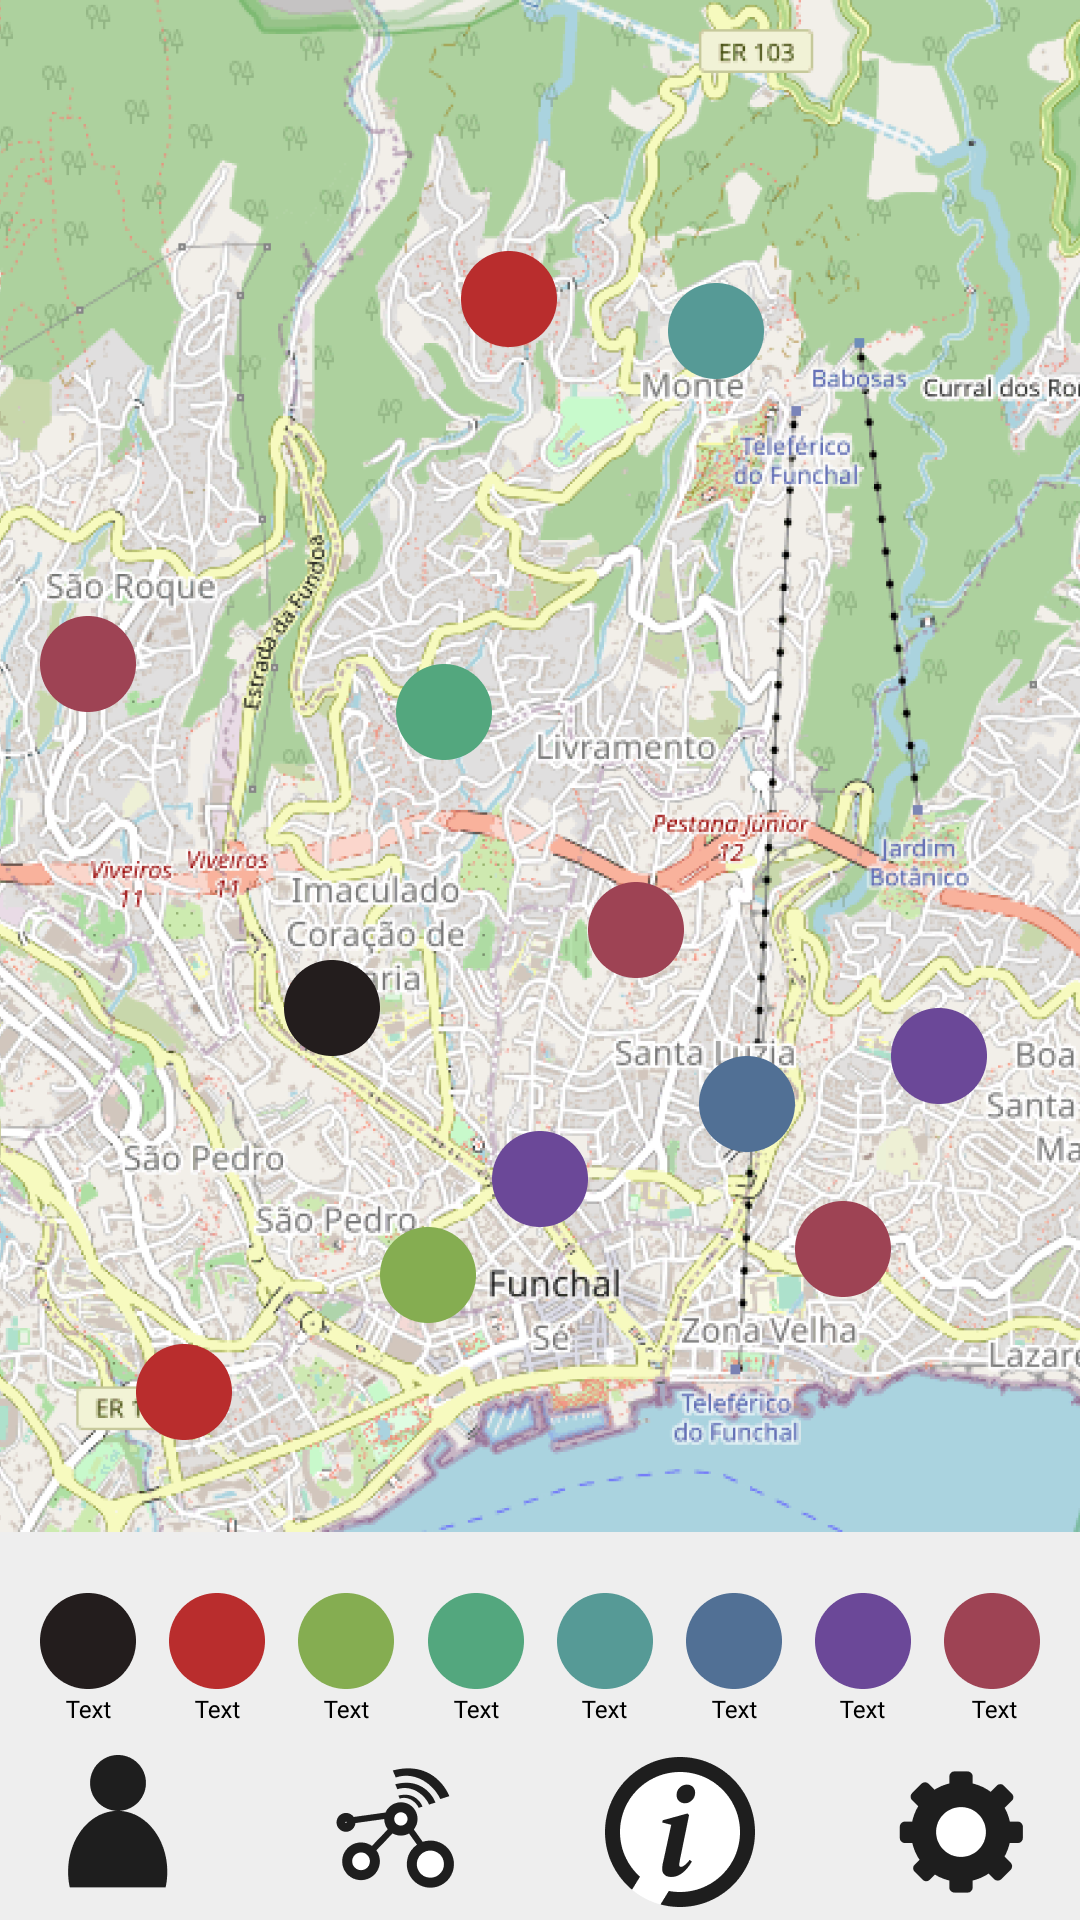
\includegraphics[width=130pt]{../assets/images/low_homepage.png}
        \caption{}
        \label{fig:lowhome}
    \end{subfigure}%
    \begin{subfigure}{0.33\textwidth}
        \centering
        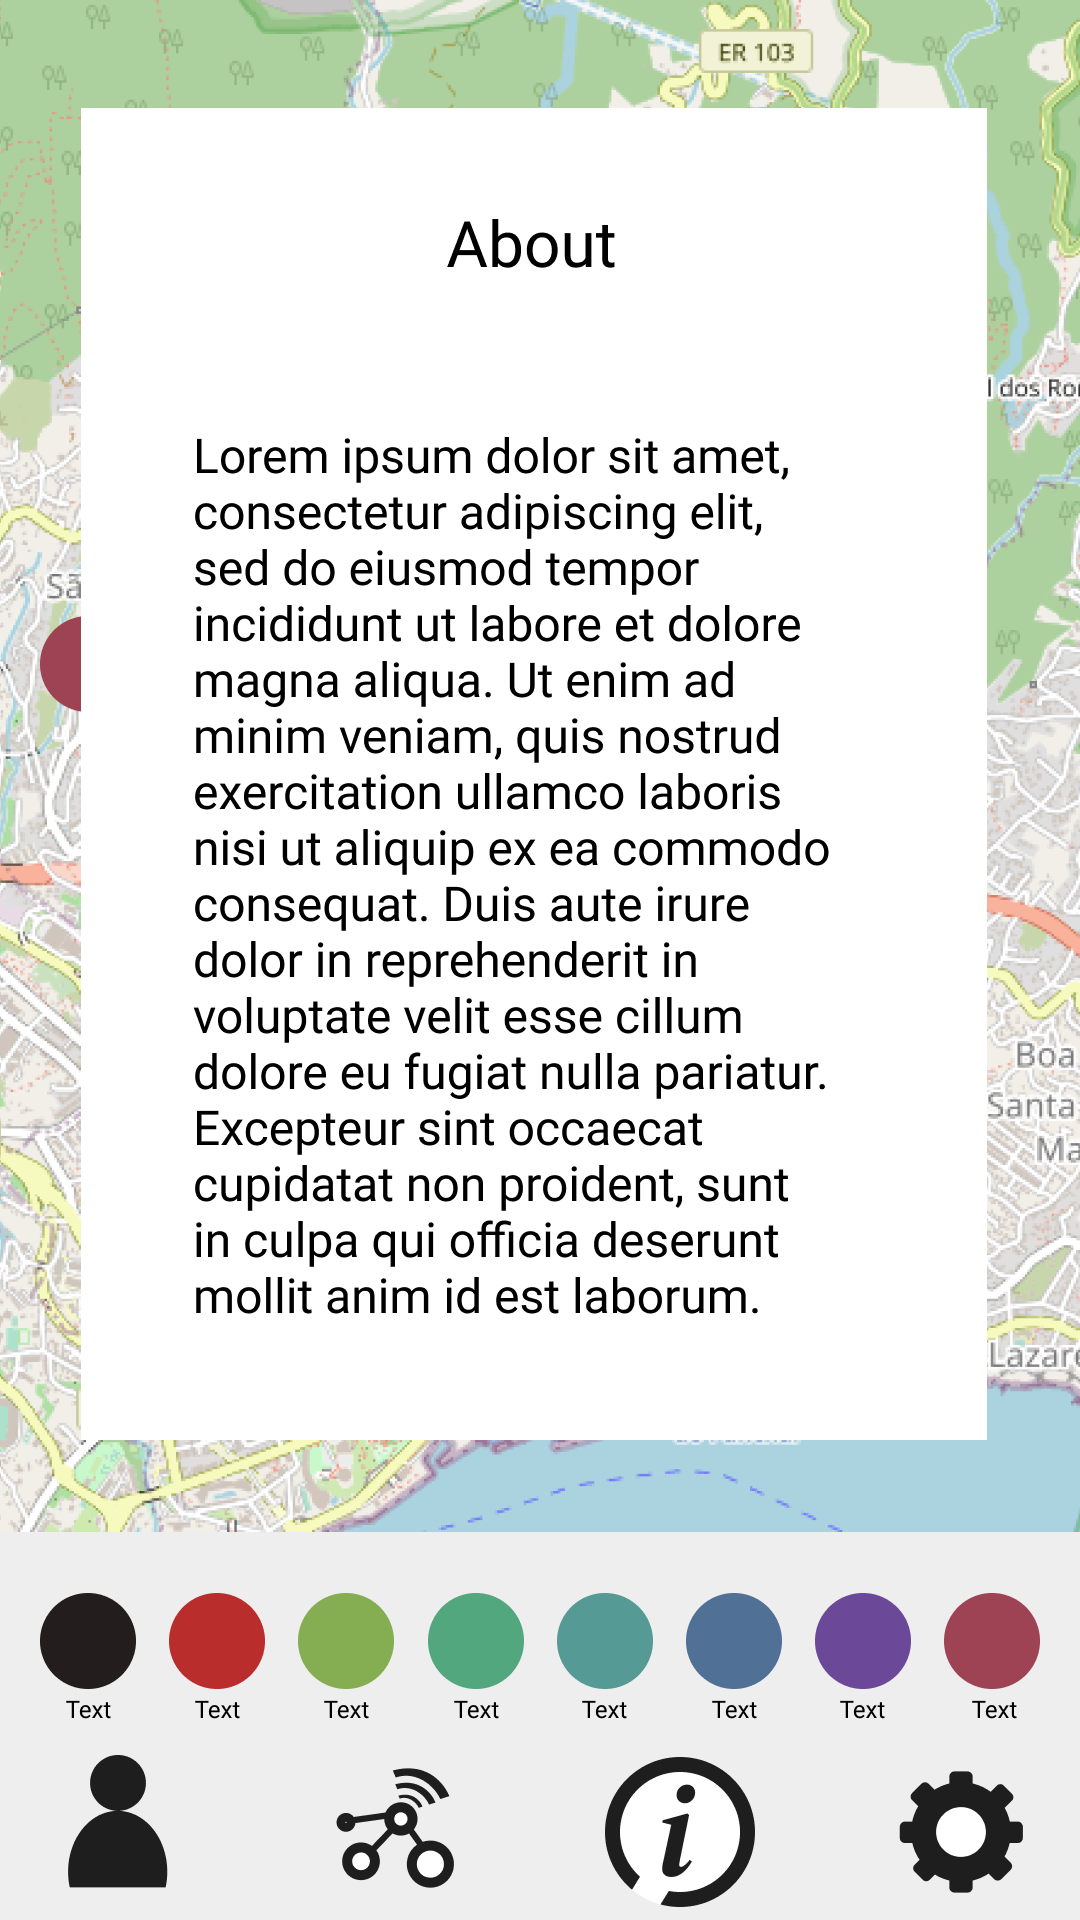
\includegraphics[width=130pt]{../assets/images/low_about.png}
        \caption{}
        \label{fig:lowabout}
    \end{subfigure}%
    \begin{subfigure}{0.33\textwidth}
        \centering
        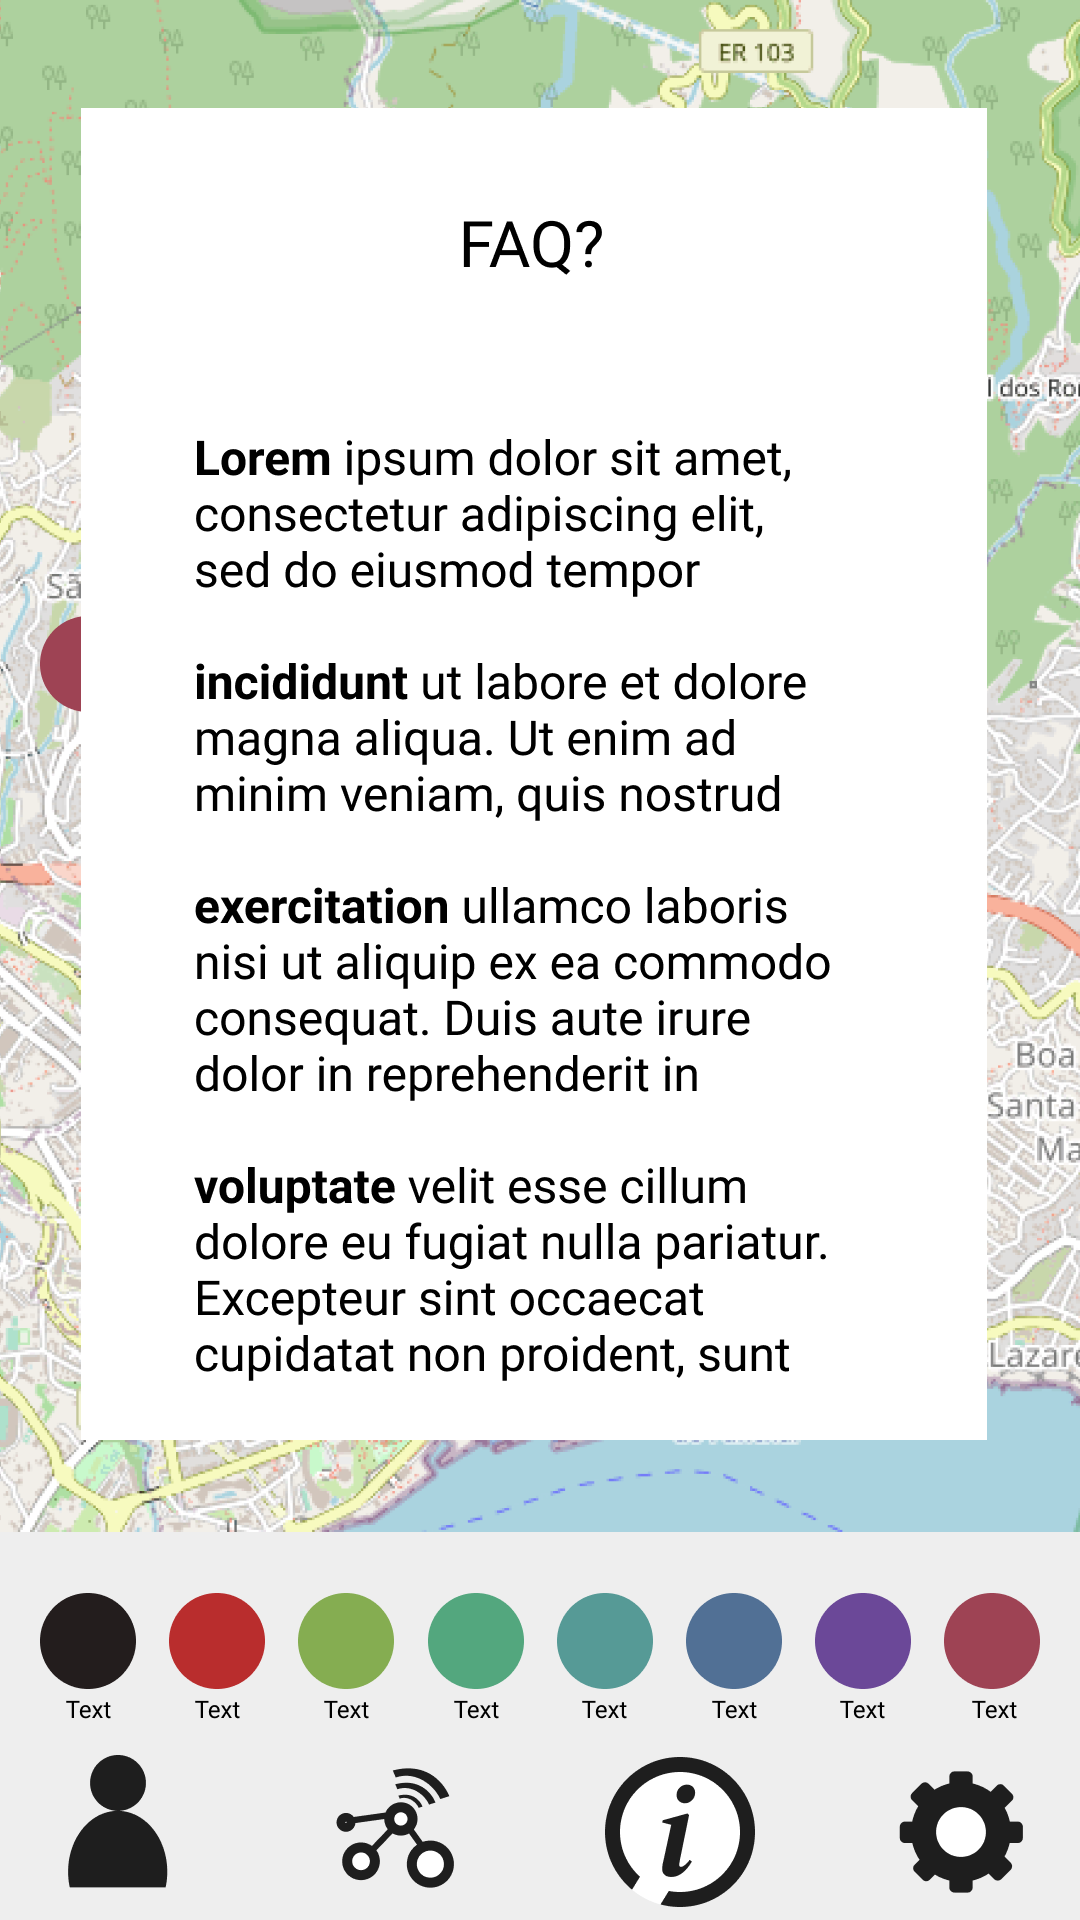
\includegraphics[width=130pt]{../assets/images/low_more_info.png}
        \caption{}
        \label{fig:lowfaq}
    \end{subfigure}%
    \caption{Low level prototype of (a) homepage, (b) about and (c) FAQ pages.}
    \label{fig:lowlevelprototype}
\end{figure}

After doing a rough prototype, some refinements were done to each page, like
adding colours and creating icons, which became eventually became a medium level
prototype. Figure \ref{fig:mediumlevelprototype} shows tree pages of the medium level
prototype, these being the homepage, about
and faq pages. This prototype has a navigation menu on the bottom where the
other pages of the application can be selected along with some information
above the page icons, this information is supposed to be the categories of
the devices, the logic would be that the user could tap one of these categories
and only devices of that category should be displayed on the map. It can
be seen that between the three pages the map stays in the background and
the various pages work like an overlay on the homepage, this would be
changed in subsequent prototype versions.

\begin{figure}
    \centering
    \begin{subfigure}{0.33\textwidth}
        \centering
        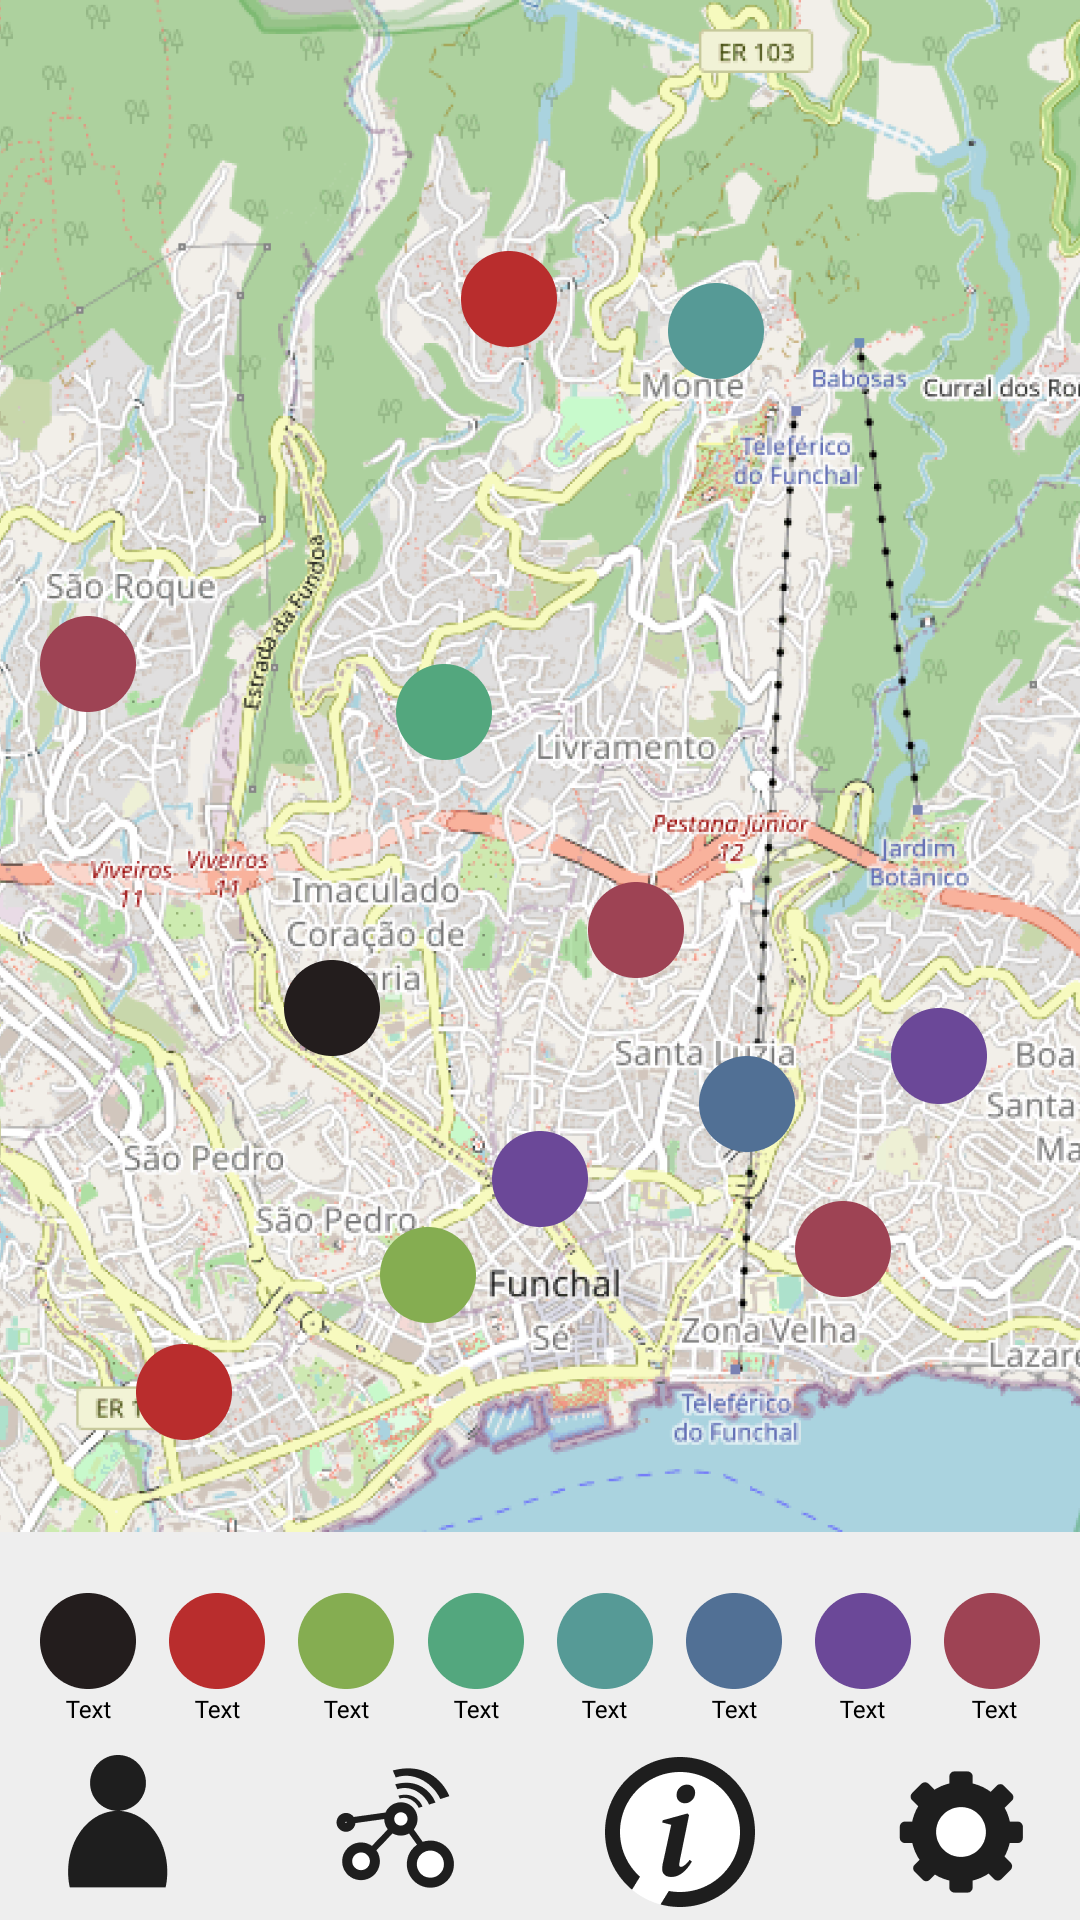
\includegraphics[width=130pt]{../assets/images/medium_homepage.png}
        \caption{}
        \label{fig:mediumhome}
    \end{subfigure}%
    \begin{subfigure}{0.33\textwidth}
        \centering
        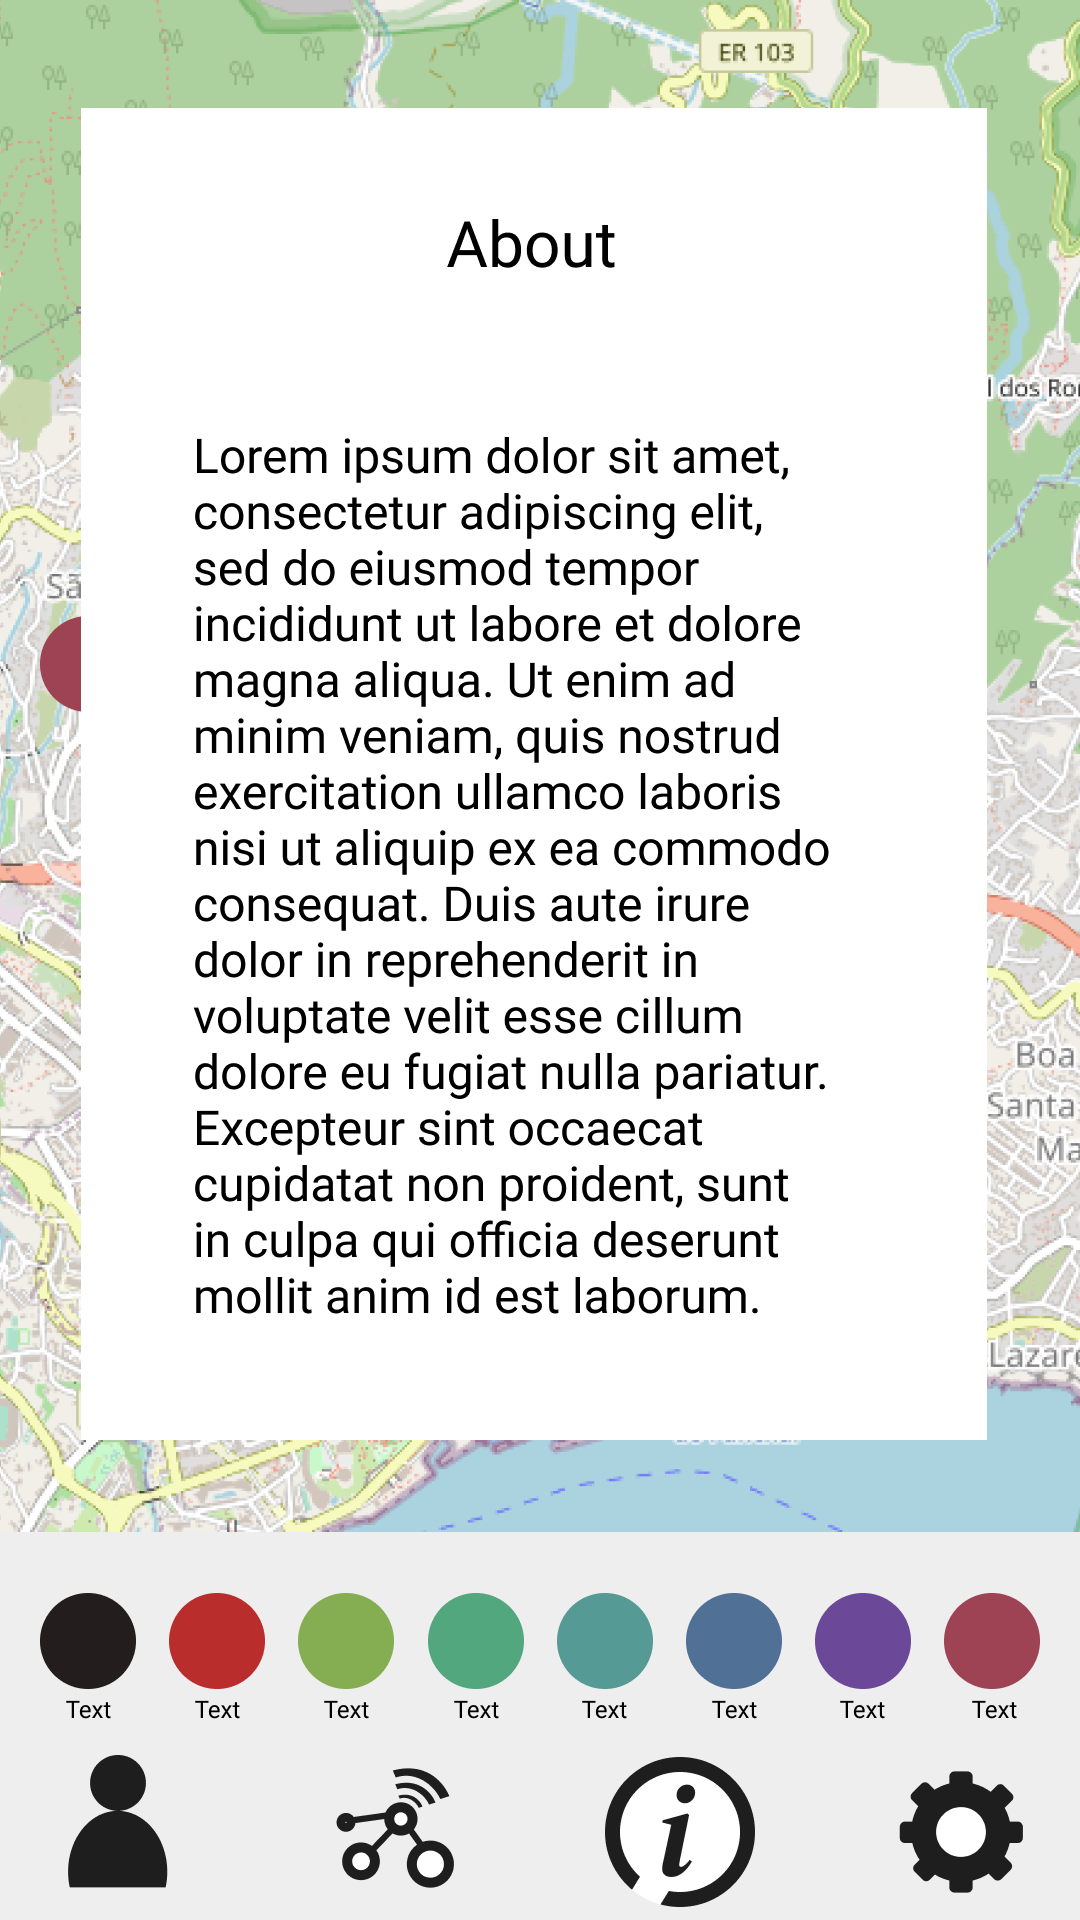
\includegraphics[width=130pt]{../assets/images/medium_about.png}
        \caption{}
        \label{fig:mediumabout}
    \end{subfigure}%
    \begin{subfigure}{0.33\textwidth}
        \centering
        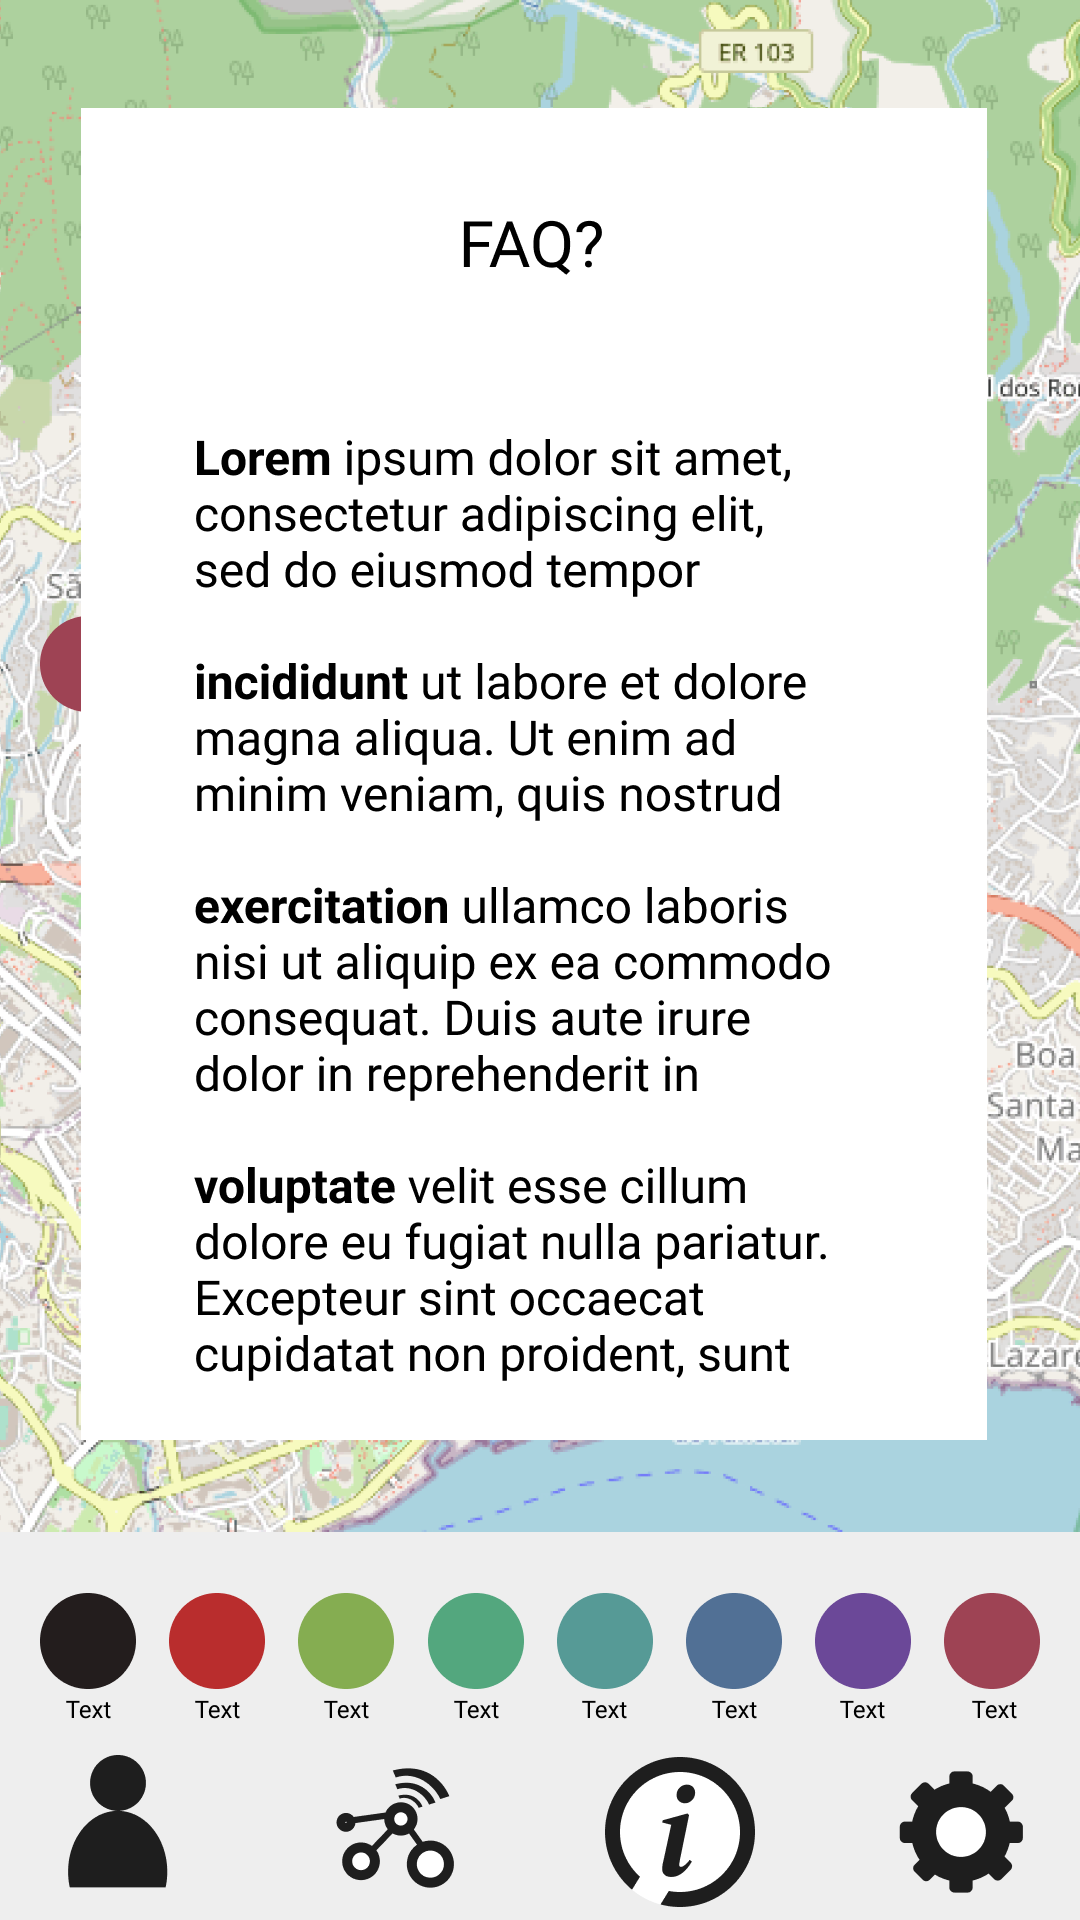
\includegraphics[width=130pt]{../assets/images/medium_more_info.png}
        \caption{}
        \label{fig:mediumfaq}
    \end{subfigure}%
    \caption{Medium level prototype of (a) homepage, (b) about and (c) FAQ pages.}
    \label{fig:mediumlevelprototype}
\end{figure}

Another prototype version was created, this being the final one before
the developed version. The high level version can be seen on Figure \ref{fig:highlevelprototype}
which shows three pages: homepage, FAQ and IoT devices. This is the version
that more closely resembles the developed application, although some design
elements were changed. Between the medium and high level prototypes, more icons
were created, colours were changed and other pages were designed. More icons
to the navigation footer were created, namely for the homepage and faq pages
which were missing from previous versions even with those pages being designed.
An icon for each category was also created, these show up on the map, representing
the type of device, and also on the devices page, so that devices can be quickly
identified.

\begin{figure}[H]
    \centering
    \begin{subfigure}{0.33\textwidth}
        \centering
        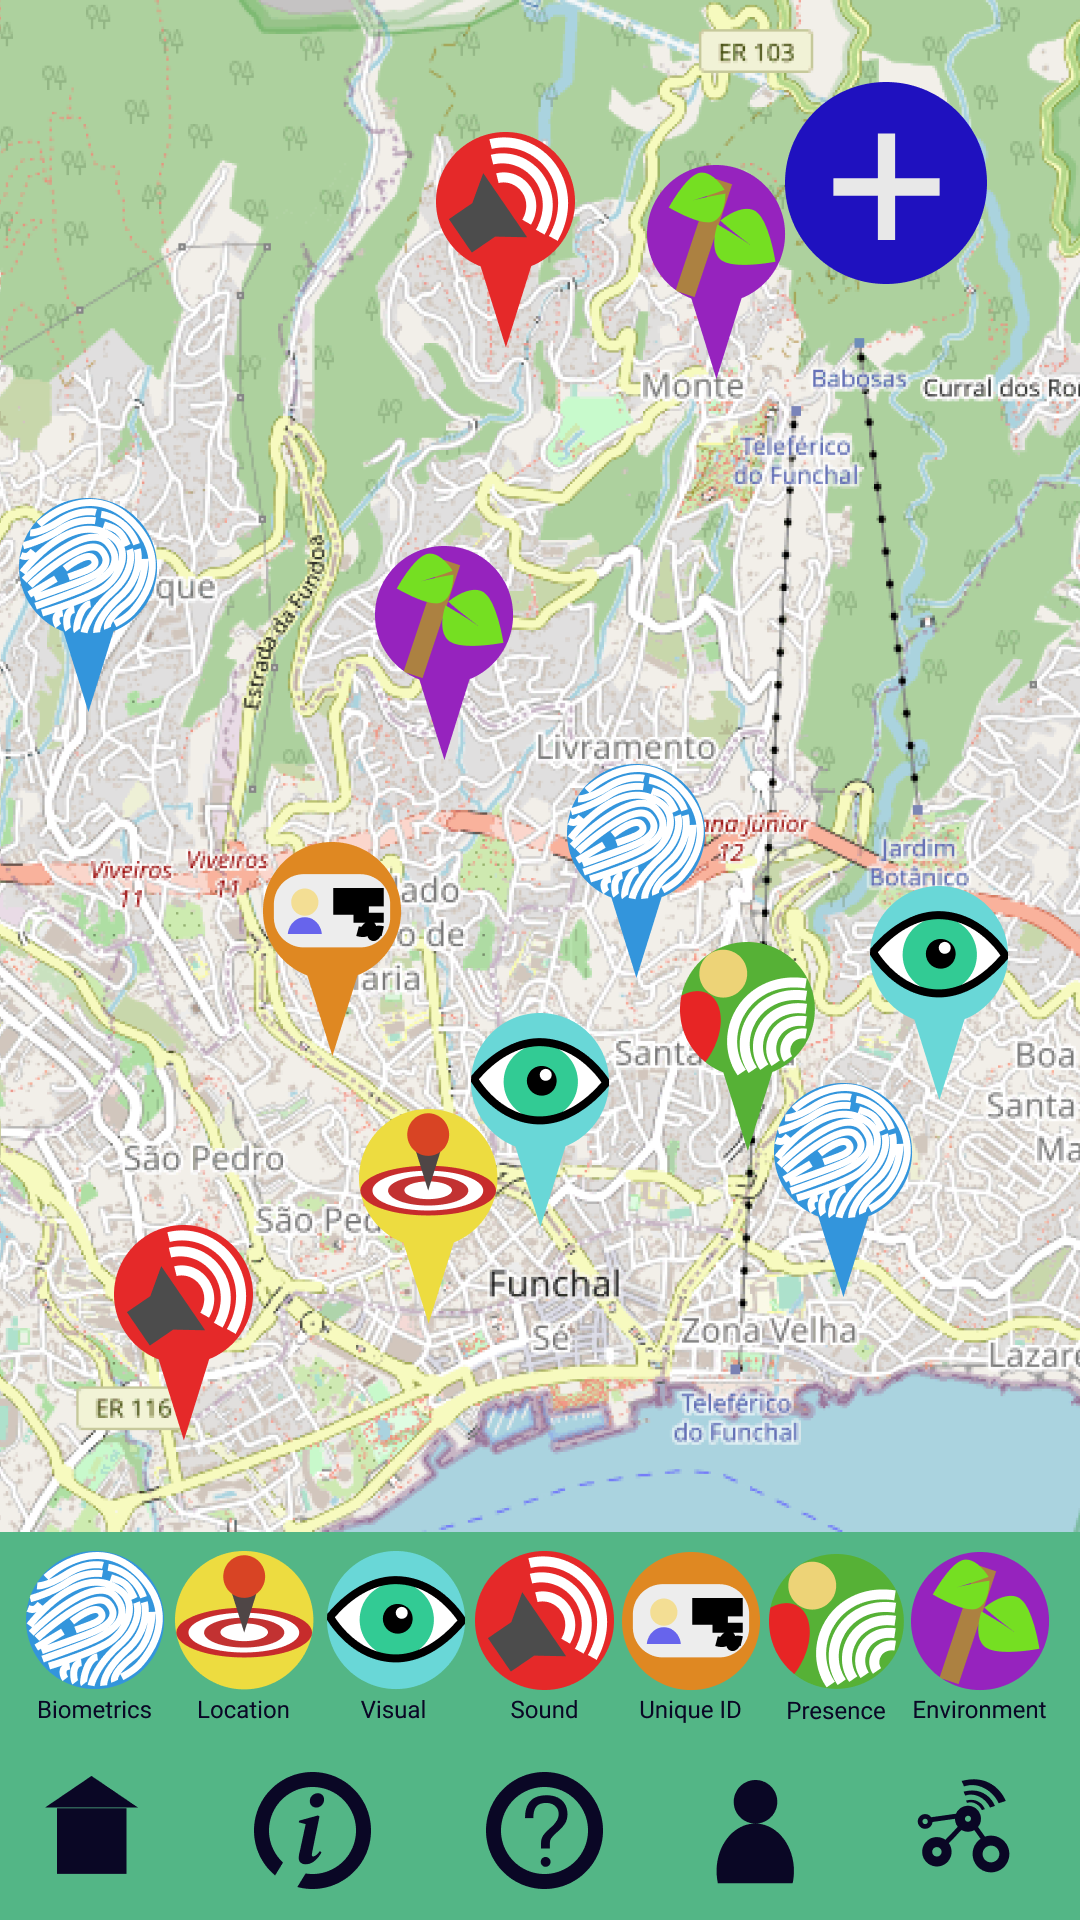
\includegraphics[width=130pt]{../assets/images/high_homepage.png}
        \caption{}
        \label{fig:highhome}
    \end{subfigure}%
    \begin{subfigure}{0.33\textwidth}
        \centering
        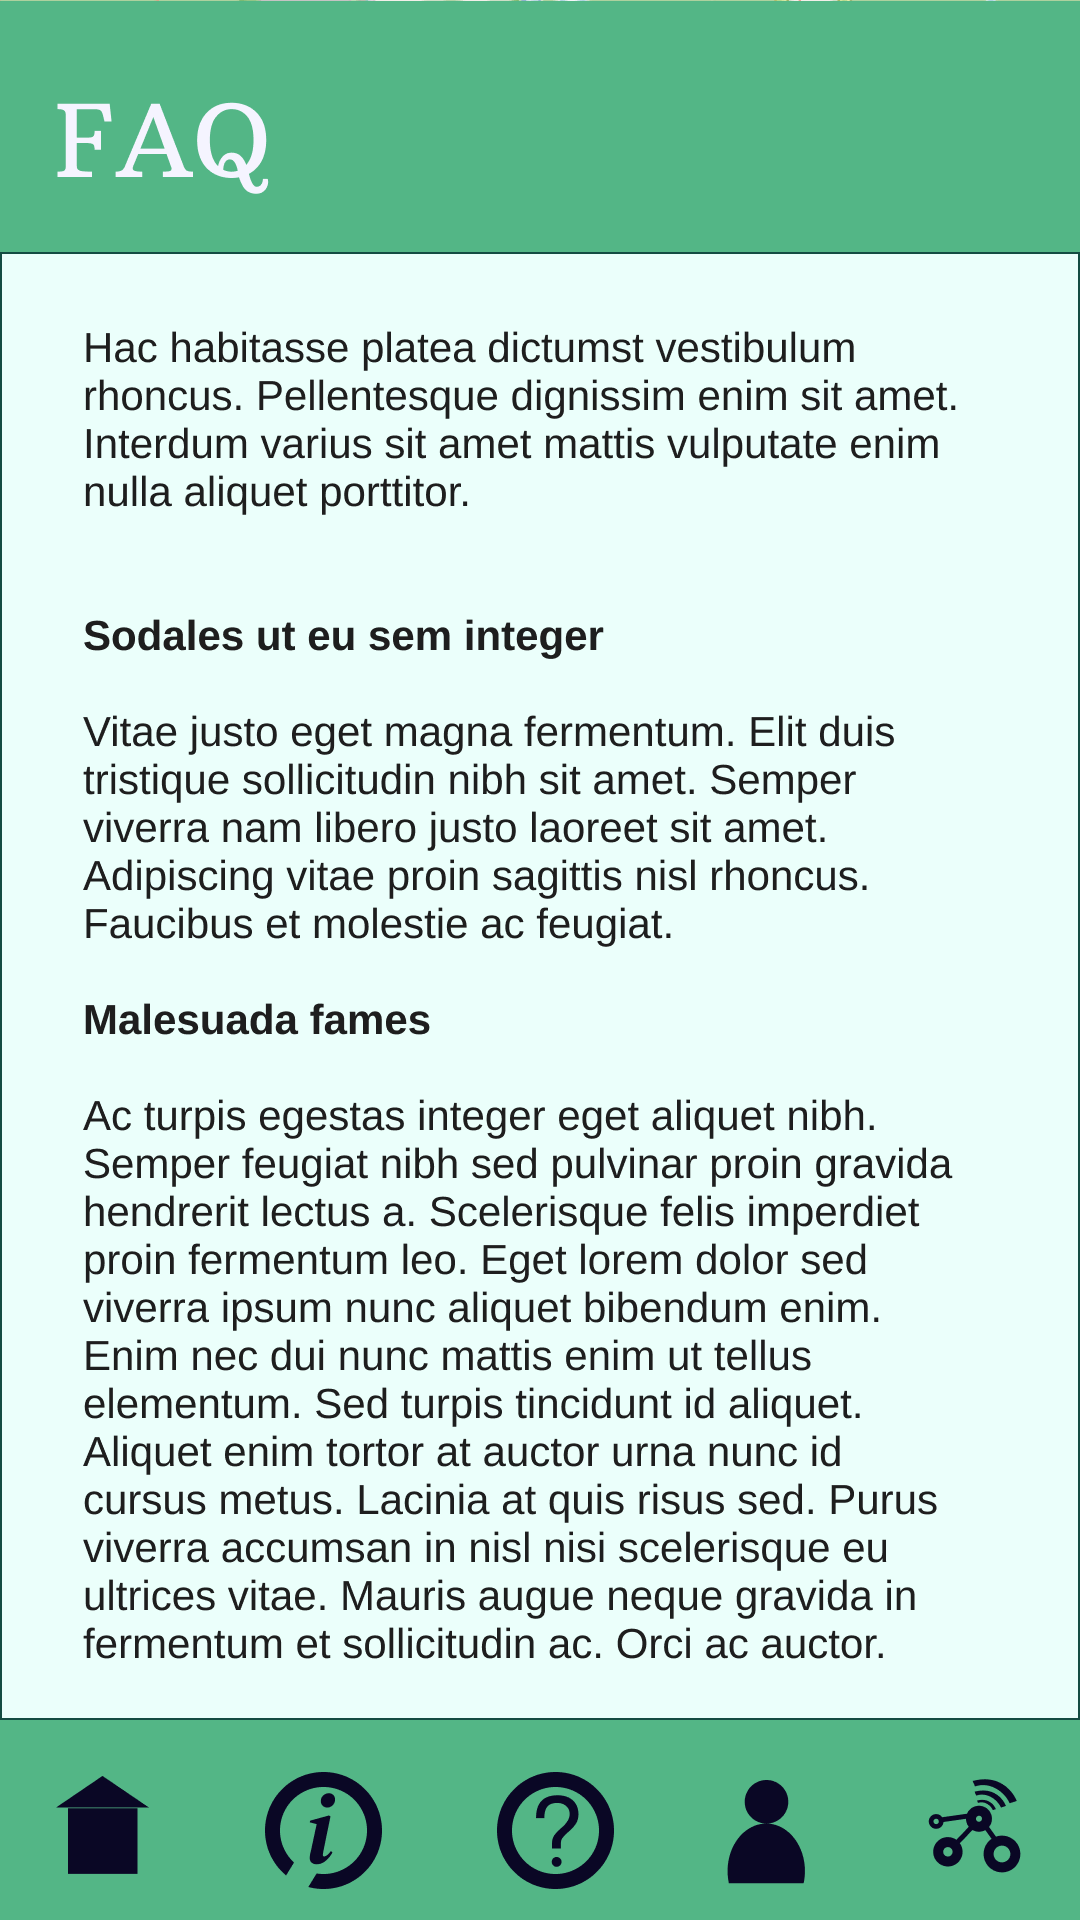
\includegraphics[width=130pt]{../assets/images/high_more_info.png}
        \caption{}
        \label{fig:highabout}
    \end{subfigure}%
    \begin{subfigure}{0.33\textwidth}
        \centering
        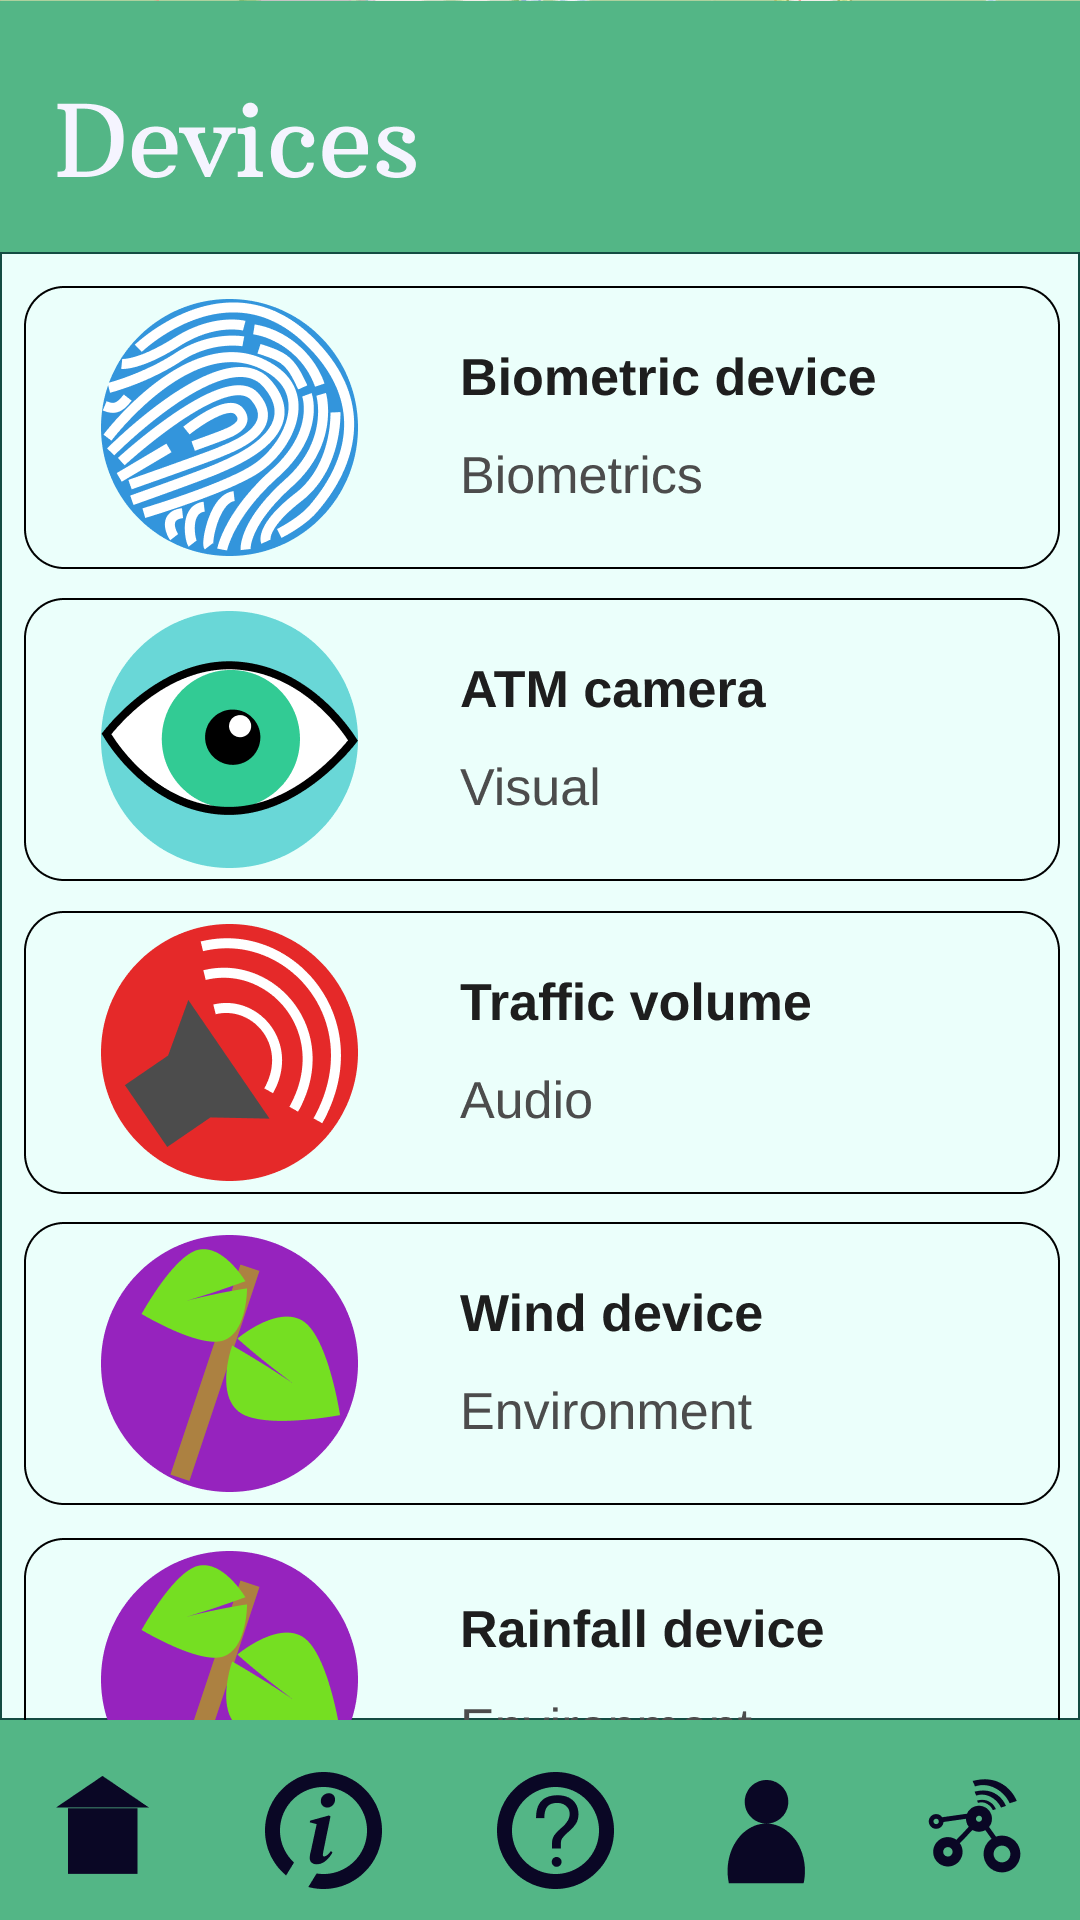
\includegraphics[width=130pt]{../assets/images/high_devices.png}
        \caption{}
        \label{fig:highfaq}
    \end{subfigure}%
    \caption{High level prototype of (a) homepage, (b) about and (c) FAQ pages.}
    \label{fig:highlevelprototype}
\end{figure}

After doing the prototypes, development was started, although some overlap
happened with the high level version prototype, as the icons for the categories
were being created. Figure \ref{fig:live_app} represents the application pages:
(\ref{fig:livehome}) homepage, (\ref{fig:liveabout}) about, (\ref{fig:livefaq}) more
information, (\ref{fig:live_devices}) IoT devices, (\ref{fig:live_device_info}) device
and (\ref{fig:live_statistics}) statistics.
Further changes would occur between the prototypes and
the application, such as the colour scheme, icons for pages that were created
were not used.

\begin{figure}[H]
    \centering
    \begin{subfigure}{0.30\textwidth}
        \centering
        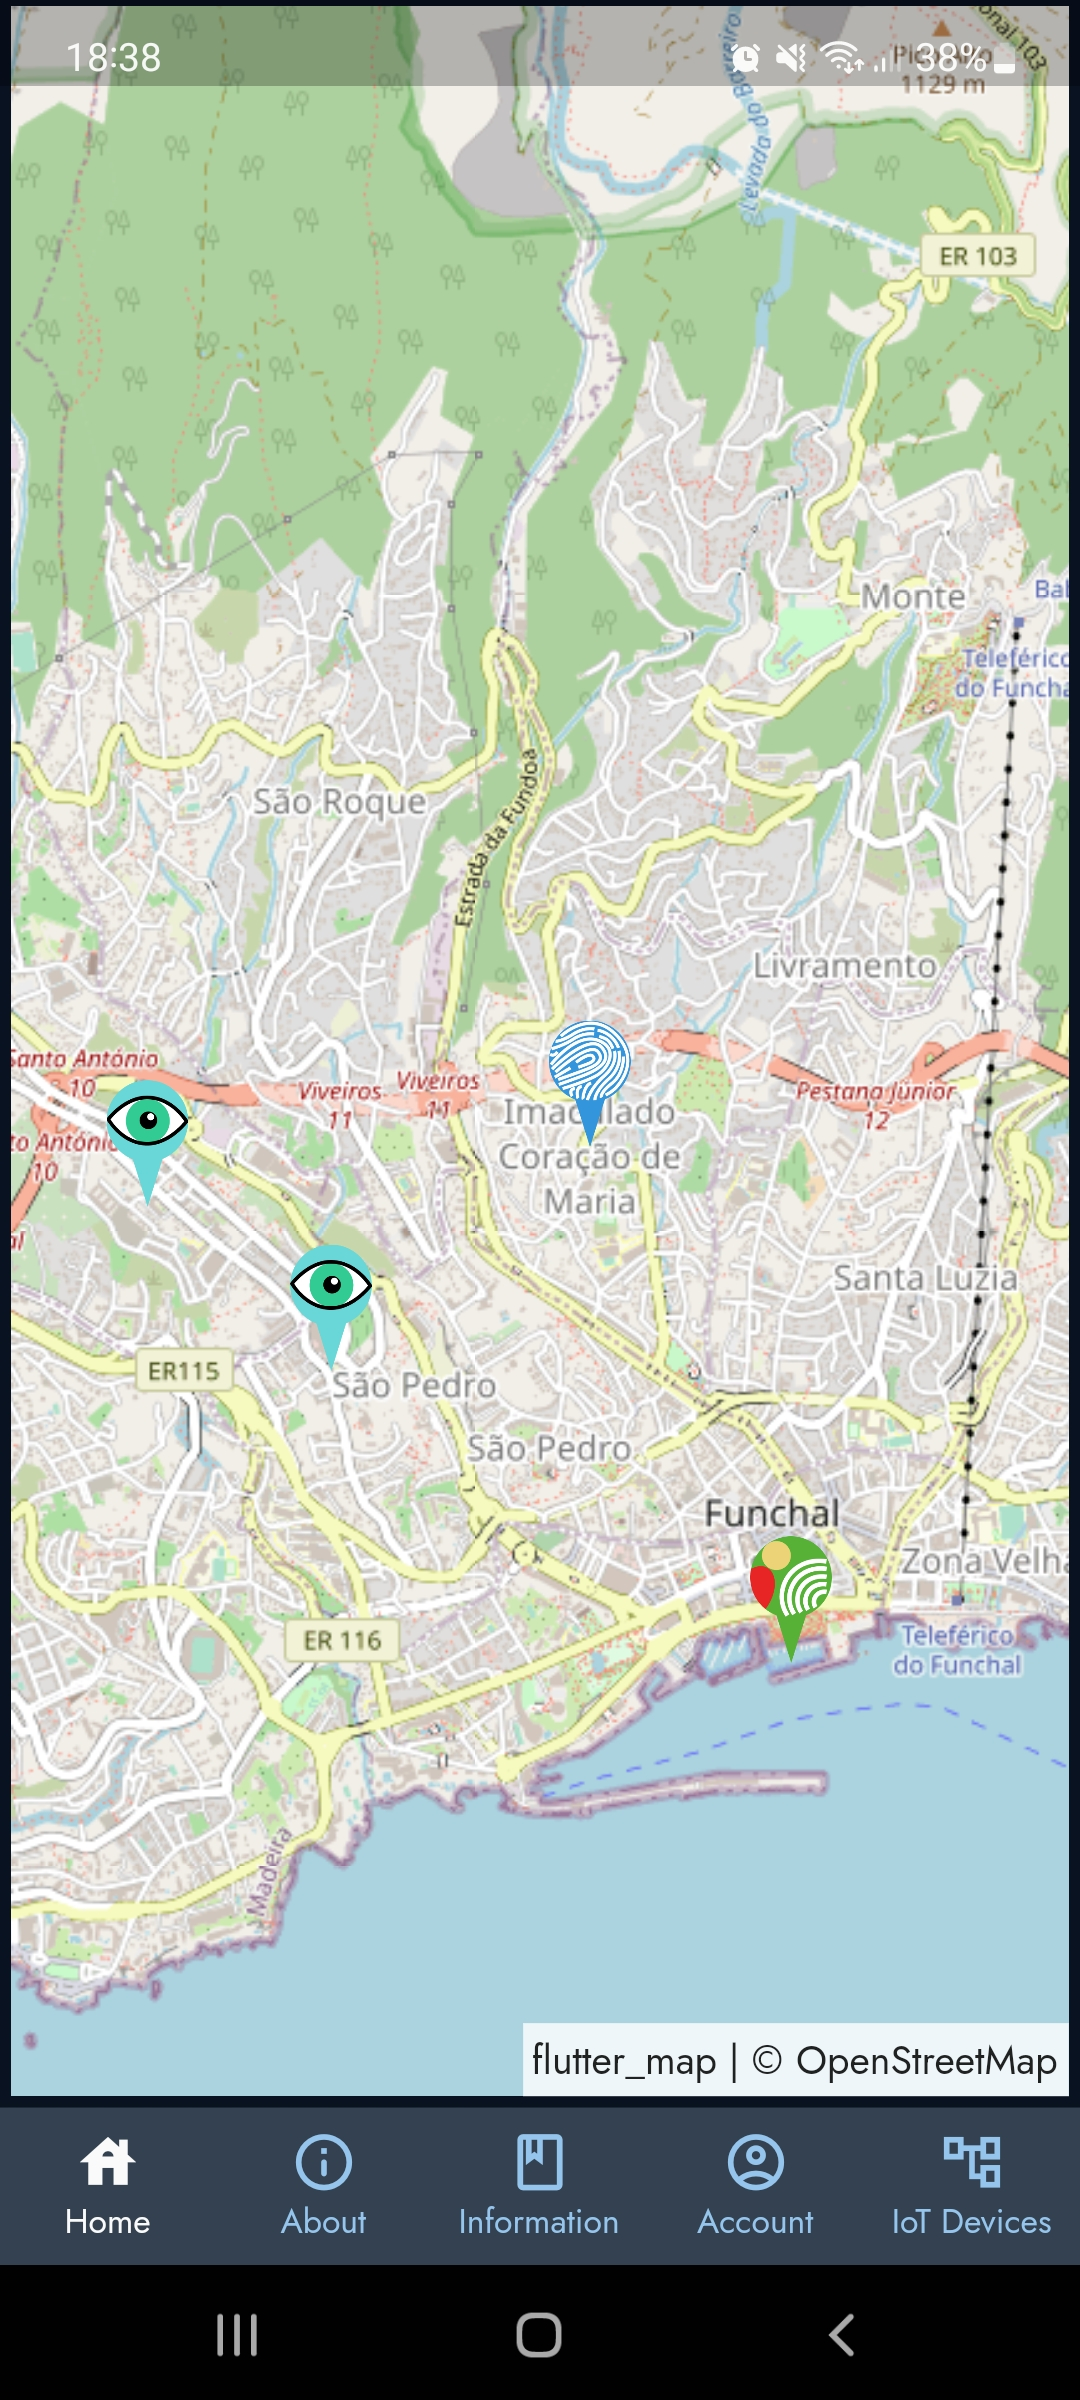
\includegraphics[width=125pt]{../assets/images/live_homepage.jpg}
        \caption{}
        \label{fig:livehome}
    \end{subfigure}
    \begin{subfigure}{0.30\textwidth}
        \centering
        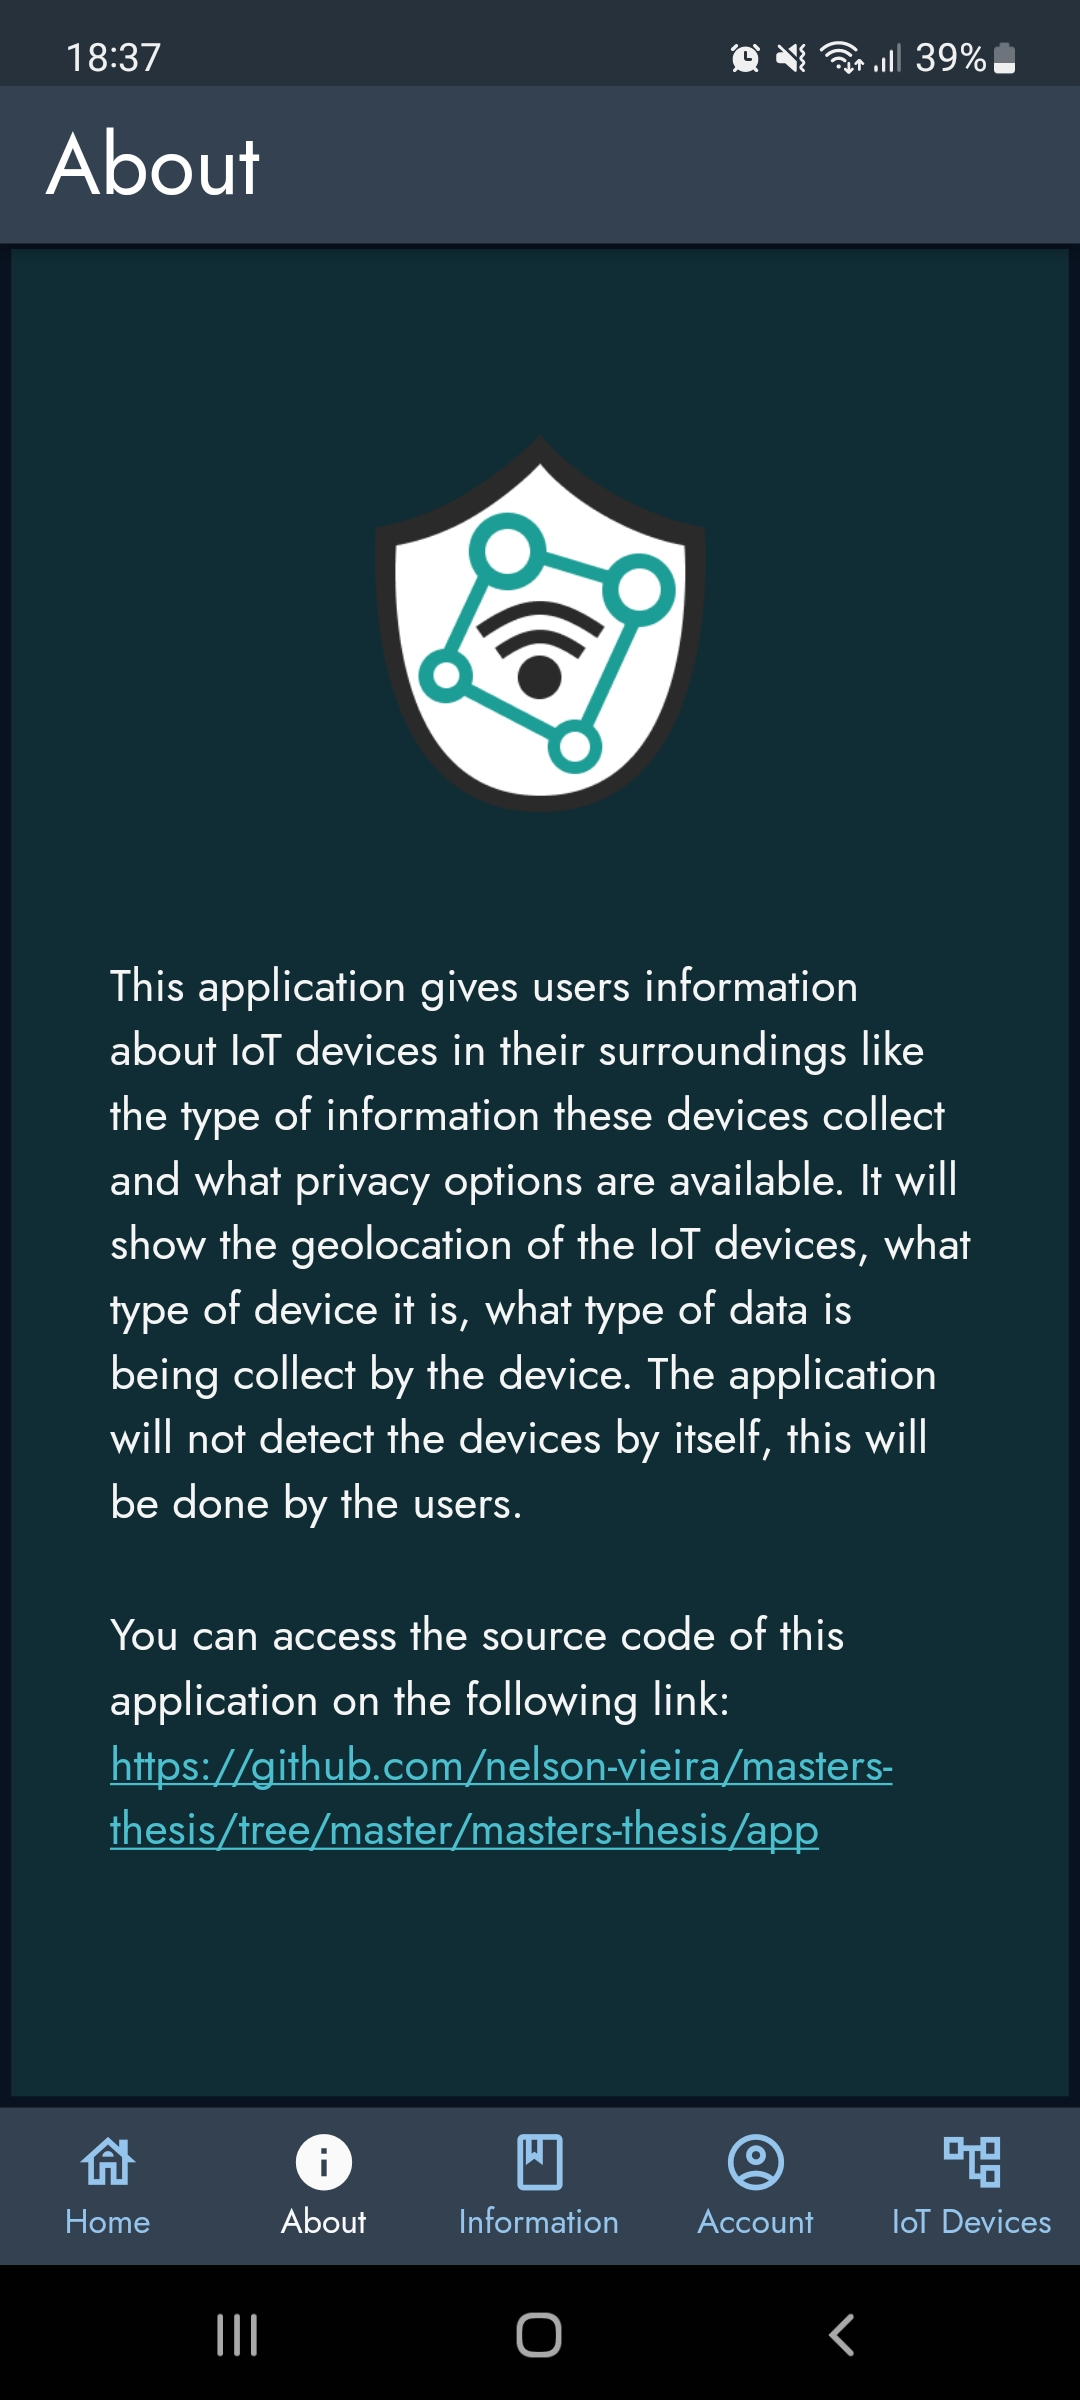
\includegraphics[width=125pt]{../assets/images/live_about.jpg}
        \caption{}
        \label{fig:liveabout}
    \end{subfigure}
    \begin{subfigure}{0.30\textwidth}
        \centering
        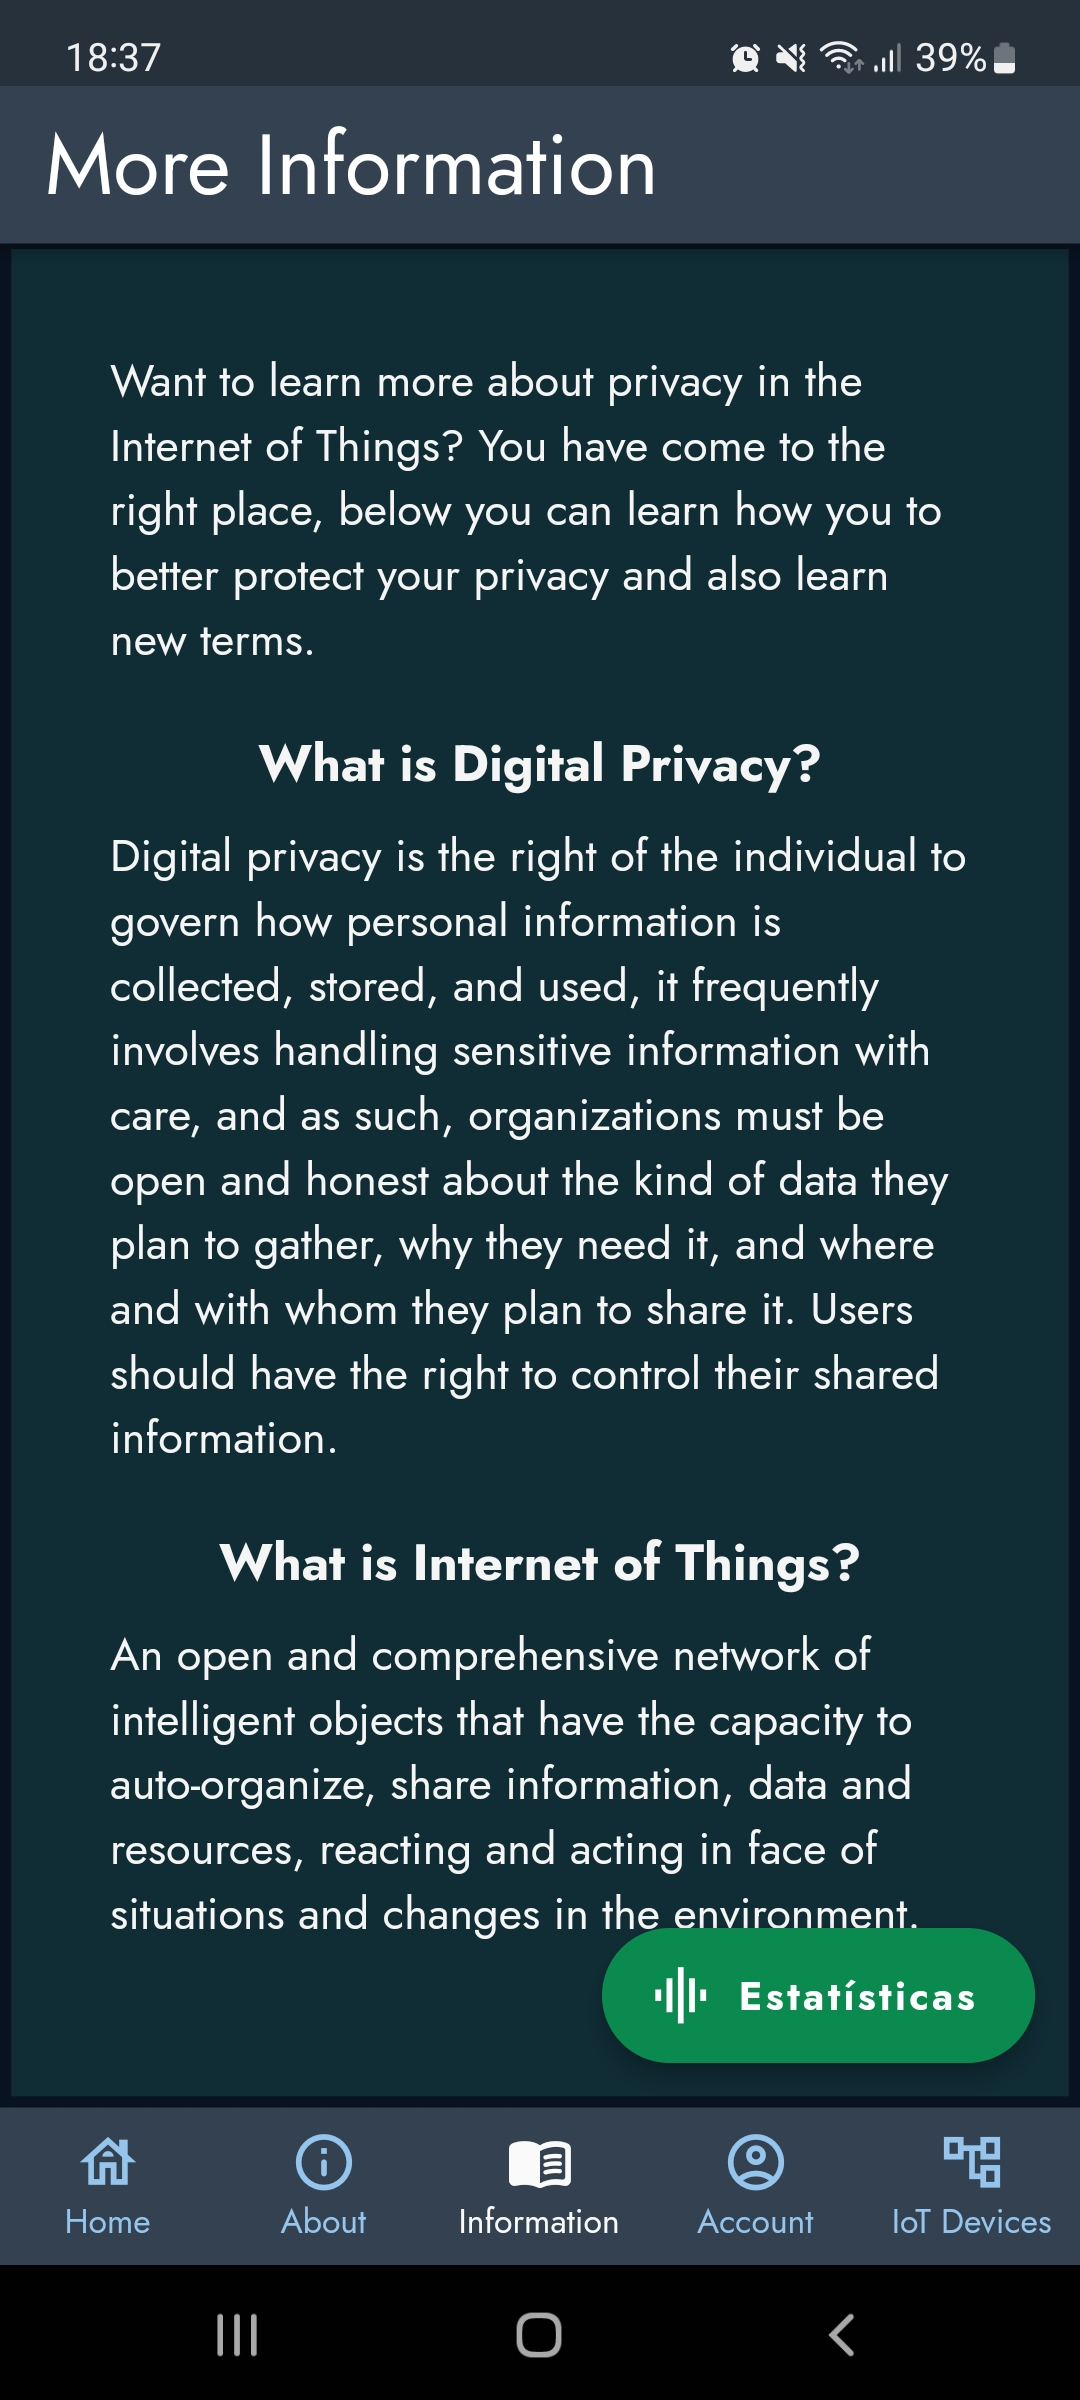
\includegraphics[width=125pt]{../assets/images/live_more_info.jpg}
        \caption{}
        \label{fig:livefaq}
    \end{subfigure}
    \begin{subfigure}{0.30\textwidth}
        \centering
        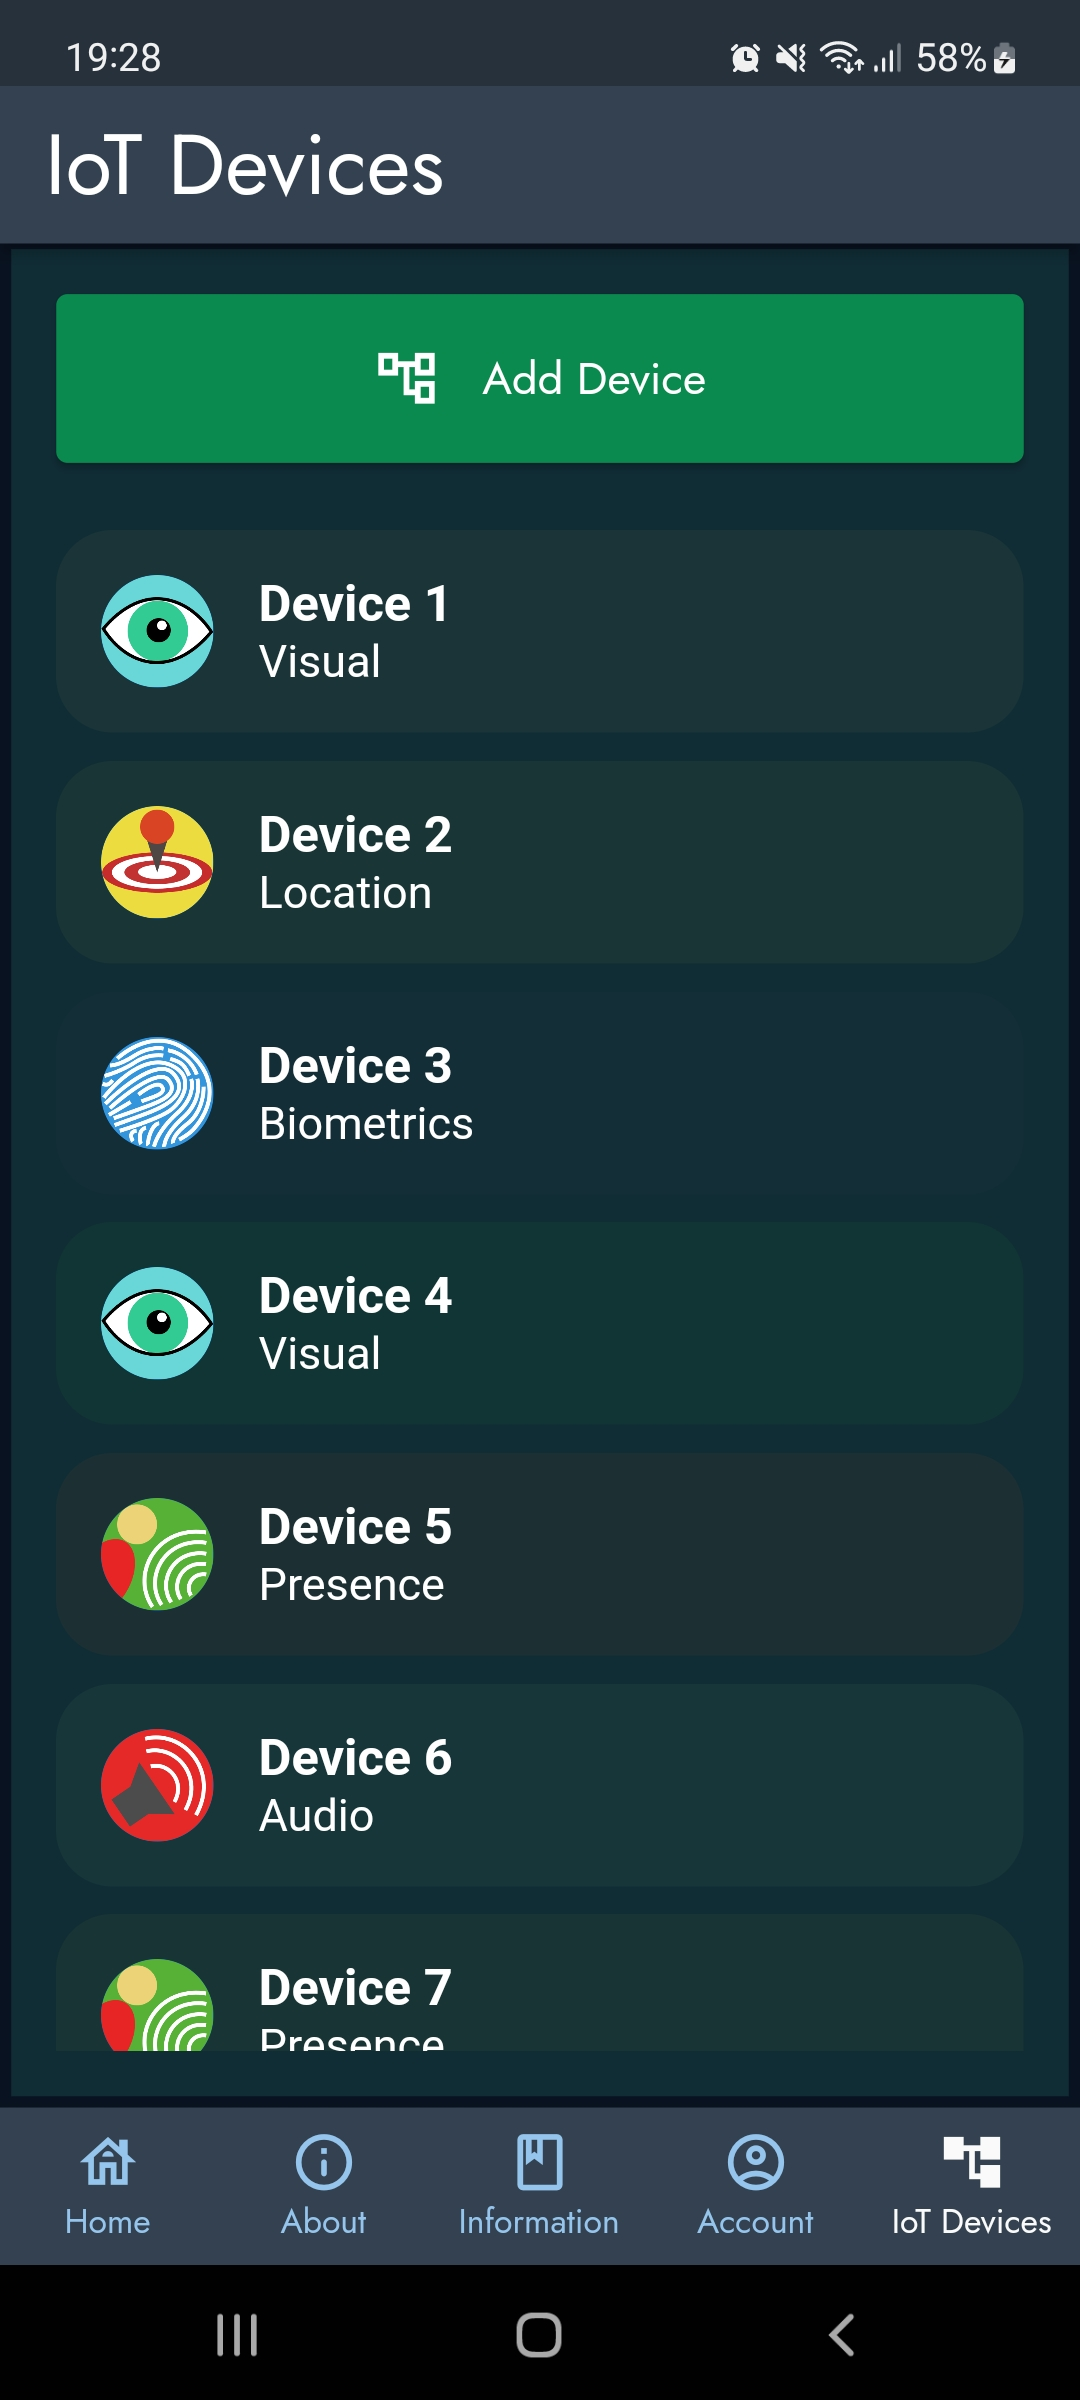
\includegraphics[width=125pt]{../assets/images/live_devices.jpg}
        \caption{}
        \label{fig:live_devices}
    \end{subfigure}
    \begin{subfigure}{0.30\textwidth}
        \centering
        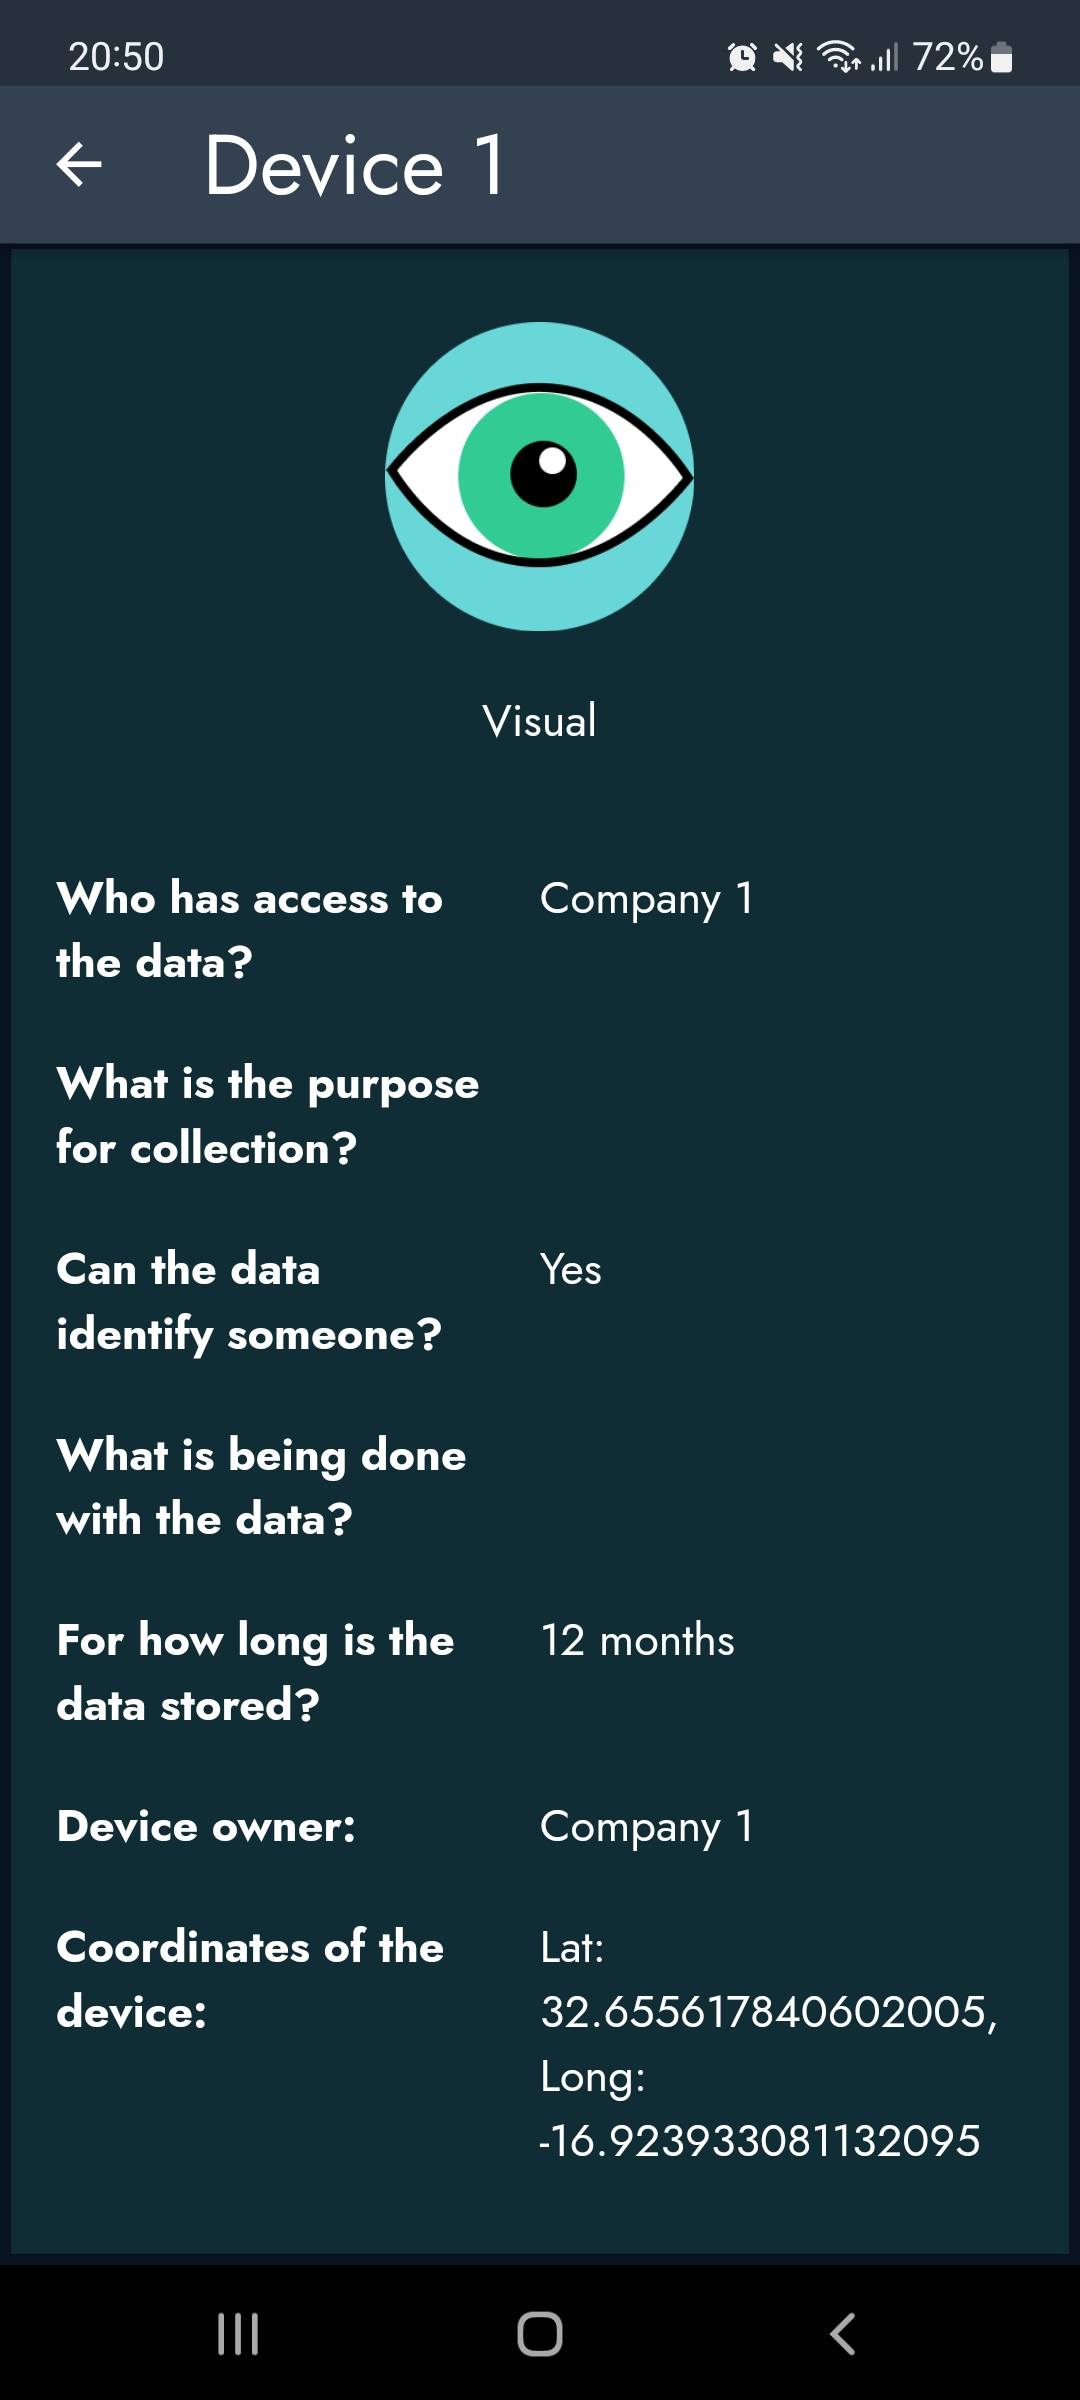
\includegraphics[width=125pt]{../assets/images/live_device_info.jpg}
        \caption{}
        \label{fig:live_device_info}
    \end{subfigure}
    \begin{subfigure}{0.30\textwidth}
        \centering
        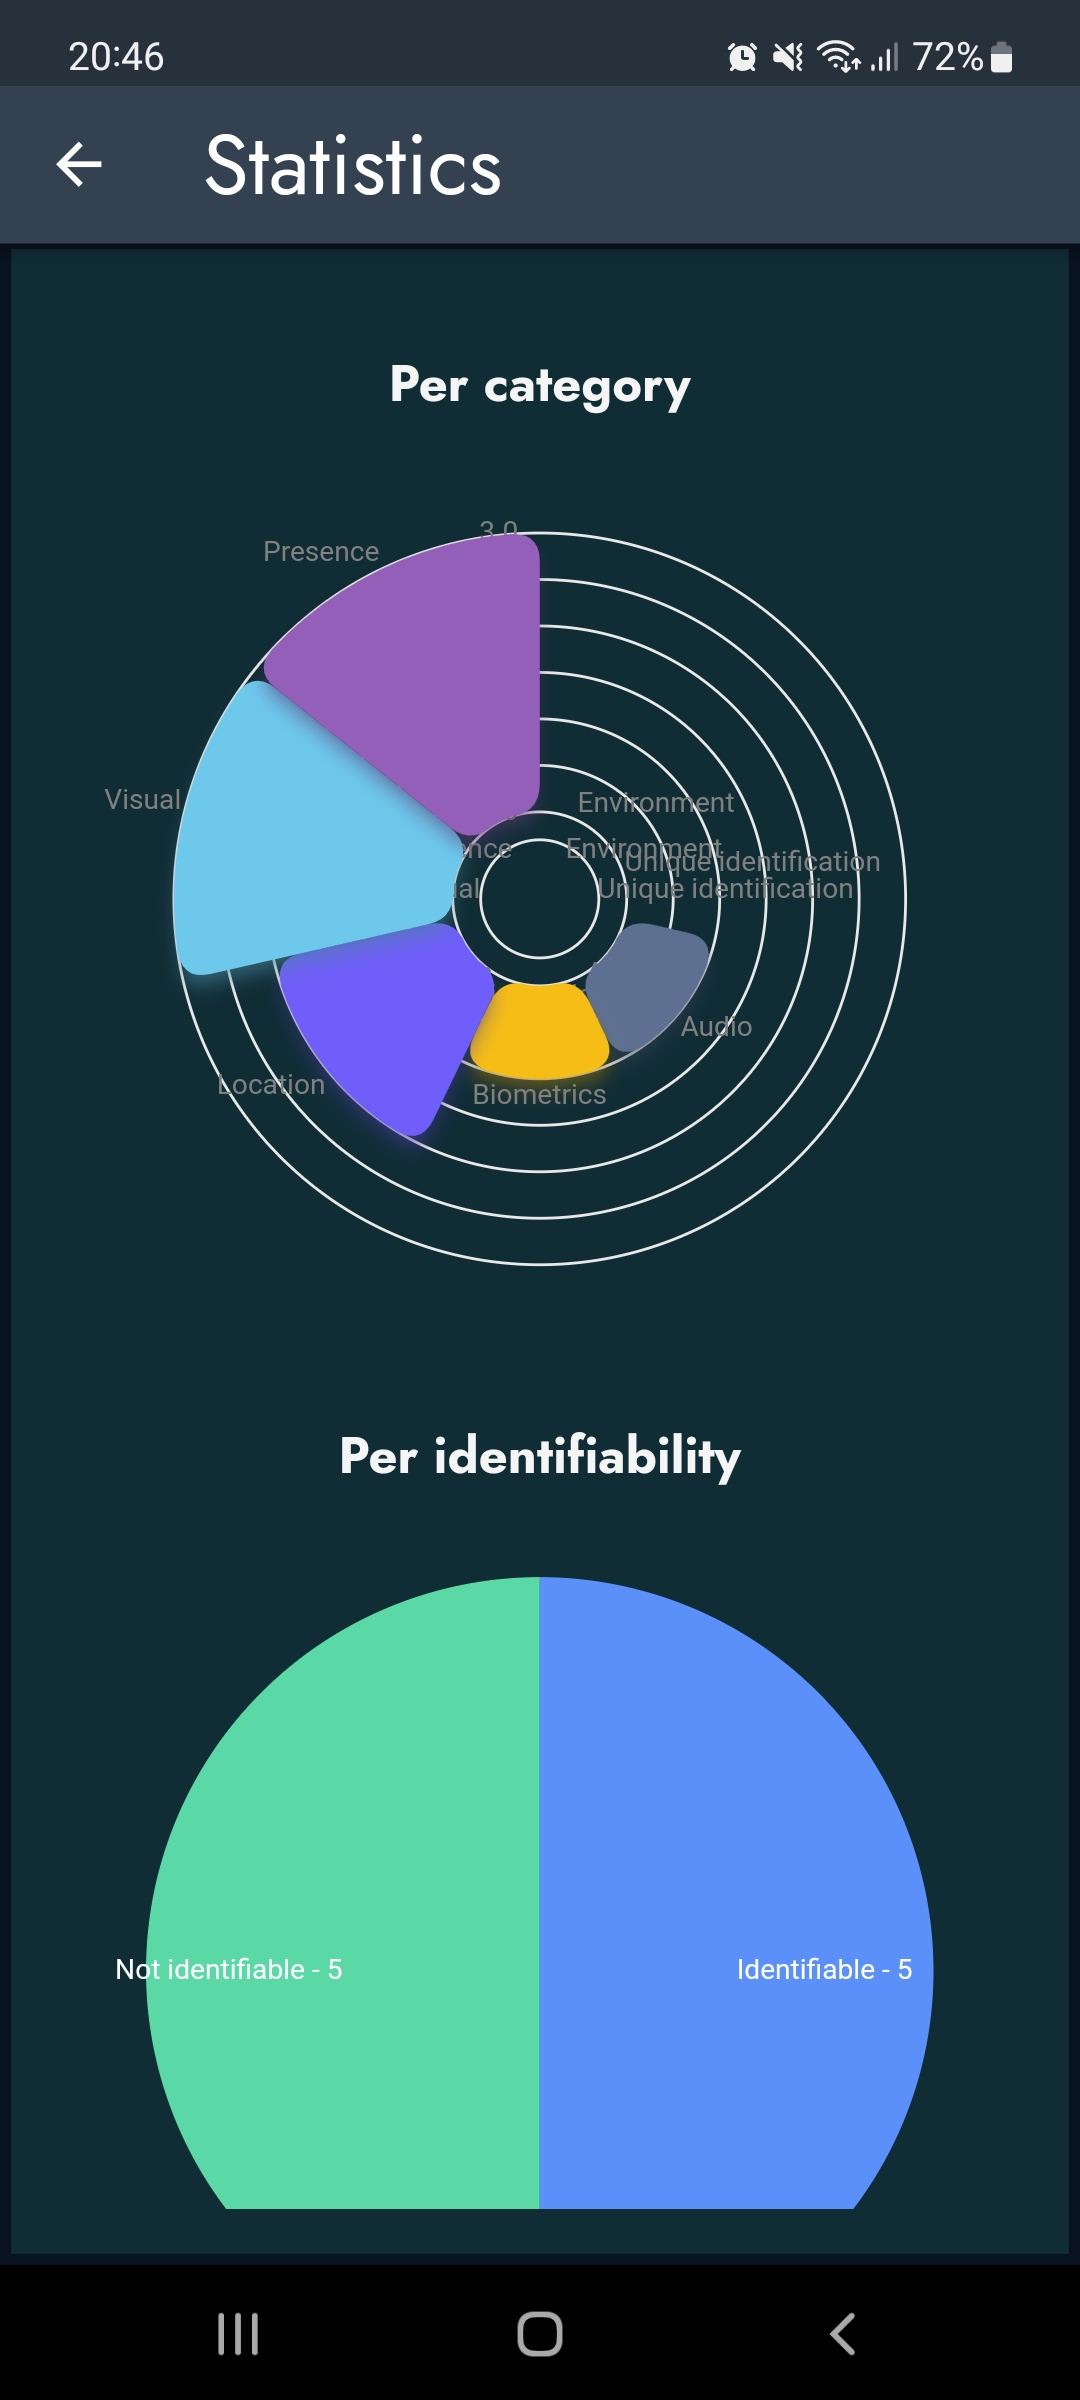
\includegraphics[width=125pt]{../assets/images/live_statistics.jpg}
        \caption{}
        \label{fig:live_statistics}
    \end{subfigure}
    \caption{Live version of the application with pages: (a) homepage, (b) about, (c) FAQ, (d) devices, (e) device information and (f) statistics pages.}
    \label{fig:live_app}
\end{figure}

\subsection{Development}

As was defined in the system requirements specification, the Flutter
framework was the development tool used for the reasons described.
This allows for the relatively fast development of an application for
mobile without using native tools, which would significantly lengthen the
development time.

Figure \ref{fig:dbmodel} shows an entity relationship diagram, this type of
diagram is usually created for relational databases, but, as is the case of
Firestore, the database used is document-oriented, or NoSQL. This differs from
relational databases in that data is stored in an object rather than in separate
tables with relationships between them, but it can work identically to a relational
database if configured properly. One of the main reasons to use Firestore is that
it has great integration with Flutter. There are only three documents used to
store backend data, one for IoT devices, one for users and another for categories.
A document for users is used to extend Firebase Authentication, which can only
store the email and password of users and also be used for email confirmation.

\begin{figure}[H]
    \centering
    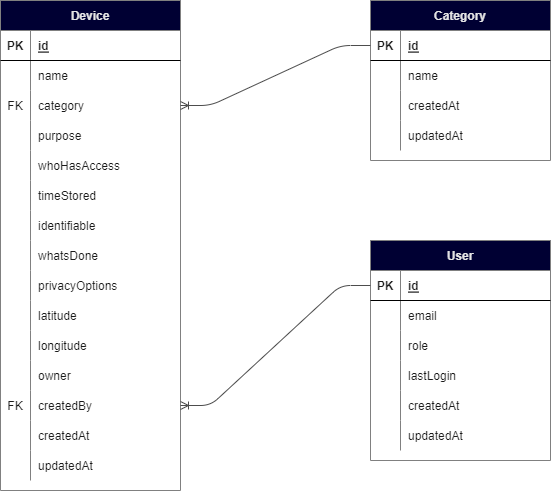
\includegraphics[width=340pt]{../assets/images/erdiagram.png}
    \caption{Entity relationship diagram of database.}
    \label{fig:dbmodel}
\end{figure}

The development phase of this work took the greatest amount of time,
it started almost after carrying out the requirements assessment, while
the prototypes were being created and continued after conducting the
usability tests. It will still be continued to be developed even after
the production version 1.0 is released.

What makes it take so much time is due to the resolution of bugs and
problems that appear during the normal course of development. Using
the Firestore database proved to be somewhat difficult because
it is not as intuitive to create queries between different objects
as it is using the SQL language.

Users can, when they start the application for the first time, freely use it to see
which devices are in their vicinity,
information about the devices, information about the application itself, and
information about privacy in general and more specifically privacy in IoT systems
which they can use to improve their digital literacy. What they cannot do is
add a new device to the application or edit a device's information. The user has
to create an account first to do these operations. The decision to add an
account creation before the user can add or edit a device is to prevent
bad actors to add bogus data to the application making unusable for the majority
of people, this solution doesn't completely solve this issue (because bad actors
can still create an account and add bogus data anyway) but it helps to slow
down the insertion of bad data.

Upon account creation the only data entry that can be considered sensitive that
the user has to input is an email address.
After the user has created an account and logs in, the user can add devices to the application with the following information:

\begin{itemize}
    \item[$\bullet$]
    The \textbf{name of the device}: This serves to differentiate between the various devices on the application and as such should be unique to each device, it is used on various routes and is one of the first fields that users see about a device. A single device does not have an \textit{official} name, what is more probable is that the device has a model name or is part of a system with it's own name. The user creates the name, this could be abused by bad actors but it is extremely discouraged. It is used for aesthetic reasons.
    \item[$\bullet$]
    The \textbf{category of the device}: This is used to categorize each devices main type of information that the device is collecting. These can be of the following:
    \begin{itemize}
        \item[$\circ$] \textbf{Visual}: The device mainly collects visual information with maybe a video camera.
        \item[$\circ$] \textbf{Audio}: The device mainly collects audio information with a sound recorder.
        \item[$\circ$] \textbf{Presence}: The device can detect the presence of nearby objects or persons. This is not the same as the location category because the device does not know the location of an individual, it merely knows that the individual is nearby. These type of devices can be used, for example, to collect information about how many people frequent a specific store.
        \item[$\circ$] \textbf{Location}: The device can detect the exact or approximate location of an individual, it can use GPS to get this kind of information.
        \item[$\circ$] \textbf{Biometrics}: The devices collects biometric data, this can be the number of steps an individual (or animal) takes, or health related data like the heart beat.
        \item[$\circ$] \textbf{Environment}: These type of devices collect environmental data, they can be used for agriculture or weather forecasting by collecting, for example, temperature, humidity or wind speed/direction data.
        \item[$\circ$] \textbf{Unique identification}: This category is for a device that can uniquely identify an individual, the device itself most likely is not capable of doing it but with other information that the device has access to, it can be used to cross reference of information and as such uniquely identify a person. An example of this would be a device a device that can collect visual data and with facial recognition used against other data in a database it can uniquely identify an individual.
    \end{itemize}
    \item[$\bullet$]
    The \textbf{purpose for the data collection}: Defines what is the purpose for the collection of the data, if a device collects temperature and humidity data and is used by a weather based company or government agency then the purpose for the data collection is for weather forecasting.
    \item[$\bullet$]
    \textbf{Who has access to the collected data}: Disclose an individual or group of individuals that have access to the data of the device, if the device is part of a closed system it can be that only an individual as access to the data but most likely various groups of people have access to the data, some with more data than others depending on the permissions they have. If the device publicizes its data then everyone has access to it.
    \item[$\bullet$]
    \textbf{For how long is the data stored}: Pinpoint the duration of the stored data in the device or system, due to legislation passed in various countries this duration has a limit, in some cases the data cannot be stored for more than one year.
    \item[$\bullet$]
    \textbf{Can the data identify anyone}: Used to quickly identify if a particular device can identify an individual or not. If the device belongs to the ``Unique identification'' category then this should be active.
    \item[$\bullet$]
    \textbf{What is being done with the data}: This could be assumed to be similar to the \textbf{purpose} field mentioned above but it should be used to diagnose what is being done now with the data collected, in certain situations it might coincide with the purpose for the data collection.
    \item[$\bullet$]
    \textbf{Privacy options}: The user can insert an url for the device's privacy options, in some cases the device, or company, has a website with information on privacy options, or privacy policy. If the device uses a mobile application then a link to the this application can be inserted here.
    \item[$\bullet$]
    \textbf{Coordinates of the device}: Used to express the latitude and longitude of the device so that it can be shown on the map, on the homepage of the application.
    \item[$\bullet$]
    \textbf{Who owns the device}: Who is the device owner, if it belongs to an organization then the name of the organization should appear here otherwise if the device belongs to a person then the person's name should \textbf{not} appear, it should say private or something similar.
\end{itemize}

The user is not required to provide information to satisfy all items on this list, the
only information that is required in order to add a device to the application is
the name, category and coordinates of the device, all other
information is optional but should be provided for the sake of guaranteeing a good
experience to other users of the application. The information provided
should be verified by the user beforehand so that bogus data does not clutter
the application, in this case there are no absolute ways of guaranteeing this
but the maintainer of the application edit wrong information or in some
cases remove it, other users can also edit any device data. This is an
open platform so it is expected that users act in good faith.

The usability tests were crucial to the development of the application,
they improved significantly the user experience along with changes to the
user interface.

Usability tests were conducted in person with 7 participants of different
ages, professional fields and qualifications. The participants ages fall
under the 40-50 range, the professional fields include accounting,
management, social services and agriculture, and qualifications range from
basic education to bachelor's degree. Unlike the dissemination of the questionnaire,
participants for these tests were recruited informally. Before doing the tests,
some questions were made to evaluate the general level of digital literacy
regarding IoT and privacy, then the participants were asked to fill in the
survey, if they had not done it yet, as this gives some insight into what the
application is about. The usability tests consisted of single ease
questions \cite{tedesco2006comparison}
and the system usability scale \cite{brooke1996sus}, as can be seen on \nameref{appendix:usability_tests}.
The single ease questions were used after the participant performed each task, the
participant would answer how difficult they though the task was in a
scale from 1 to 7. The system usability scale was used after the participants
performed all tasks, with the same type of scale.

    \clearpage
    % SPDX-License-Identifier: CC-BY-4.0
%
% Copyright (c) 2023 Nelson Vieira
%
% @author Nelson Vieira <nelson0.vieira@gmail.com>
% @license CC-BY-4.0 <https://creativecommons.org/licenses/by/4.0/legalcode.txt>
\section{Methodology}

The overall work will be comprised of two phases which will be described
in the following paragraphs. Phase one mainly described throughout this
paper, focuses on collecting the state of the art in terms of the most relevant
topics, from which main privacy concepts were selected to be explored in
the stage 1 of Phase 2 with the preparation of a questionnaire to collect
user perceptions regarding privacy and topics collected in the systematic
literature review. The second stage of Phase 2 consists in developing an
application, partially based on the information generated by the survey,
that can identify what sort of devices are around, what kind of data is
gathered by these devices, present privacy options to the user when available,
and what can be done to prevent undesirable data from being collected.
\par
The Phase 1 Systematic Literature Review gathered the most relevant papers
discussing methodologies and techniques for the protection of users' privacy
data with special focus on IoT systems. For this SLR, this paper considered
focusing only on papers from the last 12 years, from 2010 until 2022, since
papers before then become out of date with the evolution of technology.
In this SLR, it was reviewed 54 papers published in top computer science,
security, privacy and software engineering outlets.

This paper followed Keshav's three-pass approach \cite{KeshavHow} when choosing
which papers to read fully and which ones to ignore, first the title would
be read, then the abstract, the introduction and conclusion and briefly
skim the rest of the paper and then decide if it was worth reading any further,
the focal point in this phase was answering the following question: does
the paper present a new methodology or interesting angle to tackle users'
privacy concerns? Only then the document would be read in its entirety while
ignoring any tables, figures, images or graphs. If the paper failed to present
any interesting idea, approach, or technique it would be discarded, but
if not, it would be read carefully from the beginning again in order to
fully understand what it presents. Having collected the major findings,
this work then aims to conduct a throughout study split in several stages
and around the specific research questions which will be explored in each
phase. For that matter, the research questions listed are:

\vspace{5mm}
\textbf{Phase 1:} \\
% \vfill

\textbf{RQ1:} What approaches are being considered for privacy issues in
IoT in the currently available literature?

\textbf{RQ2:} What are user perceptions on online privacy? \\

% \vspace{5mm}
\textbf{Phase 2:} \\
% \vfill

\textbf{RQ3:}
% What IoT-related tools are available that empower users to
% protect their privacy rights? OR
How to empower users to protect their privacy rights?

\textbf{RQ4:} What issues are prevalent in IoT that make it difficult to
address privacy and security problems?
\vspace{5mm}

The second phase will be evaluated on two stages, the first one consists
on doing a study on people's general privacy concerns, while using and interacting
with IoT devices. This study will abide on preparing a questionnaire to
assess general user's knowledge on privacy concepts, their habits and concerns,
their understanding of privacy rights, and what they do to safeguard those
rights. The goal of this study is to both understand the privacy paradox
and collect data on their proposal to address privacy issues with regard
to IoT devices.

% Having collected the major findings, this work then aims to conduct a throughout
% study split in several stages and around the following research questions:

% \textbf{RQ1:} What approaches are being considered for privacy issues in
% IoT in the currently available literature?

% \textbf{RQ2:} What IoT-related tools are available that empower users to
% protect their privacy rights? OR How to empower users to protect their privacy
% rights?

% \textbf{RQ3:} What issues are prevalent in IoT that make it difficult to
% address privacy and security problems?

% The proposed methodology is composed of two phases, the first phase consists
% on doing a study on people's general privacy concerns while using and interacting
% with IoT devices. This study will consist on preparing a questionnaire to
% assess general user's knowledge on privacy concepts, their habits and concerns,
% their understanding of privacy rights, and what they do to safeguard those
% rights. The goal of this study is to both understand the privacy paradox
% and collect data on their proposal to address privacy issues with regard
% to IoT devices. The second phase consists in developing an application, partially
% based on the information generated by the survey, that can identify what sort
% of devices are around, what kind of data is gathered by these devices, present
% privacy options to the user where available, and what can be done to prevent
% undesirable data from being collected.

% The second phase consists
% in doing an application that can detect IoT devices nearby the user with
% at least a 10 meters radius. The application should do the following when
% detecting a device:
% 1. it should show some information about the device;
% 2. it should categorize the device;
% 3. it should provide the user with privacy options, if the device allows the
% user to decline data harvesting.
% This application at first sight might appear to be a mere privacy assistant
% but it's not, because IoT assistants merely choose what privacy options the
% user first sets and maintains it for every other application that the user
% might use. The proposed app doesn't have the objective to conform to the user's
% preferred privacy choices, it merely informs the user about nearby IoT devices
% and can provide the user with privacy options. But the main objective is creating
% awareness in individuals about the various devices that are around and make
% the user questions their choices.

\subsection{Stage 1: User perceptions}

This study aims to understand people's perception of IoT and their privacy
practices online. It also serves to demystify the privacy paradox and also
to help provide a solution to the privacy issue in IoT. The questionnaire
consists of 92 questions divided into 7 sections to access users' knowledge,
it follows a kind of narrative, the first section being general privacy
questions then about the predisposition to data sharing, to concerns with
privacy then about daily digital routines, then about profile identification,
and then about IoT general knowledge before a section about non-identifiable
demographic data. The scale that is used in the questionnaire is based on
the work of Philip K. Masur \cite{masur2018situational}. Great care is taken
when it comes to this survey's data collection, in order to not identify
any individual or group of individuals, for instance, when it comes to differential
privacy, any data that might identify someone will not be disclosed, even
though the data might suffer from some inaccuracy because of this.

This survey was partially based in a study done in the Philippines by the
government in the context of their privacy act of 2012 \cite{Philippine2022Conduct},
this was the second survey done on the country's population. It was also
inspired by Alves's master's thesis \cite{alves2021}, which was about citizen's
perception about privacy in the wake of GDPR.

This survey was done through the internet, it was created in Google Forms,
this way it is guaranteed to reach the most people possible, besides Google
Forms itself, it will be used other online venues for distribution and even
printing.

Foram usados vários serviços de divulgação de questionários online
para angariar participantes, todos os serviços usados foram à base
da boa vontade dos participantes, portanto não houve qualquer incentivo
financeiros para o preenchimento do questionário. A maior parte dos serviços
usados são do tipo software as a service (SaaS) e baseiam-se em créditos
pelo preenchimento de outros questionários disponíveis nas plataformas,
isto torna o processo de adquirir participantes muito tedioso, pois
é necessário preencher muitos questionários para conseguir um número
razoável de participantes (pelo menos 400 a 500 participantes). Fazer a
divulgação do questionário desta forma não acarreta qualquer custo adicional,
mas pode fazer com que os resultados obtidos desta forma possam não
ser os mais honestos possíveis, pois alguns participantes podem estar
a preencher este questionário e forma rápida só para também conseguirem
angariar o número de participantes para os questionários deles próprios,
contudo também não há forma de garantir que caso este questionário fosse
realizado com algum incentivo financeiro que os participantes preenchessem
da forma mais honesta possível. Para além da divulgação pelos vários serviços,
também foram usadas as redes sociais e foi divulgado pessoalmente para família e
amigos. Uma forma possível de divulgação seria pessoalmente, de casa em casa, mas
seria esta seria uma forma muito lenta de conseguir respostas e também as
pessoas poderiam se sentir obrigadas a responder e desta forma não seria
muito ético, para além de as respostas poderem ter sido respondidas de uma
forma pouco honesta.

O questionário esteve disponível para preenchimento até ao dia 30 de Abril de 2023,
e durante o tempo em que esteve aberto foi possível obter respostas de x participantes.


\subsection{Stage 2: Study in Context, an Application}

This work proposes an application that gives users information about IoT
devices that inhabit their surroundings, like the type of information these devices
collect and what privacy options are available. This application is developed
for mobile phones due to the fact that these are the most used devices
and people take them everywhere they go, this is important because the application
uses georeferencing to show the location of the IoT devices. This application
has two main objectives, the first is to inform and educate users in order improve
their digital literacy on this particular field (privacy on IoT systems, and
IoT in general) and the other being to give users a way to make informed decisions
to protect their private data, in a concise and convenient place. Generally
the application will show the geolocation of the IoT devices, what type of
device it is, what type of data is being collect by the device. The application
will not detect the devices by itself, this will be done by the users themselves,
in the first iterations of the application it was discussed that the application
itself would automatically detect the devices by using some kind of sniffer
and would categorize what type of device it was and what type of data it
was collecting but it was discovered that this approach was too complex and
so it was not feasible to do with the constraints of this thesis. The application
is developed with Flutter, other options considered were React Native or a
progressive web application, but Flutter uses ahead of time and just in time
compilation, with Dart as it is programming language, while React Native uses
the Javascript programming language that was never created for mobile programming,
so it uses a bridge to convert Javascript to native components for Android
or iOS. Flutter has better performance and as such it was the chosen framework
for this application.

The first step before creating any prototypes or starting the development was
creating a software requirements specification, as can be read on appendix \ref{appendix:a},
delineating the scope and vision for the application; the involved stakeholders;
containing contextual, data-flow and swimlane diagrams; software requirements, including
business, technology, functional and non-functional requirements; use cases
and requirements prioritisation.

Users can, when they start the application for the first time, freely use it to see
which devices are in their vicinity,
information about the devices, information about the application itself, and
information about privacy in general and more specifically privacy in IoT systems
which they can use to improve their digital literacy. What they cannot do is
add a new device to the application or edit a device's information. The user has
to create an account first to do these operations. The decision to add an
account creation before the user can add or edit a device is to prevent
bad actors to add bogus data to the application making unusable for the majority
of people, this solution doesn't completely solve this issue (because bad actors
can still create an account and add bogus data anyway) but it helps to slow
down the insertion of bad data.

Upon account creation the only data entry that can be considered sensitive that
the user has to input is an email address.
After the user has created an account and logs in, the user can add devices to the application with the following information:

\begin{itemize}
    \item[$\bullet$]
    The \textbf{name of the device}: This serves to differenciate between the various devices on the application and as such should be unique to each device, it is used on various routes and is one of the first fields that users see about a device. A single device doen't have an \textit{official} name, what is more probable is that the device has a model name or is part of a system with it's own name. The user creates the name, this could be abused by bad actors but it is extremelly discouraged. It is used for asthethic reasons.
    \item[$\bullet$]
    The \textbf{category of the device}: This is used to categorize each devices main type of information that the device is collecting. These can be of the following:
    \begin{itemize}
        \item[$\circ$] \textbf{Visual}: The device mainly collects visual information with maybe a video camera.
        \item[$\circ$] \textbf{Audio}: The device mainly collects audio information with a microphone.
        \item[$\circ$] \textbf{Presence}: The device can detect the presence of nearby objects or persons. This is not the same as the location category because the device does not know the location of an individual, it merely knows that the individual is nearby. These type of devices can be used, for example, to collect information about how many people frequent a specific store.
        \item[$\circ$] \textbf{Location}: The device can detect the exact or approximate location of an individual, it can use GPS to get this kind of information.
        \item[$\circ$] \textbf{Biometrics}: The devices collects biometric data, this can be the number of steps an individual (or animal) takes, or health related data like the heart beat.
        \item[$\circ$] \textbf{Environment}: These type of devices collect environmental data, they can be used for aggriculture or weather forecasting by collecting, for example, temperature, humidity or wind speed/direction data.
        \item[$\circ$] \textbf{Unique identification}: This category is for a device that can uniquely identify an individual, the device itself most likely is not capable of doing it but with other information that the device has access to, it can be used to cross reference of information and as such uniquely identify a person. An example of this would be a device a device that can collect visual data and with facial recognition used against other data in a database it can uniquely identify an individual.
    \end{itemize}
    \item[$\bullet$]
    The \textbf{purpose for the data collection}: Defines what is the purpose for the collection of the data, if a device collects temperature and humidity data and is used by a weather based company or government agency then the purpose for the data collection is for weather forecasting.
    \item[$\bullet$]
    \textbf{Who has access to the collected data}: Disclose an individual or group of individuals that have access to the data of the device, if the device is part of a closed system it can be that only an individual as access to the data but most likely various groups of people have access to the data, some with more data than others depending on the permissions they have. If the device publicizes its data then everyone has access to it.
    \item[$\bullet$]
    \textbf{For how long is the data stored}: Pinpoint the duration of the stored data in the device or system, due to legislation passed in various countries this duration has a limit, in some cases the data cannot be stored for more than one year.
    \item[$\bullet$]
    \textbf{Can the data identify anyone}: Used to quickly identify if a partitular device can identify an idividual or not. If the device belongs to the "Unique identification" category then this should be active.
    \item[$\bullet$]
    \textbf{What is being done with the data}: This could be assumed to be similar to the \textbf{purpose} field mentioned above but it should be used to diagnose what is being done now with the data collected, in certain situations it might coincide with the purpose for the data collection.
    \item[$\bullet$]
    \textbf{Privacy options}: The user can insert an url for the device's privacy options, in some cases the device, or company, has a website with information on privacy options, or privacy policy. If the device uses a mobile application then a link to the this application can be inserted here.
    \item[$\bullet$]
    \textbf{Coordinates of the device}: Used to express the lagitude and longitude of the device so that it can be shown on the map, on the homepage of the application.
    \item[$\bullet$]
    \textbf{Who owns the device}: Who is the device owner, if it belongs to an organization then the name of the organization should appear here otherwise if the device belongs to a person then the person's name should \textbf{not} appear, it should say private or something similar.
\end{itemize}

The user is not forced to provide all the information on this list, the
information that is required to add a device to the application is only
the name, the category and the coordinates of the device, all other
information is optional but should be provided guaranting a good
experience to other users of the application. The information provided
should be verified beforehand so that bogus data does not clutter
the application.


% Types of data:
% Health
% Visual
% Audio
% Presence (if user is nearby)
% Location (precise location of user)
% Biometrics
% Environment
% Unique identification (with the help of other means)

% Infomation to be added to the app:
% What is the purpose of the data collection
% Who can access the data
% For how long is it stored
% Can the data identify anyone
% What is done with this data

% \section{Current Stage of the Work}

% The preliminary results of the study, based on 10 responses, show that everyone
% agrees that privacy is important to them and some people know that they
% should not share their personal information with anyone they do not trust
% (like clicking on random urls or using unprotected websites/software), but
% most of them think that privacy and security are the same concept, most
% respondents also do not read privacy notices but accept them to access the
% information they want to get to, most respondents use their devices mostly
% to access social networks and for work, when it comes to IoT, there is a
% dissonance between knowing the term and using devices like smart watches
% or RFID enabled devices, from the respondents that answered yes to using
% IoT devices most use because of work. It is also noted that most respondent
% have a background in engineering, so the responses are skewed. As a result,
% the survey will remain open to gather a larger number of responses and participants
% for more significant results and generalizations.

% \begin{table}[ht]
% \centering
% \begin{adjustbox}{width=0.5\textwidth}
% \small
% \noindent\begin{tabular}{p{0.17\textwidth}*{20}{|p{0.01\textwidth}}|}
% \hline
% \multicolumn{0}{|c|}{Work plan}
%     & \multicolumn{4}{c|}{January}
%     & \multicolumn{4}{c|}{February}
%     & \multicolumn{4}{c|}{March}
%     & \multicolumn{4}{c|}{April}
%     & \multicolumn{4}{c|}{May}
%     \\
% \hline
% \hline
% \multicolumn{0}{|l|}{Week}
%     & 1 & 2 & 3 & 4 & 1 & 2 & 3 & 4& 1 & 2 & 3 & 4& 1 & 2 & 3 & 4& 1 & 2 & 3 & 4 \\
% \hline
% % using the on macro to fill in twenty cells as `on'
% \multicolumn{0}{|l|}{Discovery and planning}
%     & \cellcolor[cmyk]{1,1,0,0}&&&& &&&& &&&& &&&&&&& \\
% \hline
% \multicolumn{0}{|l|}{Research enquiry}
%     & \cellcolor[cmyk]{1,1,0,0} & \cellcolor[cmyk]{1,1,0,0} & \cellcolor[cmyk]{1,1,0,0} & \cellcolor[cmyk]{1,1,0,0} & \cellcolor[cmyk]{1,1,0,0} & \cellcolor[cmyk]{1,1,0,0} & \cellcolor[cmyk]{1,1,0,0} & \cellcolor[cmyk]{1,1,0,0} & \cellcolor[cmyk]{1,1,0,0} & \cellcolor[cmyk]{1,1,0,0} & \cellcolor[cmyk]{1,1,0,0} & \cellcolor[cmyk]{1,1,0,0} &&&& &&&& \\
% \hline
% \multicolumn{0}{|l|}{State of the art}
%     & \cellcolor[cmyk]{1,1,0,0} & \cellcolor[cmyk]{1,1,0,0} & \cellcolor[cmyk]{1,1,0,0} & \cellcolor[cmyk]{1,1,0,0} & \cellcolor[cmyk]{1,1,0,0} & \cellcolor[cmyk]{1,1,0,0} & \cellcolor[cmyk]{1,1,0,0} & \cellcolor[cmyk]{1,1,0,0} &&&& &&&& &&&& \\
% \hline
% \multicolumn{0}{|l|}{Project requirements}
%     & \cellcolor[cmyk]{1,1,0,0} & \cellcolor[cmyk]{1,1,0,0} & \cellcolor[cmyk]{1,1,0,0} & \cellcolor[cmyk]{1,1,0,0} &&&& &&&& &&&& &&&& \\
% \hline
% \multicolumn{0}{|l|}{Wireframes and user stories}
%     &&&& & \cellcolor[cmyk]{1,1,0,0} & \cellcolor[cmyk]{1,1,0,0} & \cellcolor[cmyk]{1,1,0,0} & \cellcolor[cmyk]{1,1,0,0} &&&& &&&& &&&& \\
% \hline
% \multicolumn{0}{|l|}{Prototyping and refinement}
%     &&&&&& && \cellcolor[cmyk]{1,1,0,0} & \cellcolor[cmyk]{1,1,0,0} & \cellcolor[cmyk]{1,1,0,0} & \cellcolor[cmyk]{1,1,0,0} &&&& &&&& &  \\
% \hline
% \multicolumn{0}{|l|}{Development}
%     &&&& &&&& & \cellcolor[cmyk]{1,1,0,0} & \cellcolor[cmyk]{1,1,0,0} & \cellcolor[cmyk]{1,1,0,0} & \cellcolor[cmyk]{1,1,0,0} & \cellcolor[cmyk]{1,1,0,0} & \cellcolor[cmyk]{1,1,0,0} & \cellcolor[cmyk]{1,1,0,0} & \cellcolor[cmyk]{1,1,0,0} & \cellcolor[cmyk]{1,1,0,0} & \cellcolor[cmyk]{1,1,0,0} & \cellcolor[cmyk]{1,1,0,0} & \cellcolor[cmyk]{1,1,0,0} \\
% \hline
% \multicolumn{0}{|l|}{Tests and iterations}
%     &&&& &&&& &&& & \cellcolor[cmyk]{1,1,0,0} & \cellcolor[cmyk]{1,1,0,0} & \cellcolor[cmyk]{1,1,0,0} & \cellcolor[cmyk]{1,1,0,0} & \cellcolor[cmyk]{1,1,0,0} &&&&  \\
% \hline
% \multicolumn{0}{|l|}{Release and documentation}
%     &&&& &&&& &&&& &&&& & \cellcolor[cmyk]{1,1,0,0} & \cellcolor[cmyk]{1,1,0,0} & \cellcolor[cmyk]{1,1,0,0} & \cellcolor[cmyk]{1,1,0,0} \\
% \hline
% \end{tabular}
% \end{adjustbox}
% \vspace{1em}
% \caption{Work plan timeline}
% \label{workchart}
% \end{table}

% As can be seen in Table \ref{workchart}, the first months will involve the
% design of the application and the enquiry of the study followed by the development
% of the application and the synthesis of the study, and finally testing and
% refinement of the application. Because of the exploratory nature of this
% work the application might suffer alterations to the design, specially in
% the testing stage, and also depending on the results of the study.

\begin{figure}
    \centering
    \begin{subfigure}{0.33\textwidth}
        \centering
        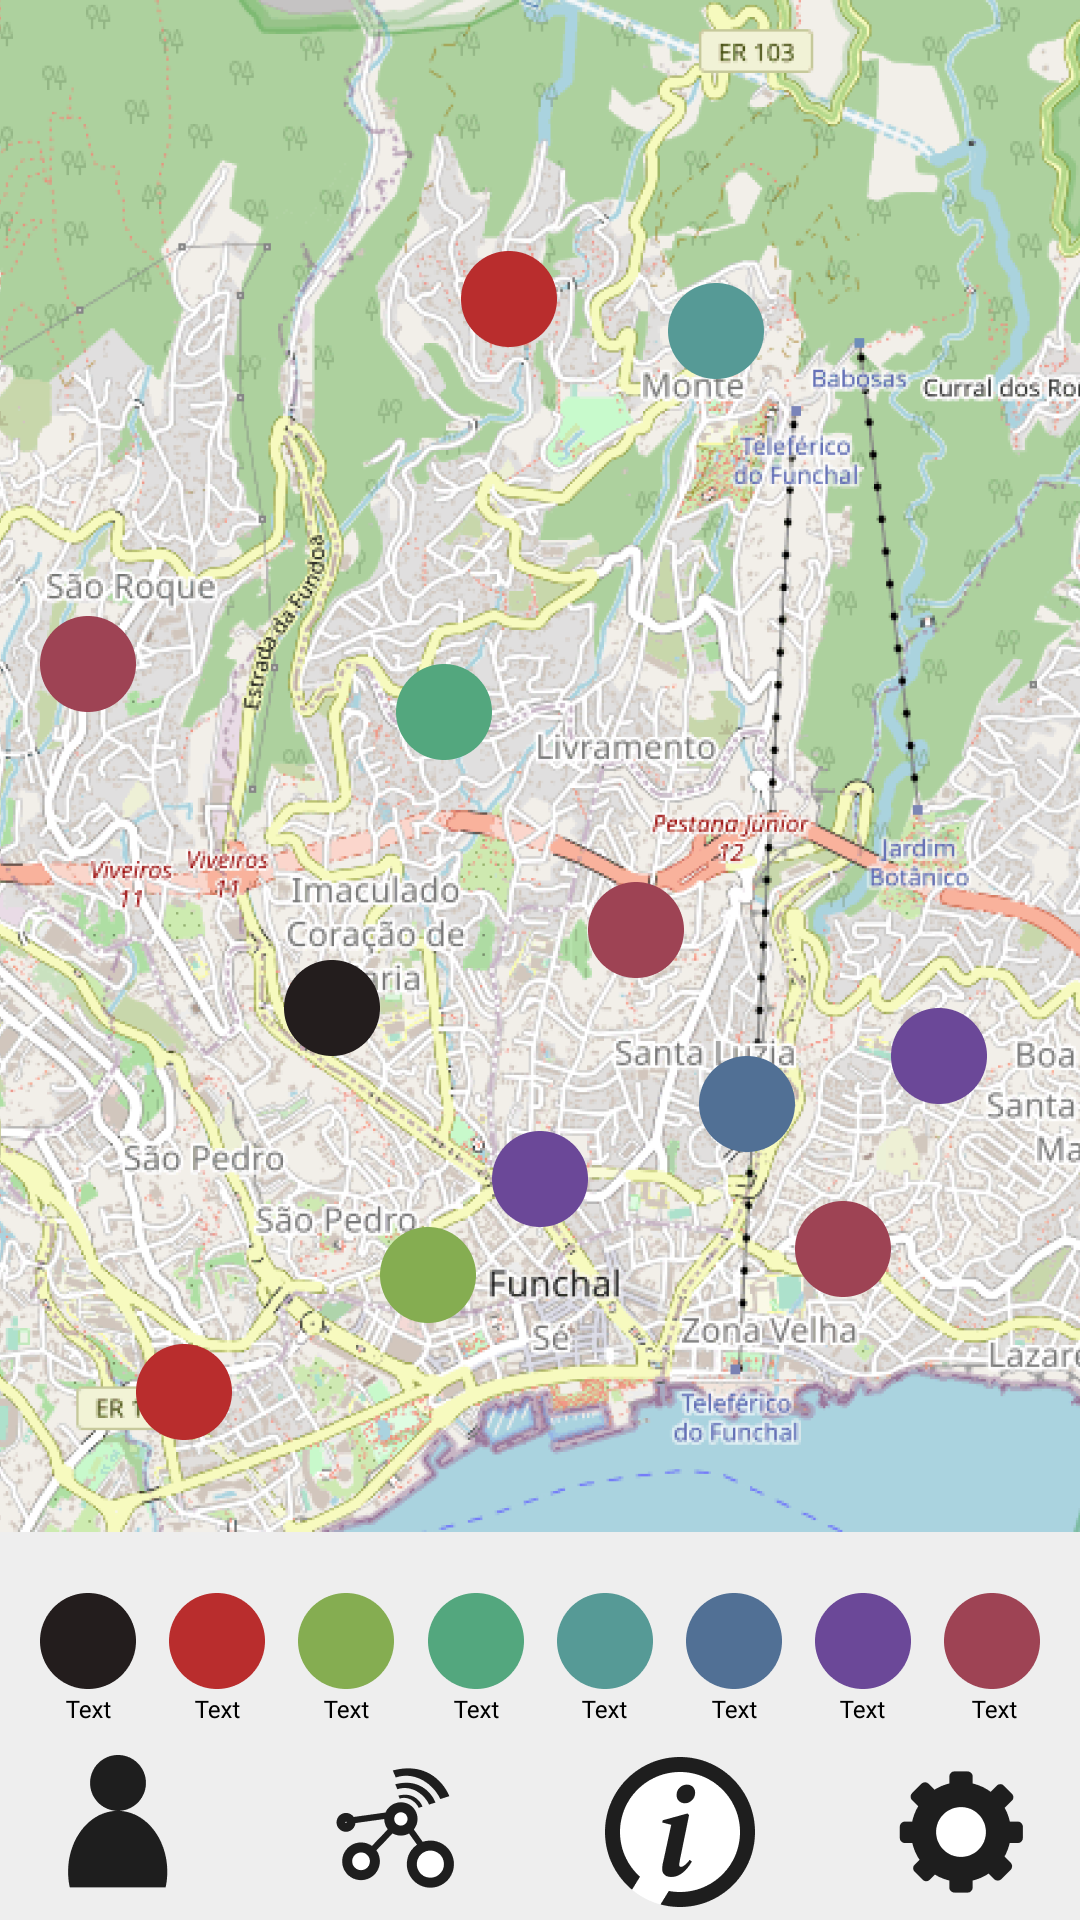
\includegraphics[width=130pt]{../assets/images/low_homepage.png}
        \caption{}
        \label{fig:home}
    \end{subfigure}%
    \begin{subfigure}{0.33\textwidth}
        \centering
        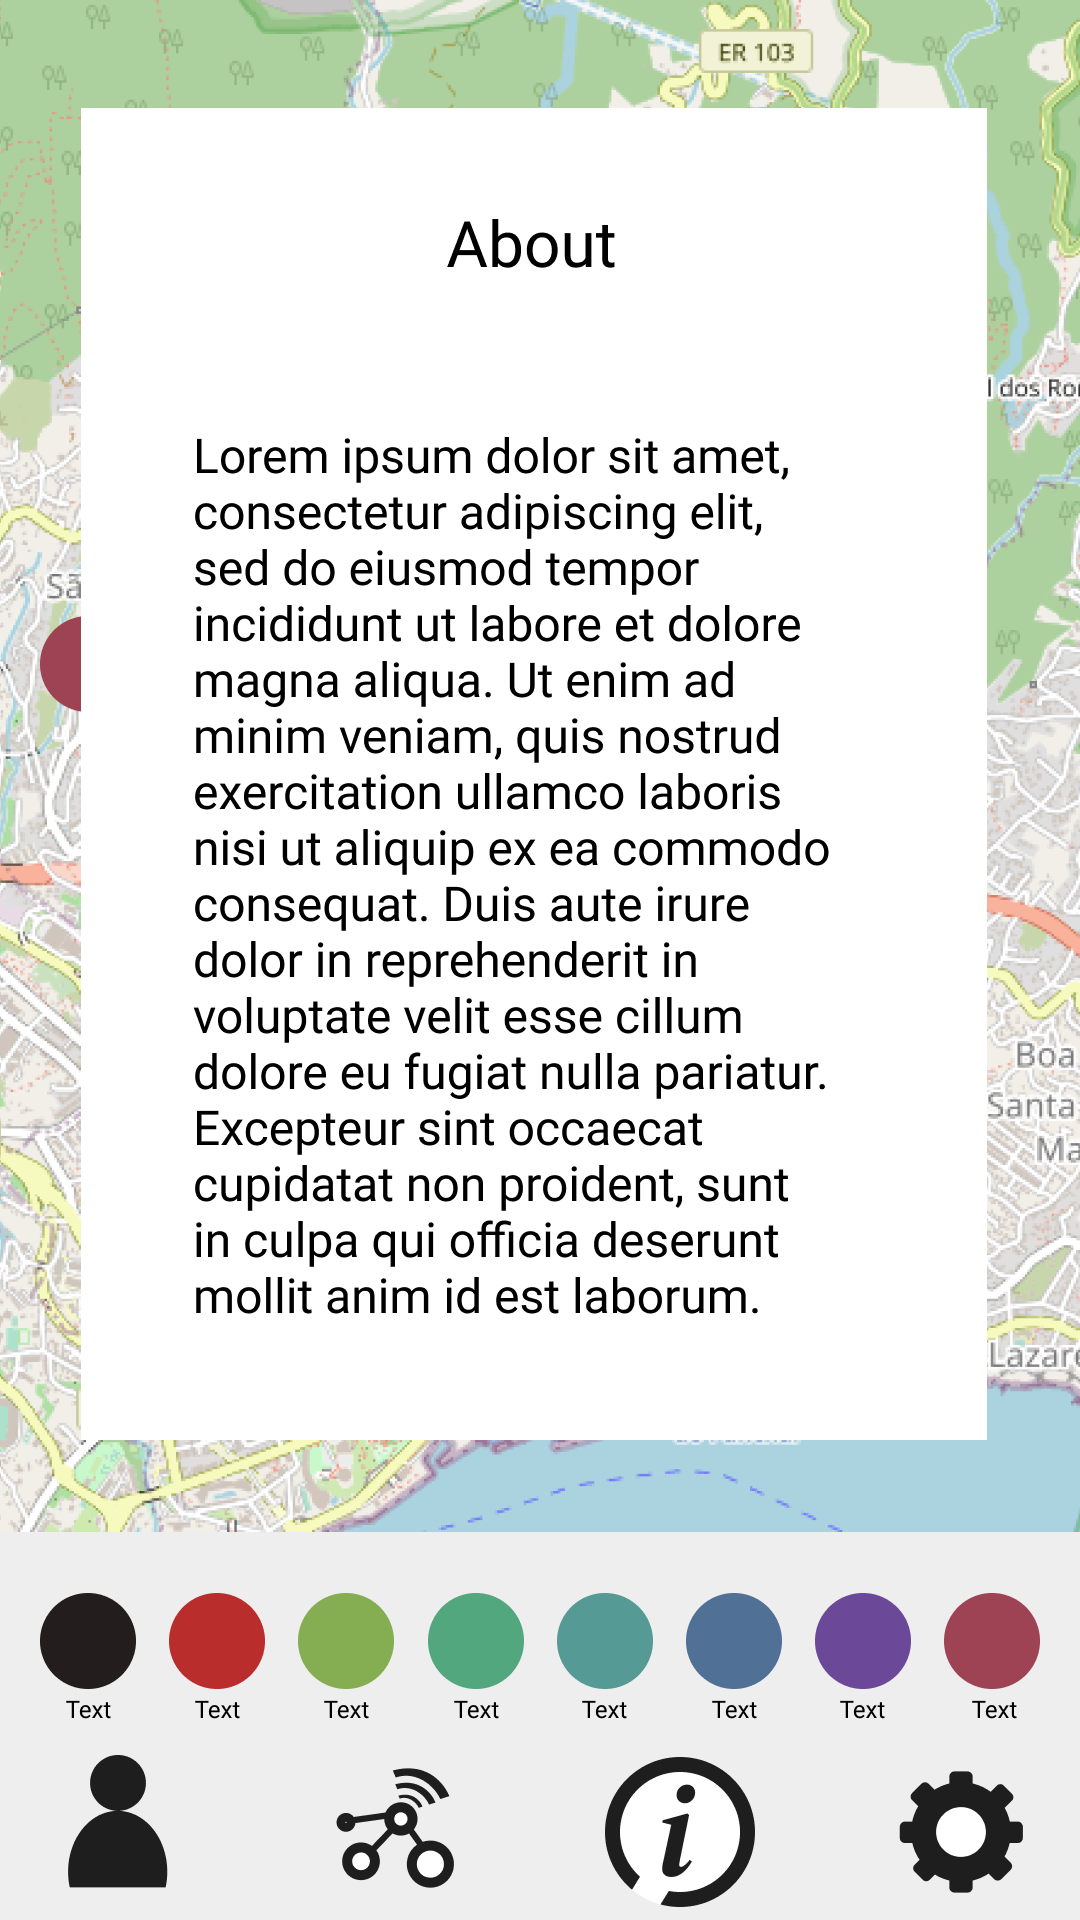
\includegraphics[width=130pt]{../assets/images/low_about.png}
        \caption{}
        \label{fig:about}
    \end{subfigure}%
    \begin{subfigure}{0.33\textwidth}
        \centering
        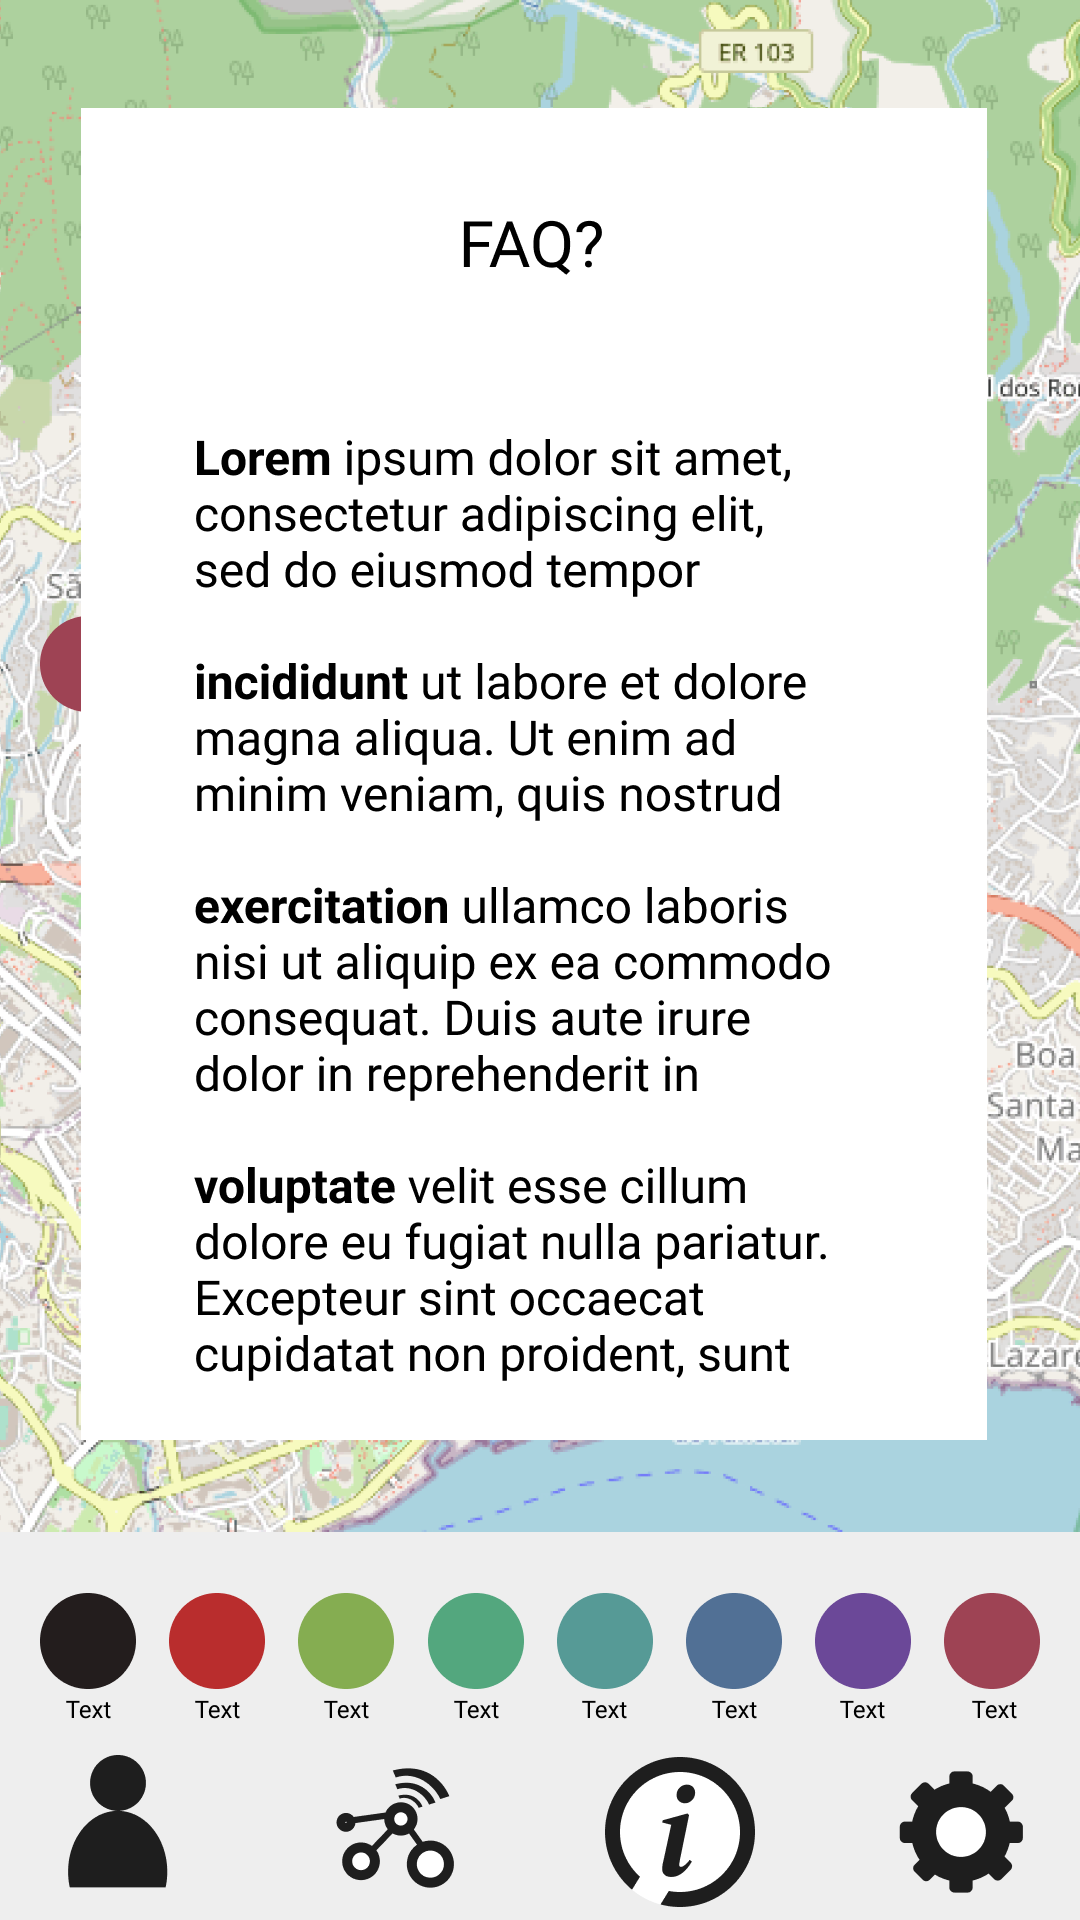
\includegraphics[width=130pt]{../assets/images/low_more_info.png}
        \caption{}
        \label{fig:faq}
    \end{subfigure}%
    \caption{Low level prototype of (a) homepage, (b) about and (c) FAQ pages.}
    \label{fig:lowlevelprototype}
\end{figure}

After creating the software requirements specification, the prototypes were
created. For the creation of the prototypes the following tools were used: Figma
and GIMP.

At first a low level prototype was made in order to understand the
general design and user interaction of the application. Figure \ref{fig:lowlevelprototype}
shows tree pages of the low level prototype, these are the homepage, about
and faq pages, this prototype has a navigation menu on the bottom where the
other pages of the application can be selected along with some information
above the page icons, this information is supposed to be the categories of
the devices, the logic would be that the user could tap one of these categories
and only devices of the category should be displayed on the map. It can
be seen that between the three pages the map stays in the background and
the various pages work like an overlay on the homepage, this would be
changed in subsequent prototype versions.

\begin{figure}
    \centering
    \begin{subfigure}{0.33\textwidth}
        \centering
        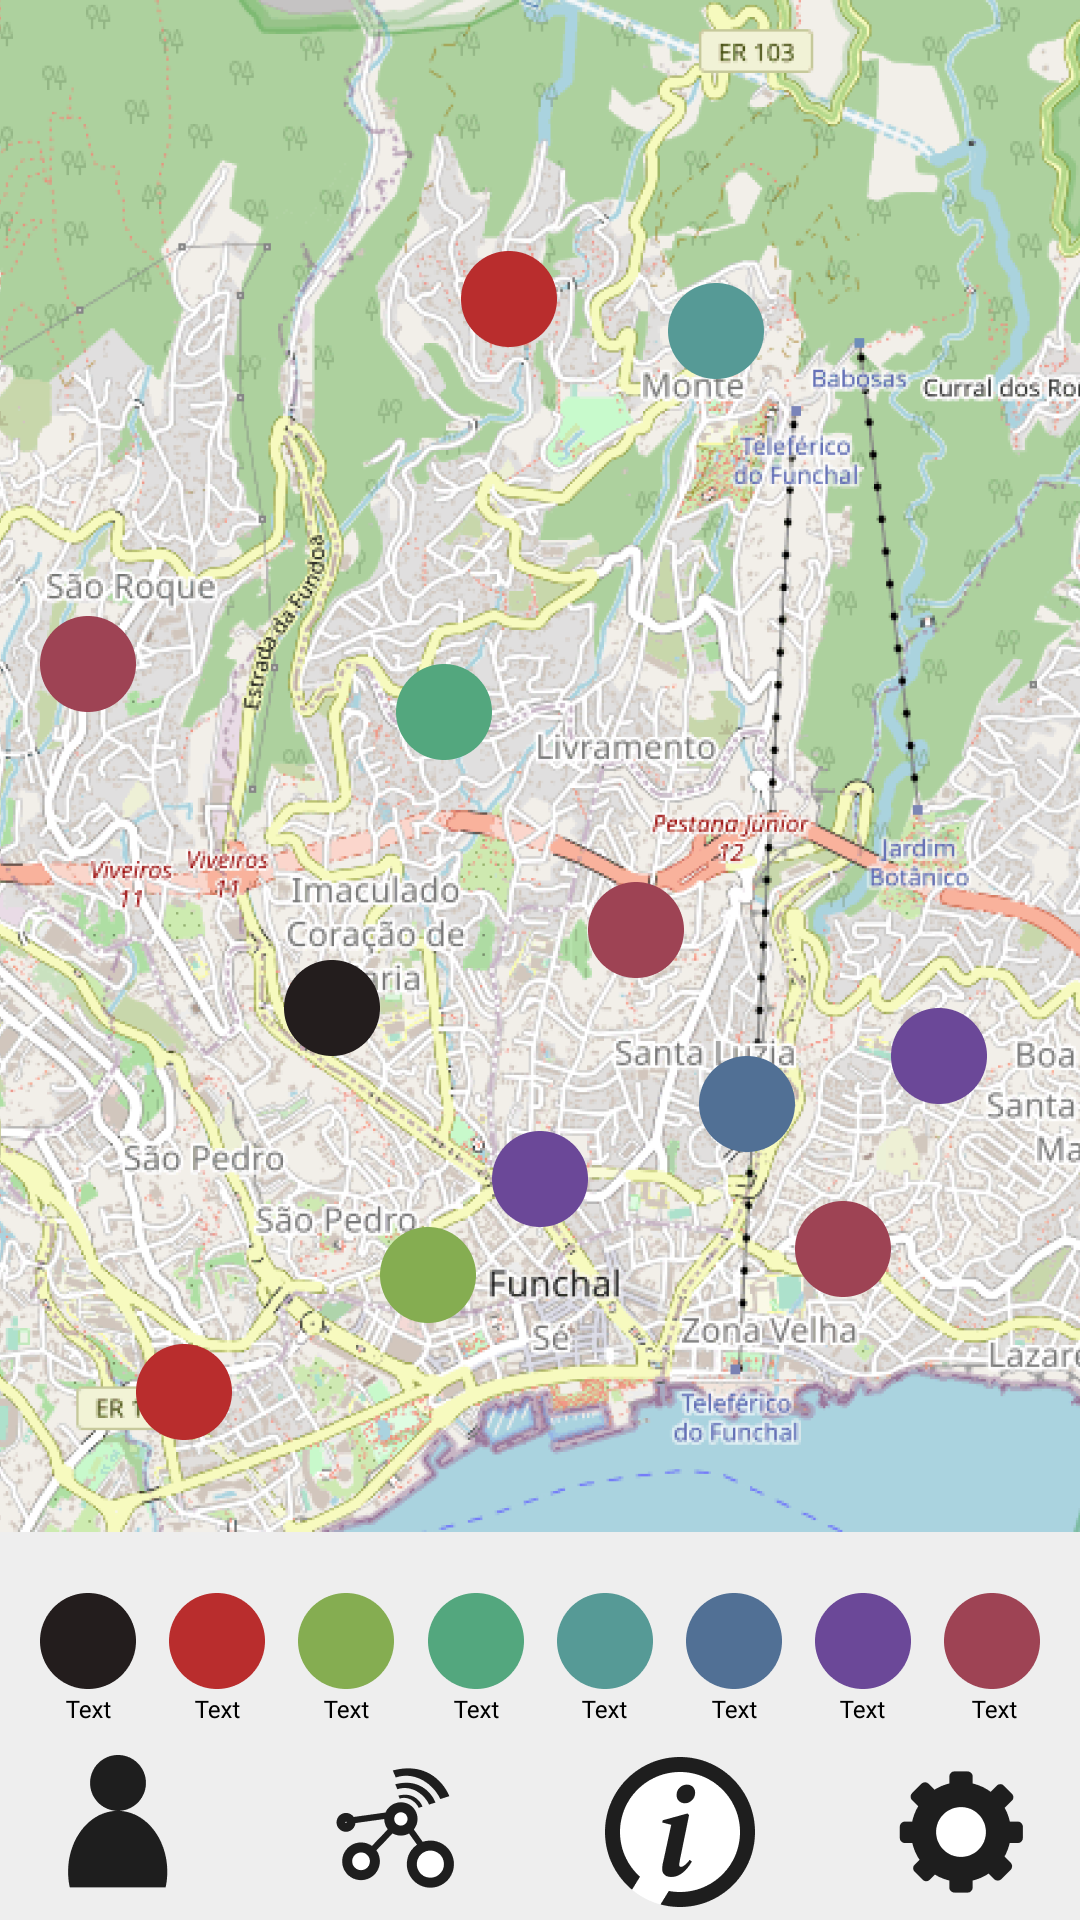
\includegraphics[width=130pt]{../assets/images/low_homepage.png}
        \caption{}
        \label{fig:home}
    \end{subfigure}%
    \begin{subfigure}{0.33\textwidth}
        \centering
        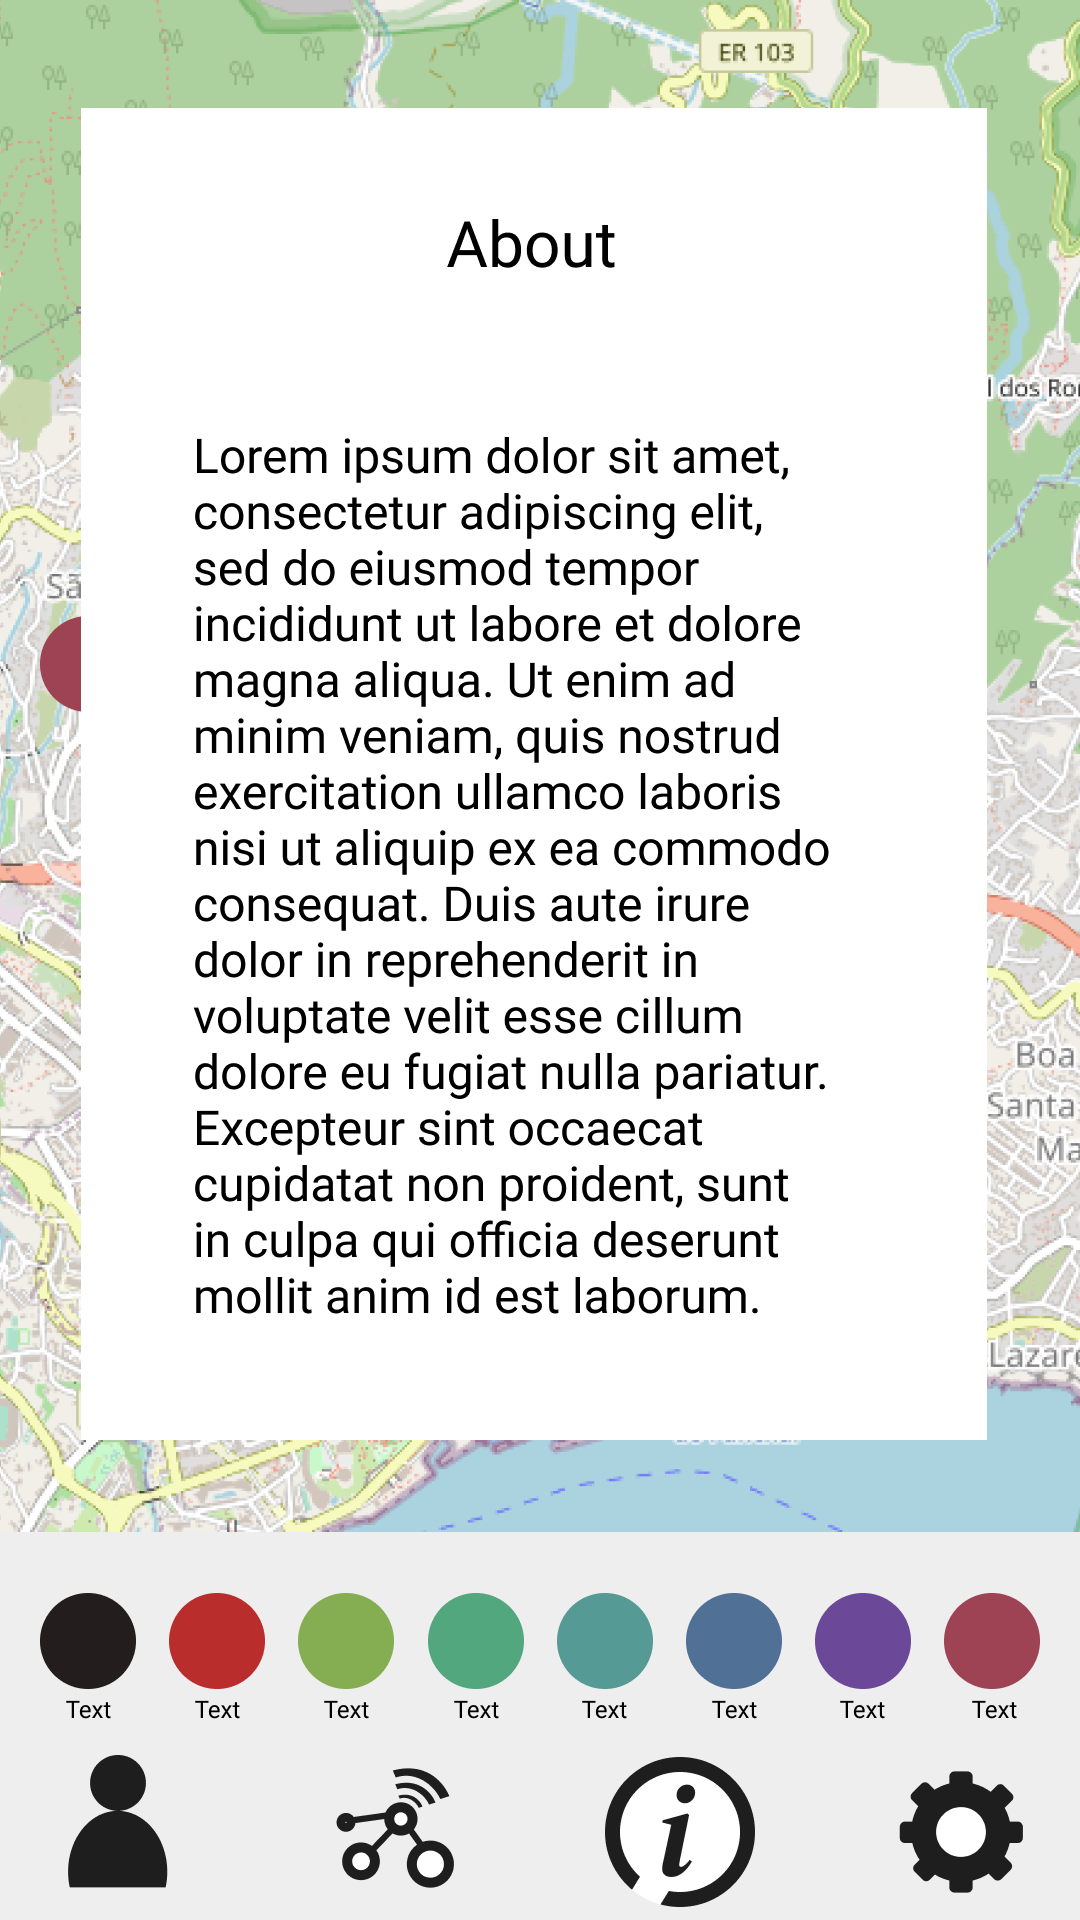
\includegraphics[width=130pt]{../assets/images/low_about.png}
        \caption{}
        \label{fig:about}
    \end{subfigure}%
    \begin{subfigure}{0.33\textwidth}
        \centering
        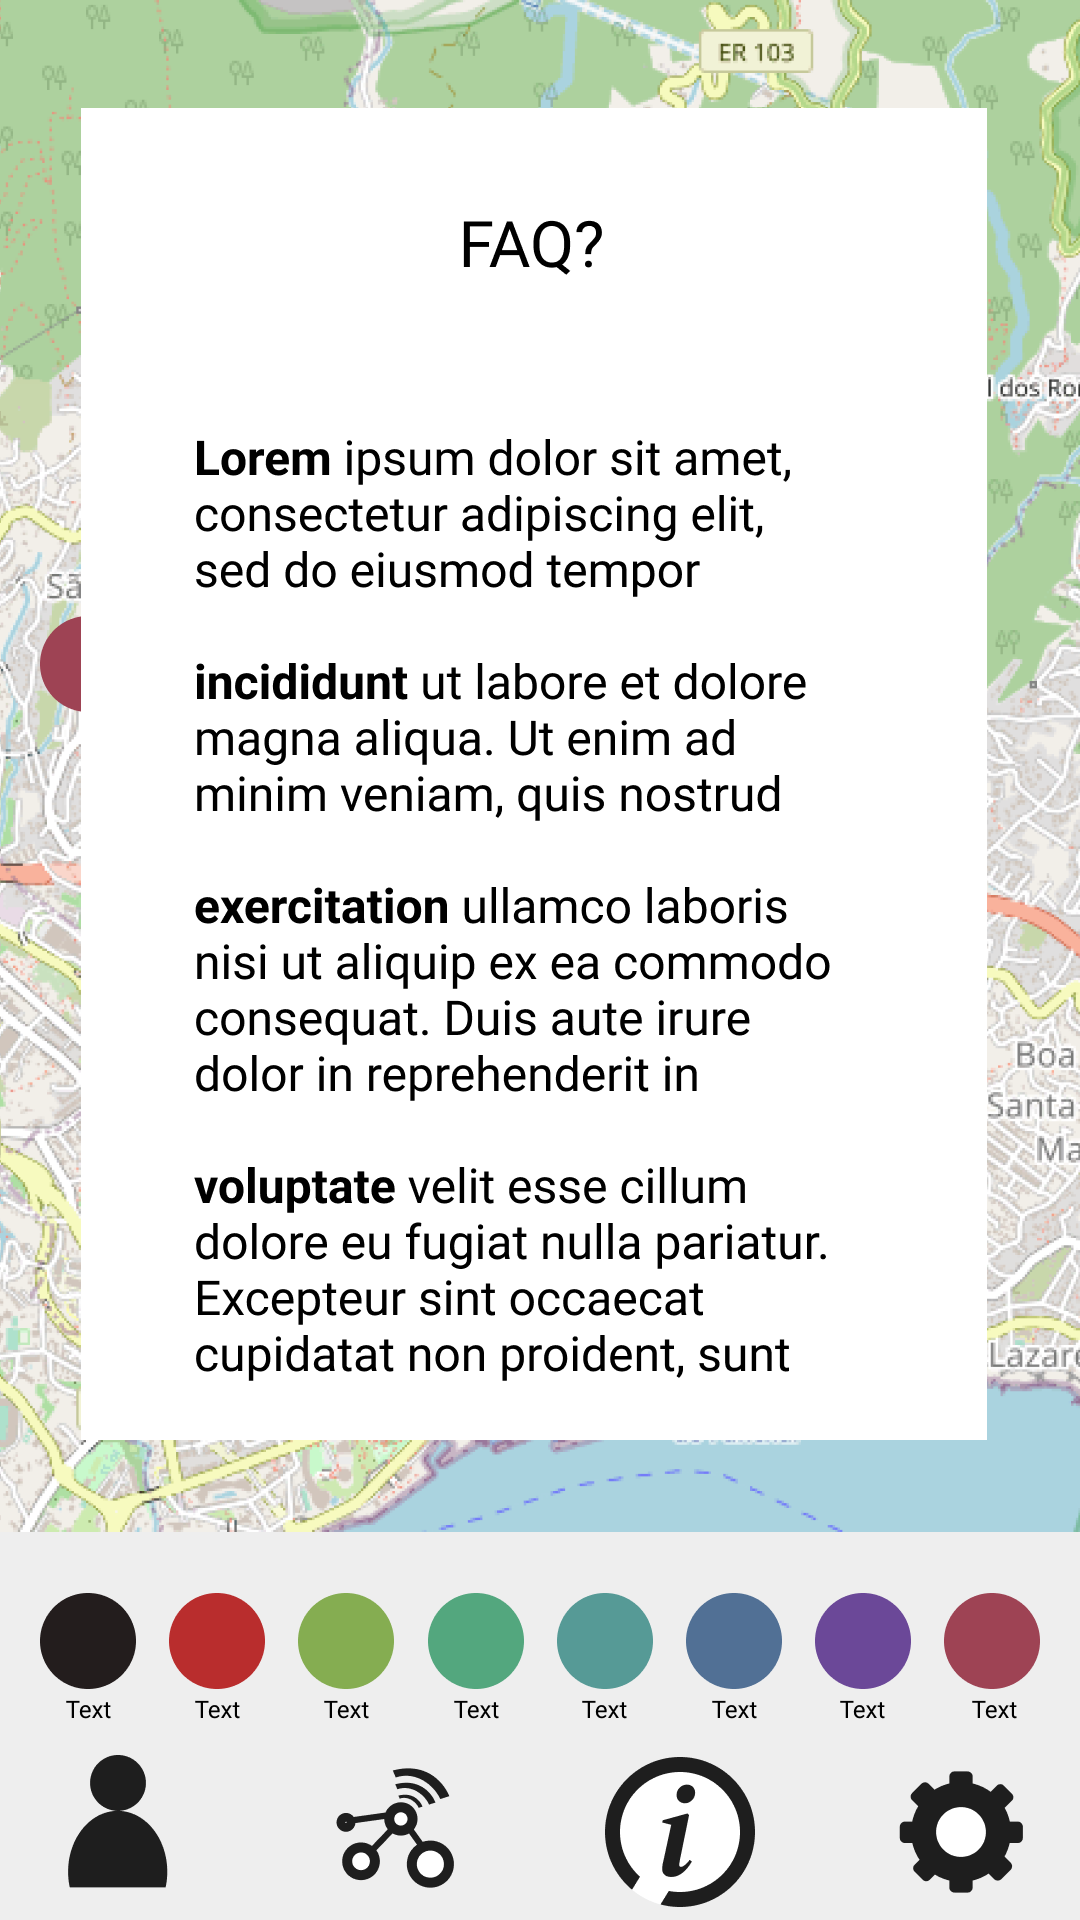
\includegraphics[width=130pt]{../assets/images/low_more_info.png}
        \caption{}
        \label{fig:faq}
    \end{subfigure}%
    \caption{Medium level prototype of (a) homepage, (b) about and (c) FAQ pages.}
    \label{fig:mediumlevelprototype}
\end{figure}

\begin{figure}
    \centering
    \begin{subfigure}{0.33\textwidth}
        \centering
        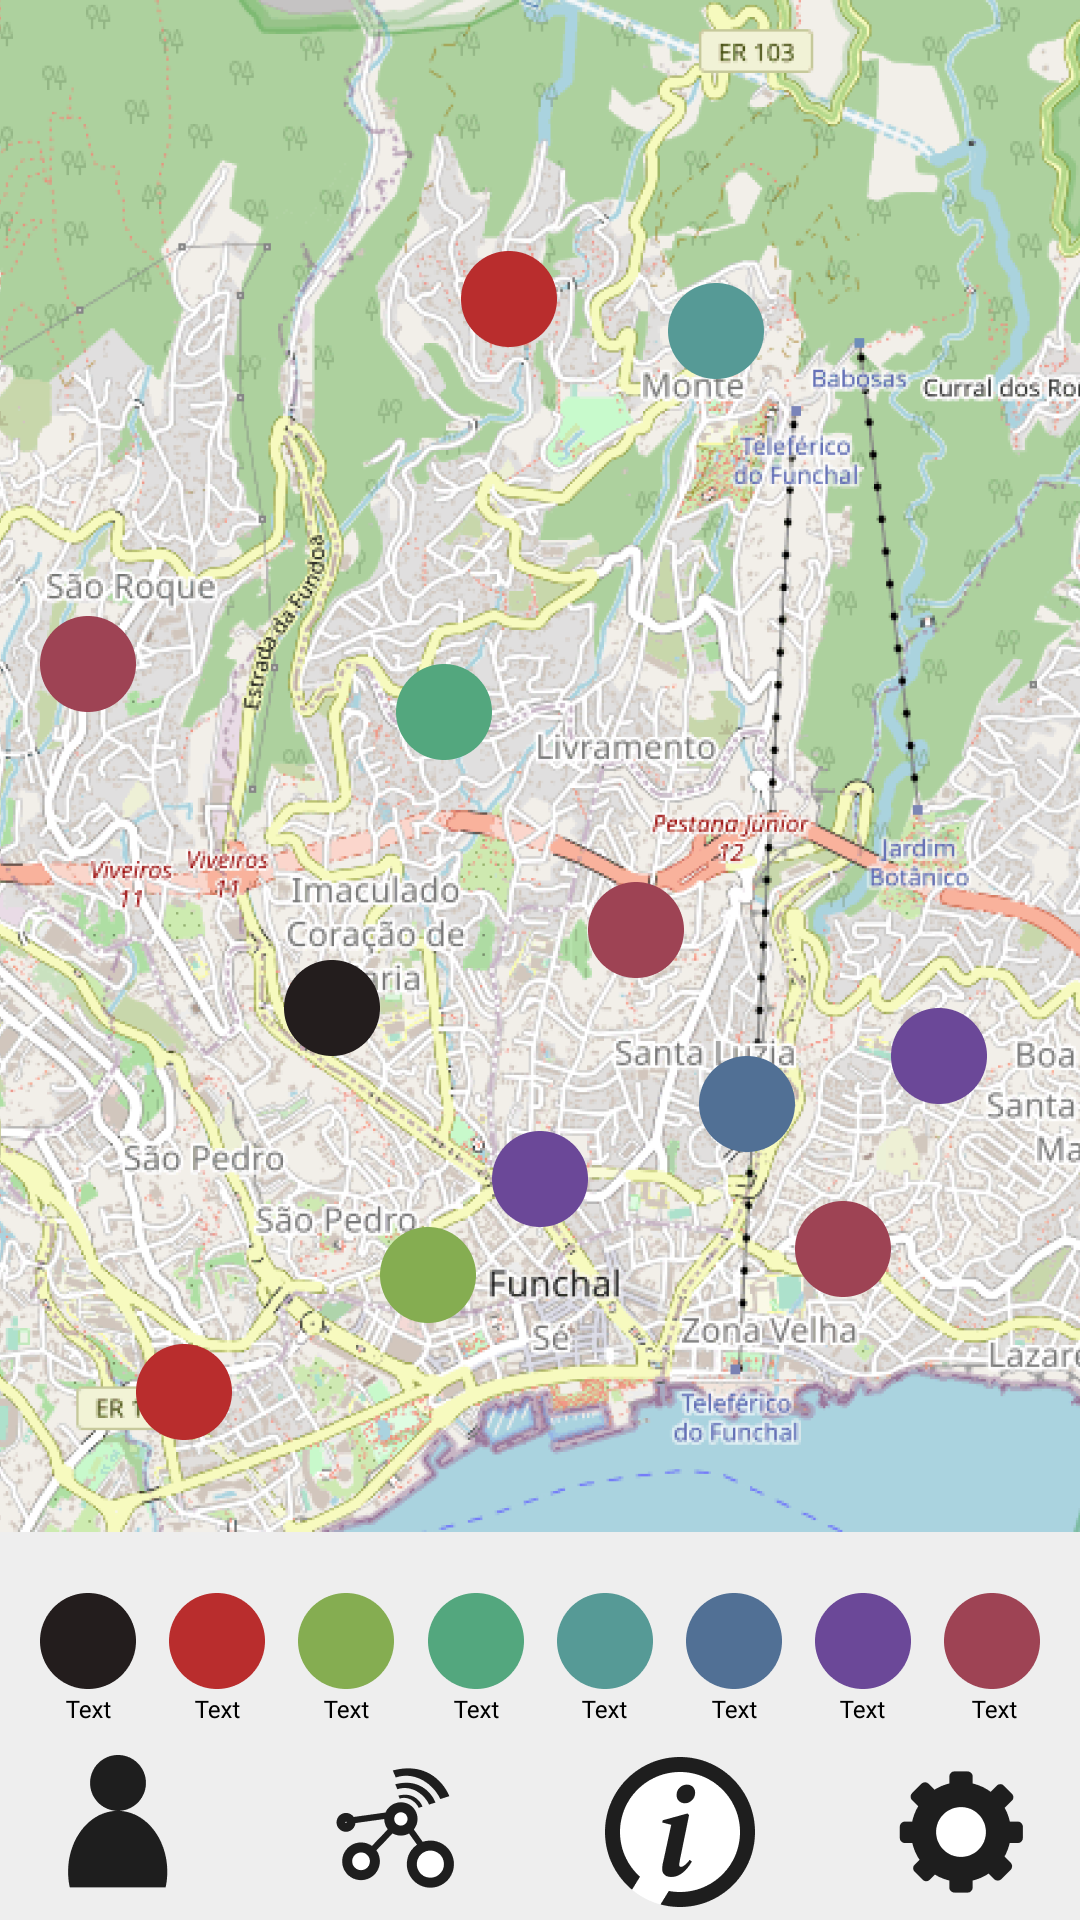
\includegraphics[width=130pt]{../assets/images/low_homepage.png}
        \caption{}
        \label{fig:home}
    \end{subfigure}%
    \begin{subfigure}{0.33\textwidth}
        \centering
        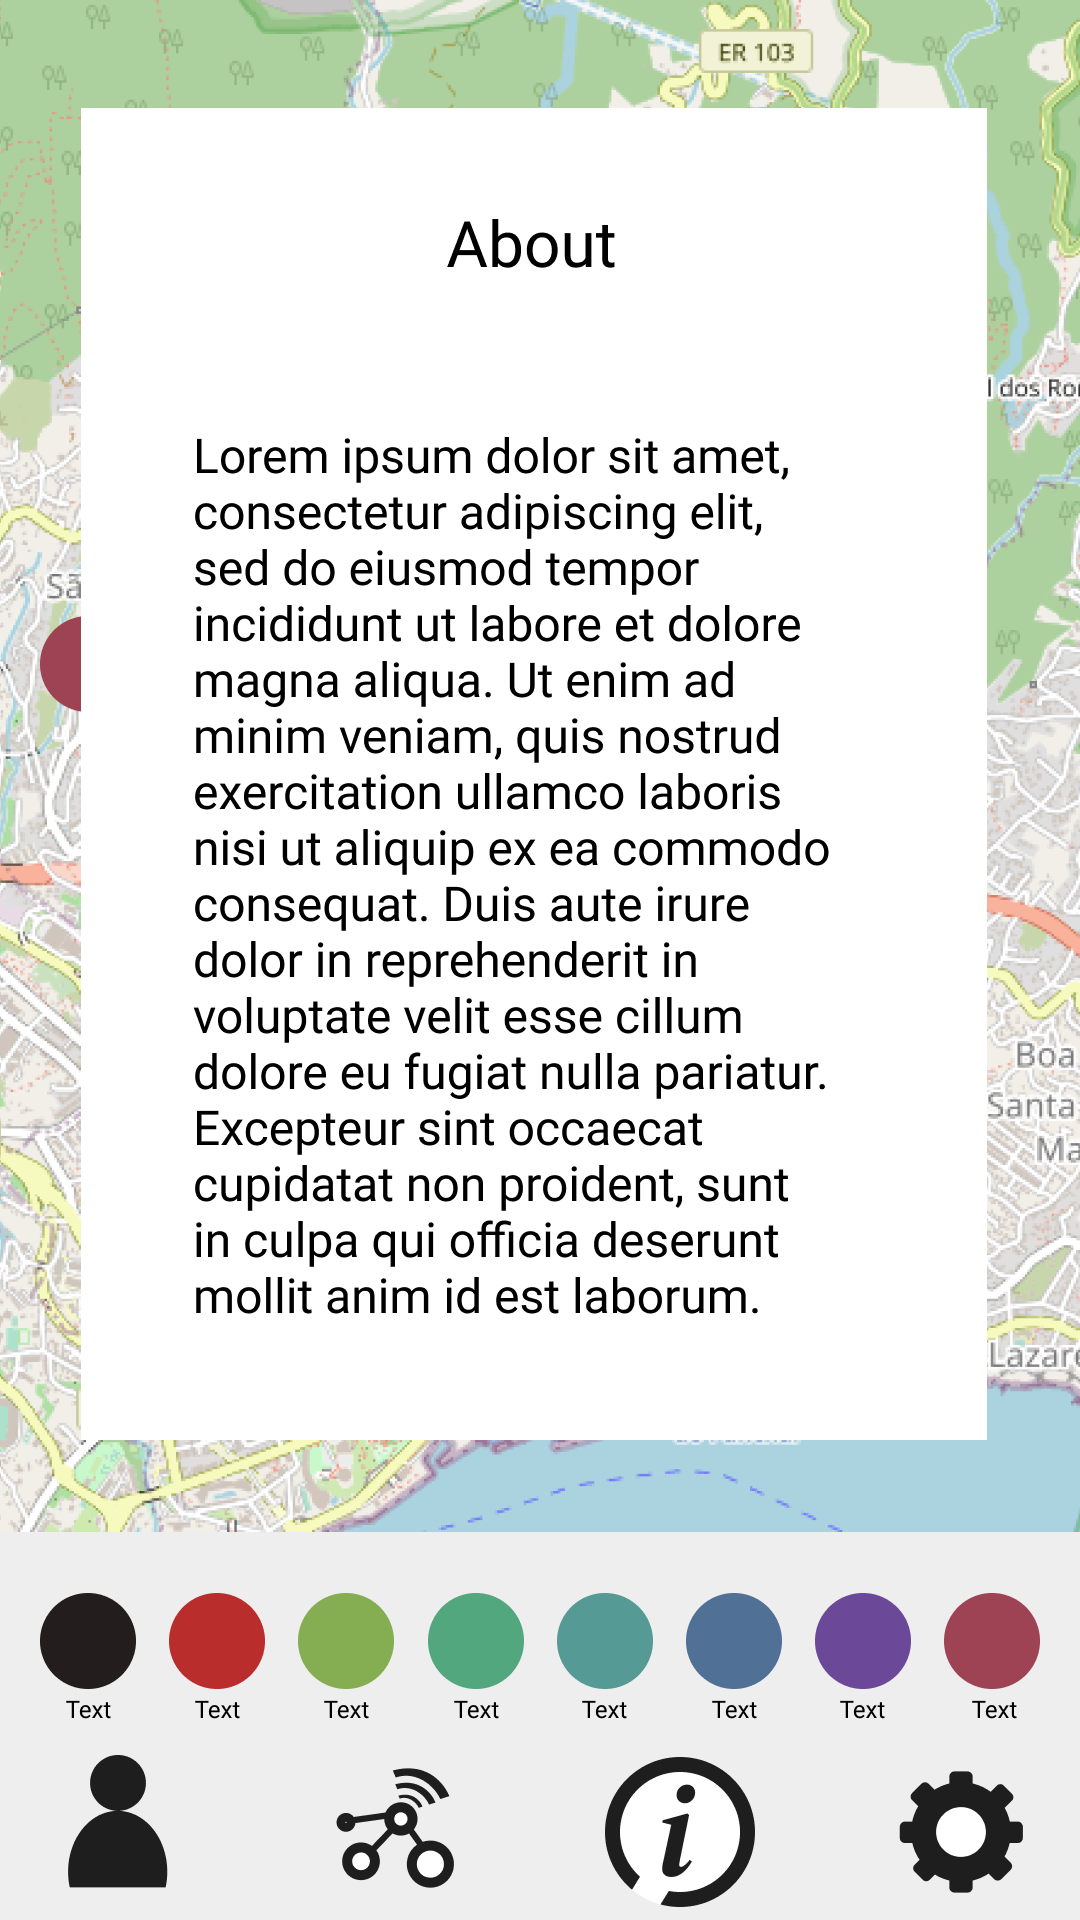
\includegraphics[width=130pt]{../assets/images/low_about.png}
        \caption{}
        \label{fig:about}
    \end{subfigure}%
    \begin{subfigure}{0.33\textwidth}
        \centering
        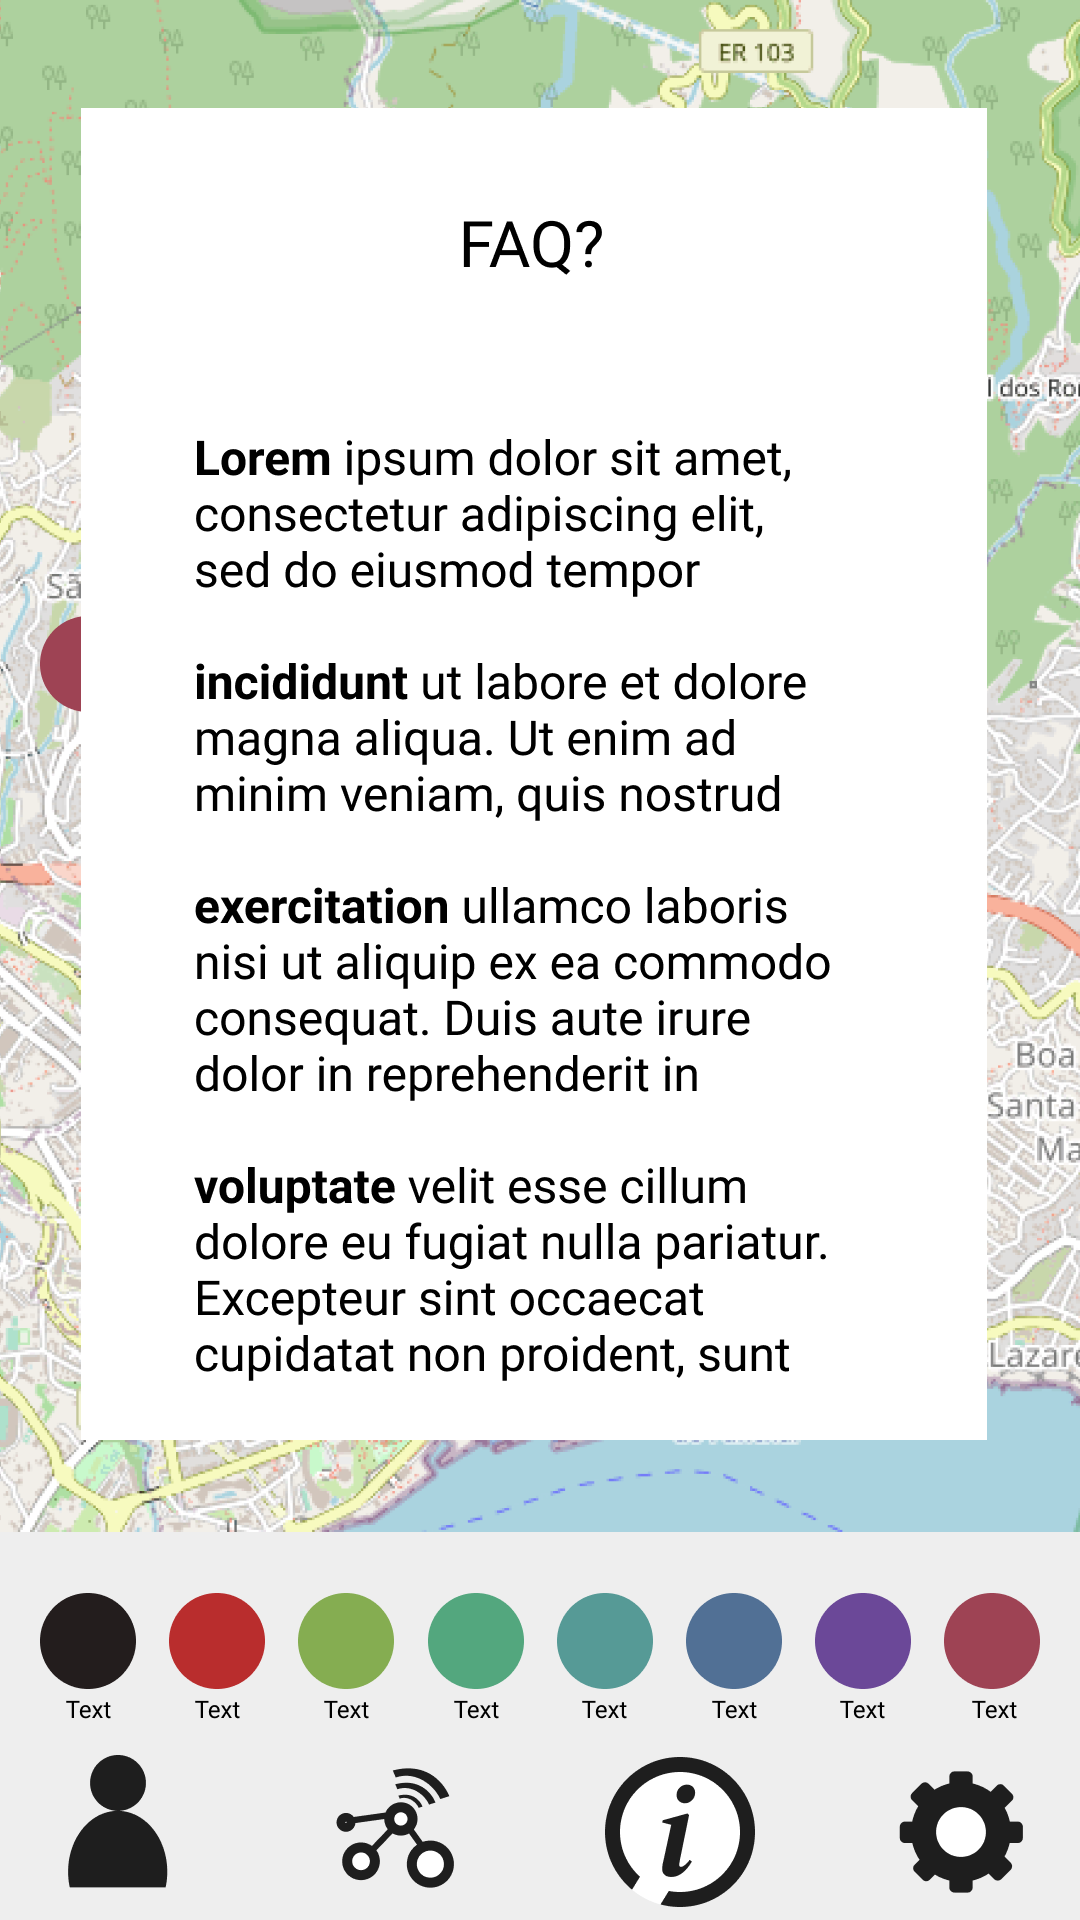
\includegraphics[width=130pt]{../assets/images/low_more_info.png}
        \caption{}
        \label{fig:faq}
    \end{subfigure}%
    \caption{High level prototype of (a) homepage, (b) about and (c) FAQ pages.}
    \label{fig:highlevelprototype}
\end{figure}

\section{Challenges}

One of the most difficult points to accomplish in this thesis was the
questionnaire, not the fact of constructing the questionnaire but of
getting participants. Besides being difficult in itself to get a relatively
high number of participants of participants (a few hundred at least)
to be able to draw conclusions with any high degree of confidence, it was
difficult to get to get the potential participants interested in the topic
at hand, because although it seems that many people value their privacy very
highly and think they should protect it in practice they are not very
interested. This may even be because many people do not have much knowledge
about the Internet of Things, and thus feel that they cannot answer the
questionnaire because it is out of their field of knowledge, another
reason may be that the questionnaire seems a little long, because it
takes on average 15 to 20 minutes to answer, and despite being a topic
of interest the time investment in the questionnaire may be considered
too high. Another point to take into consideration regarding the low
number of participants is the way the questionnaire is written and how
it was advertised, i.e., a very formal or technical language may have
been used both in the construction of the questionnaire and in its
dissemination, and the fact that this is a very niche topic may have
"scared" possible participants. However, it should be noted that also
in the literature that has been carried out there is not a great focus
on conducting questionnaires and the ones that have been conducted have
not only focused on the Internet of Things and also have some monetary
incentive for the participants.

% Um dos pontos mais difíceis de realizar nesta tese foi o questionário,
% não o facto de construir o questionário mas sim de angariar participantes.
% Para além de ser difícil por si só conseguir ter um número de participantes
% relativamente alto (algumas centenas, 500 a 1000) para conseguirmos tirar
% conclusões com algum grau de confiança elevado, foi difícil de conseguir
% com que os possíveis participantes se interessassem no tópico em questão,
% pois apesar de parecer que muitas pessoas valorizem muito a sua privacidade
% e achem que devem a proteger na prática não se interessam muito. Isto até
% pode ser porque muitas pessoas não tenham muito conhecimento a nível da
% Internet of Things, e assim acharem que não conseguem responder ao questionário
% por ser fora do seu campo de conhecimento, outra razão pode o questionário
% parecer um pouco longo, pois demora em média 15 a 20 minutos para responder,
% e apesar de até ser um tópico de interesse o investimento de tempo no
% questionário pode ser considerado muito elevado. Outro ponto a ter em consideração
% em relação ao baixo número de participantes é a forma como o questionário
% está escrito e como este foi divulgado, isto é, pode ter sido usado
% uma linguagem muito formal ou técnica tanto na construção do mesmo como
% também na sua divulgação e juntado ao facto de este ser um tópico muito niche
% pode ter "assustando" possíveis participantes. Contudo é de notar que
% também na literatura que tem vindo a ser realizada não há um grande foco
% na realização de questionários e os que têm sido realizados não têm se
% focado somente na Internet of Things e têm também algum incentivo monetário
% para os participantes.

    \clearpage
    % SPDX-License-Identifier: CC-BY-4.0
%
% Copyright (c) 2023 Nelson Vieira
%
% @author Nelson Vieira <2080511@student.uma.pt>
% @contributor Mary Barreto <mary.barreto@staff.uma.pt>
% @license CC-BY-4.0 <https://creativecommons.org/licenses/by/4.0/legalcode.txt>
\section{Discussion}\label{section:discussion}

\par
This chapter serves to discusses the main takeaways found in the literature
review and address the results of the questionnaire and the usability tests,
and any other interesting remarks found during the course of this work. The
research questions that were posed in Chapter \ref{introduction} will also
be addressed.

\subsection{SLR Findings}

There has been a rising interest by research papers in addressing privacy
issues or challenges in the Internet of Things, at least since 2015-2016
where the number or papers jumped from 11 600 in 2015 to 19 400 in 2016
and rising since then until reaching a peak of 74 400 in 2020 and slightly
declining since then, and at least until August of 2023 there have been
around 36 000 papers published, according to the data seen in Figure \ref{fig:iotprivacy_papers}.

\begin{figure}
    \begin{center}
        \pgfkeys{/pgf/number format/1000 sep={\,}}
        \begin{tikzpicture}
            \begin{axis}[
                width=15cm,
                height=8cm,
                xmin=2010,
                xmax=2023,
                ymin=0,
                ymax=74400,
                xlabel=Year,
                ylabel=Papers,
                axis x line=bottom,
                axis y line=left,
                nodes near coords={\pgfmathprintnumber[fixed]\pgfplotspointmeta}
            ]
            \addplot[draw=SkyBlue!70!white,samples=100,fill=SkyBlue!70!white,fill opacity=0.1] coordinates {(2010,1040) (2011,1520) (2012,2650) (2013,4150) (2014,6650) (2015,11600) (2016,19400) (2017,31100) (2018,48300) (2019,60800) (2020,74400) (2021,72300) (2022,67700) (2023,36000)}\closedcycle;
            \addplot[blue!40!black,thick,samples=100,domain=2010:2023] coordinates {(2010,1040) (2011,1520) (2012,2650) (2013,4150) (2014,6650) (2015,11600) (2016,19400) (2017,31100) (2018,48300) (2019,60800) (2020,74400) (2021,72300) (2022,67700) (2023,36000)};
            \end{axis}
        \end{tikzpicture}
        \caption{Distribution of papers, per year since 2010, on privacy in the Internet of Things, based on Google Scholar database results.}
        \label{fig:iotprivacy_papers}
    \end{center}
\end{figure}

Figure \ref{fig:privacy_keywords_papers} depicts the number of publications
per topic in multiple databases, all of which are still related to the main
theme of privacy in the \DTLassign{acronyms}{14}{\acronym=Acronym}\hyperlink{\acronym}{\acronym}, particularly Google Scholar, \DTLassign{acronyms}{2}{\acronym=Acronym}\hyperlink{\acronym}{\acronym}, and CORE. This
data is from papers since 2020, the database with the most papers is Google Scholar
followed by the distant second \DTLassign{acronyms}{2}{\acronym=Acronym}\hyperlink{\acronym}{\acronym} and finally
CORE with the smallest number of papers. Around 249000 papers exist discussing privacy
in the \DTLassign{acronyms}{14}{\acronym=Acronym}\hyperlink{\acronym}{\acronym} in Google Scholar, 20641 papers on CORE and 8014 on \DTLassign{acronyms}{2}{\acronym=Acronym}\hyperlink{\acronym}{\acronym}, from these papers
the most researched topic has been security with around 196000 papers on Google Scholar,
17738 on CORE and 5600 on \DTLassign{acronyms}{2}{\acronym=Acronym}\hyperlink{\acronym}{\acronym}. This data cannot be accepted at face value because
searches on these databases are conducted using keywords, these keywords may occur
in the title of the work or on the content, but this does not imply that the work
is about keywords in general, rather, it simply indicates that the keywords appear
on the work. But it can represent a rough estimate of what is being researched.
Other databases were used in course of the research like Semantic Scholar,
Baidu Scholar and RefSeek but these databases do not have good
filters for advanced searching and/or have a small number of papers.

There is a big focus on security, AI and blockchain in recent literature,
specially from 2020 onward. Some studies \cite{dadkhah2020publications, duygu2023analysis} have
focused on this type of analysis.

\begin{figure}[H]
    \begin{center}
        \pgfkeys{/pgf/number format/1000 sep={\,}}
        \begin{tikzpicture}
            \begin{axis}[
                width=10cm,
                height=16cm,
                xbar,
                xmin=0,
                symbolic y coords={Privacy in the IoT,Privacy paradox in the IoT,Differential privacy in the IoT,Machine learning and privacy in the IoT,Deep learning and privacy in the IoT,Blockchain and privacy in the IoT,Security and privacy in the IoT,Privacy framework/architecture in the IoT,Privacy literacy in the IoT,Artificial intelligence and privacy in the Internet of things},
                ytick=data,
                yticklabels={
                    Privacy\\in the IoT,
                    Privacy paradox\\in the IoT,
                    Differential privacy\\in the IoT,
                    Machine learning and\\privacy in the IoT,
                    Deep learning and\\privacy in the IoT,
                    Blockchain and privacy\\in the IoT,
                    Security and privacy\\in the IoT,
                    Privacy framework/architecture\\in the IoT,
                    Privacy literacy\\in the IoT,
                    Artificial intelligence and\\privacy in the Internet of things,
                },
                yticklabel style={align=right},
                bar width=8pt,
                axis x line=bottom,
                axis y line=left,
                xticklabel style={/pgf/number format/fixed},
                enlarge y limits=0.1,
                nodes near coords={\pgfmathprintnumber[fixed]\pgfplotspointmeta},
                legend style={at={(0.5,-0.1)},anchor=north},
                % ticklabel style={font=\tiny},
            ]
                \addplot[ForestGreen!30!black,fill=ForestGreen!60!white] coordinates {(249000,Privacy in the IoT) (1850,Privacy paradox in the IoT) (9520,Differential privacy in the IoT) (109000,Machine learning and privacy in the IoT) (75100,Deep learning and privacy in the IoT) (73300,Blockchain and privacy in the IoT) (196000,Security and privacy in the IoT) (99900,Privacy framework/architecture in the IoT) (23900,Privacy literacy in the IoT) (166000,Artificial intelligence and privacy in the Internet of things)};
                \addlegendentry{Google Scholar}
                \addplot[YellowOrange!30!black,fill=YellowOrange!60!white] coordinates {(8014,Privacy in the IoT) (18,Privacy paradox in the IoT) (229,Differential privacy in the IoT) (1401,Machine learning and privacy in the IoT) (554,Deep learning and privacy in the IoT) (1650,Blockchain and privacy in the IoT) (5600,Security and privacy in the IoT) (2724,Privacy framework/architecture in the IoT) (29,Privacy literacy in the IoT) (1247,Artificial intelligence and privacy in the Internet of things)};
                \addlegendentry{BASE}
                \addplot[BlueViolet!30!black,fill=BlueViolet!60!white] coordinates {(20641,Privacy in the IoT) (384,Privacy paradox in the IoT) (1020,Differential privacy in the IoT) (11255,Machine learning and privacy in the IoT) (6643,Deep learning and privacy in the IoT) (6663,Blockchain and privacy in the IoT) (17738,Security and privacy in the IoT) (16327,Privacy framework/architecture in the IoT) (2611,Privacy literacy in the IoT) (10868,Artificial intelligence and privacy in the Internet of things)};
                \addlegendentry{CORE}
            \end{axis}
        \end{tikzpicture}
        \caption{Distribution of papers on privacy in IoT, since 2020, by keyword searches on Google Scholar, BASE and CORE databases.}
        \label{fig:privacy_keywords_papers}
    \end{center}
\end{figure}

Chapter \ref{section:state_of_the_art} discussed many works that addressed privacy challenges in the
\DTLassign{acronyms}{14}{\acronym=Acronym}\hyperlink{\acronym}{\acronym} and some that proposed approaches to address these issues. The current chapter assesses
different aspects of the included papers including their general information,
purpose, intended application, issues that still exist, and any other comments
that should be taken into account.

Table \ref{table:literature_overview} displays general information about the
papers that were included \cite{wilson2012unpacking, warshaw2015can, lee2015privacy, acquisti2007can, knijnenburg2013dimensionality, wakefield2013influence, flender2012type, dienlin2015privacy, baek2014solving, taddicken2014privacy, norberg2007privacy, kokolakis2017privacy, brandimarte2013misplaced, xie2019consumers, SCHWAIG20131, sannon2018privacy, ZhaoSurvey, zhao2020local, Gupta2022Privacy, Kuhtreiber2022survey, sicari2015security, LinSurvey, yang2022overview, zubaydi2023leveraging, khanna2020internet, tzafestas2018ethics, ziegeldorf2014privacy, naeini2017privacy, koohang2022internet, SkirpanPrivacy, WEBER2015618, FabianoInternet, weber2010internet, hadzovic2023path, SunSecure, xiong2018defending, AntunesFederated, opara2022framework, perera2020designing, zhang2017privacy, zhang2019security, yu2018blockchain, AliIoT, ColnagoInforming, FengDesign, DasPersonalized, ZhuIntegrating, electronics12122589, KumarLTE}.
It is discernible that 22\% of the total papers were published in 2022 \cite{ZhaoSurvey, Gupta2022Privacy, Kuhtreiber2022survey, yang2022overview, zubaydi2023leveraging, koohang2022internet, SkirpanPrivacy, SunSecure, AntunesFederated, opara2022framework, ZhuIntegrating},
while 12\% of the papers were published in 2017 \cite{kokolakis2017privacy, LinSurvey, naeini2017privacy, FabianoInternet, zhang2017privacy, AliIoT},
with 12\% as well as in 2018 \cite{sannon2018privacy, tzafestas2018ethics, xiong2018defending, yu2018blockchain, DasPersonalized, Qu2018Privacy}
and in 2015 \cite{warshaw2015can, lee2015privacy, dienlin2015privacy, sicari2015security, WEBER2015618, perera2015big},
there were 8\% of papers published in 2013 \cite{knijnenburg2013dimensionality, wakefield2013influence, brandimarte2013misplaced, SCHWAIG20131},
with the same percentage in 2014 \cite{baek2014solving, taddicken2014privacy, ziegeldorf2014privacy, KumarLTE}
and in 2020 \cite{zhao2020local, khanna2020internet, perera2020designing, ColnagoInforming},
the remaining 18\% of papers were published between the years 2010 \cite{weber2010internet},
2012 \cite{wilson2012unpacking, flender2012type}, 2019 \cite{xie2019consumers, zhang2019security},
2021 \cite{FengDesign} and 2023 \cite{hadzovic2023path, electronics12122589},
with the exception of a small percentage of 2.08\% being published in 2007 \cite{norberg2007privacy}.
Overall, 38\% of the literature originate from the \DTLassign{acronyms}{31}{\acronym=Acronym}\hyperlink{\acronym}{\acronym} \cite{wilson2012unpacking, warshaw2015can, knijnenburg2013dimensionality, wakefield2013influence, norberg2007privacy, brandimarte2013misplaced, xie2019consumers, SCHWAIG20131, sannon2018privacy, Gupta2022Privacy, naeini2017privacy, koohang2022internet, SkirpanPrivacy, xiong2018defending, opara2022framework, ColnagoInforming, FengDesign, DasPersonalized, KumarLTE},
10\% originate from China \cite{LinSurvey, SunSecure, zhang2017privacy, zhang2019security, yu2018blockchain},
10\% are from Germany \cite{flender2012type, dienlin2015privacy, taddicken2014privacy, Kuhtreiber2022survey, ziegeldorf2014privacy}
and 42\% are spread across 13 different countries \cite{lee2015privacy, baek2014solving, kokolakis2017privacy, ZhaoSurvey, zhao2020local, sicari2015security, yang2022overview, zubaydi2023leveraging, khanna2020internet, tzafestas2018ethics, WEBER2015618, FabianoInternet, weber2010internet, hadzovic2023path, AntunesFederated, perera2020designing, AliIoT, ZhuIntegrating, electronics12122589}.
The majority of the included papers, 74\% \cite{lee2015privacy, knijnenburg2013dimensionality, wakefield2013influence, dienlin2015privacy, baek2014solving, taddicken2014privacy, norberg2007privacy, kokolakis2017privacy, brandimarte2013misplaced, xie2019consumers, SCHWAIG20131, ZhaoSurvey, zhao2020local, Gupta2022Privacy, Kuhtreiber2022survey, sicari2015security, LinSurvey, yang2022overview, zubaydi2023leveraging, khanna2020internet, tzafestas2018ethics, ziegeldorf2014privacy, koohang2022internet, WEBER2015618, weber2010internet, hadzovic2023path, SunSecure, AntunesFederated, perera2020designing, zhang2017privacy, zhang2019security, yu2018blockchain, DasPersonalized, ZhuIntegrating, electronics12122589},
are published in journals, while 24\% are published in conferences \cite{wilson2012unpacking, warshaw2015can, flender2012type, sannon2018privacy, naeini2017privacy, FabianoInternet, xiong2018defending, opara2022framework, AliIoT, ColnagoInforming, FengDesign, KumarLTE},
and 2\% in a magazine \cite{SkirpanPrivacy}.
The publishers' information is provided so that the database of origin
can be easily accessed. The ACM database \cite{warshaw2015can, sannon2018privacy, ZhaoSurvey, SkirpanPrivacy, SunSecure, AntunesFederated, opara2022framework, zhang2019security, AliIoT, ColnagoInforming, FengDesign, ZhuIntegrating, KumarLTE}
provides 26\% of all publications, followed by Elsevier \cite{lee2015privacy, knijnenburg2013dimensionality, wakefield2013influence, baek2014solving, kokolakis2017privacy, SCHWAIG20131, Kuhtreiber2022survey, sicari2015security, koohang2022internet, WEBER2015618, weber2010internet, perera2020designing}
with 24\%, IEEE \cite{zhao2020local, Gupta2022Privacy, LinSurvey, FabianoInternet, hadzovic2023path, xiong2018defending, zhang2017privacy, yu2018blockchain, DasPersonalized}
with 22\%, MDPI \cite{zubaydi2023leveraging, tzafestas2018ethics, electronics12122589}
with 6\% and Wiley \cite{dienlin2015privacy, norberg2007privacy, ziegeldorf2014privacy}
with the same percentage, and 16\% are divided between the other 7 publishers \cite{wilson2012unpacking, flender2012type, taddicken2014privacy, brandimarte2013misplaced, xie2019consumers, yang2022overview, khanna2020internet, naeini2017privacy}.\\

% * 50 papers in total
\begin{footnotesize}
    \begin{longtable}{p{1.2cm} p{1cm} p{1.6cm} p{3.2cm} p{5cm} p{3cm}}
        \caption{General information of papers.}\label{table:literature_overview}\\
        \hline
        \textbf{Ref $\#$} & \textbf{Year} & \textbf{Country} & \textbf{Publication Type} & \textbf{Publisher} & \textbf{Scope} \\
        \hline
        \endfirsthead
        \multicolumn{6}{@{}l}{\dots continued}\\\hline
        \textbf{Ref $\#$} & \textbf{Year} & \textbf{Country} & \textbf{Publication Type} & \textbf{Publisher} & \textbf{Scope} \\
        \hline
        \endhead
        \multicolumn{6}{r@{}}{continues \ldots}\\
        \endfoot
        \endlastfoot
        % \cite{DarrenState} & 2015 & USA & Report & \textbf{Norton} NortonLifeLock & Statistical analisys \\
        % \hline
        % \cite{solove2021myth} & 2021 & USA & Journal & \textbf{George Washington University} George Washington Law Review & Privacy paradox \\
        % \hline
        % \cite{WilliamsPrivacy} & 2017 & UK & Conference & \textbf{IEEE} 15th Annual Conference on Privacy, Security and Trust (PST) & Privacy paradox \\
        % \hline
        % \cite{lee2021investigating} & 2021 & South Korea & Journal & \textbf{MDPI} Sustainability & Privacy paradox \\
        % \hline
        % \cite{goad2021privacy} & 2021 & Australia & Journal & \textbf{Elsevier} Information \& Management & Privacy paradox \\
        % \hline
        % \cite{gerber2018explaining} & 2018 & USA & Journal & \textbf{Elsevier} Computers \& security & Privacy paradox \\
        % \hline
        \cite{wilson2012unpacking} & 2012 & \DTLassign{acronyms}{31}{\acronym=Acronym}\hyperlink{\acronym}{\acronym} & Conference & \textbf{AIS} 33rd International Conference on Information Systems & Privacy paradox \\
        \hline
        \cite{warshaw2015can} & 2015 & \DTLassign{acronyms}{31}{\acronym=Acronym}\hyperlink{\acronym}{\acronym} & Conference & \textbf{ACM} Proceedings of the 33rd Annual ACM Conference on Human Factors in Computing Systems & Privacy paradox \\
        \hline
        \cite{lee2015privacy} & 2015 & South Korea & Journal & \textbf{Elsevier} Expert Systems with Applications & Privacy paradox and healthcare \\
        \hline
        % \cite{zak2008moral} & 2008 & USA & Book & \textbf{Princeton University Press} & Morality in economy \\
        % \hline
        % \cite{acquisti2007can} & 2007 & USA & Book & \textbf{Auerbach Publications} & Digital Privacy \\
        % \hline
        \cite{knijnenburg2013dimensionality} & 2013 & \DTLassign{acronyms}{31}{\acronym=Acronym}\hyperlink{\acronym}{\acronym} & Journal & \textbf{Elsevier} International Journal of Human-Computer Studies & Privacy paradox \\
        \hline
        \cite{wakefield2013influence} & 2013 & \DTLassign{acronyms}{31}{\acronym=Acronym}\hyperlink{\acronym}{\acronym} & Journal & \textbf{Elsevier} The Journal of Strategic Information Systems & Privacy paradox \\
        \hline
        \cite{flender2012type} & 2012 & Germany & Conference & \textbf{Springer} International Symposium on Quantum Interaction & Privacy paradox \\
        \hline
        \cite{dienlin2015privacy} & 2015 & Germany & Journal & \textbf{Wiley} European Journal of Social Psychology & Privacy paradox \\
        \hline
        \cite{baek2014solving} & 2014 & South Korea & Journal & \textbf{Elsevier} Computers in Human Behavior & Privacy paradox \\
        \hline
        \cite{taddicken2014privacy} & 2014 & Germany & Journal & \textbf{Oxford University Press} Journal of Computer-Mediated Communication & Privacy paradox \\
        \hline
        \cite{norberg2007privacy} & 2007 & \DTLassign{acronyms}{31}{\acronym=Acronym}\hyperlink{\acronym}{\acronym} & Journal & \textbf{Wiley} Journal of Consumer Affairs & Privacy paradox \\
        \hline
        \cite{kokolakis2017privacy} & 2017 & Greece & Journal & \textbf{Elsevier} Computers \& security & Privacy paradox \\
        \hline
        \cite{brandimarte2013misplaced} & 2013 & \DTLassign{acronyms}{31}{\acronym=Acronym}\hyperlink{\acronym}{\acronym} & Journal & \textbf{SAGE Publications} Social Psychological and Personality Science & Privacy paradox \\
        \hline
        \cite{xie2019consumers} & 2019 & \DTLassign{acronyms}{31}{\acronym=Acronym}\hyperlink{\acronym}{\acronym} & Journal & \textbf{Taylor \& Francis} Journal of Interactive Advertising & Privacy paradox \\
        \hline
        \cite{SCHWAIG20131} & 2013 & \DTLassign{acronyms}{31}{\acronym=Acronym}\hyperlink{\acronym}{\acronym} & Journal & \textbf{Elsevier} Information \& Management & Online behaviour \\
        \hline
        % \cite{kearns2019ethical} & 2019 & UK & Book & \textbf{Oxford University Press} & Privacy algorithms \\
        % \hline
        \cite{sannon2018privacy} & 2018 & \DTLassign{acronyms}{31}{\acronym=Acronym}\hyperlink{\acronym}{\acronym} & Conference & \textbf{ACM} Proceedings of the 2018 CHI Conference on Human Factors in Computing Systems & Privacy paradox \\
        \hline
        \cite{ZhaoSurvey} & 2022 & Australia & Journal & \textbf{ACM} Computing Surveys & Differential Privacy \\
        \hline
        \cite{zhao2020local} & 2020 & Singapore & Journal & \textbf{IEEE} Internet of Things Journal & Differential Privacy, Federated Learning \\
        \hline
        % \cite{FromeLarge} & 2009 & USA & Conference & \textbf{IEEE} International Conference on Computer Vision & Image Protection \\
        % \hline
        % \cite{poddar2020visor} & 2020 & USA & Conference & \textbf{USENIX} Proceedings of the 29th USENIX Security Symposium & Video Analytics \\
        % \hline
        % \cite{ShokriPrivacy} & 2015 & USA & Conference & \textbf{ACM} Proceedings of the 22nd ACM SIGSAC Conference on Computer and Communications Security & Machine learning \\
        % \hline
        \cite{Gupta2022Privacy} & 2022 & \DTLassign{acronyms}{31}{\acronym=Acronym}\hyperlink{\acronym}{\acronym} & Journal & \textbf{IEEE} Internet of Things Journal & Systematic Literature Review \\
        \hline
        \cite{Kuhtreiber2022survey} & 2022 & Germany & Journal & \textbf{Elsevier} Pervasive and Mobile Computing & Systematic Literature Review \\
        \hline
        \cite{sicari2015security} & 2015 & Italy & Journal & \textbf{Elsevier} Computer Networks & Systematic Literature Review \\
        \hline
        \cite{LinSurvey} & 2017 & China & Journal & \textbf{IEEE} Internet of Things Journal & Systematic Literature Review \\
        \hline
        \cite{yang2022overview} & 2022 & Norway & Journal & \textbf{Frontiers} Frontiers in Artificial Intelligence & Systematic Literature Review \\
        \hline
        \cite{zubaydi2023leveraging} & 2022 & Hungary & Journal & \textbf{MDPI} Sensors & Systematic Literature Review \\
        \hline
        \cite{khanna2020internet} & 2020 & India & Journal & \textbf{Springer} Wireless Personal Communications & Systematic Literature Review \\
        \hline
        \cite{tzafestas2018ethics} & 2018 & Greece & Journal & \textbf{MDPI} Smart cities & Literature Review \\
        \hline
        % \cite{porras2018security} & 2018 & Finland & Conference & \textbf{AIS} Proceedings of the 51st Hawaii International Conference on System Sciences & Systematic Mapping Review \\
        % \hline
        % \cite{ahmed2019aspects} & 2019 & Czech Republic & Journal & \textbf{IEEE} Access & Systematic Mapping Review \\
        % \hline
        \cite{ziegeldorf2014privacy} & 2014 & Germany & Journal & \textbf{Wiley} Security and Communication Networks & Systematic Literature Review \\
        \hline
        \cite{naeini2017privacy} & 2017 & \DTLassign{acronyms}{31}{\acronym=Acronym}\hyperlink{\acronym}{\acronym} & Conference & \textbf{USENIX} Proceedings of the Thirteenth Symposium on Usable Privacy and Security & User awareness \\
        \hline
        \cite{koohang2022internet} & 2022 & \DTLassign{acronyms}{31}{\acronym=Acronym}\hyperlink{\acronym}{\acronym} & Journal & \textbf{Elsevier} International Journal of Information Management & User awareness \\
        \hline
        % \cite{tsourela2020internet} & 2020 & Greece & Journal & \textbf{MDPI} Future Internet & User awareness \\
        % \hline
        % \cite{knijnenburg2022modern} & 2022 & USA & Book & \textbf{Springer} & User awareness \\
        % \hline
        \cite{SkirpanPrivacy} & 2022 & \DTLassign{acronyms}{31}{\acronym=Acronym}\hyperlink{\acronym}{\acronym} & Magazine & \textbf{ACM} Communications of the ACM & User awareness \\
        \hline
        \cite{WEBER2015618} & 2015 & Switzerland & Journal & \textbf{Elsevier} Computer Law \& Security Review & Legislation \\
        \hline
        \cite{FabianoInternet} & 2017 & Italy & Conference & \textbf{IEEE} International Conference on Internet of Things (iThings) and IEEE Green Computing and Communications (GreenCom) and IEEE Cyber, Physical and Social Computing (CPSCom) and IEEE Smart Data (SmartData) & Legislation \\
        \hline
        \cite{weber2010internet} & 2010 & Switzerland & Journal & \textbf{Elsevier} Computer Law \& Security Review & Legislation \\
        \hline
        \cite{hadzovic2023path} & 2023 & Bosnia and Herzegovina & Journal & \textbf{IEEE} Communications Magazine & Legislation \\
        \hline
        % \cite{european2021europe} & 2021 & Belgium & Web & \textbf{European Commission} & Legislation \\
        % \hline
        \cite{SunSecure} & 2022 & China & Journal & \textbf{ACM} Transactions on Sensor Networks & Security \\
        \hline
        \cite{xiong2018defending} & 2018 & \DTLassign{acronyms}{31}{\acronym=Acronym}\hyperlink{\acronym}{\acronym} & Conference & \textbf{IEEE} 2018 IEEE International Conference on Acoustics, Speech and Signal & Security \\
        \hline
        \cite{AntunesFederated} & 2022 & Brazil & Journal & \textbf{ACM} Transactions on Intelligent Systems and Technology & Healthcare \\
        \hline
        % \cite{ChenSecurity} & 2021 & China & Journal & \textbf{IEEE} Internet of Things Journal & Healthcare \\
        % \hline
        \cite{opara2022framework} & 2022 & \DTLassign{acronyms}{31}{\acronym=Acronym}\hyperlink{\acronym}{\acronym} & Conference & \textbf{ACM} Proceedings of the 37th ACM/SIGAPP Symposium on Applied Computing & Framework \\
        \hline
        \cite{perera2020designing} & 2020 & \DTLassign{acronyms}{30}{\acronym=Acronym}\hyperlink{\acronym}{\acronym} & Journal & \textbf{Elsevier} Information Sciences & Framework \\
        \hline
        % \cite{o2017privacy} & 2017 & Ireland & Conference & \textbf{Elsevier} Procedia Computer Science & Framework \\
        % \hline
        % \cite{cavoukian2016embedding} & 2016 & Canada & Web & \textbf{Ryerson University} Privacy and Big Data Institute & Framework \\
        % \hline
        % \cite{alkhariji2023semantics} & 2023 & UK & Journal & \textbf{Elsevier} Future Generation Computer Systems & Framework \\
        % \hline
        % \cite{aljeraisy2021privacy} & 2021 & UK & Journal & \textbf{ACM} Computing Surveys & Framework \\
        % \hline
        \cite{zhang2017privacy} & 2017 & China & Journal & \textbf{IEEE} Internet of Things Journal & Framework \\
        \hline
        % \cite{barrett2018framework} & 2018 & USA & Tech Report & \textbf{NIST} Cybersecurity Framework & Framework \\
        % \hline
        % \cite{iso2022cybersecurity} & 2022 & Switzerland & Tech Report & \textbf{ISO} IT Security & IT Standards \\
        % \hline
        % \cite{iso2023privacysearch} & 2023 & Switzerland & Web & \textbf{ISO} & IT Standards \\
        % \hline
        % \cite{iso2023securitysearch} & 2023 & Switzerland & Web & \textbf{ISO} & IT Standards \\
        % \hline
        % \cite{sun2021survey} & 2021 & China & Journal & \textbf{IEEE} Network & Blockchain \\
        % \hline
        % \cite{mercer2016privacy} & 2016 & UK & Master's Report & \textbf{University College London} & Blockchain \\
        % \hline
        % \cite{stone2021trustless} & 2021 & USA & Web & \textbf{Cornell University} arXiv preprint arXiv:2102.04660 & Blockchain \\
        % \hline
        \cite{zhang2019security} & 2019 & China & Journal & \textbf{ACM} Computing Surveys & Blockchain \\
        \hline
        \cite{yu2018blockchain} & 2018 & China & Journal & \textbf{IEEE} Wireless Communications & Blockchain \\
        \hline
        \cite{AliIoT} & 2017 & Italy & Conference & \textbf{ACM} Proceedings of the Seventh International Conference on the Internet of Things & Blockchain \\
        \hline
        \cite{ColnagoInforming} & 2020 & \DTLassign{acronyms}{31}{\acronym=Acronym}\hyperlink{\acronym}{\acronym} & Conference & \textbf{ACM} Proceedings of the 2020 CHI Conference on Human Factors in Computing Systems & Privacy Assistant \\
        \hline
        \cite{FengDesign} & 2021 & \DTLassign{acronyms}{31}{\acronym=Acronym}\hyperlink{\acronym}{\acronym} & Conference & \textbf{ACM} Proceedings of the 2021 CHI Conference on Human Factors in Computing Systems & Privacy Assistant \\
        \hline
        \cite{DasPersonalized} & 2018 & \DTLassign{acronyms}{31}{\acronym=Acronym}\hyperlink{\acronym}{\acronym} & Journal & \textbf{IEEE} Pervasive Computing & Privacy Assistant \\
        \hline
        \cite{ZhuIntegrating} & 2022 & Australia & Journal & \textbf{ACM} Transactions on Internet of Things & Smart City \\
        \hline
        \cite{electronics12122589} & 2023 & Portugal & Journal & \textbf{MDPI} Electronics & Framework \\
        \hline
        \cite{KumarLTE} & 2014 & \DTLassign{acronyms}{31}{\acronym=Acronym}\hyperlink{\acronym}{\acronym} & Conference & \textbf{ACM} Proceedings of the 2014 ACM Conference on SIGCOMM & Sniffer \\
        \hline
        \cite{Qu2018Privacy} & 2018 & Australia & Journal & \textbf{IEEE} Wireless Communications & IoT Challenges \\
        \hline
        \cite{perera2015big} & 2015 & \DTLassign{acronyms}{30}{\acronym=Acronym}\hyperlink{\acronym}{\acronym} & Journal & \textbf{IEEE} IT Professional & Big Data \\
        \hline
    \end{longtable}
\end{footnotesize}

The focus of the first research question \textbf{\DTLassign{acronyms}{25}{\acronym=Acronym}\hyperlink{\acronym}{\acronym}1} is on identifying current
approaches for dealing with privacy issues in \DTLassign{acronyms}{14}{\acronym=Acronym}\hyperlink{\acronym}{\acronym}.
The data shown in Figure \ref{fig:literature_domain} provides an overview
of the literature per \DTLassign{acronyms}{14}{\acronym=Acronym}\hyperlink{\acronym}{\acronym} domain, however, it does not include works that are
specifically devoted to system literature reviews or the privacy paradox, for
instance, only works that propose an approach to \DTLassign{acronyms}{14}{\acronym=Acronym}\hyperlink{\acronym}{\acronym} privacy issues.
Based on this data, it is shown that networking was the main topic of
25\% of the studies included \cite{SunSecure, AliIoT, electronics12122589, KumarLTE},
while \DTLassign{acronyms}{14}{\acronym=Acronym}\hyperlink{\acronym}{\acronym} system design \cite{opara2022framework, perera2020designing} and
mobile \DTLassign{acronyms}{14}{\acronym=Acronym}\hyperlink{\acronym}{\acronym} applications \cite{FengDesign, DasPersonalized} each accounted
for 12.5\% of the studies. Smart vehicles \cite{zhao2020local}, \DTLassign{acronyms}{14}{\acronym=Acronym}\hyperlink{\acronym}{\acronym}
research \cite{koohang2022internet}, digital literacy \cite{SkirpanPrivacy},
\DTLassign{acronyms}{14}{\acronym=Acronym}\hyperlink{\acronym}{\acronym} regulations \cite{hadzovic2023path}, smart homes \cite{xiong2018defending},
healthcare \cite{AntunesFederated}, \DTLassign{acronyms}{1}{\acronym=Acronym}\hyperlink{\acronym}{\acronym} \cite{zhang2017privacy} and
smart cities \cite{ZhuIntegrating} were the topics of 6.25\% of the studies
each.

\begin{figure}
    \centering
    \begin{tikzpicture}
        \pie[scale=1.1,
            color={RoyalPurple!70!white,Rhodamine!70!white,Goldenrod!70!white,PineGreen!70!white,Red!70!white,Mulberry!70!white,OliveGreen!70!white,Sepia!70!white,Blue!70!white,YellowOrange!70!white,Tan!70!white}
            ]{6.25/Smart vehicles,
            6.25/IoT research,
            6.25/Digital literacy,
            6.25/IoT Regulation,
            25/Networking,
            6.25/Smart homes,
            6.25/Healthcare,
            12.5/IoT system design,
            6.25/AI,
            12.5/Mobile IoT applications,
            6.25/Smart Cities}
    \end{tikzpicture}
    \caption{Distribution of literature per IoT domain.}
    \label{fig:literature_domain}
\end{figure}

% \begin{longtable}{p{1.2cm} p{4cm} p{5cm} p{5cm}}
%     \hline
%     \textbf{Ref $\#$} & \textbf{Type of Approach} & \textbf{Pros} & \textbf{Cons} \\
%     \hline
%     \cite{dienlin2015privacy} & Privacy paradox & Pros & Cons \\
%     \hline
%     \cite{baek2014solving} & Privacy paradox & Pros & Cons \\
%     \hline
%     \cite{taddicken2014privacy} & Privacy paradox & Pros & Cons \\
%     \hline
%     \cite{norberg2007privacy} & Privacy paradox & Pros & Cons \\
%     \hline
%     \cite{kokolakis2017privacy} & Privacy paradox & Pros & Cons \\
%     \hline
%     \cite{brandimarte2013misplaced} & Privacy paradox & Pros & Cons \\
%     \hline
%     \cite{xie2019consumers} & Privacy paradox & Pros & Cons \\
%     \hline
%     \cite{SCHWAIG20131} & Individual's online behaviour & Pros & Cons \\
%     \hline
%     \cite{sannon2018privacy} & Privacy paradox & Pros & Cons \\
%     \hline
%     \cite{Gupta2022Privacy} & Systematic Literature Review & Pros & Cons \\
%     \hline
%     \cite{Kuhtreiber2022survey} & Systematic Literature Review & Pros & Cons \\
%     \hline
%     \cite{sicari2015security} & Systematic Literature Review & Pros & Cons \\
%     \hline
%     \cite{LinSurvey} & Systematic Literature Review & Pros & Cons \\
%     \hline
%     \cite{yang2022overview} & Systematic Literature Review & Pros & Cons \\
%     \hline
%     \cite{zubaydi2023leveraging} & Systematic Literature Review & Pros & Cons \\
%     \hline
%     \cite{ziegeldorf2014privacy} & Systematic Literature Review & Pros & Cons \\
%     \hline
%     \cite{ZhaoSurvey} & Differential Privacy & Pros & Cons \\
%     \hline
%     \cite{zhao2020local} & Differential Privacy, Federated Learning & Pros & Cons \\
%     \hline
%     \cite{SkirpanPrivacy} & New ways for user awareness & Pros & Cons \\
%     \hline
%     \cite{WEBER2015618} & Legislation & Pros & Cons \\
%     \hline
%     \cite{FabianoInternet} & Legislation & Pros & Cons \\
%     \hline
%     \cite{SunSecure} & Peer to peer network & Pros & Cons \\
%     \hline
%     \cite{AntunesFederated} & Healthcare & Pros & Cons \\
%     \hline
%     \cite{opara2022framework} & Framework & Pros & Cons \\
%     \hline
%     \cite{perera2020designing} & Framework & Pros & Cons \\
%     \hline
%     \cite{zhang2019security} & Blockchain & Pros & Cons \\
%     \hline
%     \cite{yu2018blockchain} & Blockchain & Pros & Cons \\
%     \hline
%     \cite{AliIoT} & Blockchain & Pros & Cons \\
%     \hline
%     \cite{ColnagoInforming} & Privacy Assistant & Pros & Cons \\
%     \hline
%     \cite{FengDesign} & Privacy Assistant & Pros & Cons \\
%     \hline
%     \cite{DasPersonalized} & Privacy Assistant & Pros & Cons \\
%     \hline
%     \cite{KumarLTE} & Sniffer & Pros & Cons \\
%     \hline
%     \cite{ZhuIntegrating} & Smart City & Pros & Cons \\
%     \hline
%     \caption{Summary of literature}
%     \label{table:literature}
% \end{longtable}

% A summary of the literature with the pros and cons can be seen in Table \ref{table:literature}.

There are two main ways to provide privacy in \DTLassign{acronyms}{14}{\acronym=Acronym}\hyperlink{\acronym}{\acronym} systems, through security
or providing in some way user awareness like the in the case of using privacy
notices, other ways like through legislation or with the
creation/usage of a framework or architecture that provides privacy mainly
fall into one these two categories, for instance, Weber \cite{WEBER2015618} argued
for better and more precise regulations and later came regulations like the \DTLassign{acronyms}{9}{\acronym=Acronym}\hyperlink{\acronym}{\acronym} and \DTLassign{acronyms}{3}{\acronym=Acronym}\hyperlink{\acronym}{\acronym} in
the \DTLassign{acronyms}{8}{\acronym=Acronym}\hyperlink{\acronym}{\acronym} and \DTLassign{acronyms}{31}{\acronym=Acronym}\hyperlink{\acronym}{\acronym}, respectively, and with this more privacy notices appeared and
more security rules were imposed by organisations. Literature that addresses
any \DTLassign{acronyms}{1}{\acronym=Acronym}\hyperlink{\acronym}{\acronym} field \cite{zhao2020local, AntunesFederated, zhang2017privacy} or
blockchain \cite{AliIoT} also fall under privacy through security.
Most of the literature assumes that security and privacy are
synonyms, for example \cite{opara2022framework, FabianoInternet, SunSecure},
and so most of the proposed solutions fall under privacy through security.
The proposed solutions that use privacy notices, like \cite{FengDesign},
are implemented in a way that use other devices like smartphones that provide
the notices themselves, it is hard to provide privacy notices on the \DTLassign{acronyms}{14}{\acronym=Acronym}\hyperlink{\acronym}{\acronym}
devices themselves because many of these devices do not have a screen or
the screen is too small to provide the necessary information to the user.
Because there are still no standards for implementing privacy notices, and
best practices are scattered throughout the literature, they are mostly
implemented haphazardly, little guidance is given to designers and developers
on how to make a privacy notice design that is sufficient and acceptable
for their particular system and its features. Designers may be unaware of
the numerous possibilities for creating acceptable privacy notifications
and, as a result, do not systematically explore them.

Aleisa and Renaud \cite{aleisa2016privacy} also identify security and privacy
awareness as potential solutions to privacy issues in \DTLassign{acronyms}{14}{\acronym=Acronym}\hyperlink{\acronym}{\acronym}, but also identify
data minimization, hitchhiking and introspection. Data minimization entails
limiting the collecting of personal information to what is absolutely central
and retaining the data just for as long as is required to satisfy the goal
of the technology's services \cite{ojDirective281}. Hitchhiking \cite{tang2006putting}
is a method of protecting the privacy of users who divulge their location,
applications regard locations as the object of their attention. The fidelity
trade-off is removed as it is not important to know who is in a certain
location. The introspection \cite{kang2015protection} method examines Virtual
Machine \DTLassign{acronyms}{32}{\acronym=Acronym}(\hyperlink{\acronym}{\acronym}) actions to adequately safeguard users' private information.
Every \DTLassign{acronyms}{32}{\acronym=Acronym}\hyperlink{\acronym}{\acronym}'s CPU status, memory contents, network information provided by the
hypervisor, and any malicious software that may be present on the \DTLassign{acronyms}{32}{\acronym=Acronym}\hyperlink{\acronym}{\acronym} are
all collected and analysed. The privacy of individuals is jeopardized if
an \DTLassign{acronyms}{14}{\acronym=Acronym}\hyperlink{\acronym}{\acronym} device loses integrity due to a hostile assault.

Despite the fact that \DTLassign{acronyms}{14}{\acronym=Acronym}\hyperlink{\acronym}{\acronym} usage has increased over the previous decade and
the number of research publications has also increased, there is still a lack
of focus on privacy as opposed to security or artificial intelligence, for
example. \DTLassign{acronyms}{14}{\acronym=Acronym}\hyperlink{\acronym}{\acronym} poses certain privacy concerns that are difficult to handle, and
as a result, achieving certain goals will necessitate further research and
financing.

The second research question \textbf{\DTLassign{acronyms}{25}{\acronym=Acronym}\hyperlink{\acronym}{\acronym}2} is concerned with detecting frequent
challenges that make addressing \DTLassign{acronyms}{14}{\acronym=Acronym}\hyperlink{\acronym}{\acronym} privacy difficult. \DTLassign{acronyms}{14}{\acronym=Acronym}\hyperlink{\acronym}{\acronym} complexity of architectures,
applications and technologies make it hard to address these problems. The
cacophony of networks makes interoperability hard to achieve between \DTLassign{acronyms}{14}{\acronym=Acronym}\hyperlink{\acronym}{\acronym} systems
without the use of intermediaries. The challenges identified by both Qu et
al. \cite{Qu2018Privacy} and Ranjan et al. \cite{perera2015big} are also hard
to address and have not yet been elegantly overcome.
The receptiveness of private organizations to embrace better privacy procedures
can also be a challenge, due to the capitalistic nature of the majority of the
world's companies. Many organizations in the \DTLassign{acronyms}{13}{\acronym=Acronym}\hyperlink{\acronym}{\acronym} area make most of their profits
from advertising, or otherwise from user's private data, as such they are incentivized
to keep harvesting data, and even with regulations in place and privacy frameworks
that safeguard personal data it might make financial sense for most organizations
to not invest in privacy or security, as paying fines for data breaches does not
disrupt their operations. Public organizations might behave differently.

\subsection{Study Analysis and an Application of Privacy Literacy}

To answer the research question \textbf{\DTLassign{acronyms}{25}{\acronym=Acronym}\hyperlink{\acronym}{\acronym}3}, the questionnaire makes it clear that there is
a general lack of digital literacy, especially when it comes to \DTLassign{acronyms}{14}{\acronym=Acronym}\hyperlink{\acronym}{\acronym}.
This still being a new technology and only quickly expanding
on the last decade, the people that have the most knowledge are the
ones working in areas related to \DTLassign{acronyms}{13}{\acronym=Acronym}\hyperlink{\acronym}{\acronym} or technology in general.
This survey also helps to demystify the privacy paradox.

Participants seemed eager to learn more about \DTLassign{acronyms}{14}{\acronym=Acronym}\hyperlink{\acronym}{\acronym}, many had no
knowledge of the term, even if some of them knew some devices
that belong to the \DTLassign{acronyms}{14}{\acronym=Acronym}\hyperlink{\acronym}{\acronym}. Some participants took the time to search
online about terms that appeared on the questionnaire to get some
idea of what they are about and spent some time discussing them.

The usability tests were very important in improving certain aspects of the
application. As was mentioned in the previous chapter, when the first
usability tests were being conducted, the application was only available
in english, but this soon changed, and a portuguese translation was added.
Other improvements added based on participant's feedback was a button
to add an \DTLassign{acronyms}{14}{\acronym=Acronym}\hyperlink{\acronym}{\acronym} device in the page where is possible to see all available
devices. The icons were also altered, because participants complained that
they were not sure how to read them, even after using the application for some time.

As concluded in the survey, users do not have a great deal of literacy
regarding \DTLassign{acronyms}{14}{\acronym=Acronym}\hyperlink{\acronym}{\acronym}, they do have some privacy literacy though, so
to answer the research question \textbf{\DTLassign{acronyms}{25}{\acronym=Acronym}\hyperlink{\acronym}{\acronym}4}, this application servers to increase users
privacy literacy by giving them tools to know what kind of devices
are around them, what these devices do and give them more information
regarding \DTLassign{acronyms}{14}{\acronym=Acronym}\hyperlink{\acronym}{\acronym} in general and \DTLassign{acronyms}{14}{\acronym=Acronym}\hyperlink{\acronym}{\acronym} privacy, so that users may make
well-informed choices.

The application by itself does not provide any formal privacy protection
on \DTLassign{acronyms}{14}{\acronym=Acronym}\hyperlink{\acronym}{\acronym} devices, but users can use it to better their understanding of \DTLassign{acronyms}{14}{\acronym=Acronym}\hyperlink{\acronym}{\acronym}
and in some cases make privacy choices regarding an \DTLassign{acronyms}{14}{\acronym=Acronym}\hyperlink{\acronym}{\acronym} device.

One problem this application faces, and other applications where there is
some kind of user interaction also face, is the fact that some bad
actors will abuse the system by creating many fake accounts, by
data scrapping, by adding bogus data or by replacing existing information
with fake data.

Some level of theoretical saturation \cite{low2019pragmatic} was reached with the use of the questionnaire
and the usability tests, i.e., it was extracted the most amount of information
possible from the participants on this topic of privacy on \DTLassign{acronyms}{14}{\acronym=Acronym}\hyperlink{\acronym}{\acronym} systems, since
when doing the usability tests most participants also completed the questionnaire.

The author does not claim, with the development of this application, that
it is the greatest solution for tackling \DTLassign{acronyms}{14}{\acronym=Acronym}\hyperlink{\acronym}{\acronym} privacy issues, but it improves
and builds upon previous works by not only focusing on privacy choices but also
fostering privacy literacy among end users, which is the ultimate goal
of the application. While existing works are fragmented on their approach,
this application offers a more centralized way by allowing users to complete
all tasks within the platform. Users can also contribute to the application itself
through various methods, the most straightforward way is by using it to
add new \DTLassign{acronyms}{14}{\acronym=Acronym}\hyperlink{\acronym}{\acronym} devices to the database, they can also leave
feedback for improving the application on distribution platforms like
GitHub \footnote{Vieira, N. (2023). IoT Privacy (Version 0.33.0) [Computer software]. \url{https://github.com/nelson-vieira/masters-thesis/tree/master/masters-thesis/app}}.
Because this application is distributed as free and open source software, it
is possible for users to contribute to the development of the
application itself by creating pull requests, which is essentially coding,
or giving feedback about features, raising questions or reporting bugs,
additionally, the fact that anyone can inspect the source code helps
to demystify privacy concerns about the application itself.

    \clearpage
    \section{Conclusion}

This project aims to do an exploratory analysis of privacy in IoT systems.
It proposes a survey to better understand user's knowledge on this subject
and an application that aims to create more users awareness and better inform
about their environment, as well as the IoT devices that inhabit it and
how they can respond accordingly.

Hopefully the work conducted on this project will be useful to further support
researchers and the application that will be developed will be able to
provide greater visibility, thus allowing users to acquire knowledge about
the data being collected and how they can adjust their behavior or respond
more effectively to protect their privacy rights.

    \clearpage
    % SPDX-License-Identifier: CC-BY-4.0
%
% Copyright (c) 2023 Nelson Vieira
%
% @author Nelson Vieira <2080511@student.uma.pt>
% @contributor Mary Barreto <mary.barreto@staff.uma.pt>
% @license CC-BY-4.0 <https://creativecommons.org/licenses/by/4.0/legalcode.txt>
\section{Future work}\label{section:future_work}

The usability tests were performed with a beta version of the application,
and the results are promising but since the application was not tested in a production environment,
the next step would be to release it on Apple Store and Google Play to
gauge how users would react to it.

Although there are existing hardware solutions that can detect some devices
on particular networks, like ZigBee or Bluetooth LE, namely IoT sniffers
and there exist some georeferencing applications that try to pinpoint certain
IoT devices, there is still a need for some kind of device or framework
that is network agnostic and can detect where the devices are located and
what kind of data the IoT devices that are around it are collecting. This
device should also be capable of informing users about the privacy notices
of the devices and what can the users do to safeguard their personal data.
The IoT sniffers that are available are primarily used in the detection
of problems in the communication of devices in the network or to solve problems
of interoperability between different IoT networks. There are many obstacles
that prevent the creation of such a device, and the fact that nothing similar
to it is currently in existence may be due to either a lack of interest on the
part of users or researchers or the complexity of the task being greater than
the advantages.

\subsection{Recommendations}

Based on current research trends and on the findings of the user tests that were
conducted during the course of this work, there is a big focus on certain
fields, such as security and AI while others are left unexplored.

A research path that is underdeveloped is privacy literacy in IoT systems,
while privacy is explored along with security and other adjacent fields, this aspect of IoT
is still in its infancy, but should be further researched as there is a
clear lack of knowledge by most individuals. This particular situation prevents
them from forming decisions that benefit them in the long term. Organizations
already exploit this fact and bad actors can also take advantage of this, as
has already happened.

Another aspect of IoT that deserves more attention
is the application of privacy in the design and development phases of new
IoT systems. There are many constraints to take into account when creating a
new system like functionality, security, viability of the system, and business
requirements among others, privacy should also be seen as a crucial aspect
of any system.

Interoperability is considered to be very important in the IoT,
but most systems do not naturally support this concept because many devices use particular
communication networks that do not easily communicate with other types of networks,
necessitating the use of convoluted methods to achieve the desired interoperability.

One other aspect to take into account, the user should always be at the center
of any system because systems are created by people to be used by people, this is not
always considered in the myriad of things that comprise the work of developers
and researchers, with worries about time, productivity, and the over
engineering of many aspects of work life. Human-Computer interaction should
be ever present in IoT.

To summarize, these are the characteristics of IoT that deserve more attention:

\begin{itemize}
    \item[$\bullet$]
    Privacy literacy in IoT systems;
    \item[$\bullet$]
    Application of privacy in the design/development of IoT systems;
    \item[$\bullet$]
    Interoperability standards;
    \item[$\bullet$]
    User-centric approaches to IoT privacy.
\end{itemize}

    \clearpage
    % SPDX-License-Identifier: CC-BY-4.0
%
% Copyright (c) 2023 Nelson Vieira
%
% @author Nelson Vieira <2080511@student.uma.pt>
% @license CC-BY-4.0 <https://creativecommons.org/licenses/by/4.0/legalcode.txt>
\section{Conclusion}\label{section:conclusion}

This work aimed to do an exploratory analysis of privacy in IoT systems.
It proposed a survey to better understand user's knowledge on this subject
and an application that aimed to create more user awareness and better inform
them about their environment, as well as the IoT devices that inhabit it and
how they can respond accordingly.

This work contributed to the overall body of research by compiling and reviewing
other works with the perspective of privacy as a distinct subject matter rather than
an extension of security, as many publications imply. The survey conducted
on the perception of individuals on privacy in IoT systems portrays the majority
viewpoint of portuguese people, since 60\% of participants were portuguese. Additionally,
a mobile application was developed and tested revealing that it performs as it was
initially designed and envisioned since it reaches its purpose on its own without having
to rely on additional platforms.

It is recommended that more attention be placed on user-centric approaches that
examine privacy literacy in IoT systems. According to the literature review and
user testing, there is a significant knowledge gap regarding IoT privacy, particularly
for individuals who have a general lack of technological literacy.

Hopefully, the work conducted on this dissertation will be useful in
supporting researchers going forward and the application developed will be able to
provide greater visibility, thus allowing users to acquire knowledge about
the data being collected and how they can adjust their behaviour or respond
more effectively to protect their privacy rights.

    \clearpage

    %% add as many chapters as needed, each in its own file .tex

    % \nolinenumbers

    % ---- References ----
    \bibliographystyle{IEEEtran}
    \bibliography{assets/references.bib}

    % SPDX-License-Identifier: CC-BY-4.0
%
% Copyright (c) 2023 Nelson Vieira
%
% @author Nelson Vieira <nelson0.vieira@gmail.com>
% @license CC-BY-4.0 <https://creativecommons.org/licenses/by/4.0/legalcode.txt>
\chapter*{Appendix}

Appendix content...

\section*{Survey}

Content...

\section*{Software Requirements Specification}
\label{appendix:a}

Content...

\end{document}
